\documentclass[11pt,twocolumn]{article}

%\usepackage{sectsty}
\usepackage{titlesec}
\usepackage{url}

\usepackage{eso-pic}

\usepackage{setspace}
%\doublespacing
%\onehalfspacing


% line
\usepackage[object=vectorian]{pgfornament} %%  http://altermundus.com/pages/tkz/ornament/index.html

\definecolor{darkRed}{rgb}{.2,.0,.1}

\newcommand{\decoline}{%

\vspace{-2em}
{\color{darkRed!60!cyan}\noindent\hfil{\EnglischeLinie}\hfil}
%{\color{darkRed!60!cyan}\noindent\hfil\rule{0.5\textwidth}{.8pt}\hfil}
\vspace{-2.25em}}


\newcommand{\whdecoline}{%

\vspace{-2em}
{\color{white}\noindent\hfil{\whEnglischeLinie}\hfil}
%{\color{darkRed!60!cyan}\noindent\hfil\rule{0.5\textwidth}{.8pt}\hfil}
\vspace{-2.25em}}

\newcommand{\sectionline}[1]{%
  \noindent
  \begin{center}
  {\color{#1}
    \resizebox{0.5\linewidth}{1ex}
    {{%
    {
\begin{tikzpicture}
    \node  (C) at (0,0) {};
    \node (D) at (9,0) {};
    \path (C) to [ornament=84] (D);
    \end{tikzpicture}}}}}%
    \end{center}
  }
  
\newcommand{\EnglischeLinie}{
\sectionline{darkRed!60!cyan}
}

\newcommand{\whEnglischeLinie}{
\sectionline{white}
}
% ///


\newcommand{\sectionlinenoc}[2]{%
	\noindent
		{\color{#1}
			\resizebox{#2}{1ex}
			{{%
					{
\begin{tikzpicture}
						\node  (C) at (0,0) {};
						\node (D) at (9,0) {};
						\path (C) to [ornament=84] (D);
						\end{tikzpicture}}}}}%
}

\newcommand{\shortsectionline}[1]{%
	\noindent
	\begin{center}
		{\color{#1}
			\resizebox{.2\linewidth}{1.5ex}
			{{%
					{
\begin{tikzpicture}
						\node  (C) at (0,0) {};
						\node (D) at (9,0) {};
						\path (C) to [ornament=84] (D);
						\end{tikzpicture}}}}}%
	\end{center}
}

\definecolor{blGreen}{rgb}{.2,.7,.3}

\newcommand{\shortdecoline}{\vspace*{-.65em}\shortsectionline{blGreen!10!orange}\vspace*{-.85em}}
\newcommand{\shortdecolineadj}[2]{\vspace*{#1}\shortsectionline{blGreen!10!orange}\vspace*{#2}}


\usepackage[flushmargin]{footmisc}

\usepackage[letterpaper, left=.45in,right=.45in,top=1in,bottom=1in]{geometry}

\colorlet{codegr}{black!80!blue}

\setlength{\columnsep}{7mm}

%% rightx
\newcommand{\htwoo}{H$_2$O}
\newcommand{\dtwoo}{D$_2$O}
\newcommand{\POne}{$P_1$}
\newcommand{\PTwo}{$P_2$}
\newcommand{\Pone}{$P_1$}
\newcommand{\Ptwo}{$P_2$}
\newcommand{\Pprop}{$P$}

\newcommand{\Stwo}{$S_2$}
\newcommand{\Sone}{$S_1$}

\newcommand{\facondeparler}{\textit{fa{\c{c}}on de parler}}

\newcounter{sentenceCounter}{}

\newcommand{\writeIncSentenceCounter}{\refstepcounter{sentenceCounter}(\arabic{sentenceCounter})}{}


\newcommand{\listItemMark}{\rotatebox{30}{\raisebox{2pt}{\color{green!30!yellow!40!black}{\begin{tiny}$\blacktriangleright$\end{tiny}}}}}
\newenvironment{sentenceList}{\begin{list}{\listItemMark}{\setlength{\leftmargin}{.5em}\setlength{\itemsep}{-.1em}\setlength{\topsep}{.85em}}\begin{small}}{\end{small}\end{list}}

\newcommand{\sentenceItem}{\item \writeIncSentenceCounter}{}
% ///

\usepackage{etoolbox}

\AtBeginEnvironment{thebibliography}{\linespread{1}\selectfont}

%?\usepackage{mathptmx}


%?\titleformat*{\subsection}{\small\bfseries}

%?\usepackage{eufrak}
\usepackage{wasysym}
\usepackage{textcomp}
\usepackage{amssymb}

\usepackage{microtype}



\DeclareMathAlphabet{\mathcal}{OMS}{cmsy}{m}{n}
%\usepackage{euler}

\let\OldI\i


\newcommand{\mdash}{---}
\newcommand{\q}[1]{``#1"}
\newcommand{\sq}[1]{`#1'}
\renewcommand{\i}[1]{\textit{#1}}

\newcommand{\T}[1]{\raisebox{-2pt}{\ensuremath{\mathcal{T}}}\textit{\tiny #1}}
%\newcommand{\T}{\ensuremath{\mathscr{T2}}}

\newcommand{\TSupT}{\ensuremath{{\T2}\makebox[4pt][r]{\raisebox{5pt}{{\scalebox{.6}{\T1}}}}}}

\let\OldFootnoteSize\footnotesize
\renewcommand{\footnotesize}{\scriptsize}
	
%\newcommand{\Tnoindex}{\raisebox{-2pt}{\ensuremath{\mathfrak{t}}}}
\newcommand{\Tnoindex}{\ensuremath{\mathfrak{t}}}

\newcommand{\typeAbove}{%
\raisebox{-1pt}{\rotatebox{90}{\begin{tiny}$\diagdown$\makebox[1pt][c]{$\diagup$}\end{tiny}}}}

%\newcommand{\typeT}{\ensuremath{type\raisebox{.5pt}{\makebox[3pt][c]{-}}T}}
%\newcommand{\typeT}{\ensuremath{\mathcal{T}}}
\newcommand{\typeT}{\ensuremath{\mathfrak{t}}}

\newcommand{\TValues}{\typeT{}-values} 

\newcommand{\emigres}{\'emigr\'es}

\newcommand{\Retore}{Retor\'e}
\newcommand{\Aurelie}{Aur\'elie}
\newcommand{\Descles}{D\'escles}

\newcommand{\ala}{\`a la}

\newcommand{\picalculus}{\ensuremath{\pi}-calculus}

\newcommand{\qmarkdubious}{\raisebox{4pt}{{\footnotesize\textbf{?}}}}

%\newcommand{\TypeCat}{\ensuremath{\mathcal{T}}}
\newcommand{\TypeCat}{\ensuremath{\mathfrak{t}}}

\newcommand{\ADJplusNPeqNP}{\ensuremath{ADJ + NP = NP}}

%\newcommand{\outarrow}{\ensuremath{\overset{..}{\rightarrow}}}

\newcommand{\outarrow}{\makebox[-2pt][l]{%
\raisebox{4pt}{..}}\ensuremath{\rightarrow}}

\newcommand{\argarrow}{\hspace{1pt} \makebox[-2pt][l]{%
		\raisebox{4pt}{.}}\ensuremath{\rightarrow} \hspace{1pt}}


\newcommand{\smoutarrow}{\makebox[-1pt][l]{%
		\raisebox{3pt}{..}}\ensuremath{\rightarrow}}

\newcommand{\smargarrow}{\hspace{1pt} \makebox[-2pt][l]{%
		\raisebox{3pt}{.}}\ensuremath{\rightarrow} \hspace{1pt}}



%\newcommand{\NounToNoun}{N \outarrow N}
%\newcommand{\VisNtoS}{V :: N \outarrow N}

\newcommand{\mmbox}[1]{#1}

\newcommand{\NtoN}{\mmbox{\ensuremath{N} \outarrow{} \ensuremath{N}}}
\newcommand{\NounToNoun}{\mmbox{\ensuremath{N} \outarrow{} \ensuremath{N}}}
\newcommand{\VisNtoS}{\mmbox{\ensuremath{V :: N} \outarrow{} \Prop}}
\newcommand{\AdjisNtoN}{\mmbox{\hspace{2pt}\ensuremath{\mathcal{A}
\scalebox{.7}{\ensuremath{\mathcal{DJ}}} :: N} \outarrow{} \Prop}}


\newcommand{\thatPhrase}{\AcronymText{that}-phrase}
\newcommand{\thatPhrases}{\AcronymText{that}-phrases}

\usepackage{graphicx}

\newcommand{\rzauthor}[3]{{
{\vspace{-4em}}{\fontfamily{gar}\fontseries{b}\selectfont% 
{\begin{center}\textls*[103]{#1}\\ \vspace{-2em}%
{\scalebox{.7}{\fontfamily{phv}\fontshape{it}\selectfont\footnotesize #3}}#2\end{center}}

{\vspace{-2.25em}}
{\hfill\small\today}

{\vspace{.25em}}
}}}			 


\newcommand{\rzauth}[3]{{
		{\vspace{-1em}}{\fontfamily{gar}\fontseries{b}\selectfont% 
			{\begin{center}\textls*[103]{#1}\\ \vspace{1em}%
					{\scalebox{.7}{\fontfamily{phv}\fontshape{it}\selectfont\footnotesize #3}}#2\end{center}}
			
			{\vspace{-6em}}
			{\hfill\small {\raisebox{1em}{\today}}}
			
			{\vspace{0em}}
		}}}			 




\newcommand{\rztitle}[1]{\begin{center}\fontfamily{phv}\fontseries{b}\selectfont #1\end{center}}


\newcommand{\Jorgen}{J{\o}rgen}

\newcommand{\Prop}{\ensuremath{\mathcal{P}rop}}

\newcommand{\NN}{\ensuremath{N}\hspace{-1pt}\argarrow\hspace{-1pt}\ensuremath{N}}
\newcommand{\Npl}{%
\ensuremath{N}\raisebox{8pt}{\hspace{-1pt}\ensuremath{\rotatebox{180}{{\begin{footnotesize}$\dotplus$\end{footnotesize}}}}}}
\newcommand{\NPl}{\Npl}
\newcommand{\NtoNpl}{%
\mmbox{\ensuremath{N} \outarrow{} \Npl}}
\newcommand{\NpltoNpl}{\mmbox{\Npl{} \outarrow{} \Npl}}
\newcommand{\PropToN}{\mmbox{\Prop \hspace{1pt} \outarrow{} \N}}

\newcommand{\VisNNtoProp}{\mmbox{\ensuremath{V :: N} \argarrow \ensuremath{N} \outarrow{} \Prop}}
\newcommand{\VisNProptoProp}{\mmbox{\ensuremath{V :: N} \argarrow  \Prop{} \hspace{2pt} \outarrow{} \Prop}}


\newcommand{\NSing}{\ensuremath{N}\raisebox{5pt}{\scalebox{0.65}{\ensuremath{%
{\odot}}}}}


\newcommand{\Z}{\ensuremath{\mathbb{Z}}}

\newcommand{\VPpNPeqS}{\ensuremath{VP + NP = S}}
\newcommand{\NSingToNPl}{\mmbox{\NSing{} \outarrow{} \Npl}}

\newcommand{\NNtoS}{\mmbox{\NN{} \outarrow{} \Prop}}
\newcommand{\NNtoN}{\mmbox{\NN{} \outarrow{} \ensuremath{N}}}
\newcommand{\N}{\mmbox{\ensuremath{N}}}
\newcommand{\NtoProp}{\mmbox{\N{} \outarrow{} \Prop}}
\newcommand{\NNtoProp}{\mmbox{\NN{} \outarrow{} \Prop{}}}
\newcommand{\ProptoN}{\mmbox{\Prop{} \outarrow{} \N}}


\newcommand{\PropToNYieldsN}{\PropToN{} \raisebox{1pt}{\ensuremath{\textgreater\hspace{-5pt}\raisebox{.15pt}{\ensuremath{\Rightarrow}}}}{} \N}

\newcommand{\SeqNPplVP}{\mmbox{{\small\texttt{S = NP + VP}}}}

\newcommand{\Arg}{\ensuremath{A}\tiny{rg}}
\newcommand{\argsToReturn}{\mbox{\ensuremath{{\Arg}_0} \hspace{-4pt} \smargarrow 
		\hspace{-3pt}
\ensuremath{{\Arg}_1} 
\hspace{-4pt} \smargarrow \hspace{-2pt} \ensuremath{\cdot\cdot\cdot} \hspace{0pt} \smoutarrow  \hspace{1pt} \textit{Result}}}

\newcommand{\lowBlank}{\raisebox{-1pt}{\textthreequartersemdash\textthreequartersemdash\textthreequartersemdash}}

\newcommand{\BlankAfterBlank}{\lowBlank\texttt{after}\lowBlank}
\newcommand{\AfterNSingAndNSingToNPl}{\mbox{\texttt{after} :: %
\NSing \argarrow \NSing \hspace{1pt} \outarrow \hspace{1pt} \Npl}}

\newcommand{\archiveDate}[1]{{\footnotesize #1}}

\newcommand{\sentenceexample}[1]{
\begin{noindent}
\hspace*{-8pt}{{\raisebox{2pt}{{\scriptsize {\color{green!30!yellow!40!black}  
\rotatebox{20}{\RIGHTarrow}}}}} \hspace*{-2pt} #1
	
}
\end{noindent}
}

\newcommand{\sentenceexamples}[1]{
	
\vspace{1em}		
{\setstretch{1.0}	
#1
}
\vspace{.7em}		

\noindent\hspace{-4pt}}



\newcommand{\FeqMtimesA}{\hspace{-2pt}{\small \ensuremath{F}=\ensuremath{M}{\texttimes}\ensuremath{A}}}
\newcommand{\piCalculus}{\ensuremath{\pi}-calculus}


\newif\iffootnote
\let\Footnote\footnote
\renewcommand\footnote[1]{\begingroup\footnotetrue\Footnote{#1}\endgroup}

\newcommand{\AcronymText}[1]{{\iffootnote\begin{footnotesize}{\textsc{#1}}\end{footnotesize}%
\else\begin{OldFootnoteSize}{\textsc{#1}}\end{OldFootnoteSize}\fi}}


\newcommand{\NLP}{\AcronymText{NLP}}
\newcommand{\POS}{\AcronymText{POS}}

\newcommand{\Gardenfors}{G\"ardenfors}


\newcommand{\Haskell}{\AcronymText{Haskell}}
\newcommand{\C}{\AcronymText{C}}
\newcommand{\NP}{\AcronymText{NP}}
\newcommand{\Cpp}{\AcronymText{C++}}
\newcommand{\RDF}{\AcronymText{RDF}}
\newcommand{\Java}{\AcronymText{Java}}
\newcommand{\IT}{\AcronymText{IT}}
\newcommand{\IBMinc}{\AcronymText{IBM}}
\newcommand{\XDG}{\AcronymText{XDG}}
\newcommand{\AI}{\AcronymText{AI}}

\newcommand{\HPSG}{\AcronymText{HPSG}}
\newcommand{\CAG}{\AcronymText{CAG}}
\newcommand{\Lisp}{\AcronymText{Lisp}}

\newcommand{\TS}{\AcronymText{TS}}

\newcommand{\ThreeD}{\AcronymText{3D}}

%?\usepackage[inline]{enumitem}
\usepackage{enumitem}




\usepackage[font=small,labelfont=bf]{caption}

\usepackage{xcolor}

\definecolor{Bkg}{RGB}{250,245,252}
\newcommand{\leader}[2]{\hspace{#1}\colorbox{Bkg}{#2}}


\newcommand{\saying}[1]{\vspace{2ex}\noindent{%%
				\leader{2em}{\begin{minipage}{.38\textwidth}{\footnotesize #1}\end{minipage}}\vspace{2ex}}}

\newcommand{\sayingsrc}[1]{\vspace{0ex}\\\hspace{2pt} --- {\footnotesize #1}}

\renewcommand{\labelitemi}{$\blacklozenge$}

\newcommand{\itemmark}{\raisebox{-4pt}{\rotatebox{90}{{\Large $\bracevert$}}}}

\usepackage{tikz}
\usetikzlibrary{positioning}
\usetikzlibrary{shapes,snakes}

\newcommand{\visavis}{vis-\`a-vis}

%\sectionfont{\fontsize{12}{8}\selectfont}


\newcommand{\underlines}{{\normalsize \lowBlank\hspace{.1em}}}
%\newcommand{\underlines}{{\normalsize \lowBlank\lowBlank\lowBlank\hspace{.5em}}}

\newcommand{\XAcrossY}{\mbox{\ensuremath{x} \texttt{across} \ensuremath{y}}}

\newcommand{\Rel}{\raisebox{.5pt}{\texttt{{\OldFootnoteSize r}}}}

\newcommand{\XRelY}{\mbox{\ensuremath{x} \Rel{} \ensuremath{y}}}

\newcommand{\tinyurl}[1]{{\raisebox{2pt}{{\scriptsize \url{#1}}}}} 

\usepackage[colorlinks=true]{hyperref}

\colorlet{urlclr}{red!40!magenta!50!orange}

\hypersetup{
 urlcolor = urlclr,
 urlbordercolor = cyan!60!black,
 linkcolor = red!30!black,
 citecolor = orange!30!black,
 citebordercolor = yellow!30!black,
} 


\makeatletter
\Hy@AtBeginDocument{%
	\def\@pdfborder{0 0 0}% Overrides border definition set with colorlinks=true
	\def\@pdfborderstyle{/S/U/W .25}% Overrides border style set with colorlinks=true
	% Hyperlink border style will be underline of width 1pt
}
\makeatother


%\titlespacing{\section}{.25\textwidth}{*2.8}{*-.4}[5pc]


\newcommand{\p}[1]{
	
	\vspace{.575em}
	#1	
}

\renewenvironment{abstract}
{\small
	\begin{center}
		\bfseries \abstractname\vspace{-.5em}\vspace{0pt}
	\end{center}
	\list{}{%
		\setlength{\leftmargin}{.43in}% <---------- CHANGE HERE
		\setlength{\rightmargin}{\leftmargin}%
	}%
	\item\relax}
{\endlist}


\let\OldSection\section
\renewcommand\section[1]{
	\vspace{5pt}
	\OldSection{#1}
	\vspace{-4pt}
}

%?\let\OldSubsection\subsection

%?\renewcommand\subsection[1]{
%?	\vspace{-5pt}
%?	\OldSubsection{#1}
%?	\vspace{-16pt}
%?}

\usepackage{transparent}

\definecolor{logoCyan}{RGB}{66, 206, 244}
\definecolor{logoBlue}{RGB}{4, 2, 25}

\titleformat*{\subsection}{\Large\bfseries}

\let\OldSubsection\subsection
\renewcommand\subsection[1]{

	\vspace{12pt}
	
    %{\LARGE
	%\colorbox{logoCyan}{%
	%\begin{minipage}{\linewidth}
		\OldSubsection{% 	
			\hspace{-2.75em}
			%\begin{minipage}{}
			\protect\raisebox{-5pt}{%
			\colorbox{logoCyan!50}{\hspace{2.1em}}}%
			\hspace{-5pt}{\protect\transparent{0.3}{\colorbox{logoBlue!80}{\protect\transparent{1}{%
						   \protect\raisebox{1pt}{\textit{{\large #1}}} }}}}
			%\end{minipage}
		}
	%\end{minipage}
    %}
    %}
	\vspace{-6pt}
}


\newsavebox{\twolinebox}

\newcommand{\stwoline}[1]{%
\sbox{\twolinebox}{\raisebox{-3pt}%
{\parbox{7.4cm}{\linespread{1.25}\selectfont\raggedleft{\textit{\textbf{{\large #1}}}}}}}}

\newcommand{\twoline}{\usebox{\twolinebox}}

\newcommand{\subsectiontwoline}[1]{\stwoline{#1}\subsection{\twoline}}

\newcommand{\spsubsection}[1]{%
\vspace{-.25em}
\subsection{#1}
\vspace{.3em}
}
\newcommand{\spsubsectiontwoline}[1]{%
\subsectiontwoline{#1}
\vspace{.3em}
}




\let\OLDthebibliography\thebibliography
\renewcommand\thebibliography[1]{
\let\section\OldSection
\setlength{\leftmargin}{-4pt}
\vspace{.1em}
\OLDthebibliography{#1}
\vspace{.7em}
\OldFootnoteSize 
\setlength{\parskip}{0pt}
\setlength{\itemsep}{2.3pt plus 0ex}
\raggedright
}

\makeatletter
%\def\@biblabel#1{\hspace{-6pt}[#1]}
\def\@biblabel#1{\hspace{-6pt}#1}
\makeatother

\newcommand{\bibtitle}[1]{{\small \textit{#1}}}
\newcommand{\intitle}[1]{{\hspace{3pt}\textls*[-80]{\texttt{\textit{#1}}}}\hspace{-1pt}}

\renewcommand{\i}[1]{\textit{#1}}




\newcommand{\itemtitle}[1]{{\color{green!10!red!40!black} \textls*[-80]{\texttt{#1}}}}
\newcommand{\MIT}{\AcronymText{MIT}}

\newcommand{\nulltt}{\AcronymText{\texttt{null}}}
\newcommand{\Maybe}{\AcronymText{\texttt{Maybe}}}
\newcommand{\bind}{\AcronymText{\texttt{bind}}}
\newcommand{\return}{\AcronymText{\texttt{return}}}

\newcommand{\XML}{\AcronymText{XML}}
\newcommand{\XQuery}{\AcronymText{XQuery}}
\newcommand{\XQueries}{\AcronymText{XQueries}}
\newcommand{\API}{\AcronymText{API}}
\newcommand{\IR}{\AcronymText{IR}}
\newcommand{\Clang}{\AcronymText{Clang}}
\newcommand{\DAG}{\AcronymText{DAG}}
\newcommand{\DAGs}{\AcronymText{DAG}s}

\newcommand{\Qt}{\AcronymText{Qt}}
\newcommand{\NL}{\AcronymText{NL}}
\newcommand{\langC}{\AcronymText{C}}
\newcommand{\SDK}{\AcronymText{SDK}}

\newcommand{\SOV}{\AcronymText{SOV}}
\newcommand{\SVO}{\AcronymText{SVO}}

\newcommand{\YtwoK}{\AcronymText{Y2K}}

\newcommand{\qi}[1]{\q{\textit{#1}}}

\newcommand{\CSharp}{\AcronymText{C\#}}

\newcommand{\Tesniere}{Tesni\`ere}

\newcommand{\sentenceExample}[1]{``#1"}


\newcommand{\expose}{expos\'e}
\newcommand{\ExistsX}{\ensuremath{{\exists}X:Hugo(X){\wedge}Cat(X)%
{\wedge}Sleeps(X,on-the-couch)}}
\newcommand{\Exists}{\ensuremath{\exists}}
\newcommand{\ndim}{\ensuremath{n}-dimensional}

\usetikzlibrary{decorations.pathmorphing}

\newcommand{\longdash}{---}

\usepackage[breakable]{tcolorbox}% http://ctan.org/pkg/tcolorbox

\newenvironment{frquote}{%
%\begin{fcolorbox}{yellow!20!gray}{red!5}
%\begin{flushright}
\begin{tcolorbox}[
	colback=orange!6,
	colframe=yellow!20!gray,
	width=1.95\linewidth,
	arc=3mm, auto outer arc
	]
\begin{scriptsize}
\begin{minipage}{57em}
\begin{flushright}
\begin{minipage}{58em}}{%
\end{minipage}
\end{flushright}
\end{minipage}
\end{scriptsize}
\end{tcolorbox}
%\end{flushright}
}

\newcommand{\kErn}{\ensuremath{\mathcal{K}}}
\newcommand{\tSys}{\ensuremath{\mathbb{T}}}

%\newcommand{\tSys}{\ensuremath{T}}

\newcommand{\procOne}{\ensuremath{\mathcal{P}_1}}
\newcommand{\procTwo}{\ensuremath{\mathcal{P}_2}}
\newcommand{\fFunT}{\ensuremath{\mathcal{F}_t}}
\newcommand{\ChaOne}{\ensuremath{\mathcal{C}_1}}
\newcommand{\ChaTwo}{\ensuremath{\mathcal{C}_2}}
\newcommand{\CarOne}{\ensuremath{\mathfrak{c}_1}}
\newcommand{\CarTwo}{\ensuremath{\mathfrak{c}_2}}
\newcommand{\CarHandoffCar}{\ensuremath{\mathfrak{c}_1{\looparrowright}\mathfrak{c}_2}}
\newcommand{\ChpAlliedChx}{\ensuremath{\mathcal{C}_p{\circledcirc}\mathcal{C}_x}}
\newcommand{\Chp}{\ensuremath{\mathcal{C}_p}}
\newcommand{\Chx}{\ensuremath{\mathcal{C}_x}}
\newcommand{\ChaProductCha}{\ensuremath{\mathcal{C}_1{\otimes}\mathcal{C}_2}}

\newcommand{\stageLbl}{\ensuremath{\mathcal{L}}}
\newcommand{\DigammaR}{\ensuremath{{\varsigma}{\pointer}{\stageLbl}}}

\newcommand{\sigmaCalc}{\ensuremath{\varsigma} Calculus}
\newcommand{\voidP}{void*}
\newcommand{\ChaAppendCar}{\ensuremath{\mathcal{C}{\oplus}\mathfrak{c}}}
\newcommand{\LappendX}{\ensuremath{\mathcal{L}{\ll}\mathcal{X}}}
\newcommand{\Lprime}{\ensuremath{\mathcal{L}'}}
\newcommand{\LpreX}{\ensuremath{\mathcal{L}}}
\newcommand{\tTyp}{\ensuremath{\mathfrak{t}}}
\newcommand{\xy}{\ensuremath{xy}}



\begin{document}\title{Cognitive State Semantics and the 
Interface Theory of Meaning}
\maketitle{}
\begin{abstract}\noindent Start with the question of conditions of possibility for 
language to exist: how spoken, written, or inscribed signs 
differ from other kinds of things, enough to establish language as 
something that exists in the world.  Language is a regime of 
multiple conversation partners, an ambient surrounding where they 
share actions, perceptions, and foci of attention, and a common posit of structured rules.  
If communication is successful, each sign's referent is 
isolated, collectively/phenomenologically, from a (canonically spatiotemporal) reality 
that extends beyond it.  My goal here is to sketch this process 
with the help of formal and Computational linguistic theories, 
but keeping in sight a cognitive nuance and intersubjectivity that is 
(thankfully) an essential, unavoidable part of human language.
I will incorporate technical models mostly from Link Grammar 
and Type-Theoretic Semantics, understanding the latter as possibly 
layering on the former to complete a syntax/semantic pairing.  
I propose both cases for and limits on formal theories' 
applicability for Cognitive Linguistics/Humanities/Phenomenology, through the lens of the 
Philosophy of Science \mdash{} 
arguing how Phenomenology and Cognitive Linguistics, while distinct traditions, can work powerfully in consort.
\end{abstract}

 \saying{
 	On conna\^{\OldI}t la c\'el\`ebre affirmation de Claude L\'evi-Strauss: 
 	\q{les sciences humaines seront structurales ou ne seront pas}.  Nous aimerions lui en
 	adjoindre une autre: \q{les sciences humaines seront des sciences naturelles ou ne seront pas}. 
 	Evidemment, sauf \`a en revenir \`a un r\'eductionnisme dogmatique, une telle
 	affirmation n'est soutenable que si l'on peut suffisamment g\'en\'eraliser le concept
 	classique de \q{naturalit\'e}, le g\'en\'eraliser jusqu'\`a pouvoir y faire droit, 
 	comme \`a des ph\'enom\`enes naturels, aux ph\'enom\`enes d'organisation structurale.
 }
 \sayingsrc{Jean Petitot, \textit{Syntaxe Topologique et Grammaire Cognitive}}
 
{\vspace{-.25em}}
\saying{The nature of any entity, I propose, divides into three aspects or facets, which we may call its
	form, appearance, and substrate.  In an act of consciousness, accordingly, we must distinguish
	three fundamentally different aspects: its form or intentional structure, its appearance or
	subjective \q{feel}, and its substrate or origin.  In terms of this three-facet distinction, 
	we can define the place of consciousness in the world.}
\sayingsrc{David Woodruff Smith, \i{Mind World}}
 
{\vspace{-.25em}}

\vspace{1em}
\p{Computational and scientific data representation intrinsically 
balances two competing priorities: \q{semantic} expressiveness and 
computational tractability.  On the one hand, representations should not 
obscure important details: the formal requirements on 
representational validity should not force representations 
into structures that necessitate the elimination of meaningful 
information.  On the other hand, conversely, representations 
should have enough structural consistency that they are 
amenable to analysis and transformations driven by 
formal algorithms.
}
\p{I have just left a lot of loose ends: in particular, these comments need 
to give some meaningful definition to \q{representation}.  There 
are many media wherein \q{data} can be represented: via graphics 
(e.g., charts, \q{maps} in the cartographical sense, or \q{graphs} 
in the sense of plotted visualizations of 
mathematical functions), via printed documents (like the logarithmic 
tables or astronomic records of early modern science), or via mathematical 
equations and formulae (if a mathematical theory correctly 
predicts and quantifies empirical data \mdash{} e.g., fitting trajectories 
to elliptic or parabolic shapes \mdash{} then the numeric structures of 
the theory are a proxy representation of the corresponding data).  
Moreover, aside from these relatively formal modes of representation, 
we have the capacity to indirectly describe information via 
natural language. 
}
\p{The modern age has a further notion of representation: \i{digital} 
representations which leverage the capabilities of 
computer storage and processing to create persistent 
data repositories, with the possibility of manipulating 
data via computer programming and displaying data 
via computer software.  These digital representations incorporate 
features of the older representational media I alluded to: 
like Natural Language digital data often emanates from a 
textual representation, with data structures initialized 
from special \q{languages} like \XML{} or \JSON{}.  As with 
structured \q{printed} documents (of the astronomical-table 
or even grocery-shopping-list variety), digital representations 
often build off of a rigid structural template, like a two-dimensional 
table with rows and columns, or a hierarchical document 
whose elements can be nested documents.  And as with 
mathematical representations, digital representations can be 
analyzed as instances of spaces or structures with certain 
algebraic or syntactic properties and requirements.  
It is often possible to mathematically describe the 
full space of structures which conform to a given 
representational protocol, or the full space of transformations 
that can modify a given data structure while staying 
consistent with its enforced protocols.  Also, each data 
structure potentially has some notion of aggregateness: of 
having different \q{parts}, of being able to focus on one part 
at a time, and to \q{move} focus from one part to another.  
Given these qualities, digital representations extend and integrate 
the affordances of print, graphical, and linguistic media 
\mdash{} but they do so in an electronic environment that permits digital 
archives to be accessed via computer software.   Given this access, 
digital representations can inherit the formal properties of the software 
that uses them, so we can think of digital representations as formal 
structures themselves, amenable to something like a mathematical analysis. 
}
\p{In short, digital representations have several general criteria: 
\i{validity} (a formal model of conformant vs. invalid 
structures\footnote{An invalid graph might be a case where an 
edge has no incident nodes; an invalid \XML{} structure is one without 
a single root element or (insofar as such a structure would be 
representable) with mismatched tags, and so forth)}); 
\i{traversability} (a notion of parthood and iterating
or refocusing among parts), and, let's say, \i{atomicity} 
(a notion of unitary parts that can be represented as 
integral wholes).  These criteria ensure that digitally 
represented data structures can work within software and 
networking representations: information is 
presented to software users by displaying atomic 
units (textually or graphically) and traversing through 
data structures to fill in, via application code, a 
visual tableau presenting compound data, with different 
unitary displays visually separated and often organized into 
coherent visual patterns, like the grid-pattern of a 
spreadsheet.  Meanwhile, atomic units can be textually 
encoded, and aggregate structure likewise notated through 
syntactic conventions that preserve atom's boundaries, yielding 
textual serializations of data structures that can be 
shared between computing environments, allowing information to 
be copied and distributed.  Finally, digital representations 
of data structures canbe marshalled into different binary forms \mdash{} 
encoded in byte- and bit-patterns \mdash{} to enable both 
persistent storage in a database and \q{runtime} presence 
as binary data that can be accessed by software applications.
}
\p{I take the time to lay out these basic principles because I want 
to emphasize the different contexts where digital representations can be 
found: in particular, textual encoding and serialization; 
graphical/interactive displays for software users; application runtimes; 
and long-term database storage.  A given representation will morph and 
mutate to accommodate these different contexts.  Moreover, these 
contexts correspond to distinct technical specializations: database engineers 
have a different perspective on data structures than network engineers designing 
protocols for encoding and exchanging data between network endpoints; and 
application designers focused on optimal human-computer-application 
understand digital representations as visual and interactive phenomena, 
whereas application \i{developers} need to focus on how to 
properly encode data structures for binary runtimes.  These various 
perspectives all influence the theory and technology 
behind digital data representation: a successful 
representational paradigm needs to adapt to the operatoonal 
requirements of engineers in each of these disicplines.
}
\p{Additionally, insofar as the point of digital archives is to encode 
empirical, \q{real-world} data, a proper representational protocol 
needs to promote a synergy between the information as humans understand 
it and the data structures recognized bu the technology.  For instance, 
if a published data set shares scientific data, it should be 
represented in ways that preserve scintifically significant 
details \mdash{} any derivations, descriptions, or observations 
which are intrinsic to the science's methodology, 
theory, assumptions, and experimental results.  The data needs to 
be structured according to the \q{semantics of the science}, so that 
the scientific background can be reconstructed along with future use 
of the data, even after a circuitous journey through different 
contexts, like through a database and over a network to 
a scientific-software application (maye years later).   
As formal models of data semantics have become more rigorous \mdash{} e.g. in our 
century with Ontologies and the \q{Semantic Web} \mdash{} this 
\q{semantic engineering} has become a further technical perspective 
needing consideration in the dsign and evaluation of digital representations.
}
\p{Over the decades, many general representation strategies and 
\q{layouts} have been envisioned, from tabular structures 
in the manner of Relational Databases, to tree-like 
documents whose morphology is inspired by markup languags, 
to structurally looser variations on row/column 
arrangements like multi-dimensional key-value spaces or 
\q{Big Column} and other \q{\NoSQL{}}-database-inspired 
articulations.  These various paradigms are subject to 
\q{selective} pressures based on how well the meet the 
different engineering needs I have identified.  But the 
multiplicity of these needs complicates the \q{competition} between 
representational strategies: a paradigm optimized 
for one context (e.g., persistent databases) is not necessarily 
optiman for another (e.g., application and \GUI{} development).  
As a result, developers and computer scientists must 
continue to explore and collaborate on new paradigms which 
work better across contexts.
}
\p{In the plurality of representational paradigms, a significant 
evolution has been the emergent popularity of structures 
based on graphs.  The predominant influence on this 
line of development has been the Semantic Web and the specific graph 
architecture codified by \q{Web Ontologies}, although 
other graph-representation models (such as 
Conceptual Graph Semantics) were also candidates for 
potential technological \q{entrenchnment} before 
Semantic Web formats like \RDF{} and \OWL{} 
became standardized.\footnote{Why \RDF{}/\OWL{} and not, say, Conceptual 
Graphs, or the hybrid Object-Database/Graph-Database models 
studied in the 1990s, became canonized in the Semantic Web, is 
an interesting question but perhaps of mostly historical 
interest insofar as Hypergaphs can unify each of these paradigms.
}  More recently, scientists have proposed generalizations 
and/or alternatives to the Semantic Web based on 
hypergraphs in lieu of ordinary (directed, labeled) graphs.
}
\p{As might be ascertained from hypergraphs being the focus of this paper, 
I believe that representational paradigms based on hypergraphs can be superior to 
other formats and need to be studied with an integrated, generalized 
set of theories and computer tools.  I have inrododucd the 
topic of hypergraph data structures via the general issues in 
digital representation in part to rest claims of hypergraphs' 
merit on explicit criteria.  In particular, I believe 
hypergraphs can adapt to the different technological 
contexts prerequisute to a decentralized digital ecosystem 
\mdash{} databases, networking, application implementation, visual/interactive 
software design, and semantic expressiveness \mdash{} more effeectively 
than other paradigms, like regular graphs or \SQL{}-style tables.  
I suspect other scientists and engineers have 
similar intuitions, because there has been a recent uptick in 
research on hypergraphs in various disciplines, such 
as Category Theory, Information Management, Artificial Intelligence, 
and Natural Language Processing.  Compared to 
the Semantic Web, however, there is a noticeable lack 
of standard tools or formats for expressing hypergraph 
data or sharing hypergraph structures across multiple 
applications and environments.  Where \RDF{} and \OWL{} are 
definitely associated with the Semantic Web, so that 
supporting these standards is a basic entry point for 
Semantic Web technologies, there is no comparable 
consensus on the underlying theory of hypergraph data 
in general.    
}
\p{This situation may be explained in part by subtle differences on 
what the word \q{hypergraph} is supposed to mean in different 
settings, so the overal terrain of hypergraphs is 
divided into distinct mathematical models, often without a 
rigorous theory of their interrelationships.  
Another problem is perhaps a failure to appreciate how hypergraphs 
are structurally different from ordinary graphs, so that 
hypergraph-shaped data may be imprecisely treated as 
a mere variation upon or a special structuration within 
ordinary graphs.  For eample, Semantic Web structures such as 
\RDF{} \q{bags} and \q{collections} introduce a kind of 
hierarchical organization to Semantic Web graphs, and can be considered 
a form of hypergraph, but these protocols are not described as 
enabling a transition from a networking framework based on 
directed labeled graphs to one based on hypergraphs.  Instead, 
hypergraphs become \i{de facto} embedded within ordinary graphs, 
exploiting the representational flexibility which also 
makes the Semantic Web suitable for spreadsheets, \XML{}, and 
other structures that are not graphs at a \i{prima facie} level.
The problem is that while hypergraphs can be \i{encoded} in 
ordinary graphs with a suitable labeling convention, 
the distinct structural details which make hypergraphs 
superior to the Semantic Web no longer remain as 
explicit architectural features once hypergraphs are 
\q{encoded} in conventional Semantic Web formats.
}
\p{Recent (computer-science-related) research into hypergraphs 
sems to emphasize two different topics: first, the 
representational potential for hypergraphs as a 
general morphology for representing structured information 
in general; and, second, the specific possibilities 
of using hypergraphs to model computer code and computational 
processes.  In the second subject-area, hypergraphs are studied 
as a medium for expressing details about computer algorithms as a 
way to reason about executable computer code as a structured system, and 
perhaps even design execution engines (virtual machines to 
run computer code that is in a suitable representation).  This 
latter research sometimes appears to present a mathematical 
picture of hypergraphs as an abstract model 
of computing procedures and evaluations \mdash{} a kind of 
graph-based rinterpretation of the lambda calculus \mdash{} but 
sometimes is also marshaled into implemented execution 
environments, as in the OpenCog and lmnTal frameworks.
}
\p{My goal in this paper is to consider what a unified hypergraph 
paradigm can look like \mdash{} how the different strands which in their 
own way embody hypergraph structures can be woven together 
into a multi-purpose whole.  My emphasis is on computer implementations 
rather than mathematics \mdash{} that is, I will not present axioms 
or theorems formalizing different sorts of hypergraphs, though I 
ackowledge that such descriptions are possible.  Instead, my 
aim is to describe what might constitute a general software 
library or toolkit that can adapt to different hypergraph 
models and use-cases.  This paper is accompanied by a \q{data set} 
which involves a library (written in \Cpp{}) for creating and 
manipulating hypergraphs of different varieties, and also a 
\q{virtual machine} for modeling and realizing 
computatational procedures via hypergraph structures.  The 
point of the accompanying code is to 
demonstrate that a generalized hypergraph representation 
is possible, and that in addition to use-cases for modeling 
data structures such a representation can be used at the 
core of a virtual processor.  The code includes simple tests and 
\q{scripts} that can be executed via the provided virtual-machine 
code.
}
\p{Studying hypergraphs from a computational (and 
\q{implementational}) perspective \mdash{} not just as 
mathematical objects \mdash{} introduces useful details 
that can add depth to our overall understanding of 
hypergraphs.  For example, one question is how hypergraphs 
can be initialized \mdash{} how software systems can build up 
hypergraph structures, piece by piece.  This is related to the question of 
proper serialization formats for hypergraphs.  Given some 
specific hypergraph data aggregate \H{}, it is important to 
have a textual encoding where \H{} can be mapped to a 
character-string, shared as a document, and then reconstructed 
with the same hypergraph structure.  This raises the question of 
when and whether two hypergraphs are properly isomorphic 
\mdash{} such that serializing and then deserializing a 
hypergraph yields \q{the same} hypergraph \mdash{} and also the problem 
of validating and parsing textual representations of hypergraphs.  
The theory of parsing \i{serializations} of hypergraphs \mdash{} 
tectual encodings whose grammar and morphology are suitable to 
expressing and then rebuilding hypergraph structures \mdash{} 
then becomes an extension of hypergraph theory itself.
}
\p{In addition to creating hypergraphs via textual 
representations in the manner of markup languages 
(like \XML{} or \RDF{}), we can also consider the incremental 
accumulation of hypergraph structures via minimal 
units of transformation, providing a kind of 
\q{Intermediate Representation} embodying the form of a 
hypergraph via a sequence of effectively (at least on one scale 
of analysis) atomic operations.  For any variety of 
hypergraph, then, we can consider which is a suitable 
Intermediate Representation for conformant spaces; for 
example, which set of primitive options can, iteratively, construct 
any representative of the space of instantations of a 
given kind of hypergraph.  Insofar as a software framework 
seeks to work with sveral hypergraph varieties, we can consider 
how several different such operation-sets can be combined.  
}
\p{Moreover, we can consider both serialization and Intermediate Representation 
as alternative tactics for building hypergraphs, which can be combined.  
An Intermediate Representation language can be used to carry out 
transformations between hypergraphs \mdash{} producing \IR{} code based on 
the first hypergraph from which the second can be created.  In conjunction 
with serialization and parsers, a hypergraph can be realized 
via several stages, with one form of hypergraph used as an intermediary 
because it has a convenient grammar and works with a parsing engine; 
from that preliminary graph a new graph can be created via \IR{} code.  
Grammars, serializaion and deserialization, and \IR{} thereby become 
part of the formal architecture defining a hypergraph ecosystem and 
inter-graph transformations (analogous to the trio of \XML{} parsers, 
\XML{} transforms, and the \XML{} Document Object Model).  Continuing 
the \XML{} analogy, note that \XML{} is not just a serialization specification: 
the full \XML{} technology defined requirements on a series of tools 
operating on \XML{} data, not just \XML{} files: tools 
for traversing \XML{} documents (including a programming interface 
for how traversal options are to be operationalized, e.g. 
via Object-Oriented methods like \parentNode{} and \nextSibling{}); 
for parsing \XML{} files into traversable data structures (including 
requirements on the traversals which the derived structurees 
\mdash{} the so-called \q{post-processing infoset} \mdash{} must 
support); and for intr-document mapping 
(via \XSLT{} or \XML{}-FO).  The Document Object Model and 
post-processing infoset is the structural core of the \XML{} 
format, even more than any surface-level syntax (the grammar 
for tags, attributes, and so forth).  Analogous specifictions 
would have to be developed for a generalized Hypergraph representation.
}
\p{The code discussed here does not purport to provide a mature or 
decisive implementation of a general-purpose hypergraph ecosystem, 
but rather to demonstrate by example what components may comprise 
such a framework and how they may interoperat.  The cod inclus 
hyprgraph models but also the preliminary and 
intermediary structures that can connct hypergraphs to 
a surrounding computational infrastructure \mdash{} parsers, 
Intermediate Representation, application-integration 
logic (such as mapping hypergraph nodes to 
application-specific data types), and a \q{virtual machine} 
for realizing hypergraphs as executable code.  
}
\p{The remainder of this paper will focus on thre 
subjects: delimitating the proper range of hypergraph 
models; execution models and the \q{virtual machine}; and 
a review of formal structurs (like grammars and \IR{} 
formats) which ar estructurally different 
than hypergraphs but can help tie hypergraph 
representations togther into a unified ecosystem.  
I have spoken only informally about hypergraphs 
themselves, taking for granted that we have a general 
picture of what hypergraphs are, but this now 
demands more rigorous treatment.  There are actually several 
different research and engineering communities 
that talk about hypergraphs, in each case describing 
some sort of generalization of regular (often 
labeled and/or directed) graphs, but these generalizations 
fall into different kinds.  Hence there are several different 
varieties of hypergraph, and I will try 
to outline a general theory of hypergraphs in these 
various forms.
}
\p{}

\section{Varieties of Hypergraphs}
\p{Any notion of hypergraphs contrasts with an 
underlying graph model, such that some element treated as 
singular or unstructured in regular graphs becomes a multiplicity 
or compound structure in the hypergraph.  So for example, an 
edge generalizes to a hyperedge with more than two incident 
nodes (which means, for directed graphs, more than 
one source and/or target node).  Likewise, nodes might generalize 
to complex structures containing other nodes (including, 
potentially, nested graphs).  The \q{elements} of a graph 
are nodes and edges, but also (for labeled/weighted 
and/or directed graphs) things like labels, weights 
(such as probability metrics associated with edges), and directions 
(in the distinction between incoming and outgoing edges incident to any node).  
Potentially, any of these elements can be transformed 
from a unit to a plural structure, a process 
I will call \i{diversification}.  That is, 
a hypergraph emerges from a graph by \q{diversifying} 
some elements, rendering as multiplicities what 
had previously been a single entity \mdash{} nodes become node-sets, edges 
become grouped into larger aggregates, labels generalize to 
complex structures (which I will call \q{annotations}), 
etc.  Different avenues of diversification give 
rise to different varieties of hypergraphs, as 
I will review in the next several paragraphs.
}
\p{\begin{description}\item[Hyperedges]  Arguably the most common model of 
hypergraphs involves generalizing edges to hyperedges, 
each of which (potentially) connect more than two nodes.  
For directed graphs,  
directed hyperedges have a \q{source} node-set and a \q{target} node-set, 
either of which can (potentially) have more than one node.  
Note that this is actually a form of node-diversification 
\mdash{} there is still (in this genre of hypergraph) just one 
edge at a time, but its incident node set (or source and 
target node-sets) are sets and not single nodes.  Another way 
of looking at directed hyperedges is to see source and target 
node-sets as integral complex parts, or \q{hypernodes}.  
So a (directed) hypergraph with hyperedges can also 
be seen as generalizing ordinary graphs by replacing 
nodes with hypernodes (such that one hypernode 
spans a \i{set} of \q{normal} nodes).
 
\item[Recursive Graphs]  Whereas hyperedges embody a relatively 
simple node-diversification \mdash{} nodes replaced by node-sets 
\mdash{} so-called \q{recursive} graphs allow compound nodes (hypernodes) 
to contain entire nested graphs.  Edges in this case can still 
connect two hypernodes as in ordinary graphs, but the 
hypernodes internally contain other graphs, 
with their own (on another \q{level}) nodes and edges.
 
\item[Link Grammar]   Since \i{labeled} 
graphs are an important model for computational models, 
we can also consider generalizations of labels to be 
compound structures rather than numeric or string labels 
(or, as in the Semantic Web, \q{predicate} terms,  
drawn from an Ontology, in \q{Subject-Predicate-Object} 
triples).  Compound labels (which I will generically call 
double- or multiple-annotations) are encountered 
in several different branches of mathematics and other fields.  
\vspace*{.3em}\\\hspace*{3em}
In particular, compound annotations can represent the 
rules, justifications, or \q{compatibility} which allows 
two nodes to be connected.   In this case the annotation 
may contain information about both incident nodes.  
This general phenomenon (I will mention further examples 
below) can be called a \q{diversification} 
on \i{labels}, transforming from labels as single units 
to labels as multi-part records.
\item[Hypergraph Categories]  Directed hyperedges have source- 
and target-\i{sets} of nodes (possibly ordered).  Allowing 
these sets to be \i{empty} yields structures similar to 
hypergraph categories in recent mathematical treatments, such 
as \cite{BrendanFong}, \cite{AleksKissinger}.  Hypergraphs 
in this characterization might be used to study software applications 
and real-time monitoring systems.  Hyperedges would then 
mark information flows between different sites \i{inside} the 
system.  A directed hyperedge \i{without} a source node-sets then 
models information \i{entering} the system \i{ab initio}.  
Likewise hyperedges without target node-sets could model 
empirical effects produced by the system, which from one 
perspective embodies information \q{leaving} the system.
\vspace*{.3em}\\\hspace*{3em}
Analogous models can be realized by, in lieu of 
hyperedges \i{without} source or target node-sets at all, 
designating special hypernodes representing empty 
node-sets; or hypernodes providing greater detail about 
origin- or destination-points for paths modeling 
information flows.  In software and some CyberPhysical 
systems, information \q{enters} the system via 
\q{events} \mdash{} that is, \i{events} are introduced as a 
primitive concept alongside \i{procedures}, though 
events themselves are not \q{implemented} (they have no 
\q{body}).  While procedures call other procedures, 
events \i{trigger} calls via event-to-procedure 
\i{connections}.   
Events which are not generated by components \i{in} the 
system then correspond to hyperedges without source-nodes, 
but the situation can be more precisely modeled via a 
special class of event hypernodes (analogous to 
events, as a distinct signature-bearing element from 
procedures, in event-driven programming; 
cf. \cite{JenniferPaykin}, 
\cite{PaykinKrishnaswami}, \cite{WolfgangJeltsch}). 
\item[Edges Incident to Edges]  A further generalization 
allows edges to \q{point at} other edges 
\cite[p. 10]{BalintMolnar}; \cite[p. 13]{BenGoertzel}.
The rationale for concordant constructions is that 
an edge \mdash{} qua relation between two or more 
components \mdash{} is itself a fact, datapoint, or 
assertion, and as such can be on some perspectives a 
singular element in a space of information.  
The Semantic Web, for example, includes \q{reified} 
edges (Subject/Predicate/Object triples).  
Reification permits properties to be stated about edges, 
such as provenance data (who asserts the edge and on 
what evidence) and context (the assertion is believed true 
at a specific time or in a given context).  
It is plausible then to allow reified edges 
to be treated as nodes incident to other edges.  As 
with hyperedges possessing empty source or target 
sets, the associated paradigm can be interpreted through 
a special class of hypernode: we can certainly 
consider nodes which refer to edges (perhaps via the 
latter's label or annotation).  Such \q{referring} 
is not necessarily an explicit further edge in graphs 
but could instea be \q{semantic} \mdash{} that is, an edge being the 
\q{value} associated with a node (or likewise  
one value in a multi-element hypernode).
\item[Channels]   Hyperedges, which connect multiple 
nodes, are still generally seen as single edges 
(in contrast to multigraphs which allow multiple 
edges between two nodes).  Analogous to the grouping 
of nodes into hypernodes, we can also consider structures 
where several different edges are unified into a larger 
totality, which I will call a \i{channel}.  
In the canonical case, a directed graph can group 
edges into composites (according to more fine-grained criteria 
than just distinguishing incoming and outgoing edges) which share a 
source or target node.  The set of incoming and/or outgoing  edges 
to each node may be partitioned into distinct 
\q{channels}, so that at one scale of consideration the network 
structure can be analyzed via channels rather than via 
single edges (this shows why channels mark edge \i{diversification} 
as well as edge \i{aggregation}, because the conceptual role 
of edges is potentially replaced by channels, which are composed 
of numerous edges).
\vspace*{.3em}\\\hspace*{3em}
As a concrete case, 
consider graphs used to model Object-Oriented programming 
languages, where a single node can represent a 
single function call.  The incoming edges are then 
\q{input parameters}, and outgoing edges are procedural 
results or \q{outputs}.  In the Object-Oriented paradigm, however, 
input parameters are organized into two groups: in addition 
to any number of \q{conventional} arguments, there is 
a single \this{} or \self{} object which has a distinct  semantic 
status (\visavis{} name resolution, function visibility, and 
polymorphism).  This calls, under the graph model, for splitting 
incoming edges into two \q{channels}, one representing regular 
parameters and a separate channel for the distinguished or 
\q{receiver} object-value.
\end{description}
}
\p{In each of these formulations, what makes a graph \q{hyper} is the presence of 
supplemental information \q{attached} to parts of an underlying (potentially 
labeled, directed) 
graph.  For a concrete example, consider a case from linguistics \mdash{} specifically, 
morphosyntactic agreement 
between grammatically linked words, which involves details 
matched between both \q{ends} of a word-to-word \q{link} 
(part-of-speech, plural/singular, gender, case/declension, 
etc.).  According to the theory of Link Grammar, 
words are associated with \q{connectors} (a related useful terminology, 
derived more in a Cognitive-Linguistic context, holds that 
words carry \q{expectations} which must be matched by other words they 
could connect to).\footnote{Link Grammar proper was developed by Davy Temperley and Daniel Sleator 
\cite{TemperleySleator}, \cite{GoertzelPLN}, and computer 
scientists such as Kenneth Holmqvist and Matt Selway have adopted 
concepts from Link Grammar as part of projects formalizing 
Cognitive Linguistics in the tradition associated (notably) with 
Ronald Langacker \cite{HolmqvistDiss}, \cite{MattSelway}  
The OpenCog system is an example of Link Grammar integrated with 
hypergraphs concerned with data models and procedural 
execution, embodied in the AtomSpace data management component 
\cite{GoertzelEtAl}, \cite{RuitingLian}, \cite[pp. 55ff]{GoertzelP2}.  
}  The word \i{many}, for instance, as in \i{many dogs}, 
carries an implicit expectation to be paired with a plural noun.  The actual 
syntactic connection \mdash{} as would be embodied by a graph-edge when a graph 
formation is employed to model parse structures \mdash{} therefore depends on 
both the expectations on one word in a pair (whichever acts as a modifier, 
like \i{many}) and the \q{lexicomorphic} details of its \q{partner} 
(\q{dog}, as a lexical item, being a noun, and \i{dogs} being 
in plural form).
}
\p{In Link Grammar terminology, both the expectations on 
one word and the lexical and morphological state of a second are called 
\q{connectors}; a proper linkage between two words is then a \i{connection}.  
For each connection there is accordingly two sets of relevant information, 
which might be regarded as a generalization on edge-labeling wherein edges 
could have two or more labels.  Furthermore, the assertion of multi-part annotations 
on edges permits edges themselves to be grouped and categorized: aside from several 
dozen recognized link varieties between words (which can be treated as conventional 
edge-labels drawn from a taxonomy, consistent with ordinary labeled graphs), 
edge-annotations in this framework mark patterns of semantic and syntactic agreement 
in force between word pairs (not just foundational grammatic matching, like 
gender and number \mdash{} singular/plural \mdash{} but more nuanced compatibility at the 
boundary between syntax and semantics, such as the stipulation that a noun in a 
locative position must have some semantic interpretation as a place or 
destination).  Insofar as these agreement-patterns carry over to other word-pairs, 
annotations mark linguistic criteria that tie together multiple edges 
in the guise of signals that a specific parse-graph (out of the space 
of possible graphs that could be formed from a sentence's word set) is correct.
}
\p{Ordinary directed graphs 
(not necessarily hypergraphs) already have some sense of grouping edges together, 
given that incoming and outgoing edges are distinguished; 
but this indirect association between edges does not 
internally yield a concordant grouping of the nodes 
at the sources of edges all pointing to one target node 
(or analogously the targets of one source node).  
In the theory of 
hypergraph \i{categories}, hypernodes come into play insofar as representation 
calls for the nodes \q{across} (i.e., at the other end of) 
incoming/outgoing edges to be pulled together.   
We distinguish an \i{incoming node-set} from an \i{outgoing node-set}; 
then we might treat these sets as integral \q{bodies} of inputs 
(respectively, outputs):   
\begin{cquote}The term hypergraph category was introduced recently ... in reference
to the fact that these special commutative Frobenius monoids provide precisely the
structure required for their string diagrams to be directed graphs with \sq{hyperedges}:
edges connecting any number of inputs to any number of outputs. ... 
We then think of morphisms in a hypergraph category as hyperedges 
\cite[p. 13]{BrendanFongThesis}.
\end{cquote}  
For a general mapping of  
categories to graphs where edges represent morphisms, this represents a 
generalization on the notion of \i{edges} themselves.  Suppose morphisms are 
intended to model computational procedures in a general sense (say, as 
morphisms in an ambient program state).  Because procedures can have any 
number (even zero) of both inputs and outputs, this implies a generalization 
wherein directed edges can have zero, one, or multiple source (and respectively 
target) nodes.  A corresponding hypergraph form is one where hyperedges have 
source- and target- hypernodes, but each hypernode models variant-sized sets 
of further \q{inner} nodes (or \q{hyponodes}); here the empty set can be 
a hypernode with no hyponodes.  Elsewhere, apparently an equivalent 
structure is called a \q{trivial system}:
\begin{cquote}Monoidal categories admit an elegant and powerful graphical notation 
[wherein] an object $A$ is denoted by a wire [and] [a] 
morphism \fAB{} is represented by a box.  The trivial system 
$I$ is the empty diagram.  Morphisms \uIA{} and \vAI{} 
... are referred to as \textbf{states} and \textbf{effects} 
\cite[p. 4]{InteractingConceptualSpaces}.
\end{cquote}
The system $I$ \mdash{} which we can also see as a hypernode with an empty 
(hypo-)node set \mdash{} may embody a procedure which has no internal 
algorithmic or calculational structure (at least relative to the 
domain of analysis where we might represent computer code).  In 
CyberPhysical Systems, a function which just produces a 
value (with no input and no intermediate computations) can also 
be called an \i{observation}, perhaps a direct reading from a 
physical \i{sensor} (accordingly, as in the above excerpt, a \i{state}).  
Dually, a procedure which performs no evident calculation and produces 
no output value, but has a CyberPhysical \i{effect}, can be called an 
\q{actuation}, potentially connected to a CyberPhysical \i{actuator} 
(an example of a sensor would be a thermostat, and an example of an 
actuator would be a device which can activate/deactivate a furnace 
and/or cooling system).
}
\p{In these examples I have cited hypergraphs in a linguistic (Link Grammar) 
and a mathematical (hypergraph categories) context.  These 
share some parallels insofar as a core motivation is to generalize and add 
structure to edges, either freeing edges from limts on 
node-arity (even allowing edges to be \q{unattached}), 
or supplying edges with structured (potentially multi-part) annotations.
}
\p{A somewhat different conception of hypergraphs is found in database 
systems such as HypergraphDB.  Graphs in that context express what have 
been called \i{recursive} graphs, wherein a hypernode \q{contains} or 
\q{designates} its own graph.  The basic idea is that for each (hyper-)node we 
can associate a separate (sub-)graph.  This can actually work two 
ways, yielding a distinction between (I'll say) \i{nested} 
and \i{cross-referencing} graphs.  In a \i{cross-referencing} graph, 
subgraphs or other collections of graph elements (nodes, edges, and/or 
annotations) can be given unique identifiers or designations and, as 
a data point, associated with a separate node.  Consider a case where 
nodes refer to typed values from a general-purpose type system; insofar 
as subgraphs themselves may be represented as typed values, a node could 
reference a subgraph by analogy to any other value (textual, numeric, 
nominal/enumerative data, etc.).  Here the (hyper)node does not 
\q{contain} but \i{references} a subgraph; the added structure involves 
subgraphs themselves being incorporated into the universe of values 
which nodes may quantify over.  Conversely, \i{nested} hypergraphs 
model hypernodes which have other graphs \q{inside} them, thereby creating 
an ordering among nodes (we can talk of nodes at one level belonging 
to graphs which are contained in nodes at a higher level).  Such constructions 
may or may not allow edges across nodes at different levels. 
}
\p{Note that nested hypergraphs can be seen as a special case of cross-referencing 
graphs, where each hypernode \nodeN{} is given an index \ix{}, 
with the restriction that when  \nodeN{} designates (e.g., via 
its corresponding typed value) a subgraph \sg{}, all of 
\sg{}'s hypernodes have index \ixminusone{}.  Cross-referencing 
graphs, in turn, can be seen as special cases of an overall 
space of hypergraphs wherein hypernodes are paired with 
typed values from some suitably expressive type system \tys{}.  
If \tys{} includes higher-order types \mdash{} especially, lists and 
other \q{collections} types which become concrete types in 
conjunction with another type (as in \i{list} qua generic 
becomes the concrete type \i{list of integers}), then 
hypernodes acquire aggregate structure in part by 
acquiring values whose types encompass multiple 
other values.  I will use the term \i{procedural} hypergraphs 
to discuss structures that model node diversification 
via mapping hypernodes to collections-types 
(with the possibility for hypernodes 
to \q{expand} or \q{contract} as values are inserted into or 
removed from the collection).
}
\p{Cross-referencing also potentially introduces a variant derivation of 
hypergraphs which proceeds by accumulating graph elements (nodes, 
edges, and labels or annotations) into higher-scale posits, rather 
than defining inner structures on elements.  Specifically, as a 
complimentary operation to diversification, consider \q{aggregation} 
of graph elements: the option to take a set of (hyper)nodes, 
(hyper)edges, and/or annotations as a typed value which can then 
be assigned to a (hyper)node.  In such a manner, higher-level 
structures can be notated with respect to graphs, which is one 
way to model phenomena such as \i{contexts} \mdash{} the kind of multi-scale 
patterns that are considered endemic to practical domains 
like the Semantic Web.  While it is informally acknowledged that 
a single-level interpretation of the Semantic Web is misleading 
\mdash{} the Semantic Web is not an undifferentiated mesh of connections, but 
rather an aggregation of data from many sources, which implies the existence of 
localization, contextualization, and other \q{emergent} structure \mdash{} 
there is no definitive protocol for actually representing this emergent 
structure.  This issue, in turn, is one of arguments 
for hypergraphs in lieu of ordinary graphs as general-purpose 
data representations. 
}
\p{The multi-scale, contextualized nature of the Semantic Web also points toward 
a conceptual duality in \i{how} graphs represent data.  On the one hand, graph 
structures \mdash{} especially in the case of the Semantic Web, which builds off of 
internet technology in general \mdash{} represent \i{relationships} between points 
or structures of data in some sense; in familiar web terms, the relata linked 
by graph edges are often \q{resources}, designated by unique web addresses.   
A more theoretical model might take the information \q{residing} at 
graph nodes as typed values.  But in either case a given node may stand in 
for an aggregate of information \mdash{} a single web resources may contain a 
theoretically unlimited supply of data, and a typed value can be of a list 
or tuple type internally containing its own body of information.  
Consequently, the full stock of data embodied in a graph may not lie 
primarily in the graph structure itself, but rather distributed among 
its nodes (that is, among nodes' associated data). 
}  
\p{Conversely, graph structures (with suitable semantic specifications) are  
also considered to be media for serializing arbitrary data structures, which 
implies representing all details, at all levels of hierarchical organization, 
via graph structures.  Insofar as nodes embody their own information spaces, 
such internal structuration must then be mapped to their own graphs, 
as part of a workflow to project arbitrary structured data onto a canonical 
format.  The theoretical corollary to this idea would be that node data 
(via associated typed values) has its own internal representation; 
that it is, every typed value has a corresponding graph structure 
that may be \q{contained} within a higher-scale node.  
}
\p{Different varieties of hypergraph forms complicate this picture 
because the structuring elements of hypergraphs include 
aggregate data within nodes as well as the space of 
edges and incidence relations.  Given the structures I have referred to 
as \q{procedural} hypergraphs, nodes can encompass multiple
internal values so long as they have a suitably well-defined 
internal structure.  We can analyze these possibilities 
by defining, for each hypernode, an \q{interface} or list of 
operations available for updating hypernodes' associated values.  
Which operations are proper depends on a hypernode's type: 
hypernodes associated with a single unstructured value 
should have one basic update operation, while nodes with 
list-like types would have operations to insert (and remove) 
values at different positions.  In general, procedural 
hypergraphs should differentiate between \i{atomic} hypernodes 
with one associated value; \i{tuple} hypernodes with a 
fixed array of values (potentially of multiple types); 
and \i{collections} hypernodes encompassing lists of 
values subject to append/insert/remove actions 
(in which case inserted values' types should 
have a predictable pattern; 
consider key- and value-type alternation in 
associative arrays).
} 
   
\p{Separate and apart from operations modifying hypernodes' values, there 
are also conventional graph operations \mdash{} adding and removing 
nodes and edges.  In combination, the graph-oriented and node-oriented 
operations present a variegated interface for manipulating 
procedural hypergraphs.  Such an interface then serves as a rigorous 
characterization of the overall hypergraph model \mdash{} the structuring 
elements expressed by enumerating graphs' transformation operations 
represent the particular features of each specific hypergraph 
variety.  In the case of procedural hypergraphs, many of these transformations 
are not graph-related per se but derive from hypernodes' collections or tuple 
types.  I contend that this is a useful property of procedural hypergraphs 
for reasons I alluded to in the introduction \mdash{} hypergraphs (or at least the 
data represented with them) need to work in a variety of computational contexts.  
The relatively unstructured form of graph data is not always appropriate 
from one context to another; the list-of-values or value-tuple structures 
embodied as hypernode data may be more consistent with internal representations 
in database or language-runtime engines, for example.  Procedural hypergraphs 
are appropriately flexible in that some data is modeled at the graph level 
proper while other data is modeled as lists, tuples, and similar data structures 
within individual nodes.  
}
\p{In many practical contexts graph structures are not implicitly used at all; 
the importance of Semantic Web-style representation is for intermediary 
structures, where information is routed among different environments 
(database, applications, serialization, and so forth).  Transformations 
between hypergraphs can be a central process in generic transformations 
between data structures proper to different contexts.  In effect, where 
there is a general need for data tranforms in routing between 
contexts \mdash{} e.g., database to application runtime \mdash{} we can hope to 
capture most of the relevant transform logic as specifically 
mappings between hypergraphs, with each hypergraph possessing a structure 
optimized for being initialized from one context (or for generating data 
used in another context).  This progression may involve restructuring 
wherein information modeled at the \q{inter-hypernode} level \mdash{} 
which we can call \i{hypernode} data \mdash{} tends to be migrated 
to the level \i{inside} hypernodes, which we can call \i{hyponode} data.  
In broad outline, hypergraph transforms can progress from relatively 
casual structures (with a preponderance of information expressed as 
\i{hypernode} data) to more constrained structures \mdash{} mapping 
hypernode to hyponode data, i.e., mapping data from structures 
\i{between} hypernodes to those \i{within} hypernodes \mdash{} where 
the hyponode data is regulated by hypernodes' types.
}
\p{In this section I identified different additions through which graph 
structures generalize to hypergraphs; a general-purpose hypergraph 
engine would need to support each of these variations, which entails 
enabling the complete repository of transform-operations applicable to 
different hypergraph varieties.  This includes generalizing 
edges to hyperedges by \q{diversifying} nodes to encompass mutiple values; 
representing nodes' internal structure in terms of data structures 
such as lists, tuples, and nested graphs; and generalizing edge-labels 
to annotations which may have multiple parts.  I have not yet discussed 
the possibility of grouping hyperedges into higher-level structures 
(what I called \q{channels}), but I will return to 
those details in a later section.  
}
\p{For the remainder of this paper, I will attend especially to 
hypergraphs modeling (and subsequently executing) computer code, 
because constructing a working runtime engine which runs source 
code, via hypergraph intermediaries, demonstrates a variety of concepts 
applicable to hypergraphs in general.  I will discuss a workflow 
connecting parsers, a runtime \q{virtual machine}, intermediate representations 
for hypergraphs, and inter-graph transforms.  Collectively 
this workflow implicates many of the capabilities which would be 
requisite for a general-purpose hypergraph software ecosystem.  
}
\p{Interested readers who would like to observe a concrete 
unfolding of this workflow are invited to download the 
code base accompanying this paper, where readers can examine 
the operations of parsers and code generators working with 
a built-in, general-purpose hypergraph library.  The demo  
is fully integrated with Qt Creator, a C++ Integrated Development 
Environment, and has no further dependencies (assuming users 
have a working Qt and C++ compiler; Qt is a popular C++ application-development 
framework).  The dataset includes instructions for 
experimenting with the hypergraph library via Qt Creator and examining 
runtime structures by executing demonstration scripts in Debug mode. 
}

\section{Truth-Theoretic Semantics and Enaction}
\p{Corrolary to the idea that roles often determine 
concepts, is the recognition that 
we tend to logically evaluate situations in 
functional terms, through the lens of what 
we (or any of our peers) are \i{doing}.  
Suppose my friend says this, before and after: 
\begin{sentenceList}\sentenceItem{} Can you put some almond milk in my coffee?
\sentenceItem{} Is there milk in this coffee?
\end{sentenceList}
Between ()and () I do put almond milk in his 
coffee and affirm \q{yes} to ().  I feel it 
proper to read ()'s \q{milk} as really meaning 
\q{almond milk}, in light of ().  Actually 
I should be \i{less} inclined to say \q{yes} 
if (maybe as a prank) someone had instead 
put real (cow) in the coffee.  In responding 
to his question I mentally substitute what 
he almost certainly \i{meant} for how
(taken out of context) () would usually 
be interprted.  In this current 
dialog, the \i{milk} concept not only 
includd vegan milks, apparently, but 
\i{excludes} actual milk.
}
\p{It seems as uf when we are dealing with 
illocutionary force we are obliqued to subject 
what we hear to extra interprtation, rather 
than resting only within \q{literal} meanings 
of sentences, conventionally understood.  
This point is worth emphasizing because it complicates 
are attempts to link illocution with propositional 
content.  Suppose grandma asks me to close the 
kitchen window.  Each of these are plausible and 
basically polite responses: 
\begin{sentenceList}\sentenceItem{} It's not open, but there's still some 
cold air coming through the cracks. 
\sentenceItem{} It's not open, but I closed the window in 
the bedroom.
\sentenceItem{} I can't \mdash{} it's stuck.
\end{sentenceList}
In each case I have not fulfilled her request \visavis{} 
its literal meaning, but I \i{have} acted benevolently 
in terms of conversational maxims.  Many linguists 
seem to analyze hedges like \q{could you please} 
as merely dressing over crude commands: we don't 
want to come across as giving people orders, but 
sometimes we do intend to ask pople to do specific 
things.  As a result, we feel obliged to couch the 
request in conversational gestures that signal 
our awareness of how bald commands may lie outside 
the conversational norms.  These ritualistic 
\q{could you please}-like gestures may have 
metalinguistic content, but \mdash{} so the theory 
goes \mdash{} they do not \i{smantically} alter 
the speech-act's directive nature.
}
\p{The problem with this analysis is that sometimes 
directive and \q{inquisitive} dimensions can 
overlap: 
\begin{sentenceList}\sentenceItem{} Do you have almond milk?
\sentenceItem{} Can you get MsNBC on your TV?
\end{sentenceList}
These \i{can} be read as bare directives, and would 
be interprted as such if the hearer believed the 
speaker already knew that yes, he has almond milk, and yes, 
he gets MsNBC.  They can also be read as bare 
questions with no implicature: maybe fans of 
almond milk and MsNBC endorsing those selections.  
They can \i{also} be read as a mixture of the 
two, as if people expressed themselves like this:
\begin{sentenceList}\sentenceItem{} I think the window is open, can you close it?
\sentenceItem{} I see you have almond milk, can I have some?
\sentenceItem{} If you get MsNBC, can you turn on Rachl Maddow?
\end{sentenceList}
}
\p{I think the mixed case is the most prototypical and pure 
directives or inquiries should be treated as degenerate 
structures whre either directive or inquisitive content 
has dropped out.  After all, even a dictatorial 
command includs the implicit assumption that the order 
both makes sense and is not impossible.  On 
the other hand, we don't ask questions for no 
reason: \q{do you hav almond milk} may be a 
suggestion rather than a request, but it still 
carries an implicature (e.g., that the addressee 
\i{should} get almond milk).   
}
\p{Ordinary requests carry the assumption that addressees 
can follow through without undue inconvenience, 
which includs a package of assumptions about borh 
what is currently the case and what is possible.  
\q{Close the window} only has literal force if the 
window is open.  So when making a request speakers 
have to signal that they recognize the request involves 
certain assumptions and are rational enough to 
accept modifications of these assumptions in 
lieu of literal compliance.  This is why 
interrogative forms liie \q{can you} or 
\q{could you} are both semantically nontrivial 
and metadiscursively polite: they leave open the 
possibility of subsequent discourse framing the original 
request just as a belief-assertion.  Developments 
like \q{can you open the window} \mdash{} \q{no, it's closed} 
are not ruled out.  At the same time, interrogative forms 
connote that the speaker assumes the addressees can 
fulfill the request without great effort: an implicit 
assumption is that they \i{can} and also \i{are 
willing to} satisfy the directive.  This is an 
assumption, not a prsumption: the speaker 
would seem like a bully if he acted as if he 
gave no thought to hid demands being too much 
of and imposition.  This is another rason why requests 
should be framed as question.
}
\p{Sometimes the link between directives and 
belief assertions is made explicit.  A common 
pattern is to use \q{I believe that} as anb
implicature analogous to interrogatives: 
\begin{sentenceList}\sentenceItem{} I believe you have a reservation for Jones?
\sentenceItem{} I believe this is the customer service desk?
\sentenceItem{} I believe we ordered a second basket of garlic bread?
\sentenceItem{} I believe you can help me find a find computer 
acessories in this section?
\end{sentenceList}
These speakers are indirectly signaling what they want 
someone to do by openly stating the requisite 
assumptions \mdash{} \i{I believe you can} in place 
of \i{can you?}.  The implication is that 
such assumptions translate clearly to a 
subsequent course of action \mdash{} the guest who 
\i{does} have that rservation should be checked in; 
the cashier who \i{can} help a customer find 
accessories should do so.  But underlying these 
performances is recognition that 
illocutionary force is tied to background 
assumptions, and conversants are reacting to 
the propositional content of thos assumptions 
as well as the force itself.  If I \i{do} close the 
window I am not only fulfilling 
the request but also confirming that the window 
\i{could} be closed (a piece of information 
that may become relevant in the future).  
}
\p{In sum, when we engage pragmatically with other 
language-users, we tend to do so coopratively, 
sensitive to what they wish to achieve with 
language as well as to the propositional 
details of their discourse.  But this often means 
that I have to interpret propositional 
content in light of contexts and implicatures.  
Note that both of these are possible:
\begin{sentenceList}\sentenceItem{} Do you have any milk?
\sentenceItem{} Yes, we have almond milk.
\sentenceItem{} No, we have almond milk.
\sentenceItem{} Yes \mdash{} actually, we have almond milk.
\sentenceItem{} No, we only have almond milk.
\end{sentenceList}
A request for milk in a vegan restaurant could plausibly be 
interpreted as a request for a vegan milk-substitute.  
So the concept \q{milk} in that context may actually be 
interpreted as the concept \q{vegan milk}.  As Luo 
points out in [], particular concept-maps are 
admissible as in force in specific situations even 
if they deviate noticably from typical usage 
(Luo does not talk about concept \q{maps} but 
about subtyping and various inter-type relations, 
yielding a type-theory of situations I think 
is relevant Conceptual Role theories of situations).  
In any case, responding to the force of speech-acts 
compels me to treat them as not \i{wholly} 
illourionary \mdash{} as in part statements of 
belief (like ordinary assertions).  One reason I need 
to adopt an epistemic (and not just obligatory) 
attitude to illocutionary acts is that I need to 
clarify what meanings the speaker intends, which 
depends on what roles she is assigning to 
constituent concepts.
}
\p{If a diner asks for milk in a vegan restaurant, 
a waiter may plausbily infer that the customer 
believes the restaurant \i{only has} vegan milk, 
so there is no ned to make that explicit; and/or 
she assumes that everyone in the restaurant will hear 
\q{milk} as \q{vegan milk}.  In other words, the 
waiter infers that \q{vegan milk} for her plays the 
same role as \q{milk} for a non-vegan.  This inference 
is not produced by any speech-act subtleties: a related 
inference would be involved in 
\begin{sentenceList}\sentenceItem{} Is there milk in this coffee?
\sentenceItem{} Yes, almond milk.
\end{sentenceList}
Part of reading propositional content is 
syncing our conceptual schemas with our fellow 
conversants.  But the illocutionary 
dimension of a request like \q{can I have some milk?} 
makes this interpretation especially important, 
because the addressee wants to make a good-faoth effort 
to cooperate with the pragmatic intent of the 
spech-act.  But cooperation requires the 
cooperating parties' conceptual schemas to 
be properly aligned.  I therefore have to 
suspend the illocutionary force of a directive 
temporarily and treat it as locutionary 
statement of belief, interpret its apparent 
conceptual undrpinnings in that mode, and 
then add the illocutionary force back in: if I 
brought \i{real} milk to a vegan customer who 
asked for \q{milk} I would be \i{un}-cooprative.
}
\p{The upshot is that conversational implicatures 
help us contextualize the conceptual negotiations 
that guarantee our grasping the correct 
propositional contents, and vice-versa.  This means 
that propositionality is woven throughout both 
assretive and all other mods of language, but it 
also means that propositional content can be 
indecipherable without a detailed picture 
of the current context (including illocutionary 
content).  The proposional content of, 
say, \q{there is milk in this coffee} has to be 
judged sensitive to contexts like \q{milk} 
meaning \q{vegan milk} \mdash{} and this 
propagates from a direct propositional 
to any propositional attitudes which may 
be directed towards it, including requsts like 
\q{plase put milk in this coffee}.
}
\p{Suppose the grandkids close grandma's bedroom window 
when she asks them to close the kitchen window.  
The propositional content at the core of grandma's 
request is that the kitchen window be closed; the 
content attached to it is an unstated belief that 
this window is open.  Thus, the truth-conditions 
satisfying her implicit understanding would be 
that the kitchen window went from being open to being 
closed.  As it happens, that window is already 
closed.  So the truth-conditions that would satisfy 
grandma's initial belief-state do not obtain \mdash{} her 
beliefs are false \mdash{} but the truth conditions satisfying 
her desired result \i{do} obtain.  The window 
\i{is} closed.  Yet the grand kids should not thereby 
assume that her request has been properly responded to; 
it is more polite to guess at the motivation behind 
the request, e.g., thay she felt a draft 
of cold air.  In short, they should look outside 
the truth conditions of her original 
request taken literally, and \i{interpret} 
her requesting, finding different content 
with different truth-conditions that are both consistent 
with fact and address whatever pragmatic goals 
grandma had when making her request.  They might 
infer her goal is to prevent an uncomfortable 
draft, and so a reasonable \q{substitute content} is 
the proposition that \i{some} window is open, 
and they should close \i{that} one. 
}
\p{So the grandkids should reason as if translating 
between these two implied meanings: 
\begin{sentenceList}\sentenceItem{} I believe the kitchen window 
is open \mdash{} please close it!
\sentenceItem{} I believe some window 
is open \mdash{} please close it!
\end{sentenceList}
They have to revise the simplest reading of 
the implicit propositional content of grandma's 
\i{actual} request, because the actual request is 
inconsistent with facts.  In short they 
feel obliged to explore propositional alternatives 
so as to find an alternative, implicit request whose 
propositional content \i{is} consistent with 
fact and also meets the original request's illocutionary 
force cooperatively.  
}
\p{In essence, we need to express a requester's desire as 
itslf, in its totality, a specific propositional content, 
thinking to purselves (or even saying to others) things 
like
\begin{sentenceList}\sentenceItem{} Grandma wants us to close the window.
\sentenceItem{} He wants a bottle opener.
\end{sentenceList}
But to respond politely we need to modify 
the parse of their requests to capture the 
\q{essential} content:
\begin{sentenceList}\sentenceItem{} Grandma wants us to eliminate the cold draft.
\sentenceItem{} He wants something to open that bottle.
\end{sentenceList}
We have to read outside the literal unterpretation 
of what they ar saying.  This re-reading is something 
that may be appropriate to do with respect to 
other forms of speech also: sometimes 
the true gist of what someone wants to communicate 
is not stated directly:
\begin{sentenceList}\sentenceItem{} I think you could do excellent work in 
this class, and I think you are doing pretty well.
\sentenceItem{} I am not going to talk about the refs because 
I don't want to get fined.
\sentenceItem{} If she wants to win the nomination she 
needs to be as charismatic on the campaign trail as 
she was during the debate.
\end{sentenceList}
But our conversational responsibilty to infer 
some unstated content is especially pronounced 
when we are rsponding to an explicit 
request for something. 
}
\p{Certainly, in any case, meanings are not literal.  
But how then do we understand what people are saying?  
Trying to formulate a not-entirely-haphazard 
account of this process, we can spculate 
that interpreting what someone is \q{really} saying 
involves systematically mapping their eapparent 
concepts and references to some superimposed 
inventory designed to mitigate false beliefs or 
conceptual misalignments among language users in some 
context.  That means, we are looking for mappings 
like \i{milk} to \i{almond milk} in () from a 
vegan restaurant, or \i{kitchen window} to 
\i{bedroom window} in () if it is the latter 
that is open:
\begin{sentenceList}\sentenceItem{} Can I have some milk?
\sentenceItem{} Can you close the kitchen window?
\end{sentenceList}
The point of thse \q{mappings} is that they 
preserve the possibility of 
modeling the \i{original} propositional content 
by identifying truth conditions 
for that content to be satisfied.
}
\p{A \i{literal} truth-condition model doesn't work in 
cases like () and (): th diner's request 
is \i{not} satisfied if it is the case 
that there is now (real) milk in her coffee, and 
grandma's request is not necessarily satisfied if it is 
the case that the kitchen window is closed.  The 
proposition \q{the kitchen window is closed} only bears on 
grandma's utterance insofar as she believes that 
this window is open and causing a draft.  So if we want 
to interpret the underlying locutionary content 
of () and () truth-theoreticaly we need to 
map the literal concepts appearing 
in thse sentences to an appropriate translation, 
a kind of \q{coordinate transformation} that 
can map concepts onto others, like milk/almond milk 
and kitchen window/bedroom window.  
}
\p{Simultaneous with propositional content, of 
course, are attitudes: the difference between 
asserting and wanting that the window is closed.  
It is hard to deny that \i{some} propositional 
content is involved with each linguistic epxression, 
because simply by being a structured mental activity 
the effort to formulate sentencs must be extended with 
some purpose.  We say (and write) things to help make 
something or other the case.  But there are several 
challenges to disentangle the role that propositional 
content actually plays in meaning.  One problem I 
just considered is that the right propositional content 
does not always come from \i{literal} meaning: the 
vegan \i{doesn't} want real milk in her coffee.  
The idea of \q{mapping} is one away to address this: 
in place of \q{literal} meaning we can substitute 
meanings undr \q{coordinate} transforms, where 
concepts transition from their literal designation 
to their roles: the vegan wants the product that 
plays the \i{conceptual role} of \q{milk} in her 
own frame of reference (at least in the context of, 
say, dining, as opposed to a context like 
checking whether a pit bull is lactating).  
But there are two other concerns we should have 
about propositional content, which 
I will discuss to close out this section.
}
\subsection{The Problem of Opaque Truth Conditions}
\p{My analysis related to conceptual \q{transforms} 
assumed that we can find, substituting for \i{literal} 
propositional content, some \i{other} 
(reprsentation of a) proposition that fulfills a 
speaker's unstated \q{ral} meaning.  Sometimes 
this makes sense: the proposition that the 
\i{bedroom} window is closed can neatly, 
if the facts warrant, play the role of the 
proposition that the kitchen window is closed.  
But we can run the example differently: there 
may be \i{no} window open, but instead a draft 
caused by non-airtight windows (grandma might ask 
us to put towels by the cracks).  Maybe there is 
no draft at all (if grandma is cold, we can 
fetch her a sweater).  Instead of a single 
transform, we need a a system of potential transforms 
that can adapt to the facts as we discover them  
Pragmatically, the underlying problem is 
that grandma is cold.  We can address this 
\mdash{} if we want to faithfully respond to her request, 
playing the role of cooperative conversation 
partners (and grandkids) \mdash{} via a matrix 
of logical possibilities: 
\begin{sentenceList}\sentenceItem{} If the kitchen window is closed, 
we can see if other windows are open.
\sentenceItem{} If no windows are open, 
we can see if there is a draft through the window-cracks.
\sentenceItem{} If there is no draft, we can 
ask if she wants a sweater.
\end{sentenceList}
This is still a logical process: starting from an 
acknowledged proposition (grandma is cold) we 
entertain various other propositional possibilities, 
trying to rationally determine that pragmas we 
should enact to alter that case 
(viz., to instead make true the proposition that 
grandma is warm).  Here we are not just testing 
possibilities against fact, but strategically 
acting to modify some facts in our environment.  
}
\p{The kind of reasoning involved here is not logical 
reasoning per se: abstract logic does not tell us 
to check th bdroom window if the kitchen window is closed, 
or to check for gaps and cracks if all windows 
are closed.  That is practical, domain-specific knowledge 
about windows, air, weather, and houses.  
But we are still deploying our practical 
knowledge in logical ways.  There is a logical 
structure underpinning grandma's request and 
our response to it.  In sum: we (the grandkids) 
are equipped with some practical knowldge 
about houses and a faculty to logically utilize this 
knowledge to solve the stated problem, reading 
beyond the \i{explicit} form of grandma's discourse.  
We use a combination of logic and background 
knowledge to reinterpret the discourse as needed.  
By making a request, grandma is not expressing 
one attitude to one proposition, so much as 
\i{initiating a process}.  This is why it would 
be impolite to simply do no more 
if the kitchen window is closed: our conversational 
responsibility is to enact a process trying to 
redress grandma's discomfort, not to entertain the 
truth of any one proposition.
}
\p{For all that, there is still an overarching logical 
structure here that languages clearly marshals.  
But once we converge on the \q{language initiates 
a process} model, we can find examples where the 
logical scaffolding gets more tenuous.  
Consider:
\begin{sentenceList}\sentenceItem{} My colleague Ms. O'Shea would like to interview 
Mr. Jones, who's an old friend of mine.  Can he take this call?
\sentenceItem{} I'm sorry, this is his secretary.  Mr. Jones 
is not available at the moment.
\end{sentenceList}
It sounds like Ms. O'Shea is trying to use personal 
connections to score an interview with Mr. Jones.  Hence 
her colleague initiates a process intended to 
culminate in Ms. O'Shea getting on the telephone 
with Mr. Jones.  But his secretary demurs with a 
familiar phrase, deliberately formulated to 
foment ambiguity: () could mean that Mr. Jones 
is not in the office, or in a meeting, or 
unwilling to talk, or even missing (like 
the ex-governer consummating an affair in Argentina 
while his aides thought he was hiking in Virginia).  
Or:
\begin{sentenceList}\sentenceItem{} Mr. Jones, were you present at a meeting where 
the governer promised your employer 
a contract in exchange for campaign contributions?
\sentenceItem{} After consulting with my lawyerrs, I decilne 
to answer that question on the grounds that it 
may incriminate me.
\end{sentenceList} 
Here Mr. Jones neither confirms nor denies his 
presence at a corrupt meeting.
}
\p{As these examples intimate, the processes language 
initiates do not always result in a meaningful 
logical structure.  But this is not necessarily 
a complete breakdown of language:
\begin{sentenceList}\sentenceItem{} Is Jones there?
\sentenceItem{} He is not available.
\end{sentenceList}
The speaker of () does not 
provide any logical content: it neither affirms 
nor denies Jones's presence.  Nonetheless that speaker 
is a cooperative conversational partner 
even if they are not being cooperative in real life): 
() responds to the implicature in () that what the 
first speaker really wants is (for instance) 
to interview Jones.  
So the second speaker conducts what I called 
a \q{transform} and maps \q{Jones is here} to 
\q{Jones is willing to be interviewed}.  
Responding to this \q{transformed} question allows 
() to be (at least) linguistically cooperative 
while nonetheless avoiding a response at the 
\i{logical} level to ().  () obeys 
conversational maxims but is still rather obtuse.
}
\p{This pattern of logical evasiveness might seem to be 
endemic only to slippery human languag, but analogous 
exsamples can be found even in the strict milieu of 
computer programming.  Suppose 
I am writing a function which counts the 
number of non-blank, non-comment 
lines in a file.  My implementation might start like this 
(in pseudo-code):
\begin{sentenceList}\sentenceItem{} File f = File.open(path, File.READ\_ONLY);
\sentenceItem{} if f.isEmpty() return 0;
\end{sentenceList}
So the first line tries to open a file with the 
specified path, and the second line checks if the file 
is indeed open and non-empty.  If not, it returns the 
number zero, meaning there are no non-blank non-comment 
lines in the file.
}
\p{In a typical application framework a file will be 
opened if it exists and if the current user has permission 
to read and/or write to/from the file (here the necessary 
permission is read-only).  For sake of presentation 
I assume that a file is considered non-empty 
only if it is open and has some content (i.e., you 
can read something from the file).  So if 
the file \i{is} empty, that can mean several things: 
either it does not exist; or it cannot be opened because 
of inadequate permissions; or it \i{can} be 
opened but has no content.  My function is 
noncommital and returns zero in each of these cases.  
In particular, I gloss over someinformation: 
the zero return value is analogous to Mr. Jones 
being \q{unavailable} for an interview.  
}
\p{In the formal computer setting, we are not allowed to 
logicaly infer what expressions \q{really} mean: we 
should not, for instance, if some file does not 
exist, instead try to opn a different file 
with a similar name.  Therefore the \q{meaning} of 
code expressions should be tied explicitly to 
individual logical conditions.  For cample, the 
\q{meaning} of line () should be tied to the proposition 
that the file (whose location is specified by \i{path}) 
is open.  However, the code never actually enagages with 
that proposition.  I do not necessarily determine whether 
the file is open, can be opened, or even whether it 
exists. 
}
\p{On this basis, it seems as if the \q{meaning} of my 
call to open the function is not a matter of 
ascertaining or bringing about certain truth 
conditions.  It is true that my instruction 
may bring about certain truths (specifically, make it true 
that the file is open).  But we should 
not conclude that this potential state of affairs is 
what the instruction \i{means}.  As the programmer, I 
do not \q{want} the file to be opened; I have no 
vested interest (this is not like my wanting milk 
for coffee or to open a beer bottle).  Instead, 
I am an intermediary between application-users and 
the system kernel: my role is translate what \i{users} 
want into system instructions.  Granted, presumably the 
\i{user} wants the file she's interested in to be opened 
(as an intermediate step toward getting information 
from that file).  But what I contribite as 
code are \i{instructions}, and instructions have 
an effect on the state of the overall computational 
environment where my application is hosted.  
In the general case I am not aware of eactly what 
new state obtains.  Attempting to open a file 
may cause it to be opened, but it may also 
cause the software reprsentation of that 
file \mdash{} a so-called \q{handle} \mdash{} to acquire a flag 
indicating that the referenced file does not exist 
(i.e., its path descrribes a nonexistent location), 
or that it does exist but cannot be opened due to 
insufficient permission, or that the permissions 
are satisfactory but there is a temporary lock 
from another application writing to the file.  
If needed I could attempt to ascertain the file's state 
at this level of detail, but it turns out to be 
irrelevant to my own algorithm.  In short, 
insofar as the \q{meaning} of computer code are the 
instructions it emits, these meanings correspond 
to state-changes only in coarse-grained ways.  
There may be propositional content associated to each possible 
state \mdash{} there are propositions that 
the file is open, or nonxistent, or inaccessible, 
or temporarily locked \mdash{} but the code does not engage 
the question of \i{which} proposition is 
(or becomes) true.     
}
\p{Underlying both these formal and natural 
language examples is the idea that the meanings 
of expressions are associated with changes of 
something's state: computer statements are instructions 
to change state and a large class of linguistic 
expressions are requests to do so.  Whenever 
there is a state-change there is a corresponding 
proposition to the effect that the \q{thing} is 
now in state \Stwo{} whereas it was before in \Sone{}.  
Even if the instruction/request cannot be fulfilled there 
is the concordant proposition that the thing is 
still in \Sone{} can can \i{not} be brought into 
\Stwo{}.  So it is trivial to read logical structures 
onto linguistic evetualities, by leveraging 
the idea that for any conceivable 
state of any conceivable state-bearer there exists a 
proposition that such bearer is in such state.  
}
\p{The problem for truth-theoretic semantics, as 
I see it, is that these trivial state-to-proposition 
conversions are just that \mdash{} theoretically trivial.  
We should not care about a \i{trivial} truth-semantic 
theory.  If we have a semantic theory wherein, let's 
say, \q{meanings} are really \i{initiators of 
state-change processes}, then we can trivially 
convert this into a truth-theoretic theory.  But 
that is not an intersting truth-theoretic semantics; 
it is a trivial truth-theoretic theory grafted onto 
an interesting \q{state change} theory.  
}
\p{So much is not to call truth-theoretic semantics 
uninteresting.  But for us to take truth-theoretic semantics 
seriously we need to accept the idea that this 
paradigm can \i{motivate} analysis qhich leads to 
interesting results, taking us somewhere we may not 
arrive otherwise.  The fact that a given semantic theory 
has some formulaic translation into truth-thoretic terms 
does not guarantee that truth-theoretic intuitions 
actually play an important role in that other theory.  
}
\p{For truth-theoretic intuitions to be legitimately 
consequential toward a semantic theory, we need to 
ascertain to what degree logical structures 
actually play a cognitive role in how we use 
language to accomplish things in the world.  Obviously, 
as rational beings our thought processes will 
be informed by logic and to some degree can be 
retroactively modeled via logical complexes.  
But \q{logic} appears to play a role in these 
cognitive operations only inidrectly.  There seems 
to be some medium \mdash{} perhaps conceptual roles, 
or state-changes \mdash{} that \q{carries} logic 
into the cognitive realm.  We should reject   
truth-theoretic semantics if it seems to 
proceed as if that \q{medium} can be sidetracked 
\mdash{} that we can analyze a logical form in language 
directly, without analyzing the vehicle 
by which logical considerations can enter 
language processing.
}
\subsection{Truth Conditions are not Polar}
\p{My second quibble with truth-theoretic semantics 
is that it relies on a certain \faconaparler{}.  
We (in the contxt of analysis, not at her house) might 
say something like:
\begin{sentenceList}\sentenceItem{} Grandma wants the proposition \q{the kitchen 
window is closed} to be true.
\sentenceItem{} Grandma wants the proposition 
\q{I am cold} to be false.
\end{sentenceList}
My prior analysis focusd on the fact that the more relevant 
proposition is that in (), and we have to 
read () from ().  But it should also be obvious 
that grandma does not care about \i{propositions}.  
She only cares about \q{I am cold} as a \i{proposition} 
because she does not want to be cold.
}
\p{By contrast, sometimes people care about propositions 
\i{as proposition}.  A mathematician who has 
staked her reputatuon on a conjecture may want 
the conjuecture to be true.  But this desirre is not 
like the desire of a Sanders or a Toronto Maple 
Leafs supporter to want propositions like 
\q{Sanders has won} or \q{Toronto has won} to 
b true.  The mathematician's conjectur may 
be in an obscure field where there are no 
apparent real-world consequences with 
benefits that can proceed from truth rather than 
falsehoodb (it's not like, say, the conjecture 
will allow her to prove the validity of an 
encryption sheme she can monetize).
}
\p{One way to put this is that the mathematician 
desires a \i{proposition} to be true, whereas the 
Leafs or Sanders supporters 
want certin \i{propostional content} to be true.  
But if wechave to bring in propositional 
content, our analysis \mdash{} so it 
sems \mdash{} becomes circular.  If the propositional 
content of \q{the Leafs win the cup} is that th Leafs 
win th cup, then a fans who wants the Leafs to 
win the cup obviously wants the propositional content 
of \q{the Leafs win the cup} to be true \mdash{} but that's 
becaus the idea of the Leafs winning the cup 
\i{is} the propositional content of 
\q{the Leafs win the cup}. 
}
\p{Let's say that there are two inverse operators: 
one maps an idea onto a proposition, 
and one maps the proposition back onto the 
idea, which is its \q{content}.  A semantic 
analysis would be circular if it just immediatly 
reversed one operator with the other.  Having said that, 
the reversal may be \i{separated} by several steps, making 
it non-trivial.  Suppose the Leafs ar playing 
the Jets:
\begin{sentenceList}\sentenceItem{} Are you rooting for the Jets?
\sentenceItem{} Well, I want the Leafs to win.
\end{sentenceList}
The second speaker indirecly answers the first in the negative.  
This is conversationally reasonable \mdash{} it does not violate any 
Naxim of Relevance \mdash{} because the first 
speaker has available a chain of inference like:
\begin{sentenceList}\sentenceItem{} There is a proposition (call it \POne{}) 
whose propositional content is that the Jets win 
and a proposition (\PTwo{}) whose content is that the Leafs win.
\sentenceItem{} \PTwo{} entails the negation of \POne{}.
\sentenceItem{} He wants the content of \PTwo{} to be true.
\sentenceItem{} His wishes are only consistent 
with \POne{} being false.
\sentenceItem{} He wants the content of \POne{} to be false.
\end{sentenceList}
The key step here is at () and (): in these steps 
of reasoning the predicate relation between propositions 
is expressly thematized.  In the course of 
understanding language, there may be occasions when we 
need to identify logical connectives as implicit 
to the conceptual framework which a speaker is obviously 
assuming.  In that case we are working with 
propositions rather than propositional content: 
there is nothing in the idea of a Leafs victory 
\i{apriori} that contains the idea of a Jets 
defeat.  The negative entailment relation only arises 
in particular situations \mdash{} when the two teams 
play each other (and implicitly further restrictions, 
like there are no draws or suspended games). 
}
\p{It is, in short, a \i{feature} of a specific situation that 
the idea \q{Leafs win} entails the negation of 
\q{Jets win}; ergo, logical connectives are 
one facet of situational models \i{sometimes} 
relevant to linguistic processes.  Similarly, speaker 
sentiment is \i{sometimes} relevant.  But there 
is a structural isolation between these \q{systems}: 
those \q{processing units} that can bear speaker 
sentiment (polarity) are different 
from those that can bear logical connectives 
(except in unusual cases, like the mathematician 
and the conjecture).
}
\p{When we analyze a fan's sentiment \i{wanting} the 
Leafs to win, we are analyzing polarity \visavis{} 
propositional \i{content}.  When we observe  
negative entailment, we are analyzing relations 
among \i{propositions}.  The proposition 
\q{encapsulates} the content so it can be part 
of logistic structures, where connectives like 
entailment and disjunction make sense.  In 
computer science, the technical pattern of 
such \q{encapsulation} is often 
called a \q{monad}, and monadic analysis has been 
adopted in linguistics as well, following 
Chung-Chieh Shan.  We can say that logical propositions 
\i{per se} are monadic packages that \q{wrap} propositional 
content, subject it to some logical manipulation, 
and at some later point in processing \q{retrieve} 
the content from the proposition.  This is not circular 
because the content is not \i{immediately} extracted from 
th \q{monad}.  In (), the content wrapped in 
\POne{} is held through several processing steps before yielding 
the final interpretation (he wants the Jets to lose).  
The final extraction corresponds to transforming 
\q{He wants the proposition that the Jets lose to be false} 
to \q{He wants the Jets to lose}.  Stated side-by-side, 
this transform is redunant.  The difference is that 
here the original proposition \Ptwo{} is not 
directly asserted as a linguistic meaning; it rather  
falls out of a logical process.  
}
\p{On this analysis, there is a \i{part}, or 
\i{substructure}, of linguistic processing that involves 
wrapping propositional content into propositions.  
But these wrappings are only meaningful 
when there is some \q{delay} between procssing 
steps \mdash{} essentially, when there is some 
explicit sense that a given idea stands in some 
well-defined logical reoation to some other idea.  
Computer programers can crate \q{trivial} monads 
whose behaviors do not deviate at all from an 
imperative style of programming, but any code 
written with \q{trivial} monads can be refactored 
such that the monads disappear.  This is analogous 
to the circularity between propositional 
content and propositions: the \i{meaning} of 
a proposition \i{is} its content, so 
the proposition \q{monad} has processing significance 
only when the meaning itself needs to be \q{held} 
awaiting the resolution of some logical nexus.  
If there is no processing structure that demands 
the content to be \q{held}, then the proposition 
just \q{decays} to its content, and 
essentially disappears. 
}
\p{These points suggest that while modeling linguistic 
meanings in terms of propositions is \i{sometimes} 
appropriate, in the egneral case it is merely 
circular or tautological.  We certainly should not 
put forth a theory that the \q{meaning} of an 
idea is its proposition \mdash{} the turth is more 
the opposite.  The meaning of a proposition is 
its propositional content.  So, if we want a 
truth-theoretic semantics that is 
applicable for general cases \mdash{} not just especially 
logically ordered situations, like a winner-take-all 
sporting match \mdash{} we need a truth-conditional 
theory of propositional \i{content} separate and apart 
from a theory of propositions.
}
\p{I am discinclined to believe that such a theory is possible, 
since I think we can give a theory of propositional 
content but I don't think logic would 
figure strongly in it.  Having said that, I should 
now explain what such a theory of propositional 
content \i{should} look like, and I'll lave it as a 
(mostly) rhetorical question whether this theory 
does or does not leverage logic or something else.
}

\section{Channels and Edge Diversification}
\p{Graph representations have obvious applications 
to modeling computer code and computations.  
Intuitively, consider procedures as nodes; 
edges incoming to or outgoing from nodes 
then may represent the value passed into or 
returned from procedures.  In order to be a 
reasonable code representation, however, this 
model has to capture further details via 
edge-annotations, grouping nodes and/or edges 
into higher-level units, or similar hypergraph 
constructions.
}
\p{As I argued last section, hypergraphs are useful target 
for general-purpose programming language parsers because 
these general languages tend to have relatively complex 
grammars and special syntactic contexts.  While 
programming languages in a theoretical sense may 
have an expected translation to Abstract Syntax Trees, 
real-world languages embrace syntactic forms 
that complicate this abstract picture.  Earier I cited 
\Csharp{}'s \LINQ{} as an example of an intra-linguistic 
special syntax; other examples include embedded \XML{} in 
Scala; attribute markings in \Csharp{} and \Java{}; 
template metaprogramming in \Cpp{}; regular-expression 
syntax in languages like \Perl{} and \Ruby{}; and so 
forth.  I have argued that a hypergraph (rather than 
graph or tree) paradigm is a more natural foundation 
for representing code in these practically evolving 
languages, which are designed around semantic expressiveness 
rather than an \i{a priori} commitment to theoretical 
compilation models. 
}
\p{As I will focus on in this section, similar comments apply to the 
semantics of procedures and function-calls.  The \q{mathematical} 
picture of procedures as functions mapping inputs to outputs is 
only approximately accurate in the context of modern programming 
languages.  One issue is that the distinction between input and output 
parameters is imprecise, given that input parameters can be 
modifiable references.  A common \Cpp{} idiom, for example, 
is to pass a non-constant reference instead of returning 
relatively large data structures \mdash{} mutable references 
are technically an input rather than output value, even 
if the intent is for a called procedure to supply data for 
the mutable input (this technique avoids extra copying of 
data).  Another complication is that procedures can have multiple 
sorts of input and output: e.g., throwing an exception rather than 
returning a value.  Likewise, Object-Oriented languages' 
\q{message receivers} are input parameters with distinguished 
properties as conmpared to normal inputs.
}
\p{Since programming notation visually distinguishes procedure inputs 
from outputs, it is easy to think of the input/output distinction 
as mostly syntactic.  The significant differences, however, 
are more semantic.  Consider a \Cpp{} function which returns an 
integer: it is a compiler error to return from such a function 
without suppying a value; also, the called procedure has 
no access to the memory which would hold the return value.  
By contrast, a function which takes a non-constant 
integer reference is not forced by the compiler to 
modify that value, nor prohibited from accessing the 
input's value.  This points to the practical differences 
between returning values and altering input references, but it 
also indicates that inputs can be treated as \i{de facto} 
outputs by adhering to usage conventions \mdash{} a reference 
mimics the behavior of a return value to the extent that 
procedures initialize the reference on all execution paths, and 
refrain from using any value which the reference might 
have before the procedure starts.  Generalizing this point, 
the badic contrast between input and output can be 
seen as a semantic matter of usage protocol, rather 
than a syntactic contrast between passing valued to a 
function vs. accessing a function's returned result.
}
\p{Of course, input and output are usually both distinguished 
and interconnected by how outputs are used as inputs to 
other functions.  With respect to procedures which take 
one parameter, the general function-composition operator 
\fOfG{} takes the output of \gFun{} as the input to 
\fFun{}.  We could of course define a different operator 
where \gFun{} and then \fFun{} both run, taking the same 
value (potentially a reference-type value that \gFun{} 
could potentially modify before \fFun{} runs).  The 
former (composition) operator establishes an inevitable 
dependence of \fFun{} on \gFun{}: \fFun{} needs \gFun{}'s 
output for an input value.  The second case is less obvious 
\mdash{} in a sequential call like \fAfterG{} (\gFun{} runs then 
\fFun{} runs \mdash{} I notate the relation with an inverted 
semi-colon to highlight the parallels with \fOfG{}, but 
the analogous case in practice would be \gThenF{}), 
there may or may not be a \gFun{} side-effect that 
infuences \fFun{} (even if they are passed the same 
inputs).  So inputs and outputs are distinguished 
by how output-to-input links \mdash{} outputs from one procedure 
becoming inputs to another \mdash{} have certain semantic 
properties in the context of functional composition, and by 
extension the relations between precedures which 
run in sequence.  Again, though, this call for a semantic 
analysis which looks beyond languages' surface syntax for 
function calls, and how usages of return valued are notated.
}
\p{Mutable references and procedures-with-side-effects expose limits 
in the representational expressivity of graphs (even hypergraphs) 
for modelling inter-procedure relationships.  Consider a case 
such as represented in Figure~\ref{fig:figGF} 
\begin{figure}
\centering
\begin{tikzgrid} 
    \node[]  (nn)                   {$n$}; 
    \node[]  (fng)   [right=of nn]  {\gFunB};
    \node[]  (fnf)   [right=of fng]  {\fFunB};

    \path[->]
    (nn) edge   node {\textit{input}}           (fng)
    (fng) edge                  node {\textit{modifies}}    (fnf);

    \node[]  (code)  [below right = 5.5mm and 1mm of nn]   {\lstinlinebstyle{g(n); f(n)}}; 

    \node[]  (nn1)   [below = 21mm of nn]                {$n$}; 
    \node[]  (fng1)   [right=of nn1]  {\gFunB};
    \node[]  (fnf1)   [right=of fng1]  {\fFunB};
    
    \path[->]
    (nn1) edge   node {\textit{input}}           (fng1)
    (fng1) edge                  node {\textit{output}}    (fnf1);
    
    \node[]  (code1)  [below right = 5mm and 1mm of nn1]   {\lstinlinebstyle{f(g(n))}}; 
        

\end{tikzgrid}
\tmphscol\caption{\emblink{\#fig--GF--\thefigure.pgvm-pdf}{Parameter Modification vs. Output}} \label{fig:figGF}
\end{figure}
, where \gFun{} modifies 
input $n$ that is then also input to \fFun{}.  Here \gFun{}'s 
effect on \fFun{}'s input is marked by a \gFun{}-to-\fFun{} 
arrow, but this directed edge implies a different semantic 
relation than \gFun{}'s output being \fFun{}'s input 
(as in \fOfG{}).  The specific difference can be visualized 
in a scenario like Figure~\ref{fig:figGFcomplex},\begin{figure}
\centering
\begin{tikzgrid}
    \node[]  (xy)                   {$x$,$y$}; 
    \node[]  (fng)   [right=of xy]  {\gFunB{$x$}{$y$}}; 
    \node[]  (zz)    [right=of fng]              {$z$}; 
    \node[]  (fnf)   [right=of zz]  {\fFunB{$x$}{$y$}{$z$}}; 
    
    
     \node[draw=darkRed!50,
     fill=red!20,line width=1mm,minimum width=16mm,minimum height=5mm]  (exp)  
     [above right=6.5mm and -5mm of fng]  {}; 
     
     \node[draw=darkRed!50,
     fill=red!20,thin,minimum width=42mm,minimum height=13mm]  (channel)  
     [above right=9mm and 18.5mm of fng]  {}; 
     
     \node[
     fill=red!20,thin,minimum width=16mm,minimum height=5mm]  (exp)  
     [above right=6.5mm and -5mm of fng]  {{\footnotesize Channel:}};    

 %   \path[->]
    \draw   (xy) edge [below, bend right=10, ->,-to]  node {\textit{input}} (fng);
    \draw   (xy) edge [bend left=10, ->,-to]  node {} (fng);
    \draw   (fng) edge [below, ->]  node [xshift=-8pt]{\textit{output}} (zz);
    \draw   (zz) edge [below, ->]  node [xshift=-2pt]{\textit{input}} (fnf);
     %end path

   \draw (fnf.north)+(-19mm,2mm) edge [yshift=5mm,
     shorten <=-19mm, shorten >= 2mm, bend right = 41, <-,>=to]  
     node [yshift=5mm,xshift=-12mm] {modified input} (fng);

   \draw (fnf.north)+(-14mm,2mm) edge [yshift=1mm,
     shorten <=-11mm, shorten >= 2mm, bend right = 24, <-,>=to]  
     node [yshift=5mm,xshift=-12mm] {} (fng);

    \node[]  (code)  [below right = 15mm and 15mm of xy]   {\lstinlinebstyle{z = g(x, y); f(x, y, z)}}; 

 
\end{tikzgrid}
\caption{Edge Aggregation/Diversification via Channels} \label{fig:figGFcomplex}
\end{figure}
 
based on code such as written below the 
graph.  The situation here is that \fFun{} both uses 
\gFun{}'s output return (via the symbol $z$ the value is assigned to) 
and also the values held by $x$ and $y$ which are altered by 
\gFun{}.  I notate these dependencies by grouping the \gFun{}-to-\fFun{} 
edges through $x$ and $y$ separately from the edge 
with $z$ \mdash{} the latter edge conforms to the relation of 
a procedure taking another procedure's output as input 
(although here the relation is indirect through a 
lexically-scoped symbol), but the former edges reflect a 
different inter-procedure pattern.  The point of this 
example is that separating input and output edges is not 
enough to express program-flow semantics in anything but 
pure functional languages \mdash{} even given the \q{hypergraph categories} 
strategy of grouping input an output values into hypernodes.
}
\p{For situations like these I propose a notion of \i{channels}, which are 
higher-scale groupings of edges analogous to how hyperedges 
involve higher-scale groupings of nodes.  In Figure~\ref{fig:figGFcomplex}, 
for instance, the $x$ and $y$ edges can be considered a separate 
channel than the $z$ edge, because $x$ and $y$ bridge \fFun{} and \gFun{} 
according to one sort of program-flow semantics (with side effects and 
mutable inputs passed to sequential procedures) while $z$ follows a 
different pattern (with output values and lexical symbols).  
The shaded box in the figure shows the core role of channels, 
grouping together edges that have some particular connection 
which could not be expressly identified by other means (like 
shared annotations) and also isolating edges and edge-groups 
from other elements (here, isolating the $x$-and-$y$ pairing 
from the $z$ edges).   
}
\p{This case illustrates the basic premise of channels as 
distinguished and/or edge-groupings, and also one modelling 
domain where I contend channels can be applied; specifically, 
representing details in computer code (in a general hypergraph 
representation of source code) such as program flow.  
To discuss channels as graph elements further, I will 
start by examining channels in the specific computer-code 
context, which calls for a detour review of 
certain semantic structures central to the semantic of computer programs. 
}
\p{\parlead{Typed Values and \q{Careers}}  It is commonly accepted that a 
theory of types \mdash{} with at least some details adopted from mathematical 
type theory \mdash{} is a necessary component of a rigorous treatment of 
computer software and programming languages.  However, we should not 
neglect to keep in mind the specific realities of programming 
environments that complicate such basic notions as types' 
instances, the nature of entities that we should deem to be 
bearers of types, the status of special (non-)values like 
\lstinline{null} or \q{Not A Number}, and related details that 
contrast programming \q{types} from mathematical sets or \q{spaces} 
in various incarnations (sheaves, topoi, etc.).  
}
\p{In particular, the \q{instances} of types (at least in the programming-language 
context) are not particularly suited to the intuitions of \q{members} of 
sets, or \q{points} of spaces.  One reason is that there is no fixed theory 
of types' extension, or \q{set} of possible instances,
in a given computing enbironment.  For example, types without a fixed size 
in memory \mdash{} say, lists of numbers \mdash{} are constrained be a computer's 
available memory.  We cannot be certain which lists are small enough that a 
given environment can hold them in memory, so that they are available 
as typed values for a program.  Conceptually, then, 
types are very different from sets of values. 
}
\p{More significantly, types' instances do not have a kind of 
abstract self-sufficiency like points in a mathematical space.  
Consider how computational procedures deal with \q{values}, the 
things that are representatives of types.  Most values which 
procedures encounter are produced by other procedures, either 
passed as parameters from calling procedures to called procedures, 
or returned as outputs from called procedures to calling procedures.  
}
\p{Of course, programs execute in a world of surrounding data \mdash{} on computer 
drives and in memory, plus \q{cyberphysical} data from devices 
hooked up to computers (at a minimum, devices crafted to be 
part of a computer set-up, like mice and keypads; plus often 
\q{smart} devices which software accesses to manage an oversee).  
From a programmer's point of view, this data is accessed by 
calling specific functions, albeit ones which 
(at the lowest level) programmers themselves do not 
implement (viz., the procedures exposed in device \q{drivers}).  
Analogously, many values are presented directy in source-code 
literals; but we should think of these values as likewise 
yielded from procedures that read source tokens or strings 
and interpret the intended type-spefic value (e.g., converting the 
character-string \q{123} to the corresponding integer).  
Typically these \q{reader} procedures occur behind-the-scenes; 
although, which helps demonstrate the point that source literals 
involve implicit function-calls, some languages support 
\q{user-defined} literals with nonstandard syntax \mdash{} 
consider \Lisp{} \q{reader macros} and \Cpp{}'s 
\lstinlinestyle{\operatorqq{}}.
} 
\p{Consequently, analysis of programs and computer code should 
proceed from the perspective that all typed values are introduced 
into a running program as results of procedure-calls.  We therefore 
have extra detailing in any context where we would talk 
about \q{typed values}.  The situation could be analogously 
compared to settings like approximation theory \mdash{} consider an 
analysis according to which a spatial magnitude, say, is not 
just a real number but the result of a measurement operation.  
By extension, quantities that on purely mathematical 
terms might be treated as points in spaces such as the real 
number line are \q{packed} into \i{observations} which can be 
sites carrying further information, such as an approximation 
factor.  My point is not that computer programs fail to work 
with exact values \mdash{} in a typical case a single typed value 
does not need an approximation \q{window} unless the software 
is manifestly interacting with physical systems where measurement 
uncertainty is taken into consideration.  However, approximation 
as \q{extra structure} is a useful analogy for the 
added detail latent in programming theory given that 
typed values are not \q{freestanding} mathematical entities 
but are always packaged into digital structures that make 
them available for software procedures.
}
\p{For sake of discussion, I will use the term \i{carriers} to 
describe the structures that \q{package} typed values.  
When a procedure returns a value, said value is embedded 
in a carrier which \q{transports} it to other procedures.  The 
\q{things} exchanged between proceures are actually, then, 
carriers rather than values \mdash{} we should picture 
carriers travelling on \q{routes} laid out in source-code 
hypergraphs.  Carriers, in particular, are more general 
than values.  Consider a function which, on one occasion, 
throws an exception rather than returning a value.  The carrier 
arranged to hold the return value is therefore empty.  Carriers, 
then, can be in a \i{state} other than that of holing a valid, 
initialized value.  Some programming language accommodate these 
cases via special \lstinline{null} or \lstinline{Nothing} values, 
but these are still constructs inside the language's type 
system.  Thinking in terms of carriers, instead, removes 
certain \q{states} from the type system: an empty or 
pre-initialized carrier does not have some special \q{empty} 
value; it does not have a value at all.  Similar comments 
apply to carriers which hold values which were once valid but are 
no longer so, like deleted pointers.  Any carrier potentially has a 
\q{career} which starts with no value then is initialized 
with a value (and maybe gets updated over time); and may then 
\q{retire} and cease to hold a legitimate value.  Only in the 
middle phase of this trajectory does the carrier's range of 
possible states correspond with potential instantiations of 
a type (I assume here that each carrier is associated with 
one canonical type).  
}
\p{\parlead{Carriers and Categories of Types}.  In some contexts it is 
useful to examine a type system \tys{} via a category \tyCat{} of 
types (such as, the category \HaskCat{} of Haskell types).  
Carriers are an extra structure which rest \q{on top of} 
types, calling for the foundation (including Category-theoretic 
treatment if applicable) to be reconsidered.  First, 
the Haskell-like interpretation of \tyCat{} morphsims 
should be redefined.  On the usual account, \tyOneToTyTwo{} morphisms 
are functions mapping type \tyOne{} to \tyTwo{}.  This 
picture is complicated by procedures deviating from pure functions: 
as I discussed earlier in this section, the input/output discussion 
is complex and does not precisely map to the mathematical model 
of morphisms between Category-objects.  Instead, inter-type 
morphisms (to the degree that these are idetified as categorial 
morphisms establishing type systems as categories) should be restricted 
to specialized semantic associations between types, such as 
casts from integers to floating-point values (hence, morphisms between 
integer types to floating-point types).
}
\p{Moreover, reasonable type systems have a nontrivial collection of 
endofunctors marking inter-type associations.  A good example 
is the \q{unreferencing} operator which recovers the underlying 
type \ty{} from a relerence type \ty{}\&.  This operator naturally 
translates to a function \ty{}\& $\rightarrow$ \ty{} that retrieves the 
value held by a reference.  It is reasonable to treat this 
function as a \ty{}\& $\rightarrow$ \ty{} morphism.
}
\p{In a general case, though, implemented procedures should be treated 
apart from such basic morphisms that tie a type sytem together: a 
general procedure which takes a \tyOne{} input and outputs \tyTwo{} 
is not a \tyOne{} $\rightarrow$ \tyTwo{} morphism but a more complex 
structure operating on carriers.  For each input and output parameter 
there is a carrier accessible in the environment of the procedure 
(its program code and its runtime environment) that provides the 
procedure acess to an underlying value.  The specific access can be 
modeled around different sorts of carriers \mdash{} carriers holding 
return values should allow procedures to \q{write upon} (initialize or 
modify) their values but not read them (conformant to the expected 
semantics of \q{procedural output}).  In this theory, the 
output carrier from one procedure is distinguished from the 
input carrier for another procedure, even in a case where one's 
output is directly used as the other's input.  To illustrate, 
Figure~\ref{fig:figGFc} \begin{figure}
\centering
\begin{tikzgrid}
	
	
    \node[]  (nn)                   {$n$};     
    \node[]  (ghostl)   [right=of nn]  {}; 
    
    \node[draw,line width=1pt,minimum width=1mm,minimum height=1mm ]  (carlr)   [right=3mm of ghostl]  {}; 
    
    \node[]  (fng)   [right=of ghostl]  {\gFunB};
    
    \node[]  (ghostr)   [right=of fng]  {}; 
    \node[draw,line width=1pt,minimum width=1mm,minimum height=1mm ]  (carrr)   [right=3mm of ghostr]  {};     
    
    \node[]  (fnf)   [right=of ghostr]  {\fFunB};
    
    \draw[-]
    (nn) edge   node {\textit{input}}           (fng);
    
    \draw[->,thin]    (fng) edge                  node {}    (fnf); 
%    \draw[->,-to, draw=red!60,line width=1mm,shorten 
%    <=1pt,shorten >=-1pt]  (carrl) edge (carrr); 
    \draw[-, line width=1pt]
    (fng) edge   node {\textit{modifies}}  (ghostr);
%    \draw[->, line width=1pt]
%    (ghostr) edge   node {}  (fnf);    
    
    \node[]  (code)  [below right = 5mm and 1mm of nn]   {\lstinlinebstyle{g(n); f(n)}};    
    	
%%%%%%%%%%%%%	
	
    \node[]  (nn1)   [below=13.5mm of nn]                 {$n$};     
    \node[]  (ghostl1)   [right=of nn1]  {}; 

    \node[draw,line width=1pt,minimum width=1mm,minimum height=1mm ]  (carlr)   [right=3mm of ghostl1]  {}; 
        
    \node[]  (fng1)   [right=of ghostl1]  {\gFunB};
    
    \node[]  (ghostr1)   [right=of fng1]  {}; 
    \node[draw,line width=2pt,minimum width=1mm,minimum height=1mm ]  (carrl1)   [left=3mm of ghostr1]  {}; 
    \node[draw,line width=1pt,minimum width=1mm,minimum height=1mm ]  (carrr1)   [right=3mm of ghostr1]  {};     
    
    \node[]  (fnf1)   [right=of ghostr1]  {\fFunB};

    \draw[-]
    (nn1) edge   node {\textit{input}}           (fng1);
        
    \draw[->,thin]    (fng1) edge                  node {}    (fnf1); 
    \draw[->,-to, draw=blGreen!30!black,line width=1mm,shorten 
     <=.5pt,shorten >=.5pt]  (carrl1) edge (carrr1); 
    \draw[-, thin]
    (fng1) edge   node {\textit{output}}  (ghostr1);
    \draw[->,thin]
    (ghostr1) edge   node {}  (fnf1);    

    \node[]  (code1)  [below right = 5mm and 1mm of nn1]   {\lstinlinebstyle{f(g(n))}}; 
    
    
    \node[draw,line width=2pt,minimum width=1mm,minimum height=1mm ]  (keyo)   [below = 15mm of nn1]  {}; 
    \node[right = 2mm of keyo.west]  {: output carriers}; 
    
    \node[draw,line width=1pt,minimum width=1mm,minimum height=1mm ]  (keyi)   [right = 45mm of keyo]  {}; 
    \node[right = 2mm of keyi.west]  {: input carriers}; 
    
    
        
\end{tikzgrid}
\tmphscol\caption{\emblink{\#figGFc.pgvm-pdf}{Modification vs. Output: With Carriers}} \label{fig:figGFc}
\end{figure}
 shows a modified 
version of Figure~\ref{fig:figGF} where the \gFun{}-to-\fFun{} 
edge is annotated by a pair of carriers (output and input 
differentiated by solid vs. double borders).  Similar to 
Link Grammar (see the last section), a single edge bears a 
double-annotation to indicate that the edge depends on some 
notion of compatibility: in particular, output-to-input 
carriers can only be linked if they hold the same type 
(or at least interconvertible types).  As such, a double-annotated 
edge captures a situation where the value in one carrier is 
transferred into a second carrier \mdash{} potentially with a type-cast or, 
e.g. in \Cpp{}, a behind-the-scenes call to a copy-constructor.  
I will refer to such a value-transfer as a \i{handoff}.  
A \gFun{}-to-\fFun{} (hyper-)edge therefore expresses added details 
because its annotations convey properties of carriers whose state 
and compatibility determine the value-transfers that enable 
inter-procedure relations, such as one procedure calling and/or 
using the output from a different procedure.  
}
\p{In lieu of mostly theorizing type categories, then, we can 
also consider a category \CarCatS{} of carrier \i{states}, which 
generalize typed values.  A morphism in \CarCatS{} represents either a 
change in state or a mapping between values.  When a carrier \cCar{} is 
initialized, it transitions from being in a state with no value 
to being in a state where it holds an instance of its type 
(when a carrier is already initialized its state can change 
by repacing its held value with another value; or by 
becoming \q{retired}).  A \cCarOne{}-to-\cCarTwo{} \q{handoff} then 
corresponds to a morphism in \cCarTwo{}'s state wherein 
\cCarTwo{} (perhaps transitions out out a pre-initialized state and) 
acauires a concrete value derived from \cCarOne{}'s.  
This case \mdash{} I'll call it a \q{handoff-induced morphism} 
\mdash{} plays a foundational role in analysis via carriers and 
hypergraphs analogous to \tyOne{} $\rightarrow$ \tyTwo{} morphisms 
in conventional category-theoretic program semantics. 
}
\p{After accounting for this change in perspective, many concepts of hypergraph 
categories appear to carry over to this theory.  Rather than morphisms 
in a type category \tyCat{}, (hyper-)nodes in this case represent 
procedures, and their surrounding edges represent (via annotations) 
carriers accessible (as inputs or outputs) to the procedure's 
implementation.  Morphisms are represented \q{within} these 
edges insofar as a procedure being called induces a change in state 
for carriers along the procedure's incoming edges 
(likewise, returning values induces state-changes among 
outgoing edges).  
}
\p{In practice, procedures call other procedures.  A procedure's 
input carriers can be augmented by a \q{lexical scope}; 
a repository of local carriers (syntactically speaking, 
lexically-scoped source-code symbols) which start as uninitialized but 
can hold outputs from other procedures called from the current 
procedure's implementation body.  Each implementation is then a 
sequence of further procedure call wherein the calling procedure 
assembles the requisite local carriers to provide inputs to 
the called procedure (via handoffs).  The calling procedure 
must also provision carriers to hold the called procedure's 
output.  In effect, the calling procedure must orchestrate a 
suite of handoffs among its own carriers and the those 
of the called procedure.  The semantics of this multi-faceted 
sum of carrier-transfers can be represented within a source-code 
graph; and so, the structures and semantics of these hypergrah 
representations should be codified in a manner which 
renders (a de-facto Ontology) the patterns of aggregate 
carrier handoffs). 
}
\p{To illustrate, Figure~\ref{fig:figGFcomplexc},\begin{figure}
\centering
\begin{tikzgrid}
    \node[]  (xy)                   {$x$,$y$}; 
    \node[]  (fng)   [right=of xy]  {\gFun{$x$}{$y$}}; 
    \node[]  (zz)    [right=of fng]              {$z$}; 
    \node[]  (fnf)   [right=of zz]  {\fFun{$x$}{$y$}}; 

 %   \path[->]
    \draw   (xy) edge [below, bend right=10, ->]  node {\textit{input}} (fng);
    \draw   (xy) edge [bend left=10, ->]  node {} (fng);
    \draw   (fng) edge [below, ->]  node {\textit{output}} (zz);
    \draw   (zz) edge [below, ->]  node {\textit{input}} (fnf);
     %end path

   \draw (fnf.north)+(-19mm,2mm) edge [yshift=5mm,
     shorten <=-19mm, shorten >= 2mm, bend right = 41, <-]  
     node [yshift=5mm,xshift=-12mm] {modified input} (fng);

   \draw (fnf.north)+(-14mm,2mm) edge [yshift=1mm,
     shorten <=-11mm, shorten >= 2mm, bend right = 24, <-]  
     node [yshift=5mm,xshift=-12mm] {} (fng);

 
\end{tikzgrid}
\caption{figGFcomplexc} \label{fig:figGFcomplexc}
\end{figure}
 modifies 
Figure~\ref{fig:figGFcomplex} so as to show carriers and handoffs, 
analogous to Figure~\ref{fig:figGFc} adding carriers to Figure~\ref{fig:figGF}.  
Each case where one procedure calls another can be modelled via a 
graph which groups together the carriers (seen in the context of the 
calling procedure) that are packaged together to enable the call; 
and concordantly the links between these carriers and those 
in the called procedure's signature and implementation which 
embody handoffs executed in the transition in program flow between 
the calling procedure to the called procedure, and back.
}
\p{\parlead{Carriers and Channels}  The theory of channels comes 
into effect insofar as we combine this carriers and handoffs 
model with my earlier discussion of differentiating input and 
output varieties.  For instance, inputs may be Object-Oriented 
message-receivers or normal parameters; outputs may be 
thrown exceptions or normal returns.  In the hypergraph framework 
I just outlined, hyperedges carry double-annotations to 
mark the pairs of carriers involved in a handoff within a 
procedure-call.  Grouping carriers based on their common 
semantics \mdash{} separating the \this{} object from non-distinguished 
parameters, let's say \mdash{} involves a further level of organization, 
grouping hypereges into channels.  Taken together, then, the 
overall hypergraph system exhibits two generalizations from 
simpler code-graphs: double-annotations on edges (based 
on carrier theory) and the use of channels to reflect 
higher-level programming semantic, such as the distinct status 
of method-receivers as non-standard input and of exceptions 
as non-standard output.\footnote{My chapter in 
\cite{NathanielChristenCyberphysical} includes examples of other 
more \q{exotic} kinds of channels as well.}  
}
\p{To develop this unified theory, we can consider a \i{channel} as 
(semantically) a (possibly empty) collection of (one or more, 
if not empty) carriers \mdash{} the corresponding hypergraph representation 
is a channel grouping edges whose annotations refer to these 
carriers.  Each channel is then associated with a specifis 
\q{protocol}, an idiosyncratic method for procedures to 
interact with carriers (and by extension with one another).  
For example, the procol for regular input and output channels 
is that one output carrier's value can be directly \q{handed off to} 
an input carrier, as in \fOfG{}-like composition.  In many languages a 
procedure can have at most one output value, and also at most one 
\q{message receiver} (\this{}) object.  Accordingly,
a procedure-call can bundle the output channels from multiple 
other procedures to populate some further called procedure's 
input parameters.  Since there is only one \q{\this{}}, 
two methods can be combined (modulo type compatibility) by inserting 
the prior method's output as the next method's message-receiver 
(handing off the output value to the next \this{} carrier), 
giving rise to \q{method chaining} (such call-sequences can continue 
over multiple steps).  Meanwhile \i{exceptions} cannot be treated 
as normal values (you cannot in most cases hand off between an 
\q{exception channel} and normal carriers).  Instead, 
procedures which want to \q{catch} exceptions need special 
structures, like catch-blocks, which provide the atypical 
carriers that can actually hold exception values (and so 
receive exception-channel handoffs.
}
\p{All of these are customary coding structures and design patterns which 
regulate how modern programming languages handle features like 
method-calls and exceptions.  These patterns, which I am theorizing here 
according to channels' semantic protocols, are not primarily grounded 
in a language's type system but rather in regulations on procedural 
flow and program organization that are orthogonal to type restrinctions.  
I contend that a theory of channels can unify the regulations enforced 
by strong typing (e.g. not calling procedures with incompatible 
arguments \visavis{} expected types) and those due to inter-channel 
semantic protocols.  What the two semantic regimes have in common 
is that they ultimately maniest as rules on carrier-transers \mdash{} 
both carriers' types and the kinds of channels to which they 
respectively belong influence whether a purported handoff 
(needed by a call between procedures) is permissible; if not, 
the code declaring the relevant procedure-call should not 
be accepted (it should not compile).  So, enumerating 
channel-semantic protocols is a way to formally model 
what inter-procedure relations are legal accoring to the 
program-flow and organizational principles of the 
implementation language, analogous to how procedure 
calls are evaluated for compliance with the 
language's type system.  The syntactic rules for how 
procedure-calls are notated are driven in part by 
inter-channel protocols (for example, using a dot 
to separate a \this{} object from a method-name 
allows method-chains to be compactly written), but 
a rigorous model should take syntactic details as 
epiphenomena \mdash{} the important details for hypergraph 
source-code models is the kinds of channels recognized 
by a language for inter-procedure communication, and the 
protocols associated with various channel-kind pairs 
governing how and when carriers in one channel may be linked 
by handoffs to carriers on other channels (of the same or 
other kinds).
}
\p{One benefit of the channel-based framework I have presented here is 
that it provides an intuitive breakdown of procedure-calls into 
smaller steps.  A procedure call generally requires a structure involving 
multiple carriers to be present in the context of the calling procedure 
(while, on the called side, the procedure's signature provisions a 
set of carriers that receive values from the calling context).  
Preparation for the call therefore entails building up a set of 
carriers and establishing their respective links to carriers on the 
receiving end.  It is possible to divide this process into a 
series of minimal sets, each involving operations on a single carrier.
Via this interpretation, graphs modeling computer code 
with channels an carriers can be translated into 
sequences of minimal carrier-related instructions, which in turn can 
be executed as a kind of virtual machine.  
The scripting environment I am using in this paper for 
demonstration \mdash{} which in the last chapter I covered 
mostly from a grammar and parsing angle \mdash{} therefore 
culminates in data structures constituting an Intermediate 
Representation used by a runtime engine to translate the 
compiled code to internal (mostly \Cpp{}) function-calls.  
This involves two software components \mdash{} an algorithm to 
walk through code graphs to generate Virtual Machine code 
and then a runtime library to execute the code thereby 
generated.  I will briefly summarize both components 
as case-studies in how hypergraph code representations can 
be transformd into concrete execution environments.
}
\p{\parlead{A Hypergraph-Based Virtual Machine}  According to channel theory, 
an operational execution environment is, first an foremost, a 
\q{virtual machine} which defines and operates on carriers, packages them 
into channels, and then uses bundles of channels 
as specifications for procedure-calls.  When \i{creating} virtual machine 
code, we can then proceed by stepping through graph elements representing 
channels and carrier, emitting data as needed to reconstruct 
channels via minimal operations.  When \i{running} virtual machine 
code, the important step is packaging groups of channels into a 
single data structure (for each distinct procedure call) and then 
mapping the resulting structure to a binary array which mimics the 
\ABI{} (Application Binary Interface) of target procedures \mdash{} so 
as to produce function-calls via the virtual machine which, at the 
binary level, appear to be the result of compiled (e.g., \Cpp{}) functions.
}
\vsftcl{!h}{figPVM}
\p{Listing~\ref{lst:figPVM} depicts part of a virtual machine file generated 
by the demo from a script-like source file.  This kind of file 
(which I call \PVMIR{}, for \q{Phaon Virtual Machine}) 
is the final output of the compiler pipeline described in this and 
the last section.  The basic premise behind this format is that 
every procedure call can be associated with a \i{channel package}, 
each of whose channels is a stack of carriers.  It is straightforward 
to generate \PVMIR{} code tracing a series of instructions to 
recreate a channel package held as a structure (in the demo, 
a \Cpp{} object) in memory.  Moreover, the \q{Phaon Graph} format is 
designed to represent information associated with channels and 
carriers; so generating \PVMIR{} (at least on the level of 
individual procedure calls) is facilitated by 
constructing graphs in the \q{Phaon} format to begin with.  
I use the term \q{RelaeGraph} for graphs generated from 
\q{relae} parsers; in the overall pipeline then the transformation 
from Relae-Graphs to Phaon-Graphs is the important 
step which enables the \PVMIR{} generator to run mechanically.  
}
\p{As desribed, \PVMIR{} plays a limited role insofar as it is 
generated from channel-package objects \mdash{} yielding 
\PVMIR{} files \mdash{} and then sometime later a virtual machine 
runs the \PVMIR{} code to recreate those objects at runtime.  
In this role \PVMIR{} just allows the channel-package objects 
to be encoded in a text file for later use.  
However, \PVMIR{} is more than only a serialization format 
for channel packages.  The extra roles for \PVMIR{} come 
into play when defining source-code-level procedures 
(which includes code blocks, e.g. \lstinline{if-then-else} 
alternatives, which are implemented as anonymous procedures).  
Because \PVMIR{} represents a seauence of minimal carrier-related 
operations, certain such sequences may be isolated as separate 
subroutines, which in turn can be assigned unique-identifier 
and called within the virtual-machine runtime as 
\q{virtual} functions.  
}
\vsftcl{!h}{figPVMlines}
\p{The \PVMIR{} format relies on the fact that each minimal virtual-machine 
operation has a similar form \mdash{} actually every 
instruction either takes no arguments or a single string argument.  
As such the input text can be compiled into an array of 
pairs comprised of a pointer-to-member-function and a (possibly 
empty) argument (see Listing~\ref{lst:figPVMlines}).  The 
code at \OneOverlay{} converts a string name to a method-pointer and 
appends to an instruction list indexed by the name of the 
procedure currently being compiled; while \TwoOverlay{} shows 
the analogous runtime logic that loads a compiled instruction-list, 
which may then be executed as a called procedure.  In this 
milieu the channel packages whose structure laid out the 
setup for a procedure-call here become itemized into the 
creation of a local, stack-driven context where the 
called procedure can finally be realized, as a virtual-machine 
subroutine.   
}
\p{The final step for a Phaon Virtual Machine is to 
\q{reduce} channel packages to emulate the normal 
\Cpp{} \ABI{}.  The PhaonGraph system is intended to 
support \q{exotic} channel packages, with channel-semantic 
protocols that depart from the basic inputs and returns 
(and also \this{} objects and exceptions) from 
mainstream programming langages.  The specialized 
protocols can provide a more sophisticated basis for 
static or runtime analysis of Phaon-structured source 
code representations.  However, a Phaon environment eventually 
needs to defer to \Cpp{} functions to provide underlying 
functionality, which means that packages based on exotic 
protocols must be mapped to simpler packages shaped around 
\Cpp{}: at most one \this{} and one return value; 
a block to catch exceptions if necessary; and any remaining 
parameters in a conventional input channel.  Mimicking a 
\Cpp{} \ABI{} also requires that the byte-length of input and 
output parameters is anticipated, based on the signature 
of a called \Cpp{} function.  
}
\vsftcl{!h}{figPVMrt}
\p{So far I have talked about channel \i{packages} which are 
structured aroud points in source-code where procedures are 
called.  The \PVM{} system has a parallel notion of 
channel \i{bundles} which are associated with functions' 
signatures \mdash{} at runtime, \PVM{} can access \Cpp{} functions 
which are described ahead of time in terms of 
channel-bundles.\footnote{Separately, \PVM{} can also call \Qt{}-specific methods according 
to \Qt{}'s internal reflection mechanism, the Meta-Object Protocol.
}  When a \PVM{} instance starts up, the predefined 
bundles are analyzed to produce a record of functions' 
signatures from the perspective of the \Cpp{} \ABI{}.  
The chief task of this analysis is to sort 
\Cpp{} functions into equivalence classes, where two 
functions are equivalent when they can be called via 
identical function-pointer and argument-array binary 
layouts.  In effect, functions are equivalent if 
their argument lists are equally-sized arrays of 
parameters which are pairwise equal in byte-length.  
In such a case the two functions may be jointly 
represented by \lstinline{void*} function-pointers and 
called from the same site in the \PVM{} engine.  
The low-level details are sampled in Listing~\ref{lst:figPVMrt}: 
here \OneOverlay{} marks a point where the engine 
switches over numeric codes standing for certain 
equivalence classes; and \TwoOverlay{} shows how multiple 
target functions, once the equivalnce class is identified 
(and the argument array initialized accordingly), 
may be accessed via a single function-pointer.
}
\p{Further details about reducing channel-packages 
around the \Cpp{} \ABI{} are not directly concerned 
with graph representations and so are outside the 
scope of this paper, so with this overview I will 
wrap up my enumeration of stages in the \PVM{} pipeline.  
I will comment, however, that the \PVM{} engine's 
binary manipulation of function-pointers and 
argument-arrays enables the runtime to work with 
complex structures derived from non-stanard channel 
packages.  The end result is that \PVM{} 
provides an execution engine that works with 
sophisticated hypergraph representations of source 
code: whereas a more conventional architecture might 
assume that compilers will eventually reduce source 
input to relatively simple \AST{}-style data, \PVM{} 
assumes that the Virtual Machine runtime is operating 
on instruction-sequences that preserve the more 
complex, hypergraph-driven code-representation 
semantics.  In this sense \PVM{} suggests the 
kind of compiler and Virtual Machine architecture 
that could be appropriate in general for the 
overall project of standardizing hypergraph code 
models and leveraging them directly in a runtime 
execution engine.
}
\p{}
\p{}

\spsubsectiontwoline{The co-framing system and the doxa system}
\p{It may be argued that a \q{change-initiation} semantic 
theory such as I have laid out is, in fact, circular.  The 
meaning of my assertion that this wine is Cabernet Franc 
is, by that theory, the change that occurs in your 
cognitive frame as and if you trust my claim.  But presumably the 
only reason you do this is because you understand my 
enunciation as presenting some proposition, which you can 
accept to be true.  In order for my language to update 
your beliefs (or indeed to fail to do so, 
if you doubt me), you have to entertain 
propositional attitudes to the content of my 
language.  Indeed, your propositional attitudes have to 
structurally integrate with mine: I am evoking that 
wine's being Cabernet Franc as an assertion and 
not a question or request.  So you have to identify 
my attitude to some proposition and on that basis 
formulate your own attitude to the same proposition.  
This can only work if my language signifies some 
proposition \mdash{} so why can't we call 
that proposition the \q{meaning} of my 
utterance, rather than the effect which my declaring 
said proposition in some attitudinal package has on you?  
}
\p{The rationale for this challenge would seem to be 
that propositional content does not belong exclusively 
to one or another person, or even to the participants 
in a conversation.  Sure, many referential and conceptual 
details \i{are} context-specific.  But our joint 
process of cognitive framing seems intended to 
align our respective frames so that a genuine propositional 
content can emerge \mdash{} as we resolve all pronouns, follow all 
anaphora, and agree on all conceptual roles.  Hence 
from \q{that wine is Cabernat Franc} we can arrive at a 
content that thematizes the viniferous 
properties of some particular liquid.  Our interpersonal 
negotiations may be required to converge our attention on 
\i{that particular} liquid, but \mdash{} once we are there \mdash{} the fact of 
its being Cabernat Franc (and any other culinary, chemical, physical) 
properties is independent of our collective and individaul 
framing.
}
\p{That is, there is a nugget of propositional content that can be 
designated in a context-neutral way.  That content is 
expressed \i{in conversation} using \q{locally significant} 
terms, for convenience, but those details of \i{naming} 
the proposition involved are arguably tangential to 
the proposition itself.  We can, for sake of discussion, 
imagine a more neutral naming: imagine we could give 
GPS coordinates for one glass at one stretch of time 
and thereby refer to the wine in the glass thereby located 
(call it W) and declare that W is Cabernet Franc.  
(Meanwhile, let's agree that the concept \q{Cabernet Franc} refers 
to a wine with a specific genetic profile \mdash{} some property 
\q{CF} \mdash{} i.e., \i{being CF} is an unambiguous biological 
property that exists outside of any branding or vinological 
contingencies).  It would 
seem as if my linguistic performance in terms like 
\q{that wine is Cabernet Franc} works because you 
recognize me to be claiming \q{W is CF}.  
And the only obvious way that can happen is if what 
I say somehow \i{means} \q{W is CF}.
}
\p{Here I am recognizing the intuition that the effect 
which an asserting act has on addrssees is (skepticism 
aside) to accept the asserted content as true.  The 
intuition seems to be that the assertion is posed in the guise 
of something whose truth is independent of the effect it 
has on the addressee \mdash{} it's not as if you \i{make} it true by 
aggreeing to it.  An implicit assumpion is that any competent 
person would also deem it true \mdash{} a sommelier and a chemist 
would confirm that W is, yes, CF.  So the idea 
that meanings are propositional content \mdash{} motivated by the 
intuition that assertorial effects depend on all parties' 
grasping a propositional content that can be lifted outside 
the immediate context \mdash{} seems driven by 
the idea that parties \i{outside} the conversation would 
be equally disposed to view the assertions as truthful.
}
\p{There is, of course, vagueness and context-sensitivity in 
language.  But that does not preclude massaging linguistic 
content to reduce or eliminate those contingencies \mdash{} as if 
there is some subset of linguistic expression that has a basically 
pristine referential structure, one which allows a 
certain mathematical precision at least in the areas of 
designating natural kinds (and designating physical objects via 
spacetime regions).  So, \q{W is CF}, involving only 
globally meaningful spatiotemporal and genetic designations, 
would be an example of such \q{pristine} language.  
And while people do not actually \i{talk} in that kind 
of language, we can argue that when our cognitive 
frames are correctly aligned, we communicate \i{as if} 
we were using pristine language.
}
\p{The implication 
of this possibility is that semantics may indeed 
be logically transparent: the contextual complexities 
evident in surface-level language are biproducts of 
our cognitive autonomy, instead of intrinsic to language.  
They are facets of the minds which are the \i{vehicles} 
for language, and so from the perspective of linguistics 
proper they are \q{implementation details} rather 
than theoretical problems.  That is, we need to exert conscious 
effort to synchronize our attentional foci and 
conceptual mappings with others', given the private nature 
of our perceptual observations and \q{inner thoughts}:   
this is why we have both linguistic and extralinguistic 
signifiers of perceptual frame (\q{this}, \q{that}, 
\q{there}, \q{last summer}, pointing), and a social 
infrastructure to conventionalize lexical and natural-kind 
meanings (why, for instance, usage like \q{corn sugar} is 
regulated, not only even by convention, but 
sometimes by law).  But \i{above and beyond that} we have semantic 
faculties that trade in propositional contents once 
we have achieved a proper alignment with our conversational 
peers.  The \q{alignmnt process} may itself involves language, 
but language in a different register, meta-discursive 
more than semantic.  Linguistics proper, some can argue, 
prioritizes the study of communication \i{after} alignment.
}
\p{One way to describe this is to posit that what we 
call \q{language} is really two different 
systems: one that effectuates frame-alignment to 
compensate for the \q{centrifugal} force of cognitive 
autonomy, and a different architecture for 
signifying activity in the context 
of neatly aligned cognitive frames.  For convenience 
\mdash{} to avoid debating whether this distinction merely 
reciprocates, say, prgamatics vs. semantics \mdash{}  
let's call this the \q{coframing} system and the 
\q{doxa} system.  We could 
also guess that the hard part of AI-driven 
Natural Language Processing is the co-framing 
system; the \q{doxa} system has enough logical 
polish that computers can play the game as 
well as people.  A robot in a testing room could geolocate some glass, 
take a sample to a DNA analyzer, test its profile against 
a database of cultivars, and conclude that \q{W is CF}.  
Sure, we need human ingenuity to communicate effectively 
in the \i{absence} of \q{context-stripping} possibilities: 
we do not talk in terms of GPS coordinates and 
laboratory-testable property-ascriptions.  
But how do we deny that our context-dense language is 
possible only because there is a logical kernel that 
\i{could}, in principle, be solicited in 
context-neutral terms?  
}
\p{If I say that \q{the meaning of \i{this wine is Cabernet Franc} is 
its side-effect} \mdash{} how it initiates a procss whose telos 
is your believing \i{W is CF} \mdash{} I can be accused of circularity 
because I seem to presume what needs to be explained: that 
my language contains within it a signification 
of \i{W is CF} as propositional content.  On that objection, 
if my language did not carry that 
content, it would not cause the desired effect. 
And if it \i{does} carry that content, this given would 
seem logically prior to the side-effect, since the side-effect 
can happen only because of the carried content.  Ergo, apparently, 
the \i{real} meaning is the content, not the side effect 
(or the process or initiation of the process 
that has the side-effect).
}
\p{My rejoinder to this objection is an line of argument that 
starts by observing the conceptualization whereby the objection can 
be articulated.  Specifically, to formulate the objection, 
I have tried to imagine a competent 
language-understander who responds to \q{pure} or de-contextualized 
propositional content.  My specific example was a robot who tests 
a wine sample to confirm \i{W is CF}.  In the robot's computational 
capabilities, language only exists as logical structures: spacetime 
references are defined as geolocations and timestamps; adjectival 
qualities are defined as scientific properties computable 
in the relevant metrics (a genetic profile, a 
chemical signature, etc.).  We can imagine a cohort 
of intelligent robots listening in on our conversations and 
translating from our human context-sensitive language to 
their computable context-stripped representations.  By this 
thought experiment we can \mdash{} or we can contemplate 
that we can \mdash{} imagine robots for whom language communicates 
propositional content directly.  We can imagine sentences 
\q{naming} propositions the same way that first and last names 
identify people.
}
\p{But is that what is happening?  If the robot wants to 
confirm \i{W is CF} it has to effectuate certain actions: roll 
to the right place, take the wine sample, 
test it, match the rsults to a database.  And even if 
the robot taks our ascriptions on faith \mdash{} maybe it has a database 
that matches glasses to both GPS locations and wine styles, 
to record facts like \q{this glass has Cabernet Franc} \mdash{} 
responding to my assertion still involves some 
activity (updating the database).  So even though 
we have attributed power to the robot to traffic 
in logically pure expressions of propositional content, 
we have not shown that the robot lies outside the side-effect 
cycles of language. 
}
\p{Let's suppose that there is indeed a \q{doxa} system within 
language, so there is a space of logically pristine meanings 
conveyed via language.  As I proposed earlier, a \q{doxa} inventory 
\mdash{} a set of provisional beliefs \mdash{} forms part of each 
cognitive frame.  When our language-processing faculties 
encounter linguistic artifacts which express \mdash{} or within the 
context of suitably constructed cognitive 
frames can be translated to \mdash{} the \q{doxa system}, 
we respond to those stimuli by (evaluating and then, 
often) adding the \q{signified doxa} to the \q{doxa inventory}.  
But this is still a side-effect: the logical structure 
of the doxa has a role to play in this overall process, 
but this is far from authorizing us to 
reify the doxa as the philosophical core 
of linguistic meaning overall. 
}
\p{To put it differently, th claim of circularity that I acknowledged 
is itself circular.  Yes, a side-effect due to newly 
believing \Pprop{} would seem to depend on  \Pprop{} being expressed 
as propositional content by any act initiating the side-effect.  
And \Pprop{} is a propositional content that can inspire 
belief-change side-effects because it has the form of a 
trans-personal articulation: any reasonable person 
(even a robot) should accept it.  The circularity 
here is that the \q{work} is done by \Pprop{}, not by the 
side-effect per se.  But in order to theoretically 
posit \Pprop{} outside the side-effect, we have to posit a kind 
of decontextualized rational community: \Pprop{} is 
logically distinct from the side effect because other people 
and robots should engage it too.  But their getting thus 
engaged is also \i{for them} a side-effect: to believe or 
test \Pprop{} the robot has to perform certain acts \mdash{} i.e., 
whatever software runs its language-comprehension modules 
has to call some function than run its database and/or 
motor-location modules.  The enunication of \q{that wine is 
Cabernet Franc} is still \i{initiating a process}.
}
\p{Insofar as my assertive speech-acts are rationally performed, 
their side-effects on \i{one} addressee should resemble 
their side-effects on others, including other hypothetical or potential 
addressees (even robots).  There is clearly then a kind 
of \q{publicness} or \q{communalization} of side-effects, 
and language seems logical if we get the impression that 
its effects on different listeners will be mostly the same.  
If there is circularity here, it seems to go two ways: 
arguably, side-effects can be similar because there is 
a logical nexus in language that fixes content
across minds.  Surely \q{Sanders is a presidential candidate} 
(stated as a simple fact, without polarity) evokes 
similar effects because it is objectively true (he has 
formally declared he's running).  So language can guarantee 
effect-similarity because it has the resources 
\mdash{} sometimes albeit not always utilized \mdash{} to formulate 
assertions that are relatively transparent, logically 
(of course, it can also produce provocations like 
\q{Sanders is a terrible presidential candidate} or 
\q{Sanders is an unelectable presidential candidate}).
}
\p{So communality of side-effects depends on 
(sometimes, potential) logicality of language.  But 
conversely, it is hard to define the logicality of 
language without pointing out that logically 
transparent language (like \q{Sanders is running}) 
evokes different kides of side effects than polarizing 
language (like \q{Sanders is unelectable}).  
After all, the effect of some logically transparent 
enunciation is to introduce some propositional 
content into a public arena.  But communication 
only happens when the content thereby publicized 
is considered and maybe deemed true, which 
requires certain cognitive processes in a community of addressees.  
The logical content of language only \q{exists} insofar 
as logically reasonable utterances trigger 
logically guided cognitive operations.
}
\p{Even if we accept that linguistic expressions can 
signify propositional content, this does not mean 
that a sentence is like a djinn which conjures 
propositions into material form.  Logical structures 
do not float around like snowflakes: if they exist, they 
do so as regulatory structures or specifications 
guiding the behavior or implementation of 
physically realized, dynamically changable systems.  A 
computing platform can exemplify a Typed Lambda Calculus 
or Adjoint Tensor Logic or Modal Process Algebra by 
\i{implementing} such a system, but this 
does not mean a software artifact can \i{be} a 
logical system (or even can be a \i{token} of a 
logical system).  But the implementation of the 
system establishes an Ontological gap between the 
system as abstract Category and its physical realization.
}
\p{Let's say, for sake of argument, that someone develops a \Cpp{} 
Functional-Reactive Programming 
library (a not-too-ambitious enhancement of existing software) 
which fully realizes Jennifer Paykin's version of Tensor Algebra.  
It would be entirely possible for most (even expert) 
\Cpp{} programmers to use that library without understanding or 
even being aware that their code was embodying some logical 
structure, separate and apart from the system 
of side-effects and function-calls that they orchestrate.  
Similarly, developers can create \Cpp{} types that are functionally 
identical to Haskell monads, without being aware of 
the monadic logic thereby exmplified.  To say that 
logical systems are implemented in software is to say that 
the totality of all function-calls \mdash{} both actually 
observed at runtime and theoretically possible for 
any run of a program \mdash{} span an 
abstract space that is fully and adequately specified by 
the logic.  So we can say that a signal-slot connection 
causing some function-pointer to be followed represents the 
concrete manifestation of an abstract \q{temporal-monadic 
modality}.  This means that the pattern of signal-slot 
connections does and will always conform to regulations 
that can be modeled via Adjoint Tensor Logic.  It also means 
that this coformance is a result of deliberate design 
\mdash{} the logic exerts a normative effect on the 
software; it is not just a pattern retroactively discoverable 
in observed function-calls.  But 
what actually exists are the function-calls themselves, and 
there are many ways to comport to them without 
considering or being aware of the logic (we can enumerate 
function calls as a debugger trace, or study them in 
conventional \Cpp{} terms without the added logical 
details).  The logic is manifest as a regulatory and emergent 
pattern and influence, but is also only one facet of 
the full ontological status of the vehicles (e.g., function-calls) 
wherein the logic is realized.
}
\p{Insofar as Natural Language is logical, I would argue that its logic 
is manifest analogously: it is realized in the pattern 
of whatever cognitively corresponds to \q{function calls}; 
e.g., the tendency of external (linguistic 
and otherwise) stimuli to trigger cognitive processes.  
}
\p{My point in this argument is not that linguistic abstraction is 
wrong: after all, linguistics is not neuroscience, 
and the theoretical arsenal of linguistics can rightly 
neglect to target such topics as the neurophysical 
encoding of linguistic processes.  I can accept some 
form of truth-theoretical semantics if it provides 
a broad abstract description of linguistic processes 
that can be \q{handed off} to other disciplines, 
like psycholinguistics and language-acquisition studies.  
This would be a reasonable \q{division of labor} 
if we believed that at the \i{abstract} level 
language is really about propositional content, 
and that notions like \q{message passing between 
processing units} are attempts to introduce 
theoretical concepts at the \q{realization} 
level.  That is, something like truth-theoretical semantics 
would be apropos if the \i{abstract} formulation was mostly 
logical, even if some formally rigorous (but not in a 
manner amenable to symbolic logic) model was a 
better paradigm for studying the \i{concrete} implementation 
of the logical architecture. 
}
\p{However, the de facto assumption that \q{everything abstract is logic},  
and that any sub-logical details are the tangential impurities 
of concreteness itself, is a prejudice that isn't borne out even 
in highly formal milieus.  For example, the digital 
encoding of typed values are a concrete detail counterposed 
to the mathematical abstractions of type thory, but 
it's not as if there is a single line between \q{abstract} types 
and \q{concrete} binary-electrical codes.  Programming language
theory recognizes digital encoding as byte-sequences, and so 
for any typed value there is a mapping of 
that value to a string of base-256 integers (the 
value in runtime computer memory).  Moreover, any string 
of base-256 integers can potentially be interpreted as a 
typed value (for example, by derefencing a 
non-correctly-initialized pointer).  These are still 
abstract posits: it requires some abstraction to model electrical 
signals in disk drives or CPU  registers as \q{base-256 integers}.  
However, this represents a layer of abstraction which 
stands between the more \q{mathematical} abstractions of 
formal type theory and the bare metal of computer hardware.
}
\p{One feature of this \q{intermediary} abstraction is that 
the abstract posits are more likely to be mathematically 
opaque.  In functional programming, for example, we can 
associate each type 
with an algorithm that can construct every element 
of that type, and also often run that construction 
\q{backward} to analyze properties of type-instances 
(which is called \q{pattern matching}).  
The canonical example is a list: any list of size 
$n$ can be derived from a list of size $n-1$ by 
adding one element to the end of the list.  Starting 
from an empty list we can therefore build any 
arbitrary list by a sequence of these \q{constructors}.  
Working in the reverse direction, we can then calculate 
values \mdash{} such as, the largest element in the 
list \mdash{} by calling a function on every 
smaller list in the \q{chain} of constructors: 
the largest value is the maximum of 
the \i{last} value and the largest value of 
the \q{predecessor} list wherein that last 
value is not appended; the largest value of 
the predecessor is the maximum of \i{its} last 
value and the largest value of \i{its} 
predecessor, and so on.  The recursive structure here 
is directly tied to the arithmetic encoding (influential 
in early analytic philosophy) wherein the number 
$1$ is the successor to $0$, $2$ is the successor to $1$, etc.  
This gives numbers a logical form rather than 
leaving them as a kind of prelogical Platonic given.  
The analogous formulation in type theory is that any type 
is isomorphic to the set of algorithms which generate 
each of its values \mdash{} for instance, every list 
can be associated with the algorithm which builds 
the list iteratively, starting from 
the empty list.  This introduces a logical structure 
on types amenable to logical analysis \mdash{} we can 
prove properties about functions on types 
by analyzing how those functions operate on 
values given the specific construction-chain that 
produce them.  Continuing the example, I can 
prove something about my implementation of a 
function on lists if I prove it for 
the empty list and then prove that, 
if I know my function works for a list of 
length $n-1$, and I then append a value, 
it will still work for the length-$n$ list. 
}
\p{The problem with these functional-programming 
techniques in the context of programming language theory 
in general is that many applied type systems 
do not have this kind of isomorphism 
between types and construction-chains.  In \Cpp{}, 
say, I can get a list by dereferencing a pointer, 
and I have no way of knowing the provenance of the 
pointed-to memory.  There are many ways to 
construct \Cpp{} values \i{other} than by going 
through construction-chains.  It \i{may} be 
that values have properties consistent with their 
being built up by an incremental, logically 
regulated proess.  However, a \Cpp{} programmer 
often cannot \i{assume} that types have this logical 
orderliness.  In short, \Cpp{} types are more logicallly 
opaque than, say, Haskell types.  This does not make 
the \Cpp{} type system less \q{abstract} than Haskell's; 
it just means that there is less information 
embedded in \Cpp{} types which would make them amenable to 
analysis from a mathematical perspective.
}
\p{An interesting question is then which 
language is a better metaphor for \i{human} 
language \mdash{} a functional language like Haskell, which 
enforces logical rigor by design?   Or a procedural 
language like \Cpp{}, whose operational 
dynamics is essentially concerned with properly 
orchestrating function calls, even in the absence of 
logical guarantees?  The theory I intend to dvelop here, 
some variation on an \q{interface theory of meaning}, 
is probably closer in spirit to \Cpp{} than Haskell.
}
\p{}

\subsection{The illogic of syntax}
\p{Let us agree that \mdash{} beneath surface-level 
co-framing complxity \mdash{} many language acts have a 
transparent content as \q{doxa} that gets conveyed between 
people with sufficiently resonant 
cognitive frames.  This is still not enough to 
elevate doxa to the \i{meaning} of such language-acts.  
For a logic-driven theory, we have 
to thematize not only \i{that} expressions refer 
to or convey propositional content, but \i{how} they 
do so.  It is not only the content itself but the 
\q{how} that should be analyzed through a logical structure.  
}
\p{Since it is widely understood that the essence of language 
is compositionality, the clerest path to 
a logic-based theory would be via the 
\q{syntax of semantics}: a theory of how 
language designates propositional content by 
emulating or iconifying propositional structure 
in its own structure (i.e., in grammar).  
This would be a theory of how linguistic 
connectives reciprocate logical connectives, 
phrase hierarchies reconstruct propositional 
compounds, etc.  It would be the kind of theory motivated 
by cases like 
\begin{sentenceList}\sentenceItem{} This wine is a young Syrah.
\sentenceItem{} My cousin adopted one of my neighbor's dog's puppies.
\end{sentenceList}
where morphosyntactic form \mdash{} possessives, adjective/noun 
links \mdash{} seems to transparently recapitulate predicate 
relations.  Thus the wine is young \i{and} 
Syrah, and the puppy if the offspring of a dog who 
is the pet of someone who is the neighbor of the speaker.  These 
are well-establishd logical forms: predicate conjunction, here; 
the chaining of predicate 
operators to form new operators, there.  Such are embedded in 
language lexically as well as grammatically: the conjunction 
of husband and \q{former, of a prior time} yields ex-husband; 
a parent's sibling's daughter is a cousin.  
}
\p{The ineteresting question is to what extent \q{morphosyntax 
recapitulates predicate structure} holds in general 
cases.  This can be considered by examining the logical 
structure of reported assertions and then the structures 
via which they are expressed in language.  I'll 
carry out this exercise \visavis{} several sentences, 
such as these:
\begin{sentenceList}\sentenceItem{} The majority of students polled were 
opposed to tuition increases.
\sentenceItem{} Most of the students expressed disappointment 
about tuition increases.
\sentenceItem{} Many students have protested the tuition increases.
\end{sentenceList}
}
\p{There are several logically significant elements here that 
seem correspondingly expressed in linguistic 
elements \mdash{} that is, to have some model 
in both prelinguistic predicate structure 
and in, in consort, semantic or syntactic principles.  
All three of ()-() have similar but not 
identical meanings, and the differences are 
manifest both propositionally and 
linguistically (aside from the specific superficial 
fact that they are not the same sentence).  
I will review the propositional differences first, 
then the linguistic ones.
}
\p{One obvious predicative contrast is that () and () 
ascribes a certain \i{quality} to students (e.g., disappointment), 
whereas () and () indicate \i{events}.  As such 
the different forms capture the contrast between \q{bearing 
quality $Q$} and \q{doing or having done action 
$A$}: the former a predication and the latter an event-report.  
In the case of (), both forms are available because we can 
infer from \i{expressing} disappointment 
to \i{having} disappointment.   
There may be logics that would map one 
to the other, but let's assume we can 
analyze language with a logic expressive enough 
to distinguish events from quality-instantiations.
}
\p{Other logical forms evident here involve how the 
subject noun-phrases are constructed.  
\q{A majority} and \q{many} imply a multiciplicity 
which is within some second multiplicity, and 
numerically significant there.  The sentences differ 
in terms of how the multiciplicities are circumscribed.  
In the case of \q{students polled}, an extra determinant is 
provided, to construct the set of students forming the 
predicate base: we are not talking about students in 
general or (necessarily) students at one school, 
but specifically students who participated in a poll.   
}
\p{Interrelated with these effects are how the 
\q{tuition increases} are figured.  Using 
the explicit definite article suggests that there is 
\i{some specific} tuition hike policy 
raising students' ire.  This would also favor a 
reading where \q{students} refers collectively to those 
at a particulr school, who would be directly affected by the 
hikes.  The \i{absence} of an article on 
\q{tuition increases} in () leaves open an interpretation 
that the students are not opining on some specific policy, but on 
the idea of hikes in general.
}
\p{Such full details are not explicitly laid out in the sentences, 
but it's entirely possible that they are clear in context.  
Let's take as given that, in at least some cases where they would 
occur, the sentences have a basically pristine 
logical structure given the proper contextual framing \mdash{}  
context-dependency, in and of itself, does not weaken 
our sense of language's logicality.  In particular, 
the kind of structures constituting the sentences' 
precise content \mdash{} the details that seem context-dependent 
\mdash{} have bona fide logical interpretations.  For 
example, we can consider whether students are 
responding to \i{specific} tuition hikes 
or to hikes in general.  We can consider 
whether the objectionable hikes have already 
happened or are just proposed.  Context 
presumably identifies whether \q{students} are 
drawn from one school, one governmental 
jurisdiction, or some other aggregating criteria 
(like, all those who took a poll).  
Context can also determine whether aggregation is 
more set- or type-based, more extensional 
or intensional.  In ()-() the implication 
is that we should read \q{students} more as a set or 
collection, but variants like \i{students 
hate tuition hikes} operates more at the level 
of students as a \i{type}.  In \q{polled students} 
there is a familiar pattern of referencing a set by 
marrying a type (students in general) with a descriptive 
designation (e.g., those taking a specific 
poll).  The wording of () does not 
mandate that \i{only} students took the poll; it 
does however employ a type as a kind of operator on a set: 
of those who took the poll, focus on students 
in particular.
}
\p{These are all essentially logical structures and can 
be used to model the propositional 
content carried by the sentences \mdash{} their \q{doxa}.  
We have operators and distinctions like past/future, 
set/type, single/multiple, subset/superset, and 
abstract/concrete comparisons like tuition hikes \i{qua} idea 
vs. \i{fait accompli}.  A logical system could 
certainly model these distinctions and accordingly capture  
the semantic differences between ()-().  So such details 
are all still consistnt with a truth-theoretic paradigm, although 
we have to consider how linguistic form actually 
conveys the propositional forms carved out via 
these distinctions.
}
\p{Ok, then, to the linguistic side.  My first observation is that some 
logically salient structurs have fairly clear analogs 
in the linguistic structure.  For instance, the logical operator for 
deriving a set from criteria of \q{student} merged with \q{taking a 
poll} is brought forth by the verb-as-adjective 
formulation \q{polled students}.  Subset/superset arrangements 
are latent as lexical norms in senses like \q{many} and 
\q{majority}.  Concrete/abstract and past/future distinctions 
are alluded to by the presence or absence of a definite 
article.  So \q{\i{the} tuition increases} connotes that 
the hikes have already occurred, or at least been 
approved or proposed, in the past relative to the 
\q{enunciatory present} (as well as that they are a 
concrete policy, not just the idea), 
whereas articleless \q{tuition increases} can be read as 
referring to future hikes and the idea of hikes 
in general: past and concrete tends to 
contrast with future and abstract.  A wider range of 
logical structures can be considered by subtly varying 
the discourse, like: 
\begin{sentenceList}\sentenceItem{} Most students oppose the tuition increase.
\sentenceItem{} Most students oppose a tuition increase.
\end{sentenceList}
These show the possibility of \i{increase} being singular 
(which would tend to imply it refers to a concrete 
policy, some \i{specific} increase), although in 
() the \i{in}definite article \i{may} connote 
a discussion about hikes in general.
}  
\p{But maybe not; cases like these are perfectly plausible:
\begin{sentenceList}\sentenceItem{} Today the state university system 
announced plans to raise tuition by 
at least 10\%.  Most students oppose a tuition increase.
\sentenceItem{} Colleges all over the country, facing 
rising costs, have had to raise tuition, but 
most students oppose a tuition increase.
\end{sentenceList}
In () the definite article could also be used, but saying 
\q{\i{a} tuition increase} seems to reinforce the 
idea that while plans were announced, the details 
are not finalized.  And in () the plural \q{increases} 
could be used, but the indefinite singular connotes the 
status of tuition hikes as a general phenomenon 
apart from individual examples \mdash{} even though the 
sentence also makes reference to concrete examples.  In other 
words, these morphosyntactic cues are like 
levers that can fine-tune the logical designation 
more to abstract or concrete, past or future, as 
the situation warrants.  Again, context should 
clarify the details.  But morphosyntactic forms 
\mdash{} e.g., presence or absence of articles (definite 
or indefinite), and singular/plural \mdash{} are 
vehicles for language, through its own 
forms and rules, to denote propositional-content structurs 
like abstract/concrete and past/future.
}
\p{Other logical implications may be more circuitous.  For instance, 
describing students as \i{disappointed} 
implies that the disliked hikes have already occured, 
whereas phraseology like \q{students are gearing for a fight} 
would have the opposite effect.  The mapping from 
propositional-content structure to surface language here 
is less mechanical than, for instance, merely 
using the definite article on \q{the tuition increases}.  
Arguably \q{dissapointment} \mdash{} rather than just, say, 
\q{opposition} \mdash{} implies a specific timeline 
and concreteness, an effect analogous to the definite 
article.  But the semantic register 
of \q{dissapointment} bearing this implication is a 
more speculative path of conceptual resonances, compared 
to the brute morphosyntactic \q{the}.  There is subtle 
conceptual calculation behind the scenes in the former 
case.  Nonetheless, it does seem as if via this 
subtlety linguistic resources are expressing 
the constituent units of logical forms, like 
past/future and abstract/concrete.
}
\p{So, I am arguing (and conceding) that there are units of 
logical structure that are conveyed by units of 
linguistic structure, and this is partly how 
language-expressions can indicate propositional 
content.  The next question is to explore this 
correspondance compositionaly \mdash{} is there a 
kind of aggregative, hieraarchical order in terms 
of how \q{logical modeling elements} fit together, 
on one side, and linguistic elements fit 
together, on the other?  
There is evidence of compositional concordance 
to a degree, examples of which I have cited.  In 
\q{polled students}, the compositional structure of 
the phrase mimics the logical construct \mdash{} deriving 
a set (as a predicate base) from a type crossed with 
some other predicate.  Another example is the 
phraseology \q{a/the majority of}, which directly 
nominates a subset/superset relation and so 
reciprocates a logical quantification (together 
with a summary of relative 
size; the same logical structure, but with 
different ordinal implications, is seen in cases 
like \q{a minority of} or \q{only a few}).  
Here there is a relatively mechanical translation 
between propositional structuring elements 
and linguistic structuring elements.
}
\p{However, varying the examples \mdash{} for instance, 
varying how the subject noun-phrases are conceptualized 
\mdash{} points to how the synchrony between 
propositional and linguistic composition can break down: 
\begin{sentenceList}\sentenceItem{} Student after student came out against the tuition hikes.
\sentenceItem{} A substantial number of students 
have come out against the tuition hikes.
\sentenceItem{} The number of students protesting the tuition hikes 
may soon reach a critical mass.
\sentenceItem{} Protests against the tuition hikes 
may have reached a tipping point.
\end{sentenceList}
Each of these sentences says something about a large number 
of students opposing the hikes.  But in each 
case they bring new conceptual details to the fore, and 
I will also argue that they do so in a way that 
deviates from how propositional structures are composed.
}
\p{First, consider \q{student after student} as a way of 
designating \q{many students}.  There's a little more 
rhetorical flourish here than in, say, \q{a majority 
of students}, but this is not just a matter of 
eloquence (as if the difference were stylistic, 
not semantic).  \q{Student after student} creates a 
certain rhetorical effect, suggesting via how it 
invokes a multiplicty a certain recurring or 
unfolding phenomenon.  One imagines the speaker, time 
and again, hearing or encountering an angry student.  
To be sure, there are different kinds of contexts 
that are consistent with (): the events could 
unfold over the course of a single hearing 
or an entire semester.  Context would foreclose 
some interpretations \mdash{} but it would do so in any 
case, even with simpler designations like \q{majority 
of students}.  What we \i{can} say is that the speaker's  
chosen phraseology cognitively highlight a 
dimension in the events that carries a certain 
subjective content, invoking their temporality and 
repetition.  The phrasing carries an effect of 
cognitive \q{zooming in}, each distinct event 
figured as if temporally inside it; the sense 
of being tangibly present in the midst of the event is 
stronger here than in less temporalized language, 
like \q{many students}.  And then at the same time 
the temporalized event is situated in the context of many 
such events, collectively suggesting a recurring presence.  
The phraseology zooms in and back out again, 
in the virtual \q{lens} our our cognitively figuring 
the discourse presented to us \mdash{} all in just 
three or four words.  Even if \q{student after student} 
is said just for rhetorical effect \mdash{} which 
is contextually possible \mdash{} \i{how} it 
stages this effect still introduces a subjective 
coloring to the report.  
}
\p{Another factor in () and () is the various possible 
meanings of \q{come out against}.  This could be 
read as merely expressing a negative opinion, or as a 
more public and visible posturing.  In fact, a similar 
dual meaning holds also for \q{protesting}.  Context, 
again, would dictate whether \q{protesting} means 
actual activism or merely voicing displeasure.  Nonetheless,  
the choice of words can shade how we frame situations.  
To \q{come out against} connotes expressing disapproval 
in a public, performative forum, inviting 
the contrast of inside/outside (the famous example 
being \q{come out of the closet} to mean publicly 
identifying as LGBT).  Students may not literally 
be standing outside with a microphone, but \mdash{} even 
if the actual situation is just students 
complaining rather passively \mdash{} using \q{come out against} 
paints the situation in an extra rhetorical hue.  The students 
are expressing the \i{kind} of anger that can goad 
someone to make their sentiments known theatrically and 
confrontationally.  Similarly, using \q{protest} in lieu 
of, say, \q{criticize} \mdash{} whether or not students are actually 
marching on the quad \mdash{} impugns to the students a level 
of anger commensurate with policized confrontation.   
}
\p{All these sentences are of course \i{also} compatible with 
literal rioting in the streets; but for sake of argument 
let's imagine ()-() spoken in contexts 
where the protesting is more like a few comments to a school 
newspaper and hallway small-talk.  The speakers have still 
chosen to use words whose span of meanings 
includes the more theatrical readings: \q{come out against} 
and \q{protest} overlap with \q{complain about} or \q{oppose}, 
but they imply greater agency, greater intensity.  These lexical 
choices establish subtle conceptual variations; for instance, 
to \i{protest} connotes a greater shade of anger than to \i{oppose}.
}
\p{Such conceptual shading is not itself unlogical; one 
can use more facilely propositional terms to evoke 
similar shading, \q{like very angry} or \q{etremely angry}.  
However, consider \i{how} language like ()-() 
conveys the relevant facts of the mater: there is 
an observational, in-the-midst-of-things staging at 
work in these latter sentences that I find missing 
in the earlier examples.  \q{The majority of} sounds 
statistical, or clinical; it suggests journalistic reportage, 
the speaker making an atmospheric effort to sound like someone 
reporting facts as established knowledge rather than 
observing them close-at-hand.  
By contrast, I find ()-() to be more \q{novelistic} than 
\q{journalistic}.  The speaker in these cases is reporting 
the facts by, in effect, \i{narrating} them.  She is building 
linguistic constructions that describe propositional 
content through narrative structure \mdash{} or, at least, cognitive structures 
that exemplify and come to the fore in narrative understanding.  Saying 
\q{a substantial number of students}, for example, rather than 
just (e.g.) \i{many} students, employs semantics  
redolant of \q{force-dynamics}: the weight of student 
anger is described as if a \q{substance}, something with the 
potency and efficacy of matter.
}
\p{This theme is also explicit in 
\q{critical mass}, and even \i{tipping point} has material 
connotations.  We can imagine different versions of what 
lies one the other side of the tipping point 
\mdash{} protests go from complaining to activism?  The school 
forced to reverse course?  Or, contrariwise, the 
school \q{cracking down} on the students 
(another partly imagistic, partly force-dynamic metaphor)? 
Whatever the case, language 
like \q{critical mass} or \q{tipping point} is language 
that carries a structure of story-telling; 
it tries tie facts together with a narrative coherence.  The 
students' protests grew more and more strident until ... 
the protests turned aggressive; or the school dropped its plans; 
or they won publicly sympathy; or attracted media attention, etc.  
Whatever the situation's details, describing the facts in 
force-dynamic, storylike, spatialized language (e.g. \q{come \i{out} 
against}) represents an implicit attempt to report 
observations or beliefs with the extra fabric and completeness 
of narrative.  It ascribes causal order to how the 
situation changes (a critical mass of anger could \i{cause} the 
school to change its mind).  It brings a photographic or 
cinematic immersion to accounts of events and descriptions: 
\i{student after student} and \i{come out} invite us 
to grasp the asserted facts by \i{imagining} situations. 
}
\p{The denoument of my argument is now that these narrative, cinematic, 
photographic structures of linguistic reportage \mdash{} signaled 
by spatialized, storylike, force-dynamic turns of phrase \mdash{} 
represent a fundamentally different way of signifying 
propositional content, even while they 
\i{do} (with sufficient contextual grounding) carry 
propositional content through the folds of the narrative.  
I don't dispute that hearers understand logical forms 
via ()-() similar to those more \q{journaslistically} 
captured in ()-().  Nor do I 
deny that the richer rhetoric of ()-() play a logical 
role, capturing granular shades of meaning.  My 
point is rather that the logical picture painted by the latter 
sentences is drawn via (I'll say as a kind of suggestive 
analogy) \i{narrative structure}.
}
\p{I argued earlier that elements of propositional 
structure \mdash{} for example, the 
set/type selective operator efficacious in \q{students polled} \mdash{} can 
have relatively clean morphosyntactic manifestation in 
structural elements in language, like the verb-to-adjective 
mapping on \q{polled} (here denoted, in English, by unusual 
word position rather than morphology, although the 
rules would be different in other languages).  Given my 
subsequent analysis, however, I now want to claim that 
the map between propositional structure and linguistic structure 
is often much less direct.  I'm not arguing that 
\q{narrative} constructions lack logical structure, or 
even that their rhetorical dimension lies outside 
of logic writ large: on the contrary, I believe 
that they use narrative effects to communicate granular 
details which have reasonable logical bases, like 
degrees of students' anger, or the causative 
interpretation implied in such phrass as \q{critical mass}.  
The rhetorical dimension does not prohibit a reading 
of ()-() as expressing propositional content \mdash{} and using 
rhetorical flourishes to do so. 
}
\p{I believe, however, that \i{how} they do so unzips any neat 
alignment between linguistic and propositional structure.  
Saying that students' protests \q{may have reached a critical mass} 
certainly expresses propositional content (e.g., that enough 
studnts may now be protesting to effectuate change), 
but it does so not by mechanically asserting its propositional 
idea; instead, via a kind of mental imagery which portrays 
its idea, in some imaginative sense, iconographically.   
\q{Critical mass} compels us to read its meaning imagistically; 
in the present context we are led to actually visualize 
students protesting \i{en masse}.  Whatever the actual, empirical 
nature of their protestation, this language paints a picture 
that serves to the actual situation as an interpretive 
prototype.  This is not only a conceptual image, but 
a visual one.
}
\p{Figurative language \mdash{} even if 
it is actually metaphorical, like \q{anger boiling over} 
\mdash{} has similar effect.  Alongside the analysis 
of metaphor as \q{concept blending}, persuasively 
articulated by writers like Gilles Fauconnier and 
Per Aage Brandt, we should also recognize how metaphor 
(and other rhetorical effects) introduces into 
discourse language that invites visual imagery.  Sometimes 
this works by evoking an ambient spatiality (like 
\q{come out against}) and sometimes by figuring 
phenomena that fill or occupy space (like \q{students protesting} 
\mdash{} one salience of this language is that we imagine 
protest as a demonstrative gesture expanding outward, as if 
space itself were a theater of conflict: 
protesters arrayed to form long lines, fists splayed 
upward or forward).  There is a kind of visual patterning 
to these evocations, a kind of semiotic grammar: 
we can analyze which figurative senses work via connoting 
\q{ambient} space or via \q{filling} space, 
taking the terms I just used.  But the details of such a 
semiotic are tangential to my point here, which is that 
the linguistic structures evoking 
these visual, imagistic, narrative frames are not 
simply reciprocating propositionl structure 
\mdash{}- even if the narrative frames, via an \q{iconic} 
or prototype-like modeling of the actual situation, 
\i{are} effective vehicles for \i{communicating} 
propositional structure. 
}
\p{What breaks down here is not propositionality but \i{compositionality}: 
the idea tht language signifies propositional content \i{but 
also} does so compositionally, where we can 
break down larger-scale linguistic elements to smaller parts 
\i{and} see logical structures mirrored in the parts' 
combinatory maxims.  In the later examples, I have argued that 
the language signifies propositional content by creating narrative 
mock-ups.  The point of these imagistic frames 
is not to recapitulate logical structure, but to have a kind 
of theatrical coherence \mdash{} to evoke visual and narrative order, 
an evolving storyline \mdash{} from which we then understand 
propositional claims by interpreting the imagined scene.  
Any propositional signifying in these kinds of 
cases works through an intermediate stage of 
narrative visualization, whose structure is 
holistic more than logically compositional.  
It relies on our faculties for imaginative 
reconstruction, which are hereby drafted into 
our language-processing franchise.
}
\p{This kind of language, in short, leverages its 
ability to trigger narrative/visual framing as a 
cognitive exercise, intermediary to the eventual 
extraction of propositional content.  As such 
it depends on a cognitive layer of narrative/visual 
understanding \mdash{} which, I claim, belongs 
to a different cognitive register than building
logical models of propositional content directly.
}
\p{In the absence of a compelling analysis of \i{compositionality} 
in the structural corrspondance between narrative-framed language 
and logically-ordered propositional content, I consequently think we 
need a new theory of how the former signifies the latter.  My own 
intuition is that language works by trigering \i{several 
different} cognitive 
subsystems.  Some of these hew closely to predicate 
logic; some are more holistic and narrative/visual.  
Cognitive processes in the second sense may be informed 
and refined by language, but they have an extralinguistic 
and prelinguistic core: we can exercise faculties of narrative 
imagination without explicit use of 
language (however much language orders our imaginations 
by entrenching some concepts more than others, via lexical 
reinforcement).  
}
\p{I'm not just talking here about \q{imagination} in the sense 
of fairy tales: we use imaginative cognition to make sense 
of any situation dscribed to us from afar.  When presented with 
linguistic reports of not-directly-obsevrable situations, 
we need to build cognitive frames modeling the context 
as it is discussed.  In the terms I suggested earlier, we 
build a \q{doxa inventory} tracking beliefs and 
assertions.  Sometimes this means internalizing 
relatively transparent logical forms.  But sometimes 
it means building a narative/visual account, playing 
an imaginary version of the situation in our minds.  
Language could not signify in its depth and 
nuance without triggering this \i{interpretive-imaginative} 
faculty.  Cognitively, then, language is an 
\i{intermediary} to this cognitive system, 
an \i{interface}.  To put it as a slogan, 
\i{language is an interface to interpretive-imaginative 
cognitive capabilities}. 
}
\p{If this claim about \i{language} seems plausible, it 
has some ramifications for \i{linguistics}: 
insofar as language has a formal articulation, it 
is the formality of an \i{interface}, 
which is not neceaarily the same thing as 
the formality of a \i{logical system}.  Insofar as 
linguistics is a science, it would then be the science 
of the intermediate space between grammatical plus lexical 
observations and interpretive-imaginative 
cognition.  Framing linguistics in these 
terms is, I believe, analogous to describing 
Biology as the interface from medicine to chemistry and 
physics \mdash{} with analogous philosophical justifications 
and metatheortical consequences.  Both can be seen as a 
larger metascientific exploration of what it means \mdash{} 
as a philosophical claim, on the one hand, and as a normative 
proscription on scientific practice, on the other \mdash{} for a 
\i{science} to be an \i{interface}.   
}
\p{In the specific context of linguistics, one consequence is 
that any linguistic structuring element becomes an 
intermediary eventually handed off to interpretive-imaginative 
cognitive processes \mdash{} analogous, in the 
computational realm, to application-level function 
implementions setting up kernel system calls.  On  
this comparison, intermediate structures of language 
understanding are like source code, and interpretive-imaginative 
cognition corresponds to the system kernel.  Insofar 
as intermediate linguistic structures are analyzed 
via type theory, we can accordingly model this 
situation as type properties modulating how 
language elements carry over to the interpretive-imaginative 
cognitive \q{kernel} \mdash{} which is a faithful analogy 
to how types work when applied to, say, \Cpp{} 
coding structures.  Insofar as linguistic understanding 
is viewed through the lense of Conceptual Roles, 
we can analyze how the \i{conceptual role} 
which some referent plays \mdash{} more than its specific 
referenced nature \mdash{} determines how it is \q{communicated} 
to the \q{interpretive-imaginative kernel}.  In fact, 
this last topic is an analysis I will now consider further.
}

\section{Cognitive Grammar and Type Theoretic Semantics}
\p{The emergence of Dependency Grammar as a \i{computational} approach has some broad
implications.  The historical preference for phrase-structure foundations  \mdash{} among
those who actually build Natural Language Processing code libraries, in disciplines
related to Artifical Intelligence \mdash{} arguably reflects how phrase structure more
cleanly models a theory of linguistic meaning and signification based on
\q{symbolic logic} \mdash{} a theory that the \i{meaning} of a complete and self-contained
linguistic expression is the logical state of affairs which it asserts or in other
ways connotes.  Correlated with this assumption is the idea that phrase structure
logically transforms its constituent parts; so from the word \q{students} we
can form the phrase \q{many students} to designate a kind of plurality \mdash{} a plural
set but also, more specifically, a set which is reasonably large relative to some context.
In the hierarchical model presented by these norms, phrases subsume the roles of
individual words and represent discrete semantic units with respect to still larger phrases.
}
\p{It is certainly true that one role for phrases is to satisfy a semantic niche \mdash{} often
a place occupied in other (or even the same) language with single words, or vice-versa.
The French \q{laisse tomber} translates the English \q{drop}, for example; and
\q{parliamentarian} is a more exotic version of \q{Member of Parliament}.  There is no
evident pattern for when a single concept is conveyed, in one language or another,
by a single word or a multi-word phrase.  Moreover, the meanings of phrases are influenced
by semantic conventions no less than are individual words, and they are not solely a product
of phrase constituents.  Semantics is guided by what people need to talk and write about often; when
events in a linguistic community call for some fairly rigid and repeatable designation for
an important concept, the resources of language adjust to provide that role, either through a
complete neologism, or a lexical variant \mdash{} a new usage; or the entrenchment of a phrase.
In current events, the expression \q{Syrian Refugees} recurs when discussing people
displaced by the Syrian civil war, and potentially other interrelated conflicts also;
convention seems to allow that nominal \q{Syrian} Refugees don't have to be Syrian nationals.
The meaning of the phrase is fixed by its niche in familiar discourse more than
by its literal form.  Phrases
exhibit conventionalization and usage pressures analogous to single words; which lends
credance to the notion that phrases subsume the role of single words, and that the semantic
contribution of words to sentences is determined through the phrases where they occur.
}
\p{On the other hand, it is well established that words' contributions are not \i{wholly}
subsumed by their surrounding phrase-structure.  The famous joke about the Holy Roman
Empire \mdash{} or its reprise in the current line that the Islamic State is neither Islamic
nor a State \mdash{} point to evidence that as language-users we still hear the individual
words outside their phrase context.  To subsume a word into a phrase is also to suggest a
particular semantic (and pragmatic, real world) interpretation, one which conversants
may challenge.\footnote{How literally to take phrases is a notorious source of political controversy:
recall debates about the relevance of Afghanistan for Iraq, in US policy, and
Rudy Giuliani saying \q{There \i{is} Al Qaeda in Iraq \mdash{} it's called, \sq{Al Qaeda in Iraq}}.
}
}
\p{Arguably, joking or titular cases like \q{Holy Roman Empire} can be
relegated to thematic margins, especially if we accept formal-logical construals of
what semantics is all about, with an \i{a priori} contrast between Semantics and
Pragmatics, the former rooted in \i{states of affairs} and only the latter addressing
rhetoric and usage.
Counter to this counter-argument, however, we can observe that different phrases imply
different degrees of \q{autonomy} to their constituents, and different degrees of
coherence or unification into a single idea.  Some phrases act as direct substitutes
for single concepts (like \q{Member of Parliament}) where it seems mostly historical
accident that a phrase rather than a word emerged as the most popular; but many other
phrases have more complex usage scanarios, including everyday expressions that don't have
special rhetorical or sociolinguistic conventions that would make them tangential to
semantic or syntactic analysis proper.  Moreover, many of these examples are similar to
those used by Cognitive Grammar to challenge the syntax/semantic distinction and argue for
\q{morphosyntactic} models as reciprocating cognitive formations, not abstract language-rules.
}
\p{For example, in Ronald Langacker's \i{Foundations of Cognitive Grammar}, the sentence
\begin{sentenceList}\sentenceItem{} Three times, students asked an interesting question
\end{sentenceList}
is used to demonstrate how
grammatical principles follow from cognitive \q{construals} of the relevant situations,
those which language seeks to describe or takes as presupposed context.\footnote{For example, \cite[pp. 119 and 128]{LangackerFoundations},
discussed by \cite[p. 189]{LineBrandt}, and \cite[p. 9]{EstherPascual}.
}
In particular, Langacker argues that \q{students} and \q{question} can both be either singular or
plural: syntax is open-ended here, with neither form more evidently correct.  Langacker uses this
example to make the Cognitive-Linguistic point that
we assess syntactic propriety relative to cognitive frames and conversational context.  In this
specific case, we are actually working with two different cognitive frames which are interlinked
\mdash{} on the one hand, we recognize distinct events consisting of a student asking a question, but
the speaker calls attention, too, to their recurrence, so the events can also be understood
as part of a single, larger pattern.  There are therefore two different cognitive foci, at two
different scales of time and attention, a \q{split focus} which makes both singular and plural
invocations of \q{student} and \q{question} acceptable.
}
\p{Supplementing this analysis, however, we can additionally focus attention directly on
grammatical relations.  The words \q{student} and \q{question} are clearly linked as the subject and
object of the verb \q{asked}; yet, contrary to any simple presentation of rules,
no agreement of singular or plural is required between them (they can be singular and/or plural in
any combination),  Moreover, this anomaly is only in force due to the context established
by an initial phrase like \q{Three times}; absent some such framing, the singular/plural
relation would be more rigid.  For example, \q{A student asked interesting questions} would
(in isolation) strongly imply \i{one} student asking \i{several} questions.  So the initial
\q{Three times} phrase alters how the subsequent phrase-structure is understood while remaining
structurally isolated from the rest of the sentence.  Semantically, it suggests a
\q{space builder} in the manner of Gilles Fauconnier or Per Aage Brandt
\cite{Fauconnier}; \cite{PerAageBrandt}, but we
need to append Mental Space analysis with theory of how these spaces
influence syntactic acceptability, which would seem to be logically prior to the stage where Mental Spaces
would come in play.  This complex interplay of phrase-structures
is hard to accommodate from the grammar-hierarchy perspective.  There seems to be
no way to break down this example sentence into a tree-like phrase hierarchy wherein each
phrase, considering the semantic concept which it is apparently tasked to put into words,
can be seen to function in isolation.  The mapping of the sentence to a logical
substratum would be more transparent with a sentence like \q{Three students asked
interesting questions}; that sentence is a more direct translation of the facts
which the original sentence conveys.  But this \q{more logical} sentence has different
connotations than the sentence Langacker cites; the original sentence places the emphasis
elsewhere, calling attention more to the idea of something temporally drawn-out,
of a recurrence of events and a sense of time-scale.  The \q{more logical} sentence
lacks this direct invocation of time scale and temporal progression.
}
\p{We can say that the \q{Three students} version is a more direct statement of fact, whereas
Langacker's version is more speaker-relative, in the sense that it elaborates more
on the speaker's own acknowledgment of belief.  The speaker retraces the steps of her
coming to appreciate the fact \mdash{} of coming to realize that the \q{interesting questions}
were a recurrent phenomenon and therefore worthy of mention.  By situating expression
relative to cognitive process rather than to the facts themselves, the sentence
takes on a structure which models the cognition rather than the states of affairs.
But this shift of semantic grounding from the factual to the cognitive also apparently
breaks down the logical orderliness of the phrase structure.  \q{Three times}, compared
to \q{three students}, leads to a morphosyntactic choice-space which is
\q{underdetermined} and leaves room for speakers' shades of emphasis.
}
\p{This is not an isolated example.  Many sentences can be provided with similar
phrase-structure complications, particularly with respect to singular/plural agreement.
\begin{sentenceList}\sentenceItem{} Time after time, tourists (a tourist) walk(s) by this building
with no idea of its history.
\sentenceItem{} The streets around here are confusing; often people (someone)
will ask me for directions.
\sentenceItem{} Student after student came with their (his/her)
paper to compain about my grade(s).
\sentenceItem{} Student after student \mdash{} and their (his/her) parents
\mdash{} complained about the tuition increase.
\end{sentenceList}
On a straightforward phrase-structure reading, \q{Student after student} reduces to an
elegant equivalent of \q{Many students}, with the rhetorical flourish abstracted away
to a logical form.  But our willingness to accept both singular and plural agreements
(his/her/their parents, grades, papers) shows that clearly we don't simply substitute
\q{Many students}; we recognize the plural as a logical gloss on the situation but
engage the sentence in a more cogntively complex way, recognizing connotions of temporal
unfolding and juxtapositions of cognitive frames.  The singular/plural underdeterminism
is actually a signification in its own right, a signal to the listener that the
sentence in question demands a layered cognitive attitude.  Here again, syntactic
structure (morphosyntactic, in that syntactic allowances are linked with
variations in the morphology of individual words, such as singular or plural form)
serves to corroborate conversants' cognitive frames rather than to model logical
form.
}
\p{This is not to say that phrase-structure paradigms are refuted by these examples.  Cases
like these can be accommodated by layering new structural rules, such as
allowing exceptions for singular/plural agreement in the presence of certain
\q{lead-in} phrases like \q{Three times}.  It is not even accepted that these
examples clearly favor inter-word relations (as language formalization, in preference over
phrase-structure trees) \mdash{} cases like \q{Student after student} have
also been used \i{against} Dependency Grammar on the argument
that there is not a clear \q{single} word, in that phrase,
which should be seen as linking with words elsewhere in the sentence
\cite[pp. 400-401]{MullerBook}, \cite[p. 2]{MullerPDF}.  It
seems arbitrary to select either \q{student}, or \q{after}, as \q{the}
representative of the phrase to link with \mdash{} for example \mdash{} the verb
\q{complained}; on that argument, the least arbitrary analysis is to
treat the phrase as a whole as a single unit for purposes of grammatic
linkage.  In short, both paradigms have potential problems with these example.
Considering \q{Student after student} as an encapsulated phrase leaves
the singular/plural flexibility in the continuation of the sentence unexplained
(\q{Many students compained about \qmarkdubious{}his grade} is clearly dubious, so
\q{Many students} is not a direct substitution). But bracketing the phrase
when decribing the sentences' \q{linkage} leads
to an apparently arbitrary choice when it comes time to notate the subject/verb
linkage for \q{complained}.  I will address this particular ambiguity later;
but for now I'll just point out that a simplistic reading of
both Dependency and Phrase-Structure ideas seems to run aground.
}
\subsection{Comparing paradigms}
\p{Since Computational-Linguistic paradigms find practical expression in code
libraries, there are some options to assess competing theories empirically
\mdash{} comparing libraries' speed, accuracy, ease of use, and how readily can they be
modified in light of new research.  Arguably, however, the
quality of a code library does not automatically reflect the accuracy of
its underlying linguistic paradigms (as opposed to the skill, foresight, and
resources of its programmers); not to mention that more complex analyses of
human language may be both more correct and also harder to express in code.
There is, in any case, no apparent consensus amongst linguists and programmers that one
or another language theory has proven computationally preferable.  Another approach to
theory-comparison involves considering the range of linguistic phenomena which different methods can explain, without resorting to ad-hoc compilations of exceptions and
special cases.  Arguably, here, Dependency Grammar provides more
straghtforward explanations.  For example, the internal structure of phrases seems to
lend specificity and nuance to their meaning in ways that get lost when
trying to replace phrases with logico-semantic equivalents.
\q{Student after student} is not losslessly substitutable with \q{Many students},
and the former phrase has a temporal and multi-tier cognitive implication which
the latter discards.  The second phrase is compatible with \q{Many students}
complaining \i{at one time}, as well as drawn out over time; the former phrase
appears to clarify that the second kind of situation is the intended meaning,
Of course, in context, the two phrases may be understood to have similar meanings;
but this is a product of how the linguistic structure relates to its presumptive
conversational context, not to an intrinsic semantic equivalence.  I will
now consider these and other examples to discuss the dependency/phrase-structure
contrast in a little more detail.
}
\p{The contrast between the phrases \q{Student after student} and \q{Many students}
cannot be based on \q{abstract} semantics alone \mdash{} how the evident temporal implications of the
first form, for example, are concretely understood, depends on conversants' mutual recognition
of a relevant time frame.  The dialog may concern a single day, a school year, many
years.  We assume that the speakers share a similar choice of time \q{scale}
(or can converge on one through subsequent conversation).  \i{Some} time-frame
is therefore presupposed in the discursive context, and the first phrase invokes
this presumed but unstated framing.  The semantics of the phrase are therefore somewhat open-ended:
the phrase \q{hooks into} shared understanding of a temporal cognitive framing without referring
to it directly.  By contrast, the second phrase is less open-ended: it is consistent with both
a more and less temporally protracted understanding of \q{many}, but leaves such details (whatever
they may be) unsignified.  The factual circumstance is designated with a level of abstraction that sets
temporal considerations outside the focus of concern.  The second phrase is therefore both
less open-ended and also less expressive: it carries less detail but accordingly also relies
less on speaker's contextual understanding to fill in detail.
}
\p{Clearly the two phrases are therefore semantically different; but notice also that the
semantic properties of the first phrase are due explicitly to its internal structure.
The temporality implicatures could be expressed in a more \q{purely} semantic
fasion with a choice of wording, like \q{a procession of students complained}.  This
would rely on the conventional meaning of \q{procession} (or \q{stream}, \q{sequence},
etc.) to provide the expressive \q{time} dimension.  But the \q{Student after student}
phraseology achieves this effect more economically and with more \q{oomph} because the
internal repetition in the phrase itself effectively models the recurrence it
seeks to feature semantically.  Here linguistic form actually does reproduce
factual structure, like a syntactic version of onomatopoeia.  This fact of internal structure
clearly can only be fully modeled by taking seriously the exact composition of the phrase, not
treating the phrase-structure as a convention fully subsumed by a semantic role.
}
\p{In addition, aside from the expressive detail which depends on the actual phrase
structure (which therefore cannot be summarized away), this inner structure also
governs morphosyntactic possibilities over all.  \q{A procession of students}
captures a similar temporal progression but also fully absorbs \q{student} in a plural
guise, and \q{A procession of students complained about \qmarkdubious{}his grade} is straightforwardly
ungrammatical.  In Langacker's \q{Three times} example, the inter-word
\q{linkage} captures the aforementioned complexities in a reasonably non-arbitrary
way, I believe.  \q{Student} is linked as subject-to-verb with \q{asked}, and as
subject-to-object with \q{question}.  It is true that these link-pairs seem to
violate agreement norms, but there is nothing in the Link Grammar paradigm \mdash{} which
practices Dependency Grammar with a rather detailed and intricate
inventory of inter-word relations, or \q{links} \mdash{} mandating that
\i{all} link-pairs exhibit forced agreement (like singular/plural).  Agreement, when it
applies, is a property \i{of} link pairs.  There is also an implicit
(cross-phrasal) link between \q{student} and \q{Three} \mdash{} clarifying that, considered
in its entirely, the sentence is about three students precisely \mdash{} and the presence of
this kind of link alters how the other links connecting to the word \q{student} are
assessed.  In particular, this latter link stipulates that the word \q{student} is being
simultaneously understood in both a plural and a singular sense, so it permits
singular \i{and} plural link forms which, more commonly, could only be
singular \i{or} plural.  So link grammar can offer an elegant analysis of
singular/plural \q{underdeterminism}, expressed in the
same underlying graph-context terminology as most other link-grammar theorizing.
It would be unfair to use this as a case against Phrase Structure grammars without a
detailed presentation of how these grammars would handle such a case in turn, but
I'd argue that link grammar accommodates this complex example with relatively little
departure from its underlying theoretical and notational or presentational commitments.
}
\p{While my previous examples contrasted Phrase Structure and Dependency
Grammars in terms of their resources for explaining sentences with
unusual semantic patterns but relatively clear meanings (in context),
another form of comparison can address actual ambiguity.  Consider
\begin{sentenceList}\sentenceItem{} The Maple Leafs failed to win in overtime for the
first time this year.
\sentenceItem{} The Maple Leafs failed for the first time this year
to win in overtime.
\end{sentenceList}
The first can mean either that the Leafs had won \i{all} or \i{none}
of their prior overtime games.  From a phrase-structure perspective,
we have to image that \q{to win in overtime} can \q{migrate} so we
hear it as in the second version of the sentence.  For more inter-word
grammars, the alternation is simpler: \q{for}, initiating the phrase
\q{for the first time}, can be linked with either \i{failed} or
\i{win} \mdash{} notationally, it amounts to the presence or absence of one
graph-edge, when the syntax is represented as a graph with
inter-word labels for link kinds.  This could be a distinction without
a real difference, since choosing which inter-word link to recognize
triggers linking in the rest of the phrase along with it.
But perhaps reflecting on how we process the ambiguity \mdash{} realizing
that there are two competing parses and deciding which is the one
intended \mdash{} we picture the alternatives more as \q{horizontal}
options for connecting threads across the sentence,
more so than a \q{vertical} organization where
we hear \q{for the first time} as \q{contained} in a larger phrase.
My own feeling is of exploring competing relational patterns more than
exploring different ways that the phrases can be nested inside each
other.
}
\p{That being said, how much of our sense of ambiguity (or clarity, for
that matter) is driven by meaning, not form?  The \q{double parse}
just examined does not always generalize to similar cases:
\begin{sentenceList}\sentenceItem{} The Maple Leafs failed to win two consecutive games
for the first time this year.
\end{sentenceList}
The reading as in \q{this is the first time they failed to win two
consecutive games} makes no sense \mdash{} unless you've won every game,
but perhaps the first, you've at some point lost after a win.  Is this
case anomalous, where a syntactic ambiguity idiosyncratically fails to
yield logically plausible readings?
The ambiguity is found in \i{failed to make the playoffs
for the first time since 2013}, and many \i{for the first time this
season} cases, like \i{beat the Habs}, \i{sell out the arena},
\i{score a goal in the first period}.  But \q{failed to score a goal}
is almost surely read that they \i{did} score in every prior game.
Do we hear the construction as intrinsically ambiguous, and reject one
reading only when it is clearly flawed pragmatically?
}
\p{If we believe that language understanding unfolds in a predictable
operational sequence, then we should assume that both parses are
deemed plausible, and semantic considerations only retroactively
eschew one reading (if they do so at all).  This would explain why in
many cases the ambiguity persists enough to cast the practically
intended meaning in doubt.  But that account does not consider the
temporality of language itself; the hearer does not know in advance
that a trailing phrase like \q{for the first time this season} is coming,
and starts to make sense of the sentence up to there; once then hearing or
reading the addendum, the audience instinctively has to interpret the
final phrase as deliberately inserted to modify an already-complete
idea.  On this analysis, the addendum is initially approached as a
performative detail, something said for a reason to be determined \mdash{}
it is not structurally necessary to make the sentence well-formed.
Perhaps we then try to fit the last phrase into the sentence both
syntactically and semantically, together, triggered by a pragmatic
phenomenon (the speaker's choice to add on to a seemingly complete
thought) which then becomes logically prior to both syntax and
semantics.  If this is plausible, it supports an inter-word relational
model because we are forming a picture of language structure
relationally, assimilating new words and phrases to those already
heard by linkings referring back in time, rather than waiting until we
are sure we have a complete sentence and then treating it as a static
structure to vertically reconstruct.
}
\p{The examples I have used so far may also imply that a choice of phrase structure is
always driven by semantic connotations of one structure or another;
but seemingly the reverse can happen as
well \mdash{} speakers choose a semantic variant because its grammatic realization lends a useful
organization to the larger expression.  There are many ways to say \q{many},
for example: \i{a lot of},
\i{quite a few}, not to mention \q{time after time} style constructions.  Whatever their
subtle semantic variations, these phrases also have different syntactic properties:
\i{Quite a few} is legitimate as standalone (like an answer to a question);
\i{A lot of} is not, and \i{A lot} on its own is awkward.  On the other hand the \q{of} in
\i{A lot of} can \q{float} to be replicated further on: \q{A lot of students, of citizens,
believe education must be our top priority} sounds more decorous than the equivalent sentence with the
second \q{of} replaced by \q{and}.  If the cadence of that sentence appeals to the speaker, then
such stylistic preference will influence taking \q{A lot of} as the \q{many} variant of choice.
So speakers have leeway in choosing grammatic forms that highlight one or another aspect of
situations; but they also have leeway in choosing rhetorical and stylistic pitch.  Both cognitive
framings and stylistic performance can be factored when reconstructing what compels the
choice of one sentence over alternatives.
}
\p{One consequence of these analyses, should they be accepted, is that grammar
needs to be approached holistically: the grammatic structure of phrases cannot,
except when deliberate oversimplification is warranted, be isolated from
surrounded sentences and still larger discourse units.  Semantic roles
of phrases have some effect on their syntax, but phrases are nonetheless chosen
from sets of options, whose variations reflect subtle semantic and syntactic
maneuvers manifest at super-phrasal scales.  The constituent words of phrases retain some
autonomy, and can enter into inter-word and phrasal structures with other words outside their
immediate phrase-context.  We can still apply formal models to phrase
structure \mdash{} for example, Cognitive and Applicative Grammar (\CAG{}) considers phrases
as \q{applications} of (something like) linguistic or cognitive \q{functions},
in the sense that (say) an adjective is like a \i{function} applied to a noun,
to yield a different noun (viz., something playing a noun's conceptual role)
\cite{Descles2010}.
I will consider related \q{functional} and (by extension) Type-Theoretic
approaches in the next section.  But we should not read these transformations
\mdash{} like \i{Syrian refugee} from \i{refugee} \mdash{}
too hastily as a purely semantic correlation within a space of denotable concepts
\mdash{} \i{such that} the new concept wholly replaces the
contained parts, which then cease to have further linguistic role and effect.
Instead, applicative structures represent shifts or evolutions in
mental construal, which proceed in stages as conversants form
cognitive models of each others' discourse.  Even if phrase structure
sets landmarks in this unfolding, phrases do not wholly subsume their
constituents; the parts within phrases do not \q{vanish} on the higher scale,
but remain latent and may be \q{hooked} by other, overlapping phrases.
This argument rests on a vantage point from semantics as well as syntax;
therefore, I will discuss it briefly at present (I return to
this analysis at greater length in the next section).
}
\p{Consider the effect of \q{Many students complained}.  Propositionally, this appears
to say essentially that \i{students} complained; but, on hermeneutic charity, the
speaker had \i{some} reason to say \q{many}.  The familiar analysis is that
\q{many} suggests relative size; but this
is only half the story.  If the speaker chose merely \i{students complained}, we would hear an assertion
that more than one student did, but we would also understand that there were several
occasions when complaints happened.  Adding \q{many} does not just
imply \q{more} students, but suggests a mental shift away from the particular episodes.
In the other direction, saying \i{a student complained} is not just
asserting how at least one student did so, but
apparently reports one specific occasion (which perhaps the speaker wishes to
elaborate on).  In other words, we cannot really capture the singular/plural semantics,
or different varieties of plural, just by looking at the relative size of implied
sets; we need to track how representations of singleness or multitude imply
temporal and event-situational details.  So \i{a student complained} focuses not
on the numeric count of one, but on a singular event (unlike
\q{\i{only one} student complained}); \i{students complained} focuses not on the
plural measure of students involved, but on the fact that a certain type
of event happened several times.  \i{Many students complained}
focuses not on sheer number (unlike \i{a large number of students complained}),
but rather on the implication that complaints were widespread enough to represent
a significant sample, perhaps a majority sentiment, among the student body.
The semantics of the former two forms seems to focus attention
on the \i{events} of complaining, while the \i{many students} construction seems
to focus more on their suggesting a prevailing attitude.  \q{Students complained}
seems to single out each event as distinct, even though there are several of
them; whereas \i{Many students complained} seems to construe the
events as each resembling the other, to the point where they partly
lose their individuality.  \q{Isolated events},
in the English idiom, are those which are atypical; as we cognitively
shift from the events as discrete to recurring patterns, they become
suggestive of a larger state of affairs.  By implication, if many students
complained, many other students may be unhappy; the extent of students'
unrest is no longer measurable by the multiplicity of the complaining-events.
}
\p{Against this backdrop, \i{Student after student complained} captures both dimensions,
implying both a widespread unrest among the student body and also
temporal recurrence of complainings.
Formal models of syntax and semantics often borrow notation from formal
language theory; for example, notations for Parts of Speech lifted
from functional programming languages.\footnote{A note on notation: I adopt the Haskell convention (referring to the Haskell
programming language and other functional languages) of using arrows both between
parameters and before output notation, but for visual cue I add one dot above the
arrow in the former case, and two dots in the latter: \argsToReturn{}.
I use \N{} for the broadest designation of nouns (the broadest
noun type, assuming we are using type-theoretic principles),
with extra markings for more specific types (in principle
similar notation could be adopted for verbs, propositions, and so on).
}
This notation can help us picture the \q{flow} of ideas building up
to a complete sentence, formally represented via type theory
(where sentences reveal a type hierarchy culminating in a self-contained idea,
that is, a proposition); more informally we can picture a similar
\q{conceptual} flow tracing how listeners come to make sense of the
language they encounter enunciated by speakers.  By way
of illustration, Figure ~\ref{fig:ESA} shows a
Depency-style descructuring, with implicit type annotations.  \begin{figure}
\caption{Dependency-style graph with argument repetition}	
\label{fig:ESA}
\vspace{1em}
\hspace{0.15\textwidth}	
\begin{minipage}{0.7\textwidth}
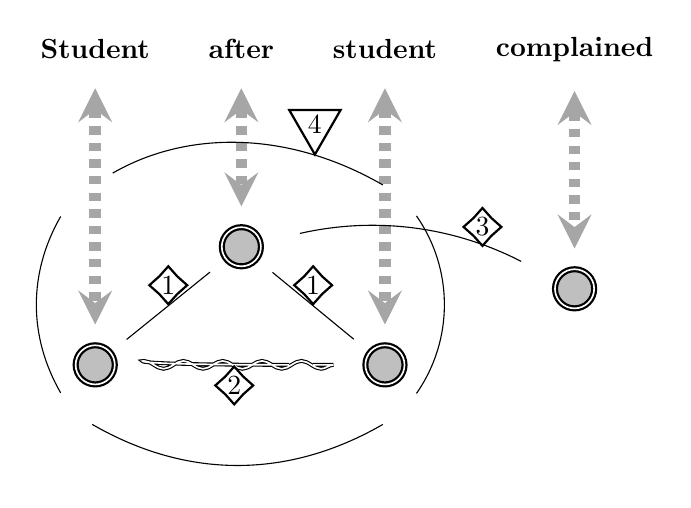
\begin{tikzpicture}

%\tikzset{snake it/.style={decorate, decoration=snake, segment length=5mm, amplitude=15mm}}

%\draw

%\node [s1] at (0,0) {Student};

\node (s1) at (1,1) {\textbf{Student}};
\node (after) [right=5mm of s1] {\textbf{after}};
\node (s2) [right=5mm of after] {\textbf{student}};
\node (complained) [right=5mm of s2] {\textbf{complained}};

\node (s1Rep) [double,draw=black,shape=circle,thick,fill=gray!50,inner sep=.5em,below=3.5cm of s1] {};
\node (afterRep) [double,draw=black,shape=circle,thick,fill=gray!50,inner sep=.5em,below=2cm of after] {};
\node (s2Rep) [double,draw=black,shape=circle,thick,fill=gray!50,inner sep=.5em,below=3.5cm of s2] {};
\node (complainedRep) [double,draw=black,shape=circle,thick,fill=gray!50,inner sep=.5em,below=2.5cm of complained] {};

\draw [ |-,-|, <->, line width = .8mm, draw=gray!70, 
 dashed, double equal sign distance, >= stealth, shorten <= .25cm, shorten >= .25cm ]
 (s1) to (s1Rep);

\draw [ |-,-|, <->, line width = .8mm, draw=gray!70, 
 dashed, double equal sign distance, >= stealth, shorten <= .25cm, shorten >= .25cm ]
(after) to (afterRep);
 
\draw [ |-,-|, <->, line width = .8mm, draw=gray!70,  
 dashed, double equal sign distance, >= stealth, shorten <= .25cm, shorten >= .25cm ]
(s2) to (s2Rep);

\draw [ |-,-|, <->, line width = .8mm, draw=gray!70, 
 dashed, double equal sign distance, >= stealth, shorten <= .25cm, shorten >= .25cm ]
(complained) to (complainedRep);
 
\draw [shorten <= .25cm, shorten >= .25cm ] 
(afterRep) to node [draw=black,shape = star,star points=4,thick,inner sep = 0mm, above] {1} (s1Rep);

\draw [shorten <= .25cm, shorten >= .25cm ] 
(afterRep) to node [draw=black,shape = star,star points=4,thick,inner sep = 0mm,above] {1} (s2Rep);

\node (s1E) [left=-2mm of s1Rep.east]{};
\node (s2E) [left=1mm of s2Rep.west]{};

\draw [shorten <= 2cm, shorten >= .3cm, double, % bend left = 5, 
decorate, decoration={snake, segment length=5mm, amplitude=.5mm}] %, amplitude=15mm]  
(s1E) to node [draw=black,shape = star,star points=4,thick,inner sep = 0mm, below] {2} (s2E);

\draw [shorten <= .5cm, shorten >= .5cm ] 
(afterRep) edge [bend left=20,looseness=1] node [draw=black,shape = star,star points=4,thick,inner sep = 0mm, 
 above, near end ] {3} (complainedRep);

\node (frameTopLeft) [below left = 1.5cm and -.65 cm of s1] {};
\node (frameBottomLeft) [below = 2.5cm of frameTopLeft] {};
\node (frameBottomRight) [right = 3.95cm of frameBottomLeft] {};
\node (frameTopRight) [above = 2.5cm of frameBottomRight] {};

\draw [shorten <= 0.15cm, shorten >= 0.15cm ] 
(frameTopLeft) edge [bend right=30,looseness=1] (frameBottomLeft);

\draw [shorten <= 0.15cm, shorten >= 0.15cm ] 
(frameBottomLeft) edge [bend right=30,looseness=1] (frameBottomRight);

\draw [shorten <= 0.15cm, shorten >= 0.15cm ] 
(frameBottomRight) edge [bend right=35,looseness=1] (frameTopRight);

\draw [shorten <= 0.15cm, shorten >= 0.45cm ] 
(frameTopRight) edge [bend right=30,looseness=1]
node [draw=black,shape = regular polygon,regular polygon sides=3,thick,inner sep = .2mm, 
above, near start, shape border rotate = 180] {4} (frameTopLeft);

%node [draw=black,shape = star,star points=4,thick,inner sep = 0mm, above, 
%bend left=100,looseness=3] {3}

%;


\end{tikzpicture}
\end{minipage}

\hspace{0.1\textwidth}
\begin{minipage}{0.8\textwidth}
			\renewcommand{\labelitemi}{$\blacklozenge$}
	
\begin{itemize}\setlength\itemsep{-.3em}
\item 1 \hspace{12pt}  Head/dependent relation
\item 2 \hspace{12pt}  Argument repetition ({}\BlankAfterBlank{} idiom)
\item 3 \hspace{12pt}  Propositional completion ({}\VisNtoS{})	
			\renewcommand{\labelitemi}{$\blacktriangledown$}
\item 4 \hspace{12pt}  Phrase (modeled as applicative structure), typed as {}\NPl{} 
\end{itemize}
\end{minipage}
\end{figure}
As this shows, the \q{Student after Student} idiom can be notated as, say,
\AfterNSingAndNSingToNPl{} (using \NSing{} and \NPl{} to mean singular
and count-plural nouns, respectively), but with the special case that the \q{argument} to
\i{after} is repeated in both positions, suggesting an unusual degree of repetition,
something frustratingly recurrent: \i{He went on and on}; \i{Car after car passed
us by}; \i{Time after time I got turned down}.
Although I have no problem
treating these constructions as idiomatic plurals, I also contend (on the
premise of phrase-overlap) that the dependent constituents in the \BlankAfterBlank{}
construction can be hooked to other phrases as well (which is why
\q{and [their/his/her] parents} can also be singular, in this case).  I dwell on
this example because it shows how type/functional accounts of phrase structure
can be useful even if we treat phrases more as frames which overlay linguistic
structure, not as rigid compositional isolates.  Each \q{students} variation uses
morphology to nudge cognitive attention in one direction or another, toward events or the
degree to which events are representative of some global property (here of
a student body), or both.  The \NSingToNPl{} transformation is not \i{the}
morphosyntactic meaning, but instead the skeleton on which the full meaning
(via cognitive schema) is designed, its hints solicited.
}
\p{If this analysis has merit, it suggests that a \CAG{}
approach to phrases like \i{many students} or \i{student after student}
(singular-to-plural or plural-to-plural mappings) should be understood not just
as functions among Part of Speech (\POS{}) types but as adding cognitive shading, foregrounding
or backgrounding cognitive elements like events or typicality in some context.
In other words, \i{many students} is type-theoretically \NtoN{} or \NpltoNpl{};
but, in more detail, it adds a kind of cognitive rider attached to the mapping which focuses
cognition in the subsequent discourse onto events (their recurrence and temporal distribution);
similarly \q{student after student} has a \q{rider} suggesting more of a temporal
unfolding.  The second form implies not only that many students complained, but that
the events of these complainings were spread out over some stretch of time.
Each such functional application (mappings between \POS{} understood as linguistic types)
produces not only a resulting \POS{} \q{type}, but also a reconfiguration of cognitive
attitudes toward the relevant situation and context.
Language users have many ways to craft a sentence with similar meanings, and arguably one
task for linguistic analysis is to model the space of choices which are available in a
given situation and represent what specific ideas and effects are invoked by one
choice over others.  It would be an argument in favor of Dependency Grammar if
Dependency-oriented representational models, like Link Grammar, prove to be
especially adept in this modeling.
}
\p{In this analysis, I am already switching to functional and type notions that will be
discussed in greater detail below; my current emphasis is on link grammar as a syntactic
conception, although I have also tried to argue that separating syntax from semantics
can be at most provisional.  Inter-word \q{link pairs} are vehicles for expressing
syntactic rules (like singular/plural agreement) but are also a ground level for
semantic analysis, since we can explain how semantic nuances are carried, in
specific sentences, by the actual link-pairs in evidence (violations to
agreement norms, for example).  These semantic nuances in turn can be given
cognitive interpretations, revealing the syntax-semantics-cognition pattern
which I am sketching here through specific perspectives like Link Grammar and
Type Theory.  Returning to the initial grammatic stage of analysis, however,
my tactics for contrasting overall Dependency and Phrase-Structure paradigms
rest on an implicit picture of how theories should be evaluated.
While such a picture is probably fairly consistent across perspectives, it is still worth
making a little more explicit.
}
\subsection{Explanation and Formality}
\p{Both Dependency and Phrase Structure grammars
presuppose that the fundamental exposition and achievement of their theory involves
formal transformation of linguistic givens, resulting in a more complex data structure
which, to the extent that the theory is correct and useful, models something
of the inner structure of language (\i{qua} abstract formal system and/or cognitive phenomenon).
The \q{data structure} might be a phrase-structure \q{tree} or a graph-like dependency
\q{linkage}, but while these representations have different form they share certain
criteria: they are formally describable systems which allow some structures but reject others;
they are rigorous enough to be given a mathematical (e.g., algebraic) definition;
and they can be expressed in computer code which builds these structures out of
Natural Language artifacts, can verify that an instance of the relevant data structures
satisfies the system rules, and can execute operations which modify the structures.
The phrase trees or word-link graphs are \q{formal substrata} which encapsulate Natural Language
patterns but also are rigidly mathematical and computational.  How thoroughly these substrata
capture linguistic meaning, is therefore directly relevant to questions of whether and
in what degree natural language itself, as social and cognitive, is also formal and computational.
}
\p{Translating NL content into (say) a linked-grammar graph does not make software capable
of \q{understanding} language.  If Dependency Grammar is a reasonable foundation
for linguistics in general, then properly parsing sentences into their
auxiliary graphs is, at most, a step in the direction toward \q{understanding}.
Even this may beg the question of what constitutes a \q{correct} parse: when writing
real-world code, language engineers appear to rely principally on their own intuitions, based
on their familiarity with the underlying theory, the idea they have of what a
\i{correct} \q{re-presentation} looks like (for link grammar, of the correct collection of
link types between the various words).  They then add code to ensure that this representation
is indeed identified by the software in specific examples, and try to do so in such a way
as to generalize to other examples.  This methodology can be gleaned from observing internet chat
sites and other informal research venues; one can witness developers painstakingly constructing
systems which \q{work right} in the sense of producing the interpretation for each sentence
which corresponds with what the human linguists perceive, even for sentences which the
software has never encountered before.  The code is considered reliable the more that
new sentences are \q{correctly} parsed.  Again, \q{correctly} here means, conformant to
linguists' own interpretations; insofar as these are subjective, such conformance is not
conclusive evidence that the transformational algorithms are \q{correct}.
}
\p{In order to assess linguistic \q{competence} (or whatever computational ability may simulate it),
it is needed to check specific \q{behavior} and compare it to some expectation.  The gold standard
for linguistic behavior is just participating in a linguistic community, judged by the community
at large as fully competent and included.  Unfortunately, however \mdash{} at least for those who
want to profit from Artificial Intelligence \mdash{} achieving true \q{language-like behavior} may be
impossible.  Scholarship therefore has to turn toward more limited notions of
competence, such as representational transformation of sentences \mdash{} but since
each theory has its own picture of what sentences should be transformed \i{into},
the justification of competence measures can be circular.  It is the theory which
dictates how the software should act, and the software is deemed \q{intelligent} if it
acts accordingly.  We can be skeptical of such non-theory-neutral conceptions of
\q{intelligence}.  Nonetheless it does count
in theories' favor if they both propose accounts of language structure which
are independently defensible and also can produce computing systems that
reliably and without external direction map language onto those structures.
Language-like behavior then involves producing a transformed representation of
language embodying a particular theoretical conception of
linguistic \q{deep structure}.
}
\p{It would serve Computational-Linguistic theories still further to create systems
that demonstrate behavior which is \q{language-like} on terms less wedded to their
own hypotheses.  More satisfying definitions of linguistic behavior would involve intuitions
of language users in general, not just language experts.  For example, document classifiers
\mdash{} which typically use statistical analysis to predict which topic will be deemed most
relevant for documents like news stories and technical articles \mdash{} again illustate a kind
of transformational representation, converting Natural Language to a formal data structure
(in this case a relatively simple one, naming one or multiple topics from a predefined list).
In this case however a broad user public can provide feedback on how well the system performs.
For another example, artificial translators map language onto formal structures but then
attempt an opposite map, translating the formalized representation into natural-seeming
expressions in a different language.  This case is different in that formal representation is
an intermediary rather than end point of the transformation, but like document classifiers it
is a kind of behavior whose effectiveness can be judged by a large community of speakers.
People who interact with text \q{chat} bots, or talking robots, and feel that the experience
is similar to talking with another person, are also providing evidence of more complete and
larger-scale language-like behavior.  Again, though, it is not now and may never be possible
to engineer intelligent behavior to this level of perfection.  Existing language \AI{} platforms
are flawed but useful, which suggests both that formal re-presentation is an important
step toward language understanding but also that attempts to use these formalisms as a springboard
to more holistic behavior \mdash{} like automated translation, but also extracting practical
information, or gleaning emotion and sentiment \mdash{} are missing something essential.
Doing useful things with or gleaning useful insight from the re-presentational target structures
appears to be a separate problem from that of generating them \mdash{} which calls into question the
degree to which the target structures sufficiently encapsulate linguistic meaning,
even if they reveal structures which are essential to linguistic meaning.
}
\p{This does not have to mean that Natural Language Processing is basically impossible, only
that more modest criteria of \q{correct} \NLP{} systems need to be adopted.  This is complicated
by the fact that artifical language behavior can be flawed but meaningful: \q{Urine shift one
step forward} is an awkward English sentence but its meaning seems clear enough
(this real example comes from a shopping center in New York's Flushing, Queens Chinatown).
We have an intuition that some expressions are \q{incorrect} but not so completely
off-base that they fail to signify anything at all \mdash{} but in this case we need
criteria for how a linguistic performance can be both incorrect \i{and} nonetheless coherent.
}
\p{These issues influence any theory which approaches linguistic competence from the
viewpoint of formal re-presentations, and therefore effectively all branches of
Computational Linguistics.  The reigning assumption appears to be that transformational
representation which converts language to theory-regulated data structures, for which
in many cases the transformation achieved by mechanical algorithms matches that
intuited as most accurate by human experts, serves as \i{prima facie} evidence of
something like computationally-engineered  \q{intelligent (language) behavior}.
This leaves room for language-like behavior to productively replicate dimensions
of language understanding while also being very incomplete: language-like relative
to experts' opinions on deep linguistic structure, not real-world communication.
Structures like link grammar graphs can be essential formal substrata that linguistic expression
relies on to achieve communication, without being the sole medium of this expression.
}
\p{My arguments so far have used Link Grammar as a representative example
of \q{transformational representation} where a computational system
can be judged to reveal some level of language competence, some
kind of \q{language like behavior}, insofar as it translates natural
language expressions to data structures conformant to Dependency
Grammar (and particularly Link Grammar) theory.
As I also just argued, performance \visavis{} structural transformation
may be only tangential to human language, so whatever theory is
built up needs a separate, more philosophical or metatheoretical analysis
to consider how the theory is purported to engage with its phenomena.
But I now take this as a starting point for pivoting the discussion from
grammar to semantics; and will defer until after that speculating
on philosophical implications of the theory thus extended.
}

\subsection{The Chinese Room Revisited}
\p{John Searle's \q{Chinese Room} argument \mdash{} about someone who 
behaves like he understands Chinse by matching characters to responses 
from a vast table \mdash{} is often understood as claiming that 
\q{symbol processing} by itself can never produce real 
understanding, which is \i{semantic} and \i{conceptual}.  
Modern technology makes this thought-experiment less 
hypothtical: automated telephone systems often use a template 
mechanism that is practically like Searle's Chinese Room, 
understanding a limited range of sentencs and producing a limited 
range of responss.  But there are two different kinds of questions we 
can ask in relation to Searle's argument: some 
more philosophical and some more practical.
}
\p{On the philosophical side, we should properly assess the 
important questions as being qualitative and not 
quantitative: it's not as if a synthesized phone system 
is just not a very \i{good} conervsationalist; it's that 
a software machine simply isn't the \i{kind of thing} that 
we can say actually understands language.  This is 
plausible if we say that emotions and empathy are 
intrinsic to language; that we can't properly understand 
language if we do not grasp the emotions residing 
behind expressions.  Indeed, as the case of Grandma's window 
shows, our status as comptent interlopers depends on reading intentions 
behind expressions, and it sems hard to do this if we can't experientially 
empathize with our linguistic partners.
}
\p{Maybe we are now just pushing the important questions back 
to reappear: Ok, can computers be programmed to feel emotions?  
Is there a meaningful distinction between meaningfully, 
experientially having emotions and just behaving as if 
you hav them?  Are emotions themselves somehow 
functionalizable apart from their 
chemical/hormonal substrate so that systems with very 
different physical realization than ours be said 
to have emotions?  I can see how this dbate can go 
different ways.  But I'd also argue that 
any ell-organized dialog about these questions will be 
only tangentially about language \mdash{} in which case, 
neither linguistics nor philosophy 
of language themselves can answer questions about 
what kind of systems (on metaphysical criteria) 
actually \q{do} language.  That would imply 
that affirming a computer's linguistic capabilities 
as \i{real} linguistic understanding is a 
disciplinary non-sequitor for linguistics proper.  
Nothing in the linguist's arsenal either 
dmeonstrates or depends on AI agents actually
\i{being} part of our linguistic community or just 
mimicking language-use to some (sometimes helpful) degree.
}
\p{The more practical questions raised by Searle's 
Chinese Room come into play to the 
degree that the philosophical trail I just sketched 
turns many analyses into a non-starter.  
Consider these two questions to a hypothetical 
automated telephone service:
\begin{sentenceList}\sentenceItem{} What time does the office open?
\sentenceItem{} \label{itm:phone} What time does train 100 depart from Newark?
\end{sentenceList}
While we can see a template holding canned responses for both 
cases, (\ref{itm:phone}) needs to do more than just 
fit the input to the nearest pattern; it has 
to pull out the dynamically variant details 
(train \i{100} from \i{Newark}) and use those to 
fill in details in the response.  This is something 
like \i{parsing} the original question.  So we can add 
bits and pieces of genuine linguistic processing 
to a minimal response-template system \mdash{} a real version of 
what Searle appeared to imagine in the Room.  With enough 
added features the primitive template-driven 
kernel can evolve into a complex AI-powered 
Natural Language Processor.  
}
\p{In that case we may imagine that \q{language 
understanding} exists on a spectrum.  The primitive 
telephone service and an erudite bard may lie on 
opposite ends of a spectrum, but they share a spectrum 
between them.  In this case, their differences are 
quantitative more than qualitative.  The bard just 
has more \i{features} we associate with total 
linguistic behavior.
}
\p{However, this quantitative view still leaves open the question 
of where among the \q{features} do we have something 
that actually drives language competence?  Searle's 
Chinese Room helps point out these questions: 
it's reasonable to say that the simplest template-response 
system does not really understand language at all, since it 
is a pattern-matching system that does not 
have any structural relation to language itself.  
Analogous capabilities can be developed for a system 
which matches any kind of input to a pattern directing 
an output, based on any metric of similarity.  
The patterning reflects an actual \i{linguistic} 
parse only insofar as it selects elements 
via syntactic criteria, like grasping the 
non-template variables as \i{100} and \i{Newark}.  
So, even if the holistic behavior different systems 
lies on a linguistic-competence sclae, not 
all \i{parts} of the system seem to bear the weight 
of actually \i{realizing} linguistic competence equally.
}
\p{One reading of the Chinese Room is that \i{no} 
part of a system is truly 
linguistic.  This includes the argument that 
holistically the Chinese Room \i{does} 
speak Chinese: Searle's discussion 
suggests that no \i{part} understands Chinese, but 
if we can imagine the entire room as a single 
system this \q{entity} can be treated as a fluent 
Chinese speaker.  Even if we reject that analysis, 
we could agree that, even among humans, \i{parts} of 
our language system arguably do not understand language: 
not nerve cells, not neural clustes for auditory 
processing, or sytax, or conceptualization, etc.  
It is us, the whole system, that 
uses language.  The reason why \q{holistic} claims 
that \q{the entire room} speaks Chinese sound dubious 
may not be because something is 
\i{structurally} lacking in that whole
system, but because it's not the kind of whole 
system \mdash{} with one body, one consciousness, one 
personhood \mdash{} that we think of as a conversant. 
}
\p{Those who find Searle's analysis compelling probably believe 
that there \i{is} some meaningful difference between us 
(or at least people fluent in Chinese) and 
the Chinese Room.  A further alternative, however, 
is that \i{we} are not language-usrs, at least not 
in the way we think we are.  This 
claim can be expounded as follows: the philosophy 
of language, interactively with linguistics, seems 
to be looking for some essntial kernel of linguistic 
capability that distinguishes us from AI engines or 
template-response system.  That is, AI-skeptics want to 
sift through all the models of processes within 
languages, the central domains in linguistics, 
and find the few genreas of linguistic processing that are 
unique to human language \mdash{} and computationally 
intractable.  These would be the smoking gun evidnce that no 
artifical system can equate to human language-use because 
there is some essential stage in the linguistic 
pipeline that computers computationally 
can't realize.
}
\p{However, even if we accept premises that the Chinese Room case 
suggests this analysis and moreover it agrees with our 
underlying intuitions, there remains 
the possibility that computers are indeed lacking 
some stage associated with language \mdash{} but it 
is not a \i{linguistic} stage.  If something like 
an Interface Theory of Meaning is correct, all linguistic 
processing is intermediary to some other 
cognitive layer: and perhaps the human quintessence 
lies on the far side, so it both limits what computers can 
linguistically achieve and lies outside of linguistics 
proper.
}
\p{}
\p{}
\p{}

\section{Cognitive Grammar and Type Theoretic Semantics}
\p{The emergence of Dependency Grammar as a \i{computational} approach has some broad
implications.  The historical preference for phrase-structure foundations  \mdash{} among
those who actually build Natural Language Processing code libraries, in disciplines
related to Artifical Intelligence \mdash{} arguably reflects how phrase structure more
cleanly models a theory of linguistic meaning and signification based on
\q{symbolic logic} \mdash{} a theory that the \i{meaning} of a complete and self-contained
linguistic expression is the logical state of affairs which it asserts or in other
ways connotes.  Correlated with this assumption is the idea that phrase structure
logically transforms its constituent parts; so from the word \q{students} we
can form the phrase \q{many students} to designate a kind of plurality \mdash{} a plural
set but also, more specifically, a set which is reasonably large relative to some context.
In the hierarchical model presented by these norms, phrases subsume the roles of
individual words and represent discrete semantic units with respect to still larger phrases.
}
\p{It is certainly true that one role for phrases is to satisfy a semantic niche \mdash{} often
a place occupied in other (or even the same) language with single words, or vice-versa.
The French \q{laisse tomber} translates the English \q{drop}, for example; and
\q{parliamentarian} is a more exotic version of \q{Member of Parliament}.  There is no
evident pattern for when a single concept is conveyed, in one language or another,
by a single word or a multi-word phrase.  Moreover, the meanings of phrases are influenced
by semantic conventions no less than are individual words, and they are not solely a product
of phrase constituents.  Semantics is guided by what people need to talk and write about often; when
events in a linguistic community call for some fairly rigid and repeatable designation for
an important concept, the resources of language adjust to provide that role, either through a
complete neologism, or a lexical variant \mdash{} a new usage; or the entrenchment of a phrase.
In current events, the expression \q{Syrian Refugees} recurs when discussing people
displaced by the Syrian civil war, and potentially other interrelated conflicts also;
convention seems to allow that nominal \q{Syrian} Refugees don't have to be Syrian nationals.
The meaning of the phrase is fixed by its niche in familiar discourse more than
by its literal form.  Phrases
exhibit conventionalization and usage pressures analogous to single words; which lends
credance to the notion that phrases subsume the role of single words, and that the semantic
contribution of words to sentences is determined through the phrases where they occur.
}
\p{On the other hand, it is well established that words' contributions are not \i{wholly}
subsumed by their surrounding phrase-structure.  The famous joke about the Holy Roman
Empire \mdash{} or its reprise in the current line that the Islamic State is neither Islamic
nor a State \mdash{} point to evidence that as language-users we still hear the individual
words outside their phrase context.  To subsume a word into a phrase is also to suggest a
particular semantic (and pragmatic, real world) interpretation, one which conversants
may challenge.\footnote{How literally to take phrases is a notorious source of political controversy:
recall debates about the relevance of Afghanistan for Iraq, in US policy, and
Rudy Giuliani saying \q{There \i{is} Al Qaeda in Iraq \mdash{} it's called, \sq{Al Qaeda in Iraq}}.
}
}
\p{Arguably, joking or titular cases like \q{Holy Roman Empire} can be
relegated to thematic margins, especially if we accept formal-logical construals of
what semantics is all about, with an \i{a priori} contrast between Semantics and
Pragmatics, the former rooted in \i{states of affairs} and only the latter addressing
rhetoric and usage.
Counter to this counter-argument, however, we can observe that different phrases imply
different degrees of \q{autonomy} to their constituents, and different degrees of
coherence or unification into a single idea.  Some phrases act as direct substitutes
for single concepts (like \q{Member of Parliament}) where it seems mostly historical
accident that a phrase rather than a word emerged as the most popular; but many other
phrases have more complex usage scanarios, including everyday expressions that don't have
special rhetorical or sociolinguistic conventions that would make them tangential to
semantic or syntactic analysis proper.  Moreover, many of these examples are similar to
those used by Cognitive Grammar to challenge the syntax/semantic distinction and argue for
\q{morphosyntactic} models as reciprocating cognitive formations, not abstract language-rules.
}
\p{For example, in Ronald Langacker's \i{Foundations of Cognitive Grammar}, the sentence
\begin{sentenceList}\sentenceItem{} Three times, students asked an interesting question
\end{sentenceList}
is used to demonstrate how
grammatical principles follow from cognitive \q{construals} of the relevant situations,
those which language seeks to describe or takes as presupposed context.\footnote{For example, \cite[pp. 119 and 128]{LangackerFoundations},
discussed by \cite[p. 189]{LineBrandt}, and \cite[p. 9]{EstherPascual}.
}
In particular, Langacker argues that \q{students} and \q{question} can both be either singular or
plural: syntax is open-ended here, with neither form more evidently correct.  Langacker uses this
example to make the Cognitive-Linguistic point that
we assess syntactic propriety relative to cognitive frames and conversational context.  In this
specific case, we are actually working with two different cognitive frames which are interlinked
\mdash{} on the one hand, we recognize distinct events consisting of a student asking a question, but
the speaker calls attention, too, to their recurrence, so the events can also be understood
as part of a single, larger pattern.  There are therefore two different cognitive foci, at two
different scales of time and attention, a \q{split focus} which makes both singular and plural
invocations of \q{student} and \q{question} acceptable.
}
\p{Supplementing this analysis, however, we can additionally focus attention directly on
grammatical relations.  The words \q{student} and \q{question} are clearly linked as the subject and
object of the verb \q{asked}; yet, contrary to any simple presentation of rules,
no agreement of singular or plural is required between them (they can be singular and/or plural in
any combination),  Moreover, this anomaly is only in force due to the context established
by an initial phrase like \q{Three times}; absent some such framing, the singular/plural
relation would be more rigid.  For example, \q{A student asked interesting questions} would
(in isolation) strongly imply \i{one} student asking \i{several} questions.  So the initial
\q{Three times} phrase alters how the subsequent phrase-structure is understood while remaining
structurally isolated from the rest of the sentence.  Semantically, it suggests a
\q{space builder} in the manner of Gilles Fauconnier or Per Aage Brandt
\cite{Fauconnier}; \cite{PerAageBrandt}, but we
need to append Mental Space analysis with theory of how these spaces
influence syntactic acceptability, which would seem to be logically prior to the stage where Mental Spaces
would come in play.  This complex interplay of phrase-structures
is hard to accommodate from the grammar-hierarchy perspective.  There seems to be
no way to break down this example sentence into a tree-like phrase hierarchy wherein each
phrase, considering the semantic concept which it is apparently tasked to put into words,
can be seen to function in isolation.  The mapping of the sentence to a logical
substratum would be more transparent with a sentence like \q{Three students asked
interesting questions}; that sentence is a more direct translation of the facts
which the original sentence conveys.  But this \q{more logical} sentence has different
connotations than the sentence Langacker cites; the original sentence places the emphasis
elsewhere, calling attention more to the idea of something temporally drawn-out,
of a recurrence of events and a sense of time-scale.  The \q{more logical} sentence
lacks this direct invocation of time scale and temporal progression.
}
\p{We can say that the \q{Three students} version is a more direct statement of fact, whereas
Langacker's version is more speaker-relative, in the sense that it elaborates more
on the speaker's own acknowledgment of belief.  The speaker retraces the steps of her
coming to appreciate the fact \mdash{} of coming to realize that the \q{interesting questions}
were a recurrent phenomenon and therefore worthy of mention.  By situating expression
relative to cognitive process rather than to the facts themselves, the sentence
takes on a structure which models the cognition rather than the states of affairs.
But this shift of semantic grounding from the factual to the cognitive also apparently
breaks down the logical orderliness of the phrase structure.  \q{Three times}, compared
to \q{three students}, leads to a morphosyntactic choice-space which is
\q{underdetermined} and leaves room for speakers' shades of emphasis.
}
\p{This is not an isolated example.  Many sentences can be provided with similar
phrase-structure complications, particularly with respect to singular/plural agreement.
\begin{sentenceList}\sentenceItem{} Time after time, tourists (a tourist) walk(s) by this building
with no idea of its history.
\sentenceItem{} The streets around here are confusing; often people (someone)
will ask me for directions.
\sentenceItem{} Student after student came with their (his/her)
paper to compain about my grade(s).
\sentenceItem{} Student after student \mdash{} and their (his/her) parents
\mdash{} complained about the tuition increase.
\end{sentenceList}
On a straightforward phrase-structure reading, \q{Student after student} reduces to an
elegant equivalent of \q{Many students}, with the rhetorical flourish abstracted away
to a logical form.  But our willingness to accept both singular and plural agreements
(his/her/their parents, grades, papers) shows that clearly we don't simply substitute
\q{Many students}; we recognize the plural as a logical gloss on the situation but
engage the sentence in a more cogntively complex way, recognizing connotions of temporal
unfolding and juxtapositions of cognitive frames.  The singular/plural underdeterminism
is actually a signification in its own right, a signal to the listener that the
sentence in question demands a layered cognitive attitude.  Here again, syntactic
structure (morphosyntactic, in that syntactic allowances are linked with
variations in the morphology of individual words, such as singular or plural form)
serves to corroborate conversants' cognitive frames rather than to model logical
form.
}
\p{This is not to say that phrase-structure paradigms are refuted by these examples.  Cases
like these can be accommodated by layering new structural rules, such as
allowing exceptions for singular/plural agreement in the presence of certain
\q{lead-in} phrases like \q{Three times}.  It is not even accepted that these
examples clearly favor inter-word relations (as language formalization, in preference over
phrase-structure trees) \mdash{} cases like \q{Student after student} have
also been used \i{against} Dependency Grammar on the argument
that there is not a clear \q{single} word, in that phrase,
which should be seen as linking with words elsewhere in the sentence
\cite[pp. 400-401]{MullerBook}, \cite[p. 2]{MullerPDF}.  It
seems arbitrary to select either \q{student}, or \q{after}, as \q{the}
representative of the phrase to link with \mdash{} for example \mdash{} the verb
\q{complained}; on that argument, the least arbitrary analysis is to
treat the phrase as a whole as a single unit for purposes of grammatic
linkage.  In short, both paradigms have potential problems with these example.
Considering \q{Student after student} as an encapsulated phrase leaves
the singular/plural flexibility in the continuation of the sentence unexplained
(\q{Many students compained about \qmarkdubious{}his grade} is clearly dubious, so
\q{Many students} is not a direct substitution). But bracketing the phrase
when decribing the sentences' \q{linkage} leads
to an apparently arbitrary choice when it comes time to notate the subject/verb
linkage for \q{complained}.  I will address this particular ambiguity later;
but for now I'll just point out that a simplistic reading of
both Dependency and Phrase-Structure ideas seems to run aground.
}
\subsection{Comparing paradigms}
\p{Since Computational-Linguistic paradigms find practical expression in code
libraries, there are some options to assess competing theories empirically
\mdash{} comparing libraries' speed, accuracy, ease of use, and how readily can they be
modified in light of new research.  Arguably, however, the
quality of a code library does not automatically reflect the accuracy of
its underlying linguistic paradigms (as opposed to the skill, foresight, and
resources of its programmers); not to mention that more complex analyses of
human language may be both more correct and also harder to express in code.
There is, in any case, no apparent consensus amongst linguists and programmers that one
or another language theory has proven computationally preferable.  Another approach to
theory-comparison involves considering the range of linguistic phenomena which different methods can explain, without resorting to ad-hoc compilations of exceptions and
special cases.  Arguably, here, Dependency Grammar provides more
straghtforward explanations.  For example, the internal structure of phrases seems to
lend specificity and nuance to their meaning in ways that get lost when
trying to replace phrases with logico-semantic equivalents.
\q{Student after student} is not losslessly substitutable with \q{Many students},
and the former phrase has a temporal and multi-tier cognitive implication which
the latter discards.  The second phrase is compatible with \q{Many students}
complaining \i{at one time}, as well as drawn out over time; the former phrase
appears to clarify that the second kind of situation is the intended meaning,
Of course, in context, the two phrases may be understood to have similar meanings;
but this is a product of how the linguistic structure relates to its presumptive
conversational context, not to an intrinsic semantic equivalence.  I will
now consider these and other examples to discuss the dependency/phrase-structure
contrast in a little more detail.
}
\p{The contrast between the phrases \q{Student after student} and \q{Many students}
cannot be based on \q{abstract} semantics alone \mdash{} how the evident temporal implications of the
first form, for example, are concretely understood, depends on conversants' mutual recognition
of a relevant time frame.  The dialog may concern a single day, a school year, many
years.  We assume that the speakers share a similar choice of time \q{scale}
(or can converge on one through subsequent conversation).  \i{Some} time-frame
is therefore presupposed in the discursive context, and the first phrase invokes
this presumed but unstated framing.  The semantics of the phrase are therefore somewhat open-ended:
the phrase \q{hooks into} shared understanding of a temporal cognitive framing without referring
to it directly.  By contrast, the second phrase is less open-ended: it is consistent with both
a more and less temporally protracted understanding of \q{many}, but leaves such details (whatever
they may be) unsignified.  The factual circumstance is designated with a level of abstraction that sets
temporal considerations outside the focus of concern.  The second phrase is therefore both
less open-ended and also less expressive: it carries less detail but accordingly also relies
less on speaker's contextual understanding to fill in detail.
}
\p{Clearly the two phrases are therefore semantically different; but notice also that the
semantic properties of the first phrase are due explicitly to its internal structure.
The temporality implicatures could be expressed in a more \q{purely} semantic
fasion with a choice of wording, like \q{a procession of students complained}.  This
would rely on the conventional meaning of \q{procession} (or \q{stream}, \q{sequence},
etc.) to provide the expressive \q{time} dimension.  But the \q{Student after student}
phraseology achieves this effect more economically and with more \q{oomph} because the
internal repetition in the phrase itself effectively models the recurrence it
seeks to feature semantically.  Here linguistic form actually does reproduce
factual structure, like a syntactic version of onomatopoeia.  This fact of internal structure
clearly can only be fully modeled by taking seriously the exact composition of the phrase, not
treating the phrase-structure as a convention fully subsumed by a semantic role.
}
\p{In addition, aside from the expressive detail which depends on the actual phrase
structure (which therefore cannot be summarized away), this inner structure also
governs morphosyntactic possibilities over all.  \q{A procession of students}
captures a similar temporal progression but also fully absorbs \q{student} in a plural
guise, and \q{A procession of students complained about \qmarkdubious{}his grade} is straightforwardly
ungrammatical.  In Langacker's \q{Three times} example, the inter-word
\q{linkage} captures the aforementioned complexities in a reasonably non-arbitrary
way, I believe.  \q{Student} is linked as subject-to-verb with \q{asked}, and as
subject-to-object with \q{question}.  It is true that these link-pairs seem to
violate agreement norms, but there is nothing in the Link Grammar paradigm \mdash{} which
practices Dependency Grammar with a rather detailed and intricate
inventory of inter-word relations, or \q{links} \mdash{} mandating that
\i{all} link-pairs exhibit forced agreement (like singular/plural).  Agreement, when it
applies, is a property \i{of} link pairs.  There is also an implicit
(cross-phrasal) link between \q{student} and \q{Three} \mdash{} clarifying that, considered
in its entirely, the sentence is about three students precisely \mdash{} and the presence of
this kind of link alters how the other links connecting to the word \q{student} are
assessed.  In particular, this latter link stipulates that the word \q{student} is being
simultaneously understood in both a plural and a singular sense, so it permits
singular \i{and} plural link forms which, more commonly, could only be
singular \i{or} plural.  So link grammar can offer an elegant analysis of
singular/plural \q{underdeterminism}, expressed in the
same underlying graph-context terminology as most other link-grammar theorizing.
It would be unfair to use this as a case against Phrase Structure grammars without a
detailed presentation of how these grammars would handle such a case in turn, but
I'd argue that link grammar accommodates this complex example with relatively little
departure from its underlying theoretical and notational or presentational commitments.
}
\p{While my previous examples contrasted Phrase Structure and Dependency
Grammars in terms of their resources for explaining sentences with
unusual semantic patterns but relatively clear meanings (in context),
another form of comparison can address actual ambiguity.  Consider
\begin{sentenceList}\sentenceItem{} The Maple Leafs failed to win in overtime for the
first time this year.
\sentenceItem{} The Maple Leafs failed for the first time this year
to win in overtime.
\end{sentenceList}
The first can mean either that the Leafs had won \i{all} or \i{none}
of their prior overtime games.  From a phrase-structure perspective,
we have to image that \q{to win in overtime} can \q{migrate} so we
hear it as in the second version of the sentence.  For more inter-word
grammars, the alternation is simpler: \q{for}, initiating the phrase
\q{for the first time}, can be linked with either \i{failed} or
\i{win} \mdash{} notationally, it amounts to the presence or absence of one
graph-edge, when the syntax is represented as a graph with
inter-word labels for link kinds.  This could be a distinction without
a real difference, since choosing which inter-word link to recognize
triggers linking in the rest of the phrase along with it.
But perhaps reflecting on how we process the ambiguity \mdash{} realizing
that there are two competing parses and deciding which is the one
intended \mdash{} we picture the alternatives more as \q{horizontal}
options for connecting threads across the sentence,
more so than a \q{vertical} organization where
we hear \q{for the first time} as \q{contained} in a larger phrase.
My own feeling is of exploring competing relational patterns more than
exploring different ways that the phrases can be nested inside each
other.
}
\p{That being said, how much of our sense of ambiguity (or clarity, for
that matter) is driven by meaning, not form?  The \q{double parse}
just examined does not always generalize to similar cases:
\begin{sentenceList}\sentenceItem{} The Maple Leafs failed to win two consecutive games
for the first time this year.
\end{sentenceList}
The reading as in \q{this is the first time they failed to win two
consecutive games} makes no sense \mdash{} unless you've won every game,
but perhaps the first, you've at some point lost after a win.  Is this
case anomalous, where a syntactic ambiguity idiosyncratically fails to
yield logically plausible readings?
The ambiguity is found in \i{failed to make the playoffs
for the first time since 2013}, and many \i{for the first time this
season} cases, like \i{beat the Habs}, \i{sell out the arena},
\i{score a goal in the first period}.  But \q{failed to score a goal}
is almost surely read that they \i{did} score in every prior game.
Do we hear the construction as intrinsically ambiguous, and reject one
reading only when it is clearly flawed pragmatically?
}
\p{If we believe that language understanding unfolds in a predictable
operational sequence, then we should assume that both parses are
deemed plausible, and semantic considerations only retroactively
eschew one reading (if they do so at all).  This would explain why in
many cases the ambiguity persists enough to cast the practically
intended meaning in doubt.  But that account does not consider the
temporality of language itself; the hearer does not know in advance
that a trailing phrase like \q{for the first time this season} is coming,
and starts to make sense of the sentence up to there; once then hearing or
reading the addendum, the audience instinctively has to interpret the
final phrase as deliberately inserted to modify an already-complete
idea.  On this analysis, the addendum is initially approached as a
performative detail, something said for a reason to be determined \mdash{}
it is not structurally necessary to make the sentence well-formed.
Perhaps we then try to fit the last phrase into the sentence both
syntactically and semantically, together, triggered by a pragmatic
phenomenon (the speaker's choice to add on to a seemingly complete
thought) which then becomes logically prior to both syntax and
semantics.  If this is plausible, it supports an inter-word relational
model because we are forming a picture of language structure
relationally, assimilating new words and phrases to those already
heard by linkings referring back in time, rather than waiting until we
are sure we have a complete sentence and then treating it as a static
structure to vertically reconstruct.
}
\p{The examples I have used so far may also imply that a choice of phrase structure is
always driven by semantic connotations of one structure or another;
but seemingly the reverse can happen as
well \mdash{} speakers choose a semantic variant because its grammatic realization lends a useful
organization to the larger expression.  There are many ways to say \q{many},
for example: \i{a lot of},
\i{quite a few}, not to mention \q{time after time} style constructions.  Whatever their
subtle semantic variations, these phrases also have different syntactic properties:
\i{Quite a few} is legitimate as standalone (like an answer to a question);
\i{A lot of} is not, and \i{A lot} on its own is awkward.  On the other hand the \q{of} in
\i{A lot of} can \q{float} to be replicated further on: \q{A lot of students, of citizens,
believe education must be our top priority} sounds more decorous than the equivalent sentence with the
second \q{of} replaced by \q{and}.  If the cadence of that sentence appeals to the speaker, then
such stylistic preference will influence taking \q{A lot of} as the \q{many} variant of choice.
So speakers have leeway in choosing grammatic forms that highlight one or another aspect of
situations; but they also have leeway in choosing rhetorical and stylistic pitch.  Both cognitive
framings and stylistic performance can be factored when reconstructing what compels the
choice of one sentence over alternatives.
}
\p{One consequence of these analyses, should they be accepted, is that grammar
needs to be approached holistically: the grammatic structure of phrases cannot,
except when deliberate oversimplification is warranted, be isolated from
surrounded sentences and still larger discourse units.  Semantic roles
of phrases have some effect on their syntax, but phrases are nonetheless chosen
from sets of options, whose variations reflect subtle semantic and syntactic
maneuvers manifest at super-phrasal scales.  The constituent words of phrases retain some
autonomy, and can enter into inter-word and phrasal structures with other words outside their
immediate phrase-context.  We can still apply formal models to phrase
structure \mdash{} for example, Cognitive and Applicative Grammar (\CAG{}) considers phrases
as \q{applications} of (something like) linguistic or cognitive \q{functions},
in the sense that (say) an adjective is like a \i{function} applied to a noun,
to yield a different noun (viz., something playing a noun's conceptual role)
\cite{Descles2010}.
I will consider related \q{functional} and (by extension) Type-Theoretic
approaches in the next section.  But we should not read these transformations
\mdash{} like \i{Syrian refugee} from \i{refugee} \mdash{}
too hastily as a purely semantic correlation within a space of denotable concepts
\mdash{} \i{such that} the new concept wholly replaces the
contained parts, which then cease to have further linguistic role and effect.
Instead, applicative structures represent shifts or evolutions in
mental construal, which proceed in stages as conversants form
cognitive models of each others' discourse.  Even if phrase structure
sets landmarks in this unfolding, phrases do not wholly subsume their
constituents; the parts within phrases do not \q{vanish} on the higher scale,
but remain latent and may be \q{hooked} by other, overlapping phrases.
This argument rests on a vantage point from semantics as well as syntax;
therefore, I will discuss it briefly at present (I return to
this analysis at greater length in the next section).
}
\p{Consider the effect of \q{Many students complained}.  Propositionally, this appears
to say essentially that \i{students} complained; but, on hermeneutic charity, the
speaker had \i{some} reason to say \q{many}.  The familiar analysis is that
\q{many} suggests relative size; but this
is only half the story.  If the speaker chose merely \i{students complained}, we would hear an assertion
that more than one student did, but we would also understand that there were several
occasions when complaints happened.  Adding \q{many} does not just
imply \q{more} students, but suggests a mental shift away from the particular episodes.
In the other direction, saying \i{a student complained} is not just
asserting how at least one student did so, but
apparently reports one specific occasion (which perhaps the speaker wishes to
elaborate on).  In other words, we cannot really capture the singular/plural semantics,
or different varieties of plural, just by looking at the relative size of implied
sets; we need to track how representations of singleness or multitude imply
temporal and event-situational details.  So \i{a student complained} focuses not
on the numeric count of one, but on a singular event (unlike
\q{\i{only one} student complained}); \i{students complained} focuses not on the
plural measure of students involved, but on the fact that a certain type
of event happened several times.  \i{Many students complained}
focuses not on sheer number (unlike \i{a large number of students complained}),
but rather on the implication that complaints were widespread enough to represent
a significant sample, perhaps a majority sentiment, among the student body.
The semantics of the former two forms seems to focus attention
on the \i{events} of complaining, while the \i{many students} construction seems
to focus more on their suggesting a prevailing attitude.  \q{Students complained}
seems to single out each event as distinct, even though there are several of
them; whereas \i{Many students complained} seems to construe the
events as each resembling the other, to the point where they partly
lose their individuality.  \q{Isolated events},
in the English idiom, are those which are atypical; as we cognitively
shift from the events as discrete to recurring patterns, they become
suggestive of a larger state of affairs.  By implication, if many students
complained, many other students may be unhappy; the extent of students'
unrest is no longer measurable by the multiplicity of the complaining-events.
}
\p{Against this backdrop, \i{Student after student complained} captures both dimensions,
implying both a widespread unrest among the student body and also
temporal recurrence of complainings.
Formal models of syntax and semantics often borrow notation from formal
language theory; for example, notations for Parts of Speech lifted
from functional programming languages.\footnote{A note on notation: I adopt the Haskell convention (referring to the Haskell
programming language and other functional languages) of using arrows both between
parameters and before output notation, but for visual cue I add one dot above the
arrow in the former case, and two dots in the latter: \argsToReturn{}.
I use \N{} for the broadest designation of nouns (the broadest
noun type, assuming we are using type-theoretic principles),
with extra markings for more specific types (in principle
similar notation could be adopted for verbs, propositions, and so on).
}
This notation can help us picture the \q{flow} of ideas building up
to a complete sentence, formally represented via type theory
(where sentences reveal a type hierarchy culminating in a self-contained idea,
that is, a proposition); more informally we can picture a similar
\q{conceptual} flow tracing how listeners come to make sense of the
language they encounter enunciated by speakers.  By way
of illustration, Figure ~\ref{fig:ESA} shows a
Depency-style descructuring, with implicit type annotations.  \begin{figure}
\caption{Dependency-style graph with argument repetition}	
\label{fig:ESA}
\vspace{1em}
\hspace{0.15\textwidth}	
\begin{minipage}{0.7\textwidth}
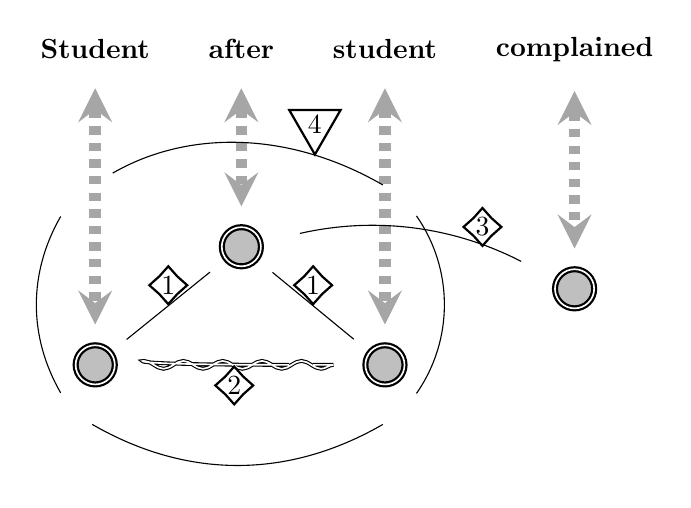
\begin{tikzpicture}

%\tikzset{snake it/.style={decorate, decoration=snake, segment length=5mm, amplitude=15mm}}

%\draw

%\node [s1] at (0,0) {Student};

\node (s1) at (1,1) {\textbf{Student}};
\node (after) [right=5mm of s1] {\textbf{after}};
\node (s2) [right=5mm of after] {\textbf{student}};
\node (complained) [right=5mm of s2] {\textbf{complained}};

\node (s1Rep) [double,draw=black,shape=circle,thick,fill=gray!50,inner sep=.5em,below=3.5cm of s1] {};
\node (afterRep) [double,draw=black,shape=circle,thick,fill=gray!50,inner sep=.5em,below=2cm of after] {};
\node (s2Rep) [double,draw=black,shape=circle,thick,fill=gray!50,inner sep=.5em,below=3.5cm of s2] {};
\node (complainedRep) [double,draw=black,shape=circle,thick,fill=gray!50,inner sep=.5em,below=2.5cm of complained] {};

\draw [ |-,-|, <->, line width = .8mm, draw=gray!70, 
 dashed, double equal sign distance, >= stealth, shorten <= .25cm, shorten >= .25cm ]
 (s1) to (s1Rep);

\draw [ |-,-|, <->, line width = .8mm, draw=gray!70, 
 dashed, double equal sign distance, >= stealth, shorten <= .25cm, shorten >= .25cm ]
(after) to (afterRep);
 
\draw [ |-,-|, <->, line width = .8mm, draw=gray!70,  
 dashed, double equal sign distance, >= stealth, shorten <= .25cm, shorten >= .25cm ]
(s2) to (s2Rep);

\draw [ |-,-|, <->, line width = .8mm, draw=gray!70, 
 dashed, double equal sign distance, >= stealth, shorten <= .25cm, shorten >= .25cm ]
(complained) to (complainedRep);
 
\draw [shorten <= .25cm, shorten >= .25cm ] 
(afterRep) to node [draw=black,shape = star,star points=4,thick,inner sep = 0mm, above] {1} (s1Rep);

\draw [shorten <= .25cm, shorten >= .25cm ] 
(afterRep) to node [draw=black,shape = star,star points=4,thick,inner sep = 0mm,above] {1} (s2Rep);

\node (s1E) [left=-2mm of s1Rep.east]{};
\node (s2E) [left=1mm of s2Rep.west]{};

\draw [shorten <= 2cm, shorten >= .3cm, double, % bend left = 5, 
decorate, decoration={snake, segment length=5mm, amplitude=.5mm}] %, amplitude=15mm]  
(s1E) to node [draw=black,shape = star,star points=4,thick,inner sep = 0mm, below] {2} (s2E);

\draw [shorten <= .5cm, shorten >= .5cm ] 
(afterRep) edge [bend left=20,looseness=1] node [draw=black,shape = star,star points=4,thick,inner sep = 0mm, 
 above, near end ] {3} (complainedRep);

\node (frameTopLeft) [below left = 1.5cm and -.65 cm of s1] {};
\node (frameBottomLeft) [below = 2.5cm of frameTopLeft] {};
\node (frameBottomRight) [right = 3.95cm of frameBottomLeft] {};
\node (frameTopRight) [above = 2.5cm of frameBottomRight] {};

\draw [shorten <= 0.15cm, shorten >= 0.15cm ] 
(frameTopLeft) edge [bend right=30,looseness=1] (frameBottomLeft);

\draw [shorten <= 0.15cm, shorten >= 0.15cm ] 
(frameBottomLeft) edge [bend right=30,looseness=1] (frameBottomRight);

\draw [shorten <= 0.15cm, shorten >= 0.15cm ] 
(frameBottomRight) edge [bend right=35,looseness=1] (frameTopRight);

\draw [shorten <= 0.15cm, shorten >= 0.45cm ] 
(frameTopRight) edge [bend right=30,looseness=1]
node [draw=black,shape = regular polygon,regular polygon sides=3,thick,inner sep = .2mm, 
above, near start, shape border rotate = 180] {4} (frameTopLeft);

%node [draw=black,shape = star,star points=4,thick,inner sep = 0mm, above, 
%bend left=100,looseness=3] {3}

%;


\end{tikzpicture}
\end{minipage}

\hspace{0.1\textwidth}
\begin{minipage}{0.8\textwidth}
			\renewcommand{\labelitemi}{$\blacklozenge$}
	
\begin{itemize}\setlength\itemsep{-.3em}
\item 1 \hspace{12pt}  Head/dependent relation
\item 2 \hspace{12pt}  Argument repetition ({}\BlankAfterBlank{} idiom)
\item 3 \hspace{12pt}  Propositional completion ({}\VisNtoS{})	
			\renewcommand{\labelitemi}{$\blacktriangledown$}
\item 4 \hspace{12pt}  Phrase (modeled as applicative structure), typed as {}\NPl{} 
\end{itemize}
\end{minipage}
\end{figure}
As this shows, the \q{Student after Student} idiom can be notated as, say,
\AfterNSingAndNSingToNPl{} (using \NSing{} and \NPl{} to mean singular
and count-plural nouns, respectively), but with the special case that the \q{argument} to
\i{after} is repeated in both positions, suggesting an unusual degree of repetition,
something frustratingly recurrent: \i{He went on and on}; \i{Car after car passed
us by}; \i{Time after time I got turned down}.
Although I have no problem
treating these constructions as idiomatic plurals, I also contend (on the
premise of phrase-overlap) that the dependent constituents in the \BlankAfterBlank{}
construction can be hooked to other phrases as well (which is why
\q{and [their/his/her] parents} can also be singular, in this case).  I dwell on
this example because it shows how type/functional accounts of phrase structure
can be useful even if we treat phrases more as frames which overlay linguistic
structure, not as rigid compositional isolates.  Each \q{students} variation uses
morphology to nudge cognitive attention in one direction or another, toward events or the
degree to which events are representative of some global property (here of
a student body), or both.  The \NSingToNPl{} transformation is not \i{the}
morphosyntactic meaning, but instead the skeleton on which the full meaning
(via cognitive schema) is designed, its hints solicited.
}
\p{If this analysis has merit, it suggests that a \CAG{}
approach to phrases like \i{many students} or \i{student after student}
(singular-to-plural or plural-to-plural mappings) should be understood not just
as functions among Part of Speech (\POS{}) types but as adding cognitive shading, foregrounding
or backgrounding cognitive elements like events or typicality in some context.
In other words, \i{many students} is type-theoretically \NtoN{} or \NpltoNpl{};
but, in more detail, it adds a kind of cognitive rider attached to the mapping which focuses
cognition in the subsequent discourse onto events (their recurrence and temporal distribution);
similarly \q{student after student} has a \q{rider} suggesting more of a temporal
unfolding.  The second form implies not only that many students complained, but that
the events of these complainings were spread out over some stretch of time.
Each such functional application (mappings between \POS{} understood as linguistic types)
produces not only a resulting \POS{} \q{type}, but also a reconfiguration of cognitive
attitudes toward the relevant situation and context.
Language users have many ways to craft a sentence with similar meanings, and arguably one
task for linguistic analysis is to model the space of choices which are available in a
given situation and represent what specific ideas and effects are invoked by one
choice over others.  It would be an argument in favor of Dependency Grammar if
Dependency-oriented representational models, like Link Grammar, prove to be
especially adept in this modeling.
}
\p{In this analysis, I am already switching to functional and type notions that will be
discussed in greater detail below; my current emphasis is on link grammar as a syntactic
conception, although I have also tried to argue that separating syntax from semantics
can be at most provisional.  Inter-word \q{link pairs} are vehicles for expressing
syntactic rules (like singular/plural agreement) but are also a ground level for
semantic analysis, since we can explain how semantic nuances are carried, in
specific sentences, by the actual link-pairs in evidence (violations to
agreement norms, for example).  These semantic nuances in turn can be given
cognitive interpretations, revealing the syntax-semantics-cognition pattern
which I am sketching here through specific perspectives like Link Grammar and
Type Theory.  Returning to the initial grammatic stage of analysis, however,
my tactics for contrasting overall Dependency and Phrase-Structure paradigms
rest on an implicit picture of how theories should be evaluated.
While such a picture is probably fairly consistent across perspectives, it is still worth
making a little more explicit.
}
\subsection{Explanation and Formality}
\p{Both Dependency and Phrase Structure grammars
presuppose that the fundamental exposition and achievement of their theory involves
formal transformation of linguistic givens, resulting in a more complex data structure
which, to the extent that the theory is correct and useful, models something
of the inner structure of language (\i{qua} abstract formal system and/or cognitive phenomenon).
The \q{data structure} might be a phrase-structure \q{tree} or a graph-like dependency
\q{linkage}, but while these representations have different form they share certain
criteria: they are formally describable systems which allow some structures but reject others;
they are rigorous enough to be given a mathematical (e.g., algebraic) definition;
and they can be expressed in computer code which builds these structures out of
Natural Language artifacts, can verify that an instance of the relevant data structures
satisfies the system rules, and can execute operations which modify the structures.
The phrase trees or word-link graphs are \q{formal substrata} which encapsulate Natural Language
patterns but also are rigidly mathematical and computational.  How thoroughly these substrata
capture linguistic meaning, is therefore directly relevant to questions of whether and
in what degree natural language itself, as social and cognitive, is also formal and computational.
}
\p{Translating NL content into (say) a linked-grammar graph does not make software capable
of \q{understanding} language.  If Dependency Grammar is a reasonable foundation
for linguistics in general, then properly parsing sentences into their
auxiliary graphs is, at most, a step in the direction toward \q{understanding}.
Even this may beg the question of what constitutes a \q{correct} parse: when writing
real-world code, language engineers appear to rely principally on their own intuitions, based
on their familiarity with the underlying theory, the idea they have of what a
\i{correct} \q{re-presentation} looks like (for link grammar, of the correct collection of
link types between the various words).  They then add code to ensure that this representation
is indeed identified by the software in specific examples, and try to do so in such a way
as to generalize to other examples.  This methodology can be gleaned from observing internet chat
sites and other informal research venues; one can witness developers painstakingly constructing
systems which \q{work right} in the sense of producing the interpretation for each sentence
which corresponds with what the human linguists perceive, even for sentences which the
software has never encountered before.  The code is considered reliable the more that
new sentences are \q{correctly} parsed.  Again, \q{correctly} here means, conformant to
linguists' own interpretations; insofar as these are subjective, such conformance is not
conclusive evidence that the transformational algorithms are \q{correct}.
}
\p{In order to assess linguistic \q{competence} (or whatever computational ability may simulate it),
it is needed to check specific \q{behavior} and compare it to some expectation.  The gold standard
for linguistic behavior is just participating in a linguistic community, judged by the community
at large as fully competent and included.  Unfortunately, however \mdash{} at least for those who
want to profit from Artificial Intelligence \mdash{} achieving true \q{language-like behavior} may be
impossible.  Scholarship therefore has to turn toward more limited notions of
competence, such as representational transformation of sentences \mdash{} but since
each theory has its own picture of what sentences should be transformed \i{into},
the justification of competence measures can be circular.  It is the theory which
dictates how the software should act, and the software is deemed \q{intelligent} if it
acts accordingly.  We can be skeptical of such non-theory-neutral conceptions of
\q{intelligence}.  Nonetheless it does count
in theories' favor if they both propose accounts of language structure which
are independently defensible and also can produce computing systems that
reliably and without external direction map language onto those structures.
Language-like behavior then involves producing a transformed representation of
language embodying a particular theoretical conception of
linguistic \q{deep structure}.
}
\p{It would serve Computational-Linguistic theories still further to create systems
that demonstrate behavior which is \q{language-like} on terms less wedded to their
own hypotheses.  More satisfying definitions of linguistic behavior would involve intuitions
of language users in general, not just language experts.  For example, document classifiers
\mdash{} which typically use statistical analysis to predict which topic will be deemed most
relevant for documents like news stories and technical articles \mdash{} again illustate a kind
of transformational representation, converting Natural Language to a formal data structure
(in this case a relatively simple one, naming one or multiple topics from a predefined list).
In this case however a broad user public can provide feedback on how well the system performs.
For another example, artificial translators map language onto formal structures but then
attempt an opposite map, translating the formalized representation into natural-seeming
expressions in a different language.  This case is different in that formal representation is
an intermediary rather than end point of the transformation, but like document classifiers it
is a kind of behavior whose effectiveness can be judged by a large community of speakers.
People who interact with text \q{chat} bots, or talking robots, and feel that the experience
is similar to talking with another person, are also providing evidence of more complete and
larger-scale language-like behavior.  Again, though, it is not now and may never be possible
to engineer intelligent behavior to this level of perfection.  Existing language \AI{} platforms
are flawed but useful, which suggests both that formal re-presentation is an important
step toward language understanding but also that attempts to use these formalisms as a springboard
to more holistic behavior \mdash{} like automated translation, but also extracting practical
information, or gleaning emotion and sentiment \mdash{} are missing something essential.
Doing useful things with or gleaning useful insight from the re-presentational target structures
appears to be a separate problem from that of generating them \mdash{} which calls into question the
degree to which the target structures sufficiently encapsulate linguistic meaning,
even if they reveal structures which are essential to linguistic meaning.
}
\p{This does not have to mean that Natural Language Processing is basically impossible, only
that more modest criteria of \q{correct} \NLP{} systems need to be adopted.  This is complicated
by the fact that artifical language behavior can be flawed but meaningful: \q{Urine shift one
step forward} is an awkward English sentence but its meaning seems clear enough
(this real example comes from a shopping center in New York's Flushing, Queens Chinatown).
We have an intuition that some expressions are \q{incorrect} but not so completely
off-base that they fail to signify anything at all \mdash{} but in this case we need
criteria for how a linguistic performance can be both incorrect \i{and} nonetheless coherent.
}
\p{These issues influence any theory which approaches linguistic competence from the
viewpoint of formal re-presentations, and therefore effectively all branches of
Computational Linguistics.  The reigning assumption appears to be that transformational
representation which converts language to theory-regulated data structures, for which
in many cases the transformation achieved by mechanical algorithms matches that
intuited as most accurate by human experts, serves as \i{prima facie} evidence of
something like computationally-engineered  \q{intelligent (language) behavior}.
This leaves room for language-like behavior to productively replicate dimensions
of language understanding while also being very incomplete: language-like relative
to experts' opinions on deep linguistic structure, not real-world communication.
Structures like link grammar graphs can be essential formal substrata that linguistic expression
relies on to achieve communication, without being the sole medium of this expression.
}
\p{My arguments so far have used Link Grammar as a representative example
of \q{transformational representation} where a computational system
can be judged to reveal some level of language competence, some
kind of \q{language like behavior}, insofar as it translates natural
language expressions to data structures conformant to Dependency
Grammar (and particularly Link Grammar) theory.
As I also just argued, performance \visavis{} structural transformation
may be only tangential to human language, so whatever theory is
built up needs a separate, more philosophical or metatheoretical analysis
to consider how the theory is purported to engage with its phenomena.
But I now take this as a starting point for pivoting the discussion from
grammar to semantics; and will defer until after that speculating
on philosophical implications of the theory thus extended.
}

\spsubsectiontwoline{Interpretive Processes and Triggers}
\p{My central thesis in this paper is that language understanding
involves integrating diverse \q{cognitive procedures},
each associated with specific words, word morphologies (plural
forms, verb tense, etc) and sometimes phrases.
This perspective contrasts with and adds nuance to
a more \q{logical} or \q{truth-theoretic} paradigm which
tends to interpret semantic phenomena via formal logic \mdash{}
for example, singular/plural in Natural Language
as a basically straightforward translation of the
individual/set distinction in formal logic.  Such
formal intuitions are limited in the sense that (to
continue this example) the conceptual mapping from
single to plural can reflect a wide range of
residual details beyond just quantity and multitudes.
Compare \i{I sampled some chocolates} (where the count-plural
suggests \i{pieces} of chocolate) and
\i{I sampled some coffees} (where the count-plural implies
distinguishing coffees by virtue of grind, roast, and other
differences in preparation) (note that both are contrasted
to mass-plural forms like \i{I sampled some coffee} where
plural agreement points toward material continuity; there
is no discrete unit of coffee qua liquid).  Or compare
\i{People love rescued dogs} with \i{People fed the rescued dogs}
\mdash{} the second, but not the first, points toward
an interpretation that certain \i{specific} people
fed the dogs (and they did so \i{before} the dogs
were rescued).
}
\p{The assumption that logical modeling can capture all the
pertinent facets of Natural-Language meaning can
lead us to miss the amount of situational reasoning
requisite for commonplace understanding.  In
\i{People fed the rescued dogs} there is an exception to the
usual pattern of how tense and adjectival modification
interact: in \i{He has dated several divorced millionaires}
it is implied that the ladies or gentlemen in question
were divorced and millionaires \i{when} he dated them: that the
events which gave them these properties occurred \i{before}
the time frame implied (by tense) as the time of reference
for the states of affairs discussed in the sentence
(jokes or rhetorical flourishes can toy with these expectations,
but that's why they \i{are}, say, jokes; consider the dialog:
\q{He likes to date divorced women \mdash{} I thought they were all married?
\mdash{} Not after he dated them!}). But we read \q{people fed} in
\i{People fed the rescued dogs} as occurring before the rescue;
because we assume that \i{after} being rescued the dogs would be
fed by veterinarians and other professionals (who would
probably not be designated with the generic \q{people}), and
also we assume the feeding helped the dogs survive.  We also
hear the verb as describing a recurring event; compare
with \i{I fed the dog a cheeseburger}.
}
\p{To be sure, there are patterns and templates governing
scope/quantity/tense interactions that help us build logical models
of situations described in language.  Thus
\i{I fed the dogs a cheeseburger} can be read such that there
are multiple cheeseburgers \mdash{} each dog gets one \mdash{}
notwithstanding the singular form on \q{a cheeseburger}:
the plural \q{dogs} creates a scope that can elevate
the singular \q{cheeseburger} to an implied plural;
the discourse creates multiple reference frames each
with one cheeseburger.  Likewise this morphosyntax is
quite correct: \i{All the rescued dogs are taken to an
experienced vet; in fact, they all came from the same
veterinary college}: the singular \q{vet} is properly
alligned with the plural \q{they} because of the scope-binding
(from a syntactic perspective) and space-building
(from a semantic perspective) effects of the \q{dogs} plural.
Or, in the case of \i{I fed the dog a cheeseburger every day}
there is an implicit plural because \q{every day} builds
multiple spaces: we can refer via the spaces collectively
using a plural (\i{I fed the dog a cheeseburger every day \mdash{}
I made them at home with vegan cheese}) or refer within
one space more narrowly, switching to the singular
(\i{Except Tuesday, when I made it out of ground turkey and swiss}).
}
\p{Layers of scope, tense, and adjectives interact in comples ways that
leave room for common ambiguities: \i{All the rescued dogs are [/were]
taken to an experienced [/specialist] vet} is consistent with a reading
wherein there is exactly one vet, and she has or had treated every dog, as
well as where there are multiple vets and each dog is or was treated
by one or another.  Resolving such ambiguities
tends to call for situational reasoning and a \q{feel} for situations,
rather than brute-force logic.  If a large dog shelter describes
their operational procedures over many years, we might assume
there are multiple vets they work or worked with.  If instead the
conversation centers on one specific rescue we'd be
inclined to imagine just one vet.  Lexical and tense
variation also guides these impressions: the past-tense
form (\q{...the rescued dogs were taken...}) nudges us
toward assuming the discourse references one rescue (though it
could also be a past-tense retrospective of general operations).
Qualifying the vet as \i{specialist} rather than the vaguer
\i{experienced} also nudges us toward a singular interpretation.
}
\p{What I am calling a \q{nudge}, however, is based on situational
models and arguably flows from a conceptual stratum outside
of both semantics and grammar proper, maybe even prelinguistic.
There appears to be no explicit principle either in the semantics
of the lexeme \q{to feed}, or in the relevant tense agreements,
stipulating that the feeding in \i{People fed the rescued dogs}
was prior to the rescue (or conversely that
\i{Vets examined the rescued dogs} describes events
\i{after} the rescue).  Instead, we interpret the discourse through
a narrative framework that fills in details not provided by
the language artifacts explicitly (that abandoned dogs are
likely to be hungry; that veterinarians treat dogs in clinics, which
dogs have to be physically brought to).  For a similar case-study,
consider the sentences:
\begin{sentenceList}\sentenceItem{} Every singer performed two songs.
\sentenceItem{} Everyone performed two songs.
\sentenceItem{} Everyone sang along to two songs.
\sentenceItem{} Everyone in the audience sang along to two songs.
\end{sentenceList}
The last of these examples strongly suggests that of potentially
many songs in a concert, exactly two of them were popular and singable
for the audience.  The first sentence, contrariwise, fairly strongly
implies that there were multiple pairs of songs, each pair performed
by a different singer.  The middle two sentences imply either
the first or last reading, respectively (depending on how we
interpret \q{everyone}).  Technically, the
first two sentences imply a multi-space reading and the latter two
a single-space reading.  But the driving force
behind these implications are the pragmatics of \q{perform} versus
\q{sing along}: the latter verb is bound more tightly to
its subject, so we hear it less likely that
\i{many} singers are performing \i{one} song pair, or conversely that
every audience member \i{sings along} to one song pair, but
each chooses a \i{different} song pair.
}
\p{The competing interpretations for \i{perform} compared to
\i{sing along}, and \i{feed} compared to \i{treat}, are grounded
in lexical differences between the verbs, but I contend
the contrasts are not laid out in lexical specifications
for any of the words, at least so that the implied readings
follow just mechanically, or on logical considerations
alone.  After all, in more exotic but not implausible
scenarios the readings would be reversed:
\begin{sentenceList}\sentenceItem{} The rescued dogs had been treated by vets in the past
(but were subsequently abandoned by their owners).
\sentenceItem{} Every singer performed (the last) two songs
(for the grand finale).
\sentenceItem{} Everyone in the audience sang along to two songs
(they were randomnly handed lyrics to different songs when
they came in, and we asked them to join in when the song being
performed onstage matched the lyrics they had in hand).
\end{sentenceList}
In short, it's not as if dictionary entries would specify that
\q{to feed} applies to rescued dogs before they are rescued,
and so forth; these interpretations are driven by narrative
construals narrowly specific to given expressions.  The
appraisals would be very different for other uses of the verbs in
(lexically) similar (but situationally different) cases:
to \q{treat} a wound or a sickness, to \q{perform} a gesture or a
play.  We construct an interpretive scaffolding
for resolving issues like scope-binding and space-building based
on fine-tuned narrative construals that can vary alot
even across small word-sense variance:
As we follow along with these sentences, we have to build a narrative
and situational picture which matches the speaker's intent,
sufficiently well.
}
\p{And that requires prelinguistic background
knowledge which is leveraged and activated (but not mechanically
or logically constructed) by lexical, semantic, or grammatical
rules and forms: \i{rescued dogs} all alone constructs a fairly
detailed mental picture where we can fill in many details by
default, unless something in the discourse tells otherwise
(we can assume such dogs are in need of food, medical care,
shelter, etc., or they would not be describd as
\q{rescued}).  Likewise \q{sing along} carries a rich mental
picture of a performer and an audience and how they interact, one
which we understand based on having attended concerts rather than
by any rule governing \q{along} as a modifier to \q{sing}
\mdash{} compare the effects of \q{along} in \q{walk along},
\q{ride along}, \q{play along}, \q{go along}.  Merely
by understanding how \q{along} modifies \q{walk}, say
(which is basically straightforward; to
\q{walk along} is basically to \q{walk alongside}) we
would not automatically generalize to more idiomatic
and metaphorical uses like \q{sing along} or \q{play along}
(as in \i{I was skeptical but I played along (so as not to
start an argument)}).
}
\p{We have access to a robust collection of \q{mental scripts} which
represent hypothetical scenarios and social milieus where
language plays out.  Language can activate various such
\q{scripts} (and semantic as well as grammatical formations
try to ensure that the \q{right} scripts are selected).
Nonetheless, we can argue that the conceptual and cognitive
substance of the scripts comes not from language per se
but from our overall social and cultural lives.
We are disposed to make linguistic inferences \mdash{} like
the timeframes implied by \i{fed the rescued dogs} or the scopes
implied by \i{sang along to two songs} \mdash{} because of
our enculturated familiarity with events like dog rescues
(and dog rescue organizations) and concerts
(plus places like concert halls).  These concepts are not
produced by the English language, or even by any dialect
thereof (a fluent English speaker from a different
cultural background would not necessarily make the
same inferences \mdash{} and even if we restrict attention to,
say, American speakers, the commonality of disposition
reflects a commonality of the relevant cultural
anchors \mdash{} like dog rescues, and concerts \mdash{} rather than
any homogenizing effects of an \q{American} dialect).
For these reasons, I believe that trying to account for
situational particulars via formal language models alone
is a dead end.  This does not mean that formal language
models are unimportant, only that we need to picture them
resting on a fairly detailed prelinguistic
world-disclosure.
}
\p{There are interesting parallels in this thesis to the role
of phenomenological analysis, and the direct thematization
of issues like attention and intentionality: analyses
which are truly \q{to the things themselves} should take for
granted the extensive subconscious reasoning that undergirds
what we consciously thematize and would be aware of, in terms of
what we deliberately focus on and are conscious of
believing (or not knowing), for a first-personal \expose{}.
Phenomenological analysis should not consider itself as
thematizing every small quale, every little patch of
color or haptic/kinasthetic sensation which by some subconscious
process feeds into the logical picture of our surroundings that
props up our conscious perception.  Analogously, linguistic
analysis should not thematize every conceptual and inferential
judgment that guides us when forming the mental, situational
pictures we then consult to set the groundwork for linguistic
understanding proper.
}
\p{These comments apply to both concptual \q{background knowledge} and
to situational particulars of which we are cognizant in
rference to our immediate surroundings and actions.  This
is the perceptual and operational surrounding that gets
linguistically embodied in deictic reference and other
contextual \q{groundings}.  Our situational awareness therefore
has both a conceptual aspect \mdash{} while attending a concert,
or dining at a restaurant, say, we exercise cultural background
knowledge to interpret and participate in social events
 \mdash{} and also our phenomenological construal of our locales,
our immediate spatial and physical surroundings.
Phenomenological philosophers have explored in detail how these
two facets of situationality interconnect (David Woodruff Smith and
Ronald McIntyre in \i{Husserl and Intentionality:
A Study of Mind, Meaning, and Language}, for instance).
Cognitive Linguistics covers similar territory; the \q{cognitive}
in Cognitive Semantics and Cognitive Grammar generally tends
to thematize the conception/perception interface and
how both aspects are merged in situational understanding
and situationally grounded linguistic activity (certainly
more than anything involving Artifcial Intelligence or
Computational Models of Mind as are connoted by terms like
\q{Cognitive Computing}).  Phenomenological and Cognitive
Linguistic analyses of situationality and perceptual/conceptual
cognition (cognition as the mental synthesis of
preception an conceptualization) can certainly enhance and
reinforce each other.
}
\p{But in addition, both point to a cognitive and situational
substratum underpinning both first-person
awareness and linguistic formalization proper \mdash{} in other words,
they point to the thematic limits of
phenomenology and Cognitive Grammar and
the analytic boundary where they give way to
an overarching Cognitive Science.  In the case of
Phnomenology, there are cognitive structures that suffuse
consciousness without being directly objects of attention
or intention(ality), just as sensate hyletic experience is
part our consciousness but not, as explicit content,
something we in the general case are conscious \i{of}.
Analogously, conceptual and situational models
permeate our interpretations of linguistic forms, but
are not presented explicitly \i{through} these
forms: instead, they are solicited obliquely and
particularly.
}
\p{What Phenomnology \i{should} explicate is not background situational
cognition but how attention, sensate awareness, and intentionality
structure our orientation \i{visavis} this background: how variations
in focus and affective intensity play strategic roles in our engaged
interactions with the world around us.  Awareness is a scale, and
the more conscious we are of a sense-quality, an attentional focus,
or an epistemic attitude, reflects our estimation of the
importance of that explicit content compared to a muted experintial
background.  Hence when we describe consciousness as a stream
of \i{intentional} relations we mean not that the intended
noemata (whether perceived objects or abstract thoughts)
are sole objcts of consciousness (even in the moment)
but are that within conscious totality which we are most aware
of, and our choice to direct attention here and there reflcts our
intelligent, proactive interacting with the life-world.
Situational cognition forms the background,
and phenomenology addresses the structure of intentional
and attentional modulations constituting the conscious
foreground.
}
\p{Analogously, the proper role for linguistic
analysis is to represent how multiple layers or strands
of prelinguistic understanding, or \q{scripts}, or
\q{mental spaces}, are woven
together by the compositional structures of language.
For instance, \i{The rescued dogs were treated by an exprienced vet}
integrates two significantly different narrative frames
(and space-constructions, and so forth): the frame implied
by \q{rescued dogs} is distinct from that implied
by \q{treated by a veterinarian}.  Note that both spaces are
available for follow-up conversation:
\begin{sentenceList}\sentenceItem{} The rescued dogs were treated by an experienced vet.
One needed surgery and one got a blood transfusion.  We went there
yesterday and both looked much better.
\sentenceItem{} The rescued dogs were treated by an experienced vet.
One had been struck by a car and needed surgery on his leg.  We
went there yesterday and saw debris from another car crash
\mdash{} it's a dangerous stretch of highway.
\end{sentenceList}
In the first sentence \q{there} designates the veterinary clinic, while in
the second it designates the rescue site.  Both of these locales are
involved in the original sentence (as locations and also
\q{spaces} with their own environments and configurations:
consider these final three examples).
\begin{sentenceList}\sentenceItem{} The rescued dogs were treated by an experienced vet.
We saw a lot of other dogs getting medical attention.
\sentenceItem{} The rescued dogs were treated by an experienced vet.
It looked very modern, like a human hospital.
\sentenceItem{} The rescued dogs were treated by an experienced vet.
We looked around and realized how dangerous that road is \mdash{}
for humans as well as dogs.
\end{sentenceList}
}
\p{What these double space-constructions reveal is that accurate
language understanding does not only require
the proper activated \q{scripts} accompanying words and
phrases, like \q{rescued dogs} and \q{treated by a vet}.
It also requires the correct integration of each script,
or each mental space, tieing them togther in accord with
speaker intent.  So in the current example we should read that
the dogs \i{could} be taken to the vet \i{because} they were
rescued, and \i{needed} to be taken to the vet \i{because} they
needed to be rescued.  Language structures guide us
toward how we should tie the mental spaces, and the
language segments where they are constructed, together: the
phrase \q{\i{rescued} dogs} becomes the subject of the passive-voice
\i{were treated by a vet} causing the two narrative strands of the
sentence to encounter one another, creating a hybrid space
(or perhaps more accurately a patterning between
two spaces with a particular temporal and causal
sequencing; a hybrid narration bridging the spaces).
It is of course this hybrid space, this narrative
recount, which the speaker intends via the sentence.  This
idea is what the sentence is crafted to convey \mdash{} not just
that the dogs were rescued, or that they were taken to a vet, but
that a causal and narrative thread links the two events.
}
\p{I maintain, therefore, that the analyses which are proper to linguistics
\mdash{} highlighting what linguistic reasoning contributes above and beyond
background knowledge and situational cognition \mdash{} should focus on
the \i{intgration} of multiple mental \q{scripts},
each triggered by different parts and properties of the linguistic
artifact.  The \i{triggers} themselves can be individual words, but
also morphological details (like plurals or tense marking) and
morphological agreement.  On this theory, analysis has two distinct
areas of concerns: identification of grammatical, lexical, and
morphosyntactic features which trigger (assumedly prelinguistic)
interpretive scripts, and reconstructing how these scripts
interoprate (and how language structure determines such integration).
}
\p{In the case of isolating triggers, a wide range of linguistic features
can trigger interpretive reasoning \mdash{} including base lexical choice;
word-senses carry prototypical narrativ and situational templates that
guide interpretation of how the word is used in any given context.
\q{Rescued}, for example, brings on board a network of likely
externalitis: that there are rescuers, typically understood to be
benevolent and intending to protect the rescuees from harm; that
the rescuees are in danger prior to the rescu but safe afterward;
that they need the rescuers and could not have reachd safety themselves.
Anyone using the word \q{rescue} anticipats that their addressees will
reason through some such interprtiv frame, so the speaker's role is
to fill in the details descriptively or deictically: who are the rescues
and why they are in danger, who are the rescurs and why they are benevolnt
and able to protect the rscuees, etc.  The claim that
the word \q{rescue}, by virtue of its lexical properties, triggers an
interprtive \q{script}, is a proposal that when trying to faithfully
reconstruct speaker intentions we will try to match the interpretive
frame to the current situation.
}
\p{The \q{script} triggered by word-choice is not just an interpretive
frame in the abstract but the interpretive \i{process} that matchs
the frame to the situation.  This process can be exploited for
metaphorical and figurative effect, broadening the semantic scope
of the underlying lexeme.  In the case of \q{rescue} we have less
literal and more humorous or idiomatic examples like:
\begin{sentenceList}\sentenceItem{} I'm going to rescue her from that boring conversation.
\sentenceItem{} The trade rescued a star athlete from a losing team.
\sentenceItem{} Your invitation rescued me from studying all night.
\sentenceItem{} New mathematical models rescued her original research from obscurity.
\sentenceItem{} Discovery of nearby earth-like planets rescued that
star from its reputation as ordinary and boring and revealed that its solar
system may actually be extraordinary.
\sentenceItem{} His latest comments rescued him from the perception that
he never says anything controversial.
\sentenceItem{} The Soviets rescued thousands of
people from a basically-defeated Germany and sent them to Siberia.
\end{sentenceList}
Each of these cases subverts the conventional \q{rescue} script by
varying some of the prototypical frame details:  maybe the
\q{danger} faced by the rescuee is actually trivial (as in the
first three), or the rescuee is not a living thing
whose state we'd normally qualify in trms of \q{danger} or \q{safety},
or by overturning the benevolence we typically attribute to
rescue events.  In the penultimate sentence someone is described
as rescuing \i{themselves}, but the effect is ironic: he actually
caused trouble for himself, or so the speaker clearly believes.
And in the final sentence the speaker clearly believes the \q{rescue}
was not needed, that it was not benevolent, and that the \q{rescuees}
ended up worse off: so the choice of word \q{rescue} is clearly
both ironic/sarcastic and implies a mockery of attempts to portray the
rescuers as benevolent.
}
\p{But in these uses subverting the familiar script does not
weaken the lexical merit of the word choice; instead, the interpretive
act of matching the conventional \q{rescue} script to the matter at hand
reveals details and opinions that the speaker wishes to convey.  The
first sentence, for instance, uses \q{rescue} to connote
that being stuck in a boring conversation (and being too polite to drift
away with no excuse) is an unpleasant (even if not life-threatening)
circumstance.  So one part of the frame (that the rescuee needs
outside intervention) holds while the other (that
the rescue is in danger) comes across as excessive but
(by this very hyperbole) communicating speaker sentiment.  By
both invoking the \q{rescue} script and exploiting mismactches between
its template case and the current context, the speaker
conveys both situational facts and personal opinions quite
economically.  Similarly, \q{rescue a paper from obscurity} is
an economical way of saying that research work has been rediscovered
in light of new science; \q{rescued from a bad team} is an economical way
of connoting how an athletic career is less fulfilling on a
bad team, and so forth.
}
\p{All of these interprtive effects \mdash{} both conventional
and unconventional usages \mdash{} stem from the interpretive
scripts bound to words (and triggered by word-choice) at
the underlying lexical level \mdash{} we can assess these by reference
to lexical details alone, setting aside syntactic and morphological
qualities.  Of course, then, a host of further effects
are bound to morphological details when they \i{are} considered.
Case in point are plurals: for each plural usage we have a concptual
transformation of an underlying singular to a collective, but
how that collective is pictured varies in context.  One
dimension of this variation lies with mass/count: the
mass-plural \q{coffee} (as in \q{some coffee}) figures the
plurality of coffee (as liquid, or maybe coffee grounds/beans)
in spatial and/or physical/dynamic terms.  So we have:
\begin{sentenceList}\sentenceItem{} There's some coffee on your shirt.
\sentenceItem{} There's coffee all over the table.
\sentenceItem{} She poured coffee from an ornate beaker.
\sentenceItem{} There's too much coffee in the grinder.
\sentenceItem{} There's a lot of coffee left in the pot.
\sentenceItem{} There's a lot of coffee left in the pot
\mdash{} should I pour it out?
\end{sentenceList}
These sentences use phrases associated with plurality (\q{all over},
\q{a lot}, \q{too much}) but with referents that on perceptual and
operational grounds can be treated as singular \mdash{} as in the
appropriate pairing of \q{a lot} and \q{it} in the last sentence.
With count-plurals the collective is figured more as an
aggregate of discrete individuals:
\begin{sentenceList}\sentenceItem{} There are coffees all over the far wall at the expresso bar.
\sentenceItem{} She poured coffees from an ornate beaker.
\sentenceItem{} There are a lot of coffees left on the table
 \mdash{} shall I pour them out?
\end{sentenceList}
}
\p{So mass versus count \mdash{} the choice of which plural form to use \mdash{}
triggers an intrepretation shaping how the plurality is pictured and
conceived (which is itself trigggered by the use of a plural to
begin with).  But if we restrict attention to just, say,
count-plurals, there ar still different schemata for intending
collections:
\begin{sentenceList}\sentenceItem{} \label{itm:borough} New Yorkers live in one of five boroughs.
\sentenceItem{} New Yorkers reliably vote for Democratic presidential candidates.
\sentenceItem{} \label{itm:commute} New Yorkers constantly complain about how long it takes to commute
to New York City.
\end{sentenceList}
The first sentence is consistnt with a reading applied to
\i{all} New Yorkers \mdash{} the five boroughs encompass th whol
extent of New York City.  The second sentence is only reasonable
when applied only to the city's registered voters \mdash{} not all
residents \mdash{} and moreover there is no implication that the
claim applies to all such voters, only a something north of one-half.
And the final sentence, while perfectly reasonable, uses \q{New Yorkers}
to name a population completely distinct from the
first sentence \mdash{} only residents from the metro
area, but not the city itself, commute \i{to} the city.
}
\p{These examples demonstrate a point I made earlier, that mapping
singular to plural is not a simple logical operation.  We need
to invoke narrative frames, interpretive scripts, and prelinguistic
background knowledge to understand what \i{sort} of plurality
the speaker intends.  To be sure, the more subtle plurals can
still be read in logical terms, and we can imagine sentences that
hew more crisply to a logical articulation:
\begin{sentenceList}\sentenceItem{} All New York City residents live in one of five boroughs.
\sentenceItem{} The majority of New York voters support Democratic
presidential candidates.
\sentenceItem{} Many New York metro area residents complain about how
long it takes to commute to New York City.
\end{sentenceList}
According to truth-theoretic semantics, sentences compel addressees to believe
(or at least consider) logically structured propositions \i{by virtue of}
linguistic shape replicating the architecture of the intended propositional
complexes, as these would be represented in first-order logic.  This
view on linguistic meaning is consistent with the last three sentences,
which are designed to map readily to logical notations (signaled by
quasimathematical phrases like \q{the majority of}).  But most sentences
do not betray their logical form so readily: these latter sentences actually
sound less fluent, more artificial, than their prior equivalents.
}
\p{It is also true that the more \q{logical} versions are more, we might say,
dialectically generalized because they do not assume the same level
of background knowledge.  Someone who knew little about
New York geography could probably make sense of the latter
sentences but might misinterpret, or at least have to consciously
think over, the former ones.  So we may grant that exceptionally
logically-constructed sentences can be clearer for a broad
audience, less subject to potential confusion, and indeed such
logically cautious language is a normal stylistic feature of
technical, legal, and journalistic discourse.  But for this reason
such discourse comes across as self-consciously removed from
day-to-day language.  As I argued from multiple angles earlier,
in the typical case \mdash{} i.e., stylistically
nutral, day-to-day language \mdash{} syntactic
composition does not neatly recapitulate logical form.
}
\p{My prior analysis demonstrated warrants for this idea by
highlighting narrative and imagistic aspects
of language used to convey ideas, like \q{come out against}
providing the verb-phrases in reports of people
criticizing something.  Here, examples like
(\ref{itm:commute})-(\ref{itm:commute}) point to a similar
conclusion, but from a more lexico-semantic orientation:
words like \i{borough} and \i{commute} carry a space
of logical details that tend to force logical
interpretations one way or another
(e.g., the detail that the territory of a city
is fully partitioned by boroughs, \i{so}, it
is \i{all} citizens who live in a borough).  This part of the
logic is however not reflected in sentence-structure; it is,
rather, latent
in lexical norms and assumed part of understanding
relevant sentences only because linguistic
competence is understood to include
familiarity with the logical
implications of the lexicalized concepts:
e.g. that the quantification in \q{New Yorkers
live in one of five boroughs} is \i{all},
but the quantification in \q{New Yorkers
vote democratic} is \i{most}.
}
\p{Here I'll also add the
following: the current examples show
how if addressees \i{have} the requisite background knowledge,
linguistic structure does not have to replicate logical structure very
closely to be understood.  The content which addressees undrstand may
have a logical form, and language evokes this form \mdash{} guides
addressees toward considering specific propositional content \mdash{} but
this does not happen because linguistic structure in any precise way mimics,
replicates, reconstructs, or is otherwise organized propositionally.  Instead,
the relation of language to predicate structures is evidently
oblique and indirect: language triggers interpretive processes
which guide us toward propositional content, but the structure
of language is shaped around fine-tuning the activation of
this background cognitive dynamics more than around any need to model
predicate organization architecturally.   In the case of plurals,
the appearance of plural forms like \q{New Yorkers} or \q{coffees}
compels us to find a reasonable cognitive model for the
signified multitude, and this modl will hav a logical form
\mdash{} but the linguistic structures themselves do not in general
model this form for us, except to the limited degree neeeded to
activate prelinguistic interpertive thought-processes.
}
\p{I make this point in terms of plural \i{forms}, and earlier made
similar claims in terms of lexical details.  A third group of triggers I
outlined involved morphosyntactic \i{agreement}, which establishes
inter-word connections which themselves trigger interpretive processing.
Continuing the topic of plurals, how words agree with other words
in singular or plural forms evokes schema which guide situational
interpretations.  So for instance:
\begin{sentenceList}\sentenceItem{} My favorite band gave a free concert last night.
They played some new songs.
\sentenceItem{} There was some pizza earlier, but it's all gone.
\sentenceItem{} There were some slices of pizza earlier, but it's all gone.
\sentenceItem{} There were some slices of toast earlier, but there's none left.
\sentenceItem{} There was some toast earlier, but they're all gone.
\sentenceItem{} That franchise had a core of talented young players, but it
got eroded by trades and free agency.
\sentenceItem{} That franchise had a cohort of talented players, but they
drifted away due to trades and free agency.
\sentenceItem{} Many star players were drafted by that franchise, but it
has not won a title in decades.
\sentenceItem{} Many star players were drafted by that franchise, but they
failed to surround them with enough depth.
\sentenceItem{} Many star players were drafted by that franchise, but they
were not surrounded with enough depth.
\sentenceItem{} Many star players were drafted by that franchise, but they
did not have enough depth.
\end{sentenceList}
Plurality here is introduced not only by isolated morphology (like \q{slices},
\q{players}, \q{songs}), but via agreements marked by
word-forms in syntactically significant pairings: was/were, it/they,
there is/there are.  Framing all of these cases is how we can usually schematize
collections both plurally and singularly: the same set can be cognized as a
collection of discrete indiciduals one moment and as an intgral whole the next.
This allows language some flexibility when designating plurals
(as extensively analyzed by Ronald Langacker: see his discussion of examples
like \i{Three times, students asked an interesting question}).  A sentence
discussing \q{slices of pizza} can schematically shift to treating
the pizza as a mass aggregate in \q{it's all gone}.  Here the antecedent
of \q{it} is \i{slices} (of pizza).  In the opposite-drection, the mass-plural
\q{toast} can be refigured as a st of individual pieces in \q{they're all gone}.
The single \q{band} becomes the group of musicians in the band.
In short, how agreements are executed invites the addressee to reconstruct
the speaker's concptualization of different referents discussed by
a sentence, at different parts of the sentence: linking
\i{it} to \i{slices} or \i{cohort}, or \i{they} to \i{the band} or
\i{the toast}, evokes a conceptual interpretation shaped in
part by how morphosyntactic agreement overlaps with \q{semantic}
agreement.  Matching \q{they} to \q{the band} presents agreement
in terms of how we conceive the aggregate (as a collection of
musicians); using \q{it} would also present an agreement, but
one schematizing other aspect of the band conecpt.
}
\p{In the last five above cases, \q{it} similarly binds (being singular) to
\q{the franchise} seen as a single unit \mdash{} here basic grammar and
conceptual schema coincide \mdash{} but \q{it} also binds
to the \q{core of young players}.  The
players on a team can be figured as a unit or a multiple.  The franchise itself
can be treated as a multiple (the various team executives and decision-makers),
as in \q{they failed to surround the stars with enough depth}.  The last sentence
is ambiguous between both readings: \q{they} could designate either the players
or the franchise.  Which reading we hear alters the sense of \q{have}: asserting
that the star \i{players} lack enough depth implies that they cannot execute
plays during the game as effectively as with better supporting players;
asserting that the \i{franchise} lacks depth makes the subtly different point
that there is not enough talent over all.
}
\p{The unifying theme across these cases is that when forming sentences we often
have a choice of how we figure plurality, and moreover these choices can be
expressed not only in individual word-forms but in patterns of agreement.
Choosing to pronominalize \q{slices of pizza} or \q{cohort of players}
as \i{it}, or alternatively \i{they}, draws attention to either the more
singular or more multitudinal aspects of the aggregate in question.
But this effect is not localized to the individual
it/they choice; it depends on
tracing the pronoun to its antecedent and construing
how the antecedent referent has both individuating and
multiplicity-like aspects.
Thus both individuation and plurality are latent in phrases like
\i{slices of} or \i{cohort of}, and this singular/plural co-conceiving
is antecedently figured by how subsequent morphosyntax agrees
with the singular or, alternatively, the plural.
}
\p{Moreover, these patterns of agreement invoke new layers of
interpretation to identify the proper conceptual scope of plurals.
In \i{The band planned a tour, where they debuted new songs} we hear
the scope of \q{they} as narrower than its antecedent \q{the band},
because only the band's \i{musicians} (not stage crew, managers, etc.)
typically actually perform.  Likewise in \i{The team flew to
New York and they played the Yankees}, only the athletes are referenced via
\q{they played} but presumably many other people (trainers, coaches, staff)
are encompassd by \q{the team flew}.  And in \i{The city's largest theater
company will perform \q{The Flies}} we do not imply that the
Board of Directors will actually take the stage (the President
as Zeus, say).  Even in the course of one sentence, plurals
are reinterpreted and redirected:
\begin{sentenceList}\sentenceItem{} The city's largest theater company
performed \q{The Flies} in French, but everyone's accent
sounded Quebecois.
\sentenceItem{} The city's largest theater company
performed \q{The Flies}; then they invited a professor
to discuss Sartre's philosophy when the play was over.
\end{sentenceList}
In the first sentence, the \q{space} built by the sentence is wider
initially but narrows to encompass only the actual actors on stage.
In the second, the \q{space} narrows in a different direction, since
we hear a programming decision like pairing a performance with a
lecture as made by a theater's board rather than its actors.
I discussed similar modulation in conceptual schemas rlated to plurality
and pluralization earlier; what is distinct in these last examples is how
the interpretive processes for cognizing plurality are shaped by
agreement-patterns (like \i{it} or \i{they} to a
composite antecedent) as
much as by lexical choice and morphology in isolation.
}
\p{I have accordingly outlined a theory where lexical, morphological, and
morphosyntactic layers all introduce \q{triggers} for cognitive processes,
and it is these procsses which (via substantially prelinguistic perception
and conceptualization) ultimately deliver linguistic meaning.  What is
\i{linguistic} about these phenomena is how specifically linguistic
formations \mdash{} word choice, word forms, inter-word agreements in form \mdash{}
trigger these (in no small measure pre- or extra-linguistic) interpretations.
But as I suggested this account is only preliminary to analysis of
how multiple interpretive processes are \i{integrated}.  Linguistic
\i{structure} contributes the arrangements through which the
crossing and intersecting between interpretive
\q{scripts} are orchestrated.  Hence at the higher linguistic scales and
levels of complexity, the substance of linguistic research, on this view,
should gravitate toward structural intgration of intrpretive
processes, even more than individual intrpretive triggers themslves.
}
\p{This higher scale is my focus in the next section \mdash{} seen from the
perspective of formal and computational models as well as
everyday language use.
}
\p{}

\section{Mereology and Models}
\p{Last section I voiced skepticism 
that abstract logical models (in contrast 
to scientifically-inspired theories) 
concerning mereology are of great philosophical 
value.  I'll defend this opinion in this 
section by adopting (for sake of argument) 
a model-theoretic perspctive.  So assume 
that when we have a non-contradictory logical 
system we can analyze its collection of possible 
models, where each model is a set with some 
additional structure (stipulated by the 
logical axioms and whatever further 
detailing they entail).
}
\p{What, then, would be \i{models} of mereological 
theories in this logical sense?  Imagine a collection 
of \q{voxels} \mdash{} three-dimensional indivisible 
cubes with two states (\i{empty} or \i{full}).  
Two (orthogonally) adjacent voxels can be said 
to form a \q{block}, and in general a set of 
connected voxels to form a \q{connected block}, say.  
The system of connected blocks then forms a 
classical mereological model where proper parthood 
is voxel set inclusion.  Let's call this a 
\q{Voxel Mereology}.
}
\p{Some picture like this may feel like a natural bridge 
between logical-axiomatic mereological theories and 
philosophical analysis.  The rason is that 
a Voxel Mereology undeniably instantiates Classical 
Mereology and also fits our intuitive picture 
of physical reality.  In our folk phsyics, we experience 
objects as resisting force and sustaining shape as if they 
were composed of hard little bricks.  And we can match this 
intuitive picture to actual science by imagining voxels 
sized to the small units of quantifying possible, 
e.g., the Planck scale.  Science suggests that there is indeed 
a scale of reality finer than which there is no 
possible scientific measurement, information, or 
discrimination.
}
\p{But, as I argued last section \visavis{} \q{ur-particles}, 
such quantum analogies are of limited value.  
Space itself at the Planck scale does not fit the ambient 
Euclidean topology that voxels presuppose; nor is there 
a precise quantum distinction between \q{matter} and \q{emptiness}.
So we can't just assume our voxel picture plugs 
in to quantum physics.  Instead, Voxel Mereology 
is at best a bridge \mdash{} it encapsulates how we \i{experience} 
physical reality while also offering a rough 
conceptual figuration of physical principles, like the 
idea of a smallest measurable unit of space.  Rather than as 
an analogy to the quantum realm, Voxel Mereology is 
perhaps most realistic as describing in 
approximate detail the Emergent Properties of ordinary macroscopic 
physical objects.  Compact solids do tend to behave 
as if composed of hard \q{bricks} on a scale fine enough to 
mold to their convex geometry.
}
\p{Having said that, \i{parthood} within macroscopic 
physical objects does not really work like little 
lego pieces being lifted apart.  Usually 
parthood reflects some functional or 
manufactured assemblage; the knob on a drawer, 
the cap on a bottle; the twig on a branch, etc.  
Parts can of course break off with no apparent 
functional integrity: if the bottom of a table leg 
spliters away, or a small tree branch is blown 
apart from the tree, the surface where the detachment 
occurs will presumably evince a jagged, apparently 
random edge.  Setting the \q{voxel} scale small enough can 
still model the geometry of the parts, but that seems 
besides the point.  In reality, patterns of breaks are not 
completely random; they reflect stress points and accumulated 
forces acting upon the larger object, and 
the geometry of the detached part reflects the structures 
of thse forces.  Like the patterns formed by water spilling 
over a surface, complexity and semi-randomness still 
has some mathematically tractable background.
}
\p{In short, a \q{voxel} model has limited usefulness even as 
an approximate picture of solid wholes.  While connected voxel-blocks 
are not unrealistic discrete approximations of three-dimnsional 
shaops, voxels are less appropriate for representing 
part-whole relationships: a model of parthood (in the 
context of solid physical objects) is better organized around 
functional or mechanical constructs.  There are parts induced by 
the accumulative processes which form wholes, like 
twigs on a branch.  There are also parts deriving from 
stressors, fault-tolerance, and other material qualities 
of solid substance in the sense of materials science, 
where lines of force and/or vulerability can dispose pieces 
of a whole to become semi-detached, giving them 
some definitional autonomy relative to the whole.  But 
properly modeling these material 
tendencies presumably involves mathematical 
formations like vector fields, where the voxel 
discretization is at best conceptually 
tangential.  Even if connected 
voxel-blocks can model induced parts as well as wholes, it is not 
clear what physical reality such a model 
would capture; it is more like a predefined 
conceptual scheme imposed on a mostly unrelated physical 
situation. 
}
\p{So \q{Voxel Mereology}, as a straightforward model 
of an axiomatic Classical Mereology, has at least dubious 
merit as a model of physical states of affairs.  
We could try to refine the model in a more scientifically 
rigorous way \mdash{} in the direction of mereotopology, 
for example, allowing $n$-dimensional generalizations 
of voxels and/or infinite subdivision.  So we could 
have a system whose elements have varying dimensions 
(perhaps to a maximum 
of four, representing temporal change) and smaller-dimensional 
objects can be part of larger-dimensional ones.  
Moreover, any objects of non-zero dimension can 
potentially have proper parts; there are no \q{atoms}.  
This picture may be more appropriate for 
topological or differential-geometric 
representations of surfaces and manifolds as they 
would apply to science.  To have a useful notion 
of parthood we may want to restrict partonomic 
assertions to parts which are not too \q{bizarre} 
\mdash{} perhaps to connected open or closed manifolds, 
excluding \q{fractal} shapes of fractional dimension, 
or infinitely scattered subsets.  By way of 
naming a juxtaposition with \q{Voxel Mereology}, 
I'll call this theory \q{Manifold Merology}.
}
\p{Certainly topological spaces can be a foundation for 
Classical Mereology models.  As with voxels, though, 
we need to consider how applicable these models 
are to empirical phenomena.  The topology of 
manifolds may be a better (e.g., 
non-discrete) approximation of material objects' nature; 
for instance solids' outer bounday is reasonably seen 
as a 2-manifold immersed in 3-space.  There still is 
not a perfect isomorphism between material parts and 
submanifolds, however.  Granted, to a reasonable 
approximation every recognizable part of an 
object has a corresponding submanifold.  For sake of 
discussion, suppose we equate all wholes and parts to 
their 2-manifold surface (and assume 
parts are three-dimensional submanifolds of 
three-dimensional wholes).  Assume the 
surface of a part either overlaps with the 
surface of a whole or else is entirely inside 
the whole (that is, assume we are using a 
version of the Region Connected Calculus).  
The system of parts in relation to wholes is 
then an example of a system of submanifolds 
in relation to manifolds.   However, the system of 
manifolds has some properties that 
may not be desired in a mereological thory.  
For instance, for a submanifold properly contained in a 
larger manifold, a sufficiently small deformation of 
the smaller manifold yields a new manifold 
also contained in the larger.
}
\p{The mereological equivalent to this property is 
that if \xhppy{}, there is an infinite space of 
topological deformations of $y$ yielding $y'$s 
that, without some extra criteria, will also be in $x$.  
We can of course stipulate that only some submanifolds 
correspond to actual parts, but then the formalization of 
submanifolds is only one dimension in the 
description of parthood.  Whereas Voxel Mereology was a 
flawed model of (solid, material) objects because its discrete 
architecture was at best a rather arbitrary 
structure superimposed on physical forms, 
Manifold Mereology has limits of applicability 
for essentially the opposite reason: mathematical 
continuity allows for infinitessimal modifications 
of geometric forms in ways that have no physical meaning.
}
\p{Both the Voxel and the Manifold pictures are only 
indirectly representations of \q{solid matter}; 
they are actually models of geometric extension, 
figured either discretely or continuously.  
The \q{voxel} as a binary empty-or-filled spatial region 
is an idealization; but physical surfaces as 2-manifolds 
is an idealization also.  Physical solids do not have a 
crisp boundary where their interior ends and surroundings 
space begins, such that exterior surfaces can be mathematically 
embodied in 2-manifolds.  This may be a reasonable 
approximation for some solids, just as the voxel 
\q{little brick} picture is somtimes mostly 
appropriate.  But neither are physically oriented 
theories of how matter actually extends in and relates to 
surrounding space.  Instead, they are 
mathematical formulations of extension 
per se, as geometric primitive.  This may yield 
valuably mathematics \mdash{} consider differential 
geometry as a theory of physical procsses 
on objects' surface, or even tools like 
NURBS (Non-Uniform Rational B-Spline, a feature of 
Computer-Aided Design and Computer Graphics) 
for computarionally modeling solid geometry.  But 
mathematical formalizations always have 
at best an indirect relation to physical phenomena. 
}
\p{This may suggest an intrinsic limit to any 
axiomatic mereology invoked as part of a philosophical 
treatment of parts and wholes: any \i{model} of 
such a system has to be interpreted as a model 
(to some approximation) of physical wholes.  
But the most natural mereological models are likely 
to be mathematical systems, like 
discrete geometries or topologies \mdash{} perhaps 
with certain mereologically-inspired 
restrictions (e.g. distinguishing 
connected submanifolds from submanifolds in 
general) \mdash{} or perhaps algebraic models, like 
lattices.  In any case we then need a further 
account of the relation between the 
mathematical idealization and 
physical reality.  So the mereological 
system is removed at two steps from 
physical phenomena, which means the 
philosophical analysis has to provide at 
least two \q{bridge} theories alongside 
the formal statement of the mereological 
system, to explain why the 
proposed axiomatization is a 
philosophical subject-matter.
}
\p{The tenor of this line of analysis is not 
restricted to mereology; I would 
make similar arguments about the theory of 
concepts, say, or \q{truth-theoretic} semantics.  
The \i{potential} problem in any use of logical-axiomatic 
systems in a philosophical context is that 
models of the system will always be 
fundamentally abstract.  At best they can 
serve as simplifying and/or explanatory 
idealizations, so long as \i{we} in an exercise of 
philosophical reasoning can connect the model 
to the phenomenal explananda.  
But doing so rigorously requires one (or maybe 
several) \q{bridge theories}, which means 
that however well-conceived a system may be 
as an artifact of pure logic, its philosophical 
value can be muted for want of 
an adequate  bridge theory.  To motivate 
a claim that this effect can indeed apply 
to mereology, I will present analyses of 
related situations, as I see it, in 
theories of concepts and semantics, 
harkening back to my earlier overview 
of Formal Concpt Analysis and then Cognitive Semantics.
}
\subsubsection{Concepts and lexemes are not model-thoretic models}
\p{Because Formal Concept Analysis can be rigorously 
defined axiomatically, it certainly has abstract 
models; but we need to explain how models of that theory actually 
relate to conceptualization as a phenomenon of 
human intellect.  Formal Concept Analysis engages a 
structural morphology of concepts 
not very different from the building 
blocks of a mereology; intensional 
\q{features} and extensional \q{examples} jointly 
characterize concepts, which can then 
be merged together or split apart.  For example, 
merging the feature-set of two concepts, and then 
selecting all examples which have all (or a sufficient 
number of) the combined features, represents an 
\q{addition} between concepts (a variation is to 
consider examples with \i{common} features of 
two concepts: so a potential 
milk-plus-almond-milk concept would have as examples any 
liquid exhibiting the features milk and 
almond milk have in common).
}
\p{Formal Concept Analysis may provide an interesting systematization 
of discriminitive or evolutionary factors shaping 
how humans intuit and modify concepts.  There are other 
formal concept models as well, such as prototype-based 
models, or the idea of mapping concepts to rgions in 
qualitative spaces, featured in Conceptual Space Theory.  
These various theories can be combined; for example, 
Formal Concept Analysis can be extended with prototype criteria 
such that features and examples are weighted in terms 
of how essential they are to the relevant 
concept (as features) or how characteristic they are 
(as examples).  The most representative prototypes 
of a concept are (on such a model) ones 
that strongly reflect the features most 
indicative of the concept.  These criteria 
of weights and prototypes can be adjoined to 
the feature/example matrix of Formal Concept Analysis, 
yielding an axiomatic system which may model, to some 
approximation, human conceptual activity.
}
\p{When we start to compare these formal models with actual 
conceptual patterns, however \mdash{} for instance 
in Cognitive Semantics or Cognitive Grammar \mdash{} 
the models start to seem unnaturally simplistic 
and superimposed.  It's not that structural 
analysis of cognitive representations is impossible; 
but rather that each structure tends to have its 
own \i{sui generis} rationale, and trying to 
trace cognitive gestalts to an 
axiomatic foundation starts to feel, at best, 
reductionistic.  
}
\p{Analogously, a \q{truth-theoretic} model of linguistic 
meaning \mdash{} mapping sentences to logical formulae 
or to truth conditions \mdash{} have intuitive appeal but 
also many apparent counter-examples.  A full discussion 
is beyond the scope of this paper, but I'll give some 
of my favorite examples demonstrating why truth-theoretic 
readings are, in my opinion, at best incomplete: 
\begin{sentenceList}\sentenceItem{} \label{itm:sangalong} Everyone sang along to two songs.
\sentenceItem{} \label{itm:performed} Everyone performed two songs.
\sentenceItem{} \label{itm:boroughs} New Yorkers live in one of five boroughs.
\sentenceItem{} \label{itm:commute} New Yorkers often gripe about long commutes.
\sentenceItem{} \label{itm:democratic} New Yorkers reliably vote Democratic.
\sentenceItem{} \label{itm:after} Student after student came out against the tuition hikes.
\sentenceItem{} \label{itm:mass} A critical mass of students came out against the tuition hikes.
\sentenceItem{} \label{itm:tipping} Students' anger about tuition hikes may have reached a tipping point.
\end{sentenceList}
If a truth-theoretic model is accurate, it should be possible 
to capture the approximate signifying content of each of these sentencs 
by expressing them in logical form; or at least show a 
systematic translation of surface linguistic structure 
to truth-making conditions.  I want to argue that every of these 
sentences fail the test.
}
\p{Start with (\ref{itm:sangalong}).  The most natural interpretation 
to my ear \mdash{} i.e., I imagine the kind of scenario 
where (\ref{itm:sangalong}) is most likely to be expressed 
\mdash{} involves some sort of concert which included two 
particularly popular songs, that most people in the audience 
could sing along with.  On that reading, there 
were \i{exactly two songs} and the sentence does not 
commmit to \i{literally} everyone singing them.  
Conversely, (\ref{itm:performed}) strikes me as talking 
about musicians onstage rather than the audience, and 
suggesting that each performer had a two-song 
set; i.e., each performed two 
\i{different} songs.
}
\p{So, I hear a wide-scope reading for \q{two songs} in 
(\ref{itm:sangalong}) but a narrow scope in 
(\ref{itm:performed}).  What I want to emphasize is \i{why} 
we would make that judgment: there is nothing 
in the sentence itself that points toward 
a wider or narrower scope.  Instead this follows from a 
pragmatic construal of the verbs involved: 
to \i{perform} seems to bind the verb to its subject 
more tightly than \i{sing along}.  The situational 
model most appropriate for \i{perform} leans toward 
narrow scope, while the situational 
model for \i{sing along} leans toward wide scope.
}
\p{In (\ref{itm:boroughs}), a reasonable interpretation is that, 
according to the sentence, \i{all} New Yorkers live in 
one of five boroughs.  Indeed, the territory of 
New York is precisely partitioned into five boroughs. 
On the other hand, (\ref{itm:commute}) does not 
appear to commit to referencing literally \i{all} 
New Yorkers; meanwhile it also appears to use the 
phrase \q{New Yorkers} differently than (\ref{itm:boroughs}), 
to mean generically people who work in New York or 
live in New York's metro area.  In the case of 
(\ref{itm:democratic}) we hear \q{New Yorkers} narrowly 
as in (\ref{itm:boroughs}), because voting relates 
a person to their actual place of residence (not 
where they work or their metro area).  However, 
the implicit quantifier in (\ref{itm:democratic}) 
is \i{most}, not \i{all}; it does not fit our 
conceptual picture of \q{voting} to imagine 
one party winning \i{all} votes.  
Again, these contrasts are not produced by sentence 
or phrasalform; they are instead driven by 
lexical peculiarities of words 
like \i{borough}, \i{commute}, and \i{vote}.
}
\p{In the last three sentencs, we can similarly hear an 
implied quantifier to the effect that \i{many} 
students are complaining or unhappy about some tuition 
increases.  But each sentence adds a shading on the generic 
form like \i{many students complained}: in 
(\ref{itm:after}) the speaker tries to connote the 
pervasiveness of students' anger by giving it a temporal 
figure.  She suggests how a temporal recurrence of 
some phenomenon reinforces our sense of its extent; 
not only is it aserted that many students are unhappy, but that 
this fact has come to hear awareness multiple times.  
The verbiage used to describe unhappiness, also 
\mdash{} \i{come out against} \mdash{} carries an extra spatial or 
narrative dimension than a plainer alternative like \q{complained}.   
To \i{come out against} implies a public, maybe even activist 
display of anger.  In (\ref{itm:mass}), a similar figuration 
of \i{many} imposes an interpretive attitude on the 
sentence: to refer to \i{many} as a \i{critical mass} 
implies not just magnitude, but \i{enough} magnitude 
to effectuate something: (\ref{itm:mass}) might be said of 
a case where student protests forced a school 
to cancel planned hikes.  And (\ref{itm:tipping}) is 
similarly implying that some threshold may be 
crossed, without indicating (at least within the 
sentence) what the speaker thinks might happen then.
}
\p{These readings do not dispute that each sentence in 
(\ref{itm:sangalong})-(\ref{itm:tipping}) have a logical 
substance that could be modeled as quantified assertions, 
using the appropriate quantifiers in each 
case (\i{every} performer/audience member; 
\i{all} New Yorkers; \i{most} New Yorkers; 
\i{many} students).  Lexical variation 
(like \q{New Yorker} meaning both a resident of the 
city and the metro area) has to be accounted for, 
as does scope variation (like an \i{everyone ... two songs} 
case, where \q{everyone} as \q{space builder} 
introduces both a global and a local space such that 
scopes must be resolved for the rest of the sentence).  
I grant, however, that an underlying predicate logic can 
be enriched to represent these added scope and 
lexical details.  So I believe that, at least among 
the sentences I've analyzed, we \i{can} construct a 
logical representation which captures 
the intended meaning of the sentencs.
}
\p{However, this by itself does not strike me as legitimating 
a truth-theoretic semantics.  One reason is that the actual 
words chosen provide shades of meaning \mdash{} narrative or figurative 
construals, interpretive connotations, visual imagery 
\mdash{} which add communicative content 
that cannot be readily modeled within logical 
details themselves.  In the \q{many students} examples, 
different formations taking the place of 
\i{many} present different interpretations 
or figurations of the described states of affairs.  
These added details, however, can still be said to 
have a logical structure: for instance 
the \i{critical mass} language implies the speaker thinks 
the sheer number of students complaining \i{caused} something 
to happen.  As such, the interpretive or 
figurative implications of the word-choices can be 
seen as a compact or rhetorically effective way to denote an 
underlying logical structure.  We can, even in these cases, find 
a propositional content; except, the language 
itself uses figurative or connotative devices to actually refer 
us toward that content.
}
\p{My broader claim is that there is no effectively logical 
transformation \i{from} the linguistic 
content as presented \i{to} the constituent elements 
of the relevant, signified propositional content.  
What \i{rules} are we following when we hear 
\q{sing along} as having wide scope and 
\q{perform} as having narrow scope?  Or 
hear the implicit quantifier in (\ref{itm:democratic}) 
and (\ref{itm:commute}) as \i{most}, but in 
(\ref{itm:boroughs}) as \i{all}?
}
\p{I am prepared to admit that a truth-theoretic \i{semantics} 
need not be a truth-theoretic \i{grammar}; that is, 
we can say that sentences have a propositional content 
that semantics should isolate, even if there 
is only an indirect mapping from the surface-level 
linguistic performance to the predicate structure 
which, in many cases, we could see as sentences' 
\i{meaning}.  Linguistic expressions do 
not, in general, structurally recapitulate the form 
of propositional assertions laid out mechanistically.  
Truth-theoretic models could still have semantic validity 
if we say that situational awareness and sensitivity 
to rhetorical nuance allows us to proceed, perhaps 
circuitously and interpretively, from 
language acts to predicate structures.  The predicate logic 
of language is not so baldly apparent that we can 
program computers to understand language, but 
everything that seems not-quite-logical about 
language \mdash{} its reliance on connotation and 
figuration \mdash{} could, we might speculate, 
be cordoned off as an economy of \i{grammar}.  
We speak figuratively because it is grammatically 
more efficient \mdash{} and, partly for this reason, 
rhetorically more persuasive \mdash{} to designate 
propositional content indirectly, rather than speaking 
in surface forms mimicking predicate algebra.     
}
\p{However, my analysis suggests that the 
indirection of the expression-to-proposition 
path is \i{not} just grammatical.  As I argued, 
our disposition to read logical 
formations as one way and not another 
\mdash{} wide scope or narrow, \i{most} or \i{all} 
\mdash{} depends in part on the semantics lexically 
embeded in words like (in these cases) 
\i{borough}, \i{commute}, \i{vote}, or 
phrases like \i{critical mass} and \i{tipping point}.  
Our belief that parsing a sentence includes 
mapping down to a propositional intention 
does not help us trace the semantic effects which different 
word-senses contribute to this process.  In short, 
the cognitive structures which must receive language 
\mdash{} the situational awareness and 
interpretive empathy that tunes us toward 
communicative intent \mdash{} is not only manifest 
in how linguistic form translates to propositional 
signification.  It is also embedded in the lexical 
specificity of word-senses themselves.  Even when the 
semantics of \i{sentences} can be expressd propositionally, 
the semantics of thir constituent words does not 
fit mechanically into the semantics of the whole.
}
\p{Taking these analyses together, I am trying 
to describe cases where philosophers have turned to 
some logical, axiomatizable system to 
compose a model judged for its value as a 
philosophical sketch of some kind: a model 
of parthood as a precis of part/whole relations 
among physical phenomena; a feature/example statistic 
as a Formal Concept space; a prototyped and dimensionalized 
feature-space as a Conceptual Space theory; or a 
construal of semantcs (abstracted from pragmatics and syntax) 
equating the meaning of sentencs to 
their propositional content.  
In each of these cases we have to consider how a model 
for the logical \i{system} could also 
be a \i{philosophical} model; an explanatory tool 
or simplifying idealization that casts philosophical 
light on cognitive or physical phenomena.
}
\p{Philosophical models do not need to be models of 
physical objects or systems direcly; they could encapsulate 
or productively simplify how we perceive or conceptualize 
external reality.  In that case we want to question the 
cognituve place for the \i{logical} model  
\mdash{} the model-of-the-logical-system in 
the model-theoretic sense.  For instance, is actual 
human conceptual process a model of Formal 
Concept Analysis in its guise as an axiomatic 
system whose formmulae can b realized in 
axiomatic models?  Do concepts as cognitive 
entities model those axiomatics?
}
\p{Or if we look for extramental models, to what extent can 
physical objects and systems realize axiomatic structures?  
Certainly sciences present models (often useful and, on 
that basis, probably relatively accurate) of 
physical phenomena, and often do so via mathematical 
structures that are logical modles of an 
axiomatic system.  So the relevant 
scientifically studied phenomena become indirectly 
associated with the stipulated axiomatic.  But 
as I have argued, the logic is two stps removed 
from the phenomena; at best the siting of 
logical structures in empirical reality 
\mdash{} the idea that material systems ralize structures that can 
be abstractly specified \mdash{} depends on complex 
scientific investigation.  It requires detailed analysis 
to show how a terrain of scientific givens \mdash{} the populations 
of species in an ecosystem, say \mdash{} play out 
as exemples of a logically hypotheized (e.g. in 
this case Darwinian or genetic) theory.
}
\p{Scientific models are therefore theoretical utilizations 
of axiomatic structures (usually via a mathematical intermediary), and 
provable consequencs of the axiomatic system can factor in 
to scientific reasoning.  But scientific models are 
not \q{logical} models in the sense that science gives 
us sets that axiomatically realize logical systems by 
grounding quantification domains that allow 
positions in logical formulae to be inhabited.  
The logical model-theoretic picture \mdash{} that axiomatic systems 
get instantiated in sets of entities into which 
logical symbols quantify \mdash{} is at best only 
abstractly applicable to scientific models, 
which do not yield a physical reality composed of 
\q{sets} whose members can be unproblemmatically labeled 
with logical symbols.
}
\p{To the degree that logical systems have even indirect 
axiomatic realization in philosophically salient 
contexts, then, they have to be \q{routed} either 
through cognition or through \q{science}.  Either an 
axiomatic schema represents (perhaps with some 
deliberate simpification) how 
we cognize some region of phenomena, 
or else it models how the phenomena behave 
irrespective our cognitive inclinations 
(of course, it can do both in mutual 
influence).  But either we have to see axiomatic 
systems embedded in structures 
sutured in cognitive structure, or we have to see 
axiomatic systems embedded in scientific 
theories of phenomenal composition and behavior.  
In any case axiomatic models have to \q{latch on to} 
cognitive and/or scientific models to have a 
philosophical resonance.
}
\p{This effectively metaphilosophical ideology, I think, 
includes mereology as an (important) special 
case.  Introducing mereology via an axiomatic 
system is quite common, even in philosophy.  But 
I'd argue that the philosophical value of 
an axiomatized mereological system is dependent 
on how and whether it can latch on to 
the requisite cognitive and/or scientific 
models to make its own, axiomatic model-building 
something more concrete than afforded by set-based 
model theory in pure logic.
}
\p{This brings me to my final case for NAM: 
non-antisymmetric mereologies have 
more or better \i{concrete models} than 
Classical mreologies.  I'll call this 
the Model-Theoretic Argument: 
when we look at \i{concrete} models in 
cognitive or scientifically-described systems 
\mdash{} not just imagined models like 
\q{Voxel Mereology} which are more about 
notating philosophical intuitions than 
philosophical expos\'es of thought or reality \mdash{} 
non-antisymmertry, not antisymmetry, predominates.
}

\subsection{Three tiers of linguistic type theory}
\p{By three \q{tiers} of linguistic organization, I am thinking of
different levels of granularity, distinguished by relative scales of
resolution, amongst the semantic implications of
putative type representations for linguistic phenomena.
Type-related observations can be grouped (not necessarily
exclusively or exhaustively) into those I will call
\i{functional} \mdash{} relating mostly to Parts of Speech and the functional treatment
of phrases as applicative structures; \i{Ontological} \mdash{} engaged with
existential/experiential qualities like sentient/nonsentient, rigid/nonrigid, and
others I have discussed; and \i{Lexical} \mdash{} related to lexemes and word-senses.
The lexical level can include  \q{microclassification}, or
gathering nouns and verbs by the auxiliary prepositions they allow and
constructions they participate in (such as, different cases), and
especially how through this they compel various spatial and
force-dynamic readings; their morphosyntactic resources for describing states
of affairs; and, within semantics, when we look toward even more fine-grained classifications
of particular word-senses, to reason through contrasts in usage.\footnote{So, conceiving microclasses similar in spirit to Steven Pinker in
Chapter 2 of \cite{Pinker}, though I'm not committing to using the
term only in the way Pinker uses it.  Cf. also \cite{AnneVilnat}, which
combines a microclass theory I find reminiscent of \i{The Stuff of Thought} with
formal strategies like Unification Grammar.
}  Microclasses can point out similarities
in mental \q{pictures} that explain words' similar behaviors, or
study why different senses of one word succeed or fail to be acceptable in particular phrases.
There are \i{stains all over the tablecloth} and \i{paint splattered all over the tablecloth},
but not (or not as readily) \i{dishes all over the tablecloth}.  While \q{stains} is count-plural and
\q{paint} is mass-aggregate, they work in similar phrase-structures because both
imply extended but not rigid spatial presence; whereas \q{dishes} can work for
this schema only by mentally adjusting to that perspective, spatial construal shifting
from visual/perceptual to practical/operational (we might think of dishes \q{all over} the
tablecloth if we have the chore of clearing them).  Such observations support
microclassification of nouns (and verbs, etc.) via Ontological and
spatial/dynamic/configuration criteria.
}
\p{Type-theoretic semantics can also apply Ontological tropes to unpack the overlapping mesh of word-senses,
like \i{material object} or \i{place} or \i{institution}.
This mode of analysis is especially well illustrated when competing senses
collide in the same sentence.  Slightly modifying two examples:\footnote{\cite[p. 40]{ChatzikyriakidisLuo} (former) and
\cite[p. 4]{MeryMootRetore} (latter).
}
\begin{sentenceList}\sentenceItem{} The newspaper you are reading is being sued.
\sentenceItem{} Liverpool, an important harbor, built new docks.
\end{sentenceList}
Both have a mid-sentence shift between senses, which is analyzed
in terms of \q{type coercions}.  The interesting detail of this treatment
is how it correctly predicts that such coercions are not guaranteed to
be accepted \mdash{} \i{the newspaper fired the reporter and fell off
the table}; \i{Liverpool beat Chelesea and built new docks}
(again, slightly modifying the counter-examples).  Type coercions are
\i{possible} but not \i{inevitable}.  Certain senses \q{block} certain coercions
\mdash{} that is, certain sense combinations, or juxtapositions, are disallowed.
These preliminary, motivating analyses carry to more
complex and higher-scale types, like plurals (the plural of a type-coercion
works as a type-coercion of the plural, so to speak).
As it becomes structurally established that type rules at the
simpler levels have correspondents at more complex levels, the use of
type notions \i{per se} (rather than just \q{word senses} or other
classifications) becomes more well-motivated.
}
\p{Clearly, for example,
only certain kinds of agents may have beliefs or desires, so
attributing mental states forces us to conceive of their referents
in those terms (\i{Liverpool wants to sign a talented young striker}).
This \i{can} be analyzed as \q{type coercions}; but the type-theoretic machinery should contribute
more than just obliquely stating linguistic wisdom, such as
maintaining consistent conceptual frames or joining only suitably
related word senses.  The sense of \i{sign} as in \q{employ to play on
a sports team} can only be linked to a sense of Liverpool as the
Football Club; or \i{fire} as in
\q{relieve from duty} is only compatible with newspapers as
institutions.  These dicta can be expressed in multiple ways.
But the propagation of classifications
(like \q{inanimate objects} compared to
\q{mental agents}) through complex type structures lends credence to the
notion that type-theoretic perspectives are more than just an expository tool;
they provide an analytic framework which integrates grammar and semantics, and
various scales of linguistic structuration.
For instance, we are prepared to accept some examples of dual-framing
or frame-switching, like thinking of a newspaper as a physical object and a city government
(but we reject other cases, like \q{Liverpool voted in a new city government and signed a
new striker} \mdash{} purporting to switch from the city to the Football Club).  The rules for
such juxtapositions appear to reveal a system of types with some parallels to
those in formal settings, like computer languages.
}
\p{In short, \q{Ontological} types like \i{institution} or \i{place} serve in some
examples to partition senses of one multi-faceted word.  Here they reveal
similar cognitive dynamics to reframing-examples like \i{to the press}, where
Ontological criteria (like reading something as a place) are triggered by
phrase-scale structure.  But there are also interesting contrasts:
the \i{newspaper} and \i{Liverpool} examples
imply that some words have multiple framings which are well-conventionalized;
newspaper-as-institution feels less idiomatic and metaphorical than
press-as-place.  So these examples suggest two \q{axes} of variation.
First, whether the proper Ontological framing follows from other word-choices
(like \q{fire} in \i{the newspaper fired the reporter}, which has
its own semantic needs), or from morphosyntax
(like the locative in \i{to the press}); and, second, whether triggered framings work
by selecting from established word senses or by something more metaphorical.
Metaphors like \i{to the press} do have an element of standardization;
but apparently not so much so to be distinct senses: note how \i{the press} as metaphorical place
does not work in general: \qmarkdubious{}\i{at the press}, \qmarkdubious{}\i{near the press}
(but \i{at the newspaper}, \i{near the newspaper}
\mdash{} imagine two journalists meeeting outside the paper's offices \mdash{} sound quite reasonable).
}
\p{The \q{type coercion} analysis works for mid-sentence frame-shifts; but other
examples suggest a more gradual conceptual \q{blending}.  For example, the
place/institution dynamic is particularly significant for \i{restaurant}
(whose spatial location is, more so, an intrinsic part of its
identity).  Being a \i{place} implies both location and extension; most places are not single
points but have an inside where particular kinds of things happen.  I am not convinced
that restaurant as place and as institution are separate word senses; perhaps, instead,
conversations can emphasize one aspect or another, non-exclusively.  As I have argued,
we need not incorporate all framing effects via \q{subtypes} (restaurant as either
subtype of hypothetical \q{types of all} places or institutions, respectively).  But
\q{placehood}, the Ontological quality of being a place \mdash{} or analogously being
a social institution \mdash{} identify associations that factor into cognitive frames; types
can then be augmented with criteria of tolerating or requiring one association or another.
So if \q{restaurant} is a type, one of its properties is an institutionality that \i{may}
be associated with its instances.  In conversation,
a restaurant may be talked about as a business or community, foregrounding this
dimension.  Or (like in asking for directions) its spatial dimension may be foregrounded.
The availability of these foregroundings is a feature of a hypothetical restaurant type,
whether or not these phenomena are modeled by subtyping or something more sophisticated.
The \q{newspaper} examples suggest how Ontological considerations
clearly partition distinct senses marked by properties like objecthood or
institutionality (respectively).  For \q{newspaper} the dimensions are less available for
foregrounding from a blended construal, than \q{unblended} by conventional usage; that
is why reframings evince a type \i{coercion} and not a gentler shift of emphasis.
The example of \i{restaurant}, in contrast, shows that competing routes for
cognitive framing need not solidify into competing senses, though they trace
various paths which dialogs may follow.
But both kinds of examples put into evidence an underlying
cognitive-Ontological dynamic which has potential type-oriented models.
}
\p{At the most general level \mdash{} what I called \i{functional} type modeling \mdash{} a type
system recognizes initially only the grammatical backbone of expressions, and
then further type nuances can be seen as shadings and interpretations which add substance
to the syntactic form.  So in type-theoretical analysis at this more grammatic level,
to which I now turn, we can still keep the more fine-grained theory in mind:
the relation of syntax to semantics is like the relation of a spine to its flesh,
which is a somewhat different paradigm than treating syntax as a logical or temporal
stage of processing.  Instead of a step-by-step algorithm where grammatical parsing
is followed by semantic interpretation, the syntax/semantics interface can be seen
as more analogous to stimulus-and-response: observation that a certain grammatic
configuration appears to hold, in the present langauge artifact, triggers a marshaling
of conceptual and cognitive resources so that the syntactic backbone can be filled in.
Perhaps a useful metaphor is grammar as gravitation, or the structure of a gravitational
field, and semantics is like the accretion of matter through the interplay of multiple
gravitational centers and orbits.  For this analogy, imagine typed lambda
reductions like \PropToNYieldsN{} taking the place of gravitational equations;
and sentences' grammatic spine taking the place of curvature pulling mass into a planetary center.
}
\p{Parts of speech have \q{type signatures}
notionally similar to the signatures of function types in programming languages: a verb
needing a direct object, for example, \q{transforms} two nouns (Subject and Object)
to a proposition, which I have been notatating with something like \NNtoS{}.
At the most basic level, the relation of Parts of Speech to \q{type signatures}
seems little more than notational variants of conventional linguistic
wisdom like a sentence requiring a noun and a verb (\SeqNPplVP{}).
Even at this level, however, type-theoretic intuitions
offer techniques for making sense of more complex, layered sentences,
where integrating link and phrase structures can be complex.
Even the most broadly scoped analysis of type signatures, dealing only with
generic Parts of Speech like nouns and verbs, can lead to surprising
complications.  One example I have alluded to several times, and will return to shortly:
the problem of applying Dependency Grammar where phrases do not seem
to have an obviously \q{most significant} word for linkage with other phrases.
}
\p{A tendency in both dependency and phrase-oriented perspectives is to define
structures around the most \q{semantically significant} words \mdash{} so that a phrase
like \q{many students} becomes in some sense collapsible to its semantic
core, \q{students}.  Some of my earlier examples, however, argued that
phrases cannot just be studied as replacements for semantic units.  Incorporating
type theory, we can instead model phrases through the perspective of
type signatures: given Part of Speech annotations for phrasal units and then for
some of their parts, the signatures of other parts, like verbs or adjectives
linked to nouns, or adverbs linked to verbs, tend to follow automatically.
A successful analysis yields a formal tree, where if (in an act of semantic
abstraction) words are replaced by their types, the \q{root} type is something like
\Prop{} and the rest of a tree is formally a reducible structure in
Typed Lambda Calculus: \NNtoProp{} \q{collapses} to \Prop{}, \ProptoN{} collapses
to \N{}, and so forth, with the tree \q{folding inward} like a
fan until only the root remains \mdash{} though a more subtle analysis would
replace the single \Prop{} type with variants that recognize different
forms of speech acts, like questions and commands.  In Figure ~\ref{fig:Iknow},
this can be seen via the type annotations: from right to left \NtoN{} yields the
\N{} as second argument for \i{is}, which in turn yields a \Prop{} that is mapped
(by \i{that}) to \N{}, finally becoming the second argument to \i{know}.  This calculation
only considers the most coarse-grained classification (noun, verb, proposition) \mdash{} as I
have emphasized, a purely formal reduction can introduce finer-grained grammatical or
lexico-semantic classes (like \i{at} needing an \q{argument} which is somehow an expression
of place \mdash{} or time, as in \i{at noon}).  Just as useful, however, may be analyses
which leave the formal type scaffolding at a very basic level and introduce
finer type or type-instance qualifications at a separate stage.
}
\p{In either case, Parts of Speech are modeled as (somehow analogous to) functions, but the important
analogy is that they have \i{type signatures} which formally resemble functions'.
Phrases are modeled via a \q{function-like} Part of Speech along with one or more
additional words whose own types match its signature; the type calculations
\q{collapsing} these phrases can mimic semantic simplifications
like \q{many students} to \q{students}, but here the theory is explicit
that the simplification is grammatic and not semantic: the collapse
is acknowledged at the level of \i{types}, not \i{meanings}.  In addition,
tree structures can be modeled purely in terms of inter-word relations
(this is an example of embedding lambda calculii in process algebras),
so a type-summary of a sentence's phrase structure can be notated and
analyzed without leaving the Link Grammar paradigm.
}
\p{As a concrete example, in the case of \q{many students},
both \q{students} and the semantic role of
the phrase are nouns (count-plural nouns, for where that's relevant).  Accordingly,
\q{many} has a signature \NtoN{} (or \NpltoNpl{}, dependending on how
narrowly we want to notate the types in context).
Once we assign types and signatures to all words in a sentence, we can also see a
natural hierarchy resembling an expression in typed lambda calculus, where some words
appear as \q{functions} and others as \q{arguments}.  Often the less
semantically significant words appear as \q{higher} in the structure,
because they serve to modify and lend detail to more significant words.
The kind of structure or \q{Charpente} which falls out of a sentence \mdash{}
adopting a term from \Tesniere{} (cf. \cite[p. 181]{ElkeTeich}) \mdash{} is typically different from a link-grammar
\q{linkage}, although the two structures can be usefully combined.
}
\p{To return to the example of \q{Student after student}, where designating
one word to \q{represent} the phrase seemed arbitrary, we can analyze the
situation via type-signatures.  I have teased a proposed solution repeatedly;
here's what I had in mind.  Insofar as \i{after} is the only non-noun,
the natural conclusion is that \q{after} should be typed \NNtoN{}
(which implies that \q{after} is analogous to the \q{functional} position, and
in a lambda-calculus style reconstruction would be considered the \q{head}
\mdash{} Figure ~\ref{fig:ESA} is an example of how
the sentence could be annotated, for sake of discussion).
This particular idiom depends however
on the two constituent nouns being the same word (a pattern I've also alluded to with
idioms like \i{time after time}), which can be accommodated by invoking the (computationally rather complex
and topical) concept of \i{dependent types} \cite{BernardyEtAl}, \cite{TanakaEtAl}
\mdash{} in other words the parameters
for \i{after} are a dependent type pair satisfied by an identity comparison between
the two nouns.  The signature for \q{after} has this added complication, but
the nuances of this example can still be accommodated within the overall
architecture of type theory.  I would pair this argument with my earlier
analysis of \q{many} variations which suggested how apparent complications
can be accommodated largely within the extant theoretical resources of
Link Grammar, and in combination suggest that the union of Link Grammar
with Type-Theoretic Semantics seems poised to accommodate many
complex real-world linguistic cases with a coherent abstract perspective.
}
\p{Consider alternatives for \q{many students}.  The phrase as
written suggests a type signature (with \q{many} as the \q{function-like} or
derivative type) \NpltoNpl{}, yielding a syntactic interpretation of the phrase; this
interpretation also suggests a semantic progression, an accretion of intended detail.
From \i{students} to \i{many students} is a conversion between two plural nouns
(at the level of concepts and semantic roles); but it also implies relative size,
so it implies some \i{other} plural, some still larger group of students from which
\q{many} are selected.  While rather abstract and formal, the \NpltoNpl{} representation
points toward a more cognitive grounding which considers this \q{function} as a form
of thought-operation; a refinement of a situational model, descriptive resolution,
and so forth.  If we are prepared to accept a cognitive underpinning to semantic
classification, we can make the intuition of part of speech signatures as \q{functions}
more concrete: in response to what \q{many} (for example) is a function \i{of},
we can say a function of propositional attitude, cognitive schema, or attentional
focus.  The schema which usefully captures the sense and picture of \q{students} is
distinct (but arguably a variation on) that for \q{many students}, and there is a
\q{mental operation} triggered by the \q{many students} construction which
\q{maps} the first to the second.  Similarly, \q{student after student} triggers a
\q{scheme evolution} which involves a more explicit temporal unfolding
(in contrast to how \q{many students} instead involves a more explicit
quantitative \i{many/all} relation).  What these examples show is that
associating parts of speech with type signatures is not just a formal
fiat, which \q{works} representationally but does not necessarily capture
deeper patterns of meaning.  Instead, I would argue, type signatures
and their resonance into linkage acceptability structures
(like singular/plural and mass/count agreement) \i{point toward} the
effects of cognitive schema on what we consider meaningful.
}
\p{In \i{Student after student came out against the proposal},
to \i{come out}, for/against, lies in the semantic frame of attitude and expression
(it requires a mental agent, for example), but its reception
carries a trace of spatial form: to come out \i{to} a public place, to
go on record with an opinion (a similar dynamic applies to the idiomatic
\q{come out} to mean, for someone gay or lesbian, \q{come out of the closet}
\mdash{} in that idiom the spatial figure is explicit but metaphorical).  Usually
\q{come out [for/against]}, in the context of a policy or idea, is similarly
metaphorical.  But the concrete spatial interpretation remains latent, as a kind
of residue on even this abstract rendition, and there sustains a chance that this
undercurrent will actually figure in conversants' mutual understanding \mdash{} if
there were not just columns being written and opinions voiced but demonstrations
on the quad.  The spatial undercurrent is poised to emerge
as more literal, should the context warrant.  However literally or metaphorically
the \q{space} of the cognitive \q{coming out} is
understood, however explicit or latent its cogitative figuration,
is not something internal to the language; it is a potentiality which
will present in different ways in different circumstances.  This is not to say that
it is something apart from linguistic meaning, but it shows how linguistic meaning
lies neither in abstract structure alone, nor contextual pragmatics, but in their cross-reference.
}
\subsection{Levels of formalization}
\p{Of the three type levels I have proposed, the \q{functional} level is the most
quasi-mathematical; for other levels, formal type theory may provide interpretive
tools and methodological guides, but formally representable framings and
transformations may be only approximations of how people actually think, while
they are understanding language.  From this perspective, we are left with the
metatheoretical question of clarifying how different kinds of analyses, which
put different degrees of weight on formal or on interpretive argumentational,
are to be joined in overarching theories.  In particular, are the
linguistic phenomena which seem to demand more \q{interpretive} treatment actually
beyond formalization, or is it just impractical (but possible in theory) to provide
formal analysis of each individual case-study, each real-world language formation?
Is Natural Language actually no less formal than (for example) computer programming
languages, except that the former have a much larger set of semantic and syntactic
rules such that any analysis can uncover them only partially?  Or is any rule-based
model of language, no matter how complete, necessarily partial relative to real language?
}
\p{Computer languages are a good case-study in what I might call \q{semiotic computability}.
This designates the question of whether the
operations of sign-systems \mdash{} how sign-users express intentions by forming or modifying
structured networks of signs that explicitly exhibit or are understood to have been
formed according to collectively recognized signifying rules \mdash{} can be modeled,
at least to some substantial degree, by computable algorithms.  Our
notion of computation can be based on modern computer code, not just academic
topics like pure functions: the behavior of computing systems
where many functions run concurrently, with possible side-effects, is often
non-computable via static analysis; such systems can only be understood by
actually running them.  Nevertheless the capabilities of software programmed
in modern languages certainly deserve to be characterized as \q{computable}
behaviors.  A single function, which embodies a computable
calculation, may be part of a process space whose evolution through
time is nondeterministic, and computing environments which employ
functional side-effects are difficult or impossible to evaluate in the abstract.
I use \q{computability} therefore in this wider sense: operationally implementable
according to theories underlying mainstream programming languages, which is
conceptually (if perhaps not mathematically) distinct from \q{computability} in
subjects like algorithm analysis.
}
\p{Natural Langauge Processing, working with human languages from a computing platform,
is then a step further, continuing beyond logico-mathematic abstractions and toward
empirical language-use.  We can consider at what point formal and computational methods reach a limit,
beyond which they fail to capture
the richess and expressiveness of Natural Language, or whether this limit itself
is an illusion \mdash{} whether even fully human
language competence is (perhaps in principle if not in practice) no less reducible
to formalizable patterns.  Using the wording I just proposed, we can speculate on
whether all language is \q{semiotically computable} or whether language merely
depends on faculties which in some neurological and/or presentational sense are
\q{computable} in those terms \mdash{} faculties that, measured against linguistic fluency,
are necessary but not sufficient.
Whatever one's beliefs on this last question,
a progression of subdisciplines \mdash{} from formal-logical semantics through programming
langauges and computational Natural Langauge Processing \mdash{} is a reasonable
scaffolding for a universe of formal methods that can build up, by progressive theoretical
sophistication or assembly of distinct analyses which piece together jigsaw-like, to model
real-world language understanding.  Perhaps real language is an \q{emergent property} of
many distinct algorithms that run and combine in the mind; or perhaps the relevant
algorithms are a precondition, presenting cognition with essential signifying givens
but fleshed out in other, more holistic ways, as we become conscious of language not
just as a formal system but an interactive social reality.
}
\p{I have sketched a similar theoretical progression, starting with a theory of
grammar (Link Grammar), transitioning to a form of semantics (a type-theoretic semantics
defining type hierarchies and signatures over linkage graphs), and finally proposing a
cognitive interpretation of the resulting semantics.  I will refer to this
\i{interpretation} as  \q{Cognitive State Semantics}, meaning that such a theory
adopts its \i{formal} structures from Link Grammar and type-theory but also attempts
to \i{motivate} these structures by appeal to cognitive considerations.  Both Link Grammar
(through its specific Category of labeled graphs modeling sentence linkage-structures) and
Type-Theoretic Semantics work with rigorous, algebraically formal models satisfying criteria
I referenced at the end of the last section: translation of language content into these
formats and subsequent review or transformation of the target structures can be programmed
as a purely mechnical space of operations.
}
\p{By itself, the superposition of
type-theoretic semantics on link-grammar graphs does not cross a hypothetical \q{barrier} between
the formal and the cognitive.  But I intend here to suggest a cognitive \i{interpretation}
for the formal structures; that they represent an outline of cognitive schema, or progressions,
or represent linguistic \q{triggers} that a cognitive language ability (taking language
as part of an environing world and produced by others, in rule-bound social situations,
to communicate ideas and sentiments) responds to.  This range of interpretations is
deliberately open-ended: we can say that a formal infrastructure grounds the cognitive
reception of language givens, without arguing specifically that formal structures identified
in language therefore model cognitive operations directly, or that these are instead
patterns identified in language that trigger a cognitive response, or any other
paradigm for mapping cognition as process and activity to language structure as model and
prototype.  Leaving these options open, however, I will focus in the remainder of this
paper on one interpretation, considering formal structures as \q{triggers} which
get absorbed into language understanding via observatory propensities: as language
users (on this proposal) we are disposed to identify certain formal structurations
operating in language as we encounter it, and respond to these observations by building
or refining mental models of the situations and signifying intentions we believe have been
implied by the discourse, in evolving and intersubjective dialogic settings that involve
joint practical activity as well as communication.
}
\p{In this sense, I believe natural language reveals mutually-modifying juxtapositions
of concepts whose full semantic effects
are probably non-computable: I would work on the assumption that language
\i{as a whole} and as human social phenomena is not \q{computable} in a
semiotic sense, or any related practical sense (although
I make no metaphysical claims about the \q{abstract} computability of mental
processes merely by virtue of their neurophysical materiality).
The aforementioned \q{linguistic side effects} can be \i{modeled} by tracing our reception
of linguistic meaning through syntactic and semantic formations, like Link Grammar
and Type Theory, but I argue for such models not as models \i{of} cognitive processes,
but rather models of \i{observations} which trigger cognitive follow-up.  Even if we
believe in and practice a rigorous formalization of morphosyntactic structure,
where the \i{pattern} of conceptual \q{side-effects} can be seen as
unfolding in algorithmic ways, the cognitive \i{details} of these
effects are too situational, and phenomenologically rich, for
computability as ordinarily understood.  But the formal structure is
not wholly irrelevant: to call up nuanced cognitive schema
\mdash{} or so I submit for consideration \mdash{} may not be possible without
algorithmically reproducible lexicosemantic and morphosyntactic triggers,
at least modulo some approximation.  A (perhaps non-computable) space
of cognitive schema may be projected onto a (perhaps computable)
set of affiliated morphological patterns, using notations like
link-grammar pairs and type signatures to catalog them.  For example, there may be a non-computable
expanse of possible construals of pluralization; but any such construal,
in context, is called into focus in conversants' minds by morphosyntactic
invitations, by speakers' choices of, say, \mbox{\NSingToNPl{}}-pattern
phrases.  The important balance is to take formalization as far as is reasonable
without being seduced into logico-symbolic reductionism \mdash{} a
methodological pas de deux I will explore further in the next, concluding section.
}
\p{Any word or usage invites various facets to either
emphasize or deemphasize, and these subsumed concepts or foci are
latent in potential meanings, brought into linguistic space
by the play of differentiation \footnote{Alluding, in part, to Sausurrean \q{system of differences}
\cite[p. 15]{EfePeker} \mdash{} to choose a reference which introduces
Sausurre in a rather unexpected context.
}
: \i{baked}, not \i{made}; \i{flew}, not \i{traveled};
\i{spill}, not \i{pour}.
These under-currents of subsidiary concepts and foci are selectively hooked onto by
morphosyntactic selection, so in analyzing phrase
structure we also have to consider how using syntax
which constructs a given structure also brings to the forefront certain
nested concepts and construals, which are latent in word-sense options;
in the topos of lexicosemantic possibilia.
}
\p{So, any talk about \q{side effects} of morphosyntactic functions
\mdash{} mapping verb-space to adjective-space, noun-space to
proposition-space, singularity to plurality, and so forth \mdash{} should consider
a type-theoretic gloss like \NtoN{} as sketching just the motivating
scaffold around an act of cognitive refocusing.  The interesting semantics
lies with \i{how} a sense crosses over, in conversants' minds,
to some other sense or concept, wherein other aspects are foregrounded
\mdash{} for example, within temporal event plurality: multiplicity as
frequency, or episodic distribution relative to some time span;
or suggesting something that is typical
or predominant; or relative count against some other
totality \mdash{} each such refocusing triggered by a phrasal construction
of the form \NtoNpl{} or \mbox{\NpltoNpl{}}.
Or we can map singulars, or count plurals, to mass nouns, and vice-versa (\i{shrubs} become \i{foliage};
\i{water} becomes \i{a glass of water}).
The plural and the singular are a coarse-grained semantic that has not yet arrived as \i{meaning}.
Conceptual spaces guide attention to classes and properties, defining a path of ascending
precision as speakers add descriptive detail;
cognitive construals negotiate relations between different kinds
of aggregates/individuals; individuality, aggregation and multiplicity as phenomena and
disposition.  These construals are practical and embodied, \i{and}
phenomenological \mdash{} they direct attention (\i{qua} transcendental universal of
mentality, if we like), to and fro, but in the course of intersubjective and
goal-driven practical action (and in that sense particular, world-bound, historicized).
}
\p{Given these considerations, I propose a \q{Cognitive State Semantics}
\mdash{} understanding phrase structure in terms of (or analogous to) functional effects
(like \cite{ShanThesis}), but cognitive: word and syntax choice effectually
steering cognitive appraisals of jointly experienced situations
in specific directions.  Cognitive State Semantics also has formal implications:
the inner structuration of data \q{spaces},
including unknown and undefined values, and including (side-effects-bearing) function types,
can be understood as dynamic \i{states of knowledge} and their changes, grounding datatype semantics in human
use/interactions.  Linguistically, the \q{effects} of language \q{functions} are
mutations/modifications in cognitive state, respondant to concrete
or abstract scenarios which are topics of dialog.  Sometimes, effects may
tolerate mathematical analysis; but such analytical thematics tend to peter out into the
ambient, chaotic worldliness of human consciousness.
}

\section{Procedural Networks and Link Grammar}
\p{My goal in this section is to incorporate Link Grammar into
a phenomenological and Cognitive Grammar perspective, more
than to offer a neutral exposition of Link Grammar theory.
Therefore I will accept some terminology and exposition
not necessarily originating from the initial
Link Grammar projects (though influenced by
subsequnt research, e.g. [expectation]).  I also
want to wed Link Grammar to my own semantic intuitions,
set forth earlier, that word-meanings and morphosyntactic
interpretations should be grounded on pre- or para-linguistic
cognitive \q{scripts} that are activated (but not
structurally replicated, the way that according
to truth-thoretic semantics linguistic form
evokes-by-simulating propositional form) by linguistic
phenomena.
}
\p{Link Grammar is, depending on one's perspective, either related
to or a variant of Dependency Grammar, which in turn is contrasted
with \q{phrase structure} grammars (linguists tnd to designate
competing schools with acronyms, like \q{DG} for Dependency Grammar
and \q{HPSG} for Head-Driven Phrase Structure Grammar).
Link and Dependency Grammars define syntactic structures in
terms of word-pairs; phrase structure may be implicit to
inter-word relations but is not explicitly modeled by
DG formalisms \mdash{} there is typically no representation
of \q{noun phrass} or \q{verb phrases}, for example.
Phrase structure is instead connoted via how relations
fit together \mdash{} in \q{rescued dogs were fed}, for instance,
the adjectival \i{rescued}-\i{dogs} relation interacts
with the \i{dogs}-\i{fed} (or \i{dogs}-\i{were} plus
\i{were}-\i{fed}) predication, an interaction that in a
phrase-structure paradigm is analyed as the noun-phrase
\q{rescued dogs} subsuming the noun \q{dogs}.  Dependency
analyses often seem more faithful to real-world semantics
because, in practice, phrases do not \i{entirely} subsume
their constitunt parts.  Linguistic structure is
actually multi-layered, where semantic and morphosyntactic
connections resonate between units within phrases separate and
apart from how linguistic structure is organized into
phrasal units themselves.
}
\p{Except for phrases that coalesce into pseudo-lexemes
or proper names (like \q{United Nations} or \q{Member
pf Parliament}), or indeed become shortened to single
words (like \q{waterfall}), we perceive phrases both
as signifying units and as aggregate structures
whose detailed combinative rationale needs contectualization
and interpretation.  In short, phrases are not \q{canned}
semantic units but instead are context-sensitive performances
that require interpretive understanding.  This interpretive
dimension is arguably better conveyed by DG-style models
whose consituent units are word-relations, as opposed
to phrase-structure grammars which (even if only by notational
practice) give the impression that phrases conform
to predetermined, conventionalized gestalts.
}
\p{While Link and Dependency Grammars are both contrastd
with phrase-structure grammars, Link Grammar is also
distinguished than mainstream DG in terms of how
inter-word relations are conceived.  Standard DG
recognizes an assymetry between the elements in word-relations
\mdash{} one element (typically but not exclusively a word) is
treated as \q{dependent} on another.  The most common case is where
one word carries greater information than a second, which
in turn adds nuance or detail \mdash{} say, in \q{rescued dogs}
the second word is more essential to the sentence's meaning.
This potentially raises questions about how we
can actually quantify the centrality of one word or another
\mdash{} in many cases, for instance, the conceptual
significance of an adjctive is just as trenchant as the
noun which it modifies.  In practice, however, the salient
aspect of \q{head} vs \q{dependent} assymetry is that any
inter-word pair is \q{directed}, and one part of the relation
defined as dependent on another, however this
dependency is understood in a given case.
}
\p{By contrast, Link Grammar dos not identify a head-dependent
assymetry within inter-word relations.  Instead, words
(along with other lexically signifant units, like
certain morphemes, or punctuation/prosodic units) are
seen as forming pairs based on a kind of mutual
incompleteness \mdash{} each word supplying some structural
or signifying aspect that the other lacks.  Words, then,
carry with them different varieties of \q{incompleteness}
which primes them to link up with other modls.  Semantic
and grammatical models then revolve around tracing
the \i{gaps} in information content, or syntactic
acceptability, which \q{pull} words into relation
with other words.  This approach also integrates
semantic and syntactic details \mdash{} unlike frameworks
such as Combinatory Categorical Grammar, which
also treats certain words as \q{incomplete} but
identifies word connctions only on
surface-level grammatical terms \mdash{} Link Grammar
invites us to explore how semantic and
syntactic \q{completion} intersects and overlaps.
}
\p{Words can be incomplete for different reasons
and in different ways.  Both verbs and adjectives
generally need to pair up with nouns to form a
complete idea.  On the other hand, nouns may be
incomplete as lexical spotlights on the
extra-linguistic situation: the important point
is not that people feed dogs in general, but that
\i{the rescued} dogs were fed prior to their rescue.
So \i{dogs} \q{needs} \i{rescue} for conceptual
specificity as much as \i{rescue} needs \i{dogs}
for anchoring \mdash{} while also
\i{dogs} needs \i{the} for \i{cognitive} specificity,
because the discourse is about some particular dogs
(presumed known to the addressee), signaled by
the definitive article.  In other cases,
incompleteness is measured in terms of syntactic
propriety, as in:
\begin{sentenceList}\sentenceItem{} We learned that people fed the rescued dogs.
\sentenceItem{} No-one seriously entertained the belief that
he would govern in a bipartisan manner.
\end{sentenceList}
In both cases the word \q{that} is needed because
a verb, insofar as it forms a complete predicate with
the proper subject and objects, cannot
always be inserted into an enclosing sentence.
\q{People fed the rescued dogs} is complete as a
sentence unto itself, but is not complete as a grammatical
unit when the speaker wishes to reference the
signified predicate as an epistemic object,
something believed, told, disputed, etc.  A
connector like \q{that} transforms the
word or words it is paired with syntactically,
converting across part-of-speech boundaries
\mdash{} e.g. converting a proposition to
a noun \mdash{} so that the associated words can be
included into a larger aggregate.
}
\p{The interesting resonance between Link Grammar
and Cognitive Grammar is that this perspective allows
us to analyze how syntactic incompleteness
mirrors semantic incompletenss, and vice-versa.
\q{Incompleteness} can also often be characterized
as \i{expectation}: an adjective \q{expects} a noun
to produce a more tailored and situationally
refined noun (or nominal \q{idea}); a verb expects
a noun, to form a proposition.
Analogously,when we have in discourse an adjctive or
a verb we expect a corresponding noun \mdash{} so
via syntactic norms language creates certain expectations
in us and then communicates larger ideas by
how these expectations are met.  Is a noun-expectation
fulfilled by a single noun or a complex phrase?
The notion of semantic and syntactic expectations
also coordinates nicely with type-theoretic
semantics; for example, the verb \q{believe}
pairs with a semantic unit that can be
interpreted in epistemic terms \mdash{} not
any noun but a noun of a kind that can be the
subject of propositional attitudes (beliefs,
opinions, assertions, arguments, etc.).
}
\p{Kenneth Holmqvist,
whom I discussed earlier as integrating Conceptual Space Theory
with Cognitive Grammar, made a study of \q{expectation}
in this or a similar sense a central feature of his
doctoral dissertation \cite{HolmqvistDiss}; I'll point
out that there is an implicit resonance between \i{expectations}
and link grammar; so Holmqvist research actually potentially
triangulates between Conceptual Space Theory, Cognitive Grammar,
and Link Grammar.
}
\p{Continuing analysis of \q{that} qua subordinator:
the syntactic incompleteness of propositional
phrases modified by \q{that} can therefore
be traced to the semantic expectations
raised by \q{believe}, and analogous
verbs (opine, argue, claim, testify).
The object of \i{testify}, say, is a statement
of potential fact which we know not
to take as necessarily true or honestly
made (part of the nature of testimony is that
it may be deliberately or accidentally
fallacious).  But to properly pair with
\q{testify}, then, phrases must be
semantically reinterpreted as nominalizations
of propositions, rather than as mere linguistic
exprssion of propositional content via
complete sentences.  The \q{epistemic}
context transforms sentential contnt into
nominal contnt available for further refinement:
\begin{sentenceList}\sentenceItem{} The Trump campaign colluded with Russia.
\sentenceItem{} Several witnesses testified that
the Trump campaign colluded with Russia.
\sentenceItem{} Reputable newspapers have reported that
the Trump campaign colluded with Russia.
\sentenceItem{} Most Democrats believe that
the Trump campaign colluded with Russia.
\end{sentenceList}
The grammatical stipulation that a modifier like
\i{that} is often necessary in such formulations correlates
with the semantic detail that the \q{claimed},
\q{testified}, or \q{believed} content is not being
directly asserted by the spaker as if in a
unadorned declarative expression, as in the
first sentence.
}
\p{Morphosyntactic transformation similarly models
the correlation between semantic and syntactic
expectation \mdash{} as can be demonstrated by a
variant of the \q{believe} forms, via the phrase
\q{believe in}:
\begin{sentenceList}\sentenceItem{} I believed in Father Christmas.
\sentenceItem{} I believed in Peace on Earth.
\sentenceItem{} I believed in Obama.
\sentenceItem{} I believed in lies.
\end{sentenceList}
Whereas \i{that} (after \i{believe})
\q{nominalizes} propositions, \i{in} reconceives
(type-theoretically we would say \q{coerces})
ordinary nouns into epistemic nouns (compatible
with propositional attitudes).  Obama is not an
\i{idea}, but the connector \i{in} triggers an
interprtation where we have to read \q{Obama} as
something believed \mdash{} effectively a type-theoretic
tension resolved by understanding \i{Obama} in this
context to designate either his platform or his
ability to implement it.  Interpretive \i{tension}
is a natural correlary to a mismatch in expectations:
\i{believe} expects something epistemic, but the
discourse gives us a proper name.  Analogously
\i{budge} expects a brute physical entity in
its simplest meaning, but in \i{Obama wouldn't
budge on reproductive rights} we get a \q{sentient}
noun, and have to read \i{budge} metaphorically.
In short, \i{expectation}, \i{interpretive tension},
and \i{incompleteness} are interlocking facets of
semiotic primitives that gestate into discursive
maneuvers via which ideas are communicated
economically and context-sensitively.
}
\p{Link Grammar, proper, represents only the
most immediate (mostly grammatical) facet of
word links.  For sake of discussion,
I will discuss links in general as markers of
\i{mutual dependency} between words, so a
\q{link grammar} is essentially a
\q{bi-directional} Dependency Grammar.  Mutual
dependencies manifest syntactic norms and
contextual details that make individual
words inadequate signifying vehicles for
a particular communicating content.  This overall
principle becomes concrete in one form via
grammatical relations, which is the layer
modeled by Link Grammar proper.
I have mentioned several ready examples \mdash{}
the syntactic dependency of verbs and adjectives
on nouns for them to enter correctly into
discourse (correlate with a semantic dependency
in the other dirction, to shape noun-ideas to the
proper context and signifying intent); also
part-of-speech or \q{subtyping} dependencies
reflecting mandates that (in my examples)
propositional phrases are coerced to nouns or
nouns coerced to \q{epistemic} nouns.  Technical
Link Grammars recognize a broad spectrum of
\q{link relationship} \mdash{} between 50 and 100
for different languages.  Parsing a sentence
is then a matter of identifying
all of the mutual dependencies \mdash{} at least those
evident on a syntactic level \mdash{} that appear as
inter-word links in the sentence.  Phrase
structure may be implicit in some links in
combination \mdash{} for example verb-subject plus
verb-object links generate propositional phrases
\mdash{} but the technical parse is a \q{graph} of
inter-word links rather than a \q{tree} of
phrases ordered heirarchically.  The parse-graph
itself is only a provisional rading of the
sentence, and linguistic understanding
exists only insofar as its skeletal outline
is filled out with semantic and situational
details.  But the graph layer articulated by
a Link Grammar still provids a useful
inermediat representation, showing
mutual dependencies in their syntactic manifestations
that then point toward thir deeper semantic and
situational origins.
}
\p{For each \i{syntactic} bi-dependnecy, on this theory,
there is a concordant semantic and signifying
bi-dependency, partly conventionalized as a feature
of the language and partly hewn to the current
discourse context.  To leverage Link Grammar
in an overall Cognitive Linguistic environment,
then, we need to examine the semantic relations
that drive syntactic bi-dependency: how the
grammatical structure of one word completing another
is a codification of of \i{semantic} mutual dependency.
The \i{semantic} bi-dependencies operate on both
abstract and concrete levels.  Abstractly,
it is obvious that an adjective or a verb depends
on a linked noun to complete an idea.  This
abstract prototype of bi-dependency then takes
concrete forms in each specific discourse,
acquiring detail and specificity from
situational contexts.
}
\p{The crucial dimension in this theory is
neither abstract nor concrete bi-dependency
but the intersection of the two.  The
conventionalized lexical, syntactic, and
morphosyntactic norms of a language present
abstract prototypes of mutual word
dependencies.  The concrete instantiation of
these forms \mdash{} via word-pairs whose
surface presentation indicates the
presence of specific link relations
(often with the aid of morphology, agreement,
spoken inflection, and other
morphosyntactic cues) \mdash{} invites us
to consider how an abstract bi-dependency
becomes situationally concretized in the
present, momentary context.  In essence,
abstract mutual dependencies are the raw
materials from which situational appraisals
are creates.  A pairing like \q{rescued dogs} uses
a certain abstract-bidependent prototype
\mdash{} here the double-refinement of a noun and adjective
grounding each other \mdash{} to trigger
the listener's awareness that the spakr's
discourse is centered on one specific aspect of the
dogs (that they were at some point rescued)
with its conceptual corrolaries and unstated assumptions
(that, being in need of rescue, they were abandoned,
in danger, and so on).  Similarly
the further link to the definit article
\mdash{} \q{\i{the} dogs} \mdash{} evokes the prototype of a
definite article grounding a noun, which
in turn communicates the speaker's beliefs
about the current state of the discourse.
}
\p{This last \q{bi-dependency} deserves further comments,
because nouns more often than not reveal some
dependency on an article: \i{some dog(s)},
\i{the dog(s)}, \i{a dog}, \i{many dogs}.
These pairings paint a picture both through the
choice of article and the presence or absence of a
plural.  This picture is partly situational
\mdash{} obviously whether the speaker is talking
about one or multiple dogs is situationally
important \mdash{} but it is also meta-discursive:
selecting the definite article indicates the
speaker's belief that the listeners know which
dogs are on topic.  The lexeme \q{the} thereby
signifies a meta-discursive stance as well
as a cognitive framing \mdash{} both that the
collection has enough coherence to function as
a conceptual unit in context, as \i{the} dogs
(and not something less specific like
\q{\i{some} dogs}) \i{and also} that the
speaker and listeners share compatible
cognitive pictures as a result of prior
course of the discourse.  This also introduces
several avenues for future discursive evolution
\mdash{} the listeners can respond to the
speaker on both cognitive and meta-discursive
levels.  A direct question like \i{which dogs?}
signifies that the first speaker's meta-discursive
were flawed \mdash{} the referent of \q{the dogs} has
not been properly settled by the discourse to that
point.  Or questions for clarification
\mdash{} like \i{how many dogs are there?} \mdash{} indicate
the listeners' sense that all parties' respectiv
construal of the situation needs to be more neatly
aligned for the discourse to proceed optimally.
}
\p{The point I particularly want to emphasize here,
though, is that these discursive/cognitive effects
inhere not only in the word \q{the} but in its pairing
with other words, like \i{the dogs}.  We tend to see
the lexical substratum of a language as the ground
level of its signifying potential, but we should
perhaps recognize bidependent prototypes as
equally originating.  Th communicative
content of \q{the dogs} is ultimate;y
traced not only to the lexical potentialities
of \q{the} and \q{dogs} as word-senses, but to the
abstract prototype of the definite-article
bidependence, which becomes concretized in the
\q{the dogs} pairing at the same time as the
individual words do.
}
\p{In order to bring this account full-circle, I
would then add that lexical units mutually
completed by an instantiated bidependence
can also be seen as a tie-in between
interpretive procedures.  Lexical interpretive
scripts \mdash{} the cognitive processing solicited
by \q{the} and \q{dogs} in isolation
\mdash{} are themselves open-ended and un- or
incompletely grounded.  We can speak metaphorically
of \q{words} being incomplete, or carrying expectations,
but it is really the cognitive scripts associated
with words that are lacking in detail.  The resolution
of a merely schematic cognitive outline to a
reasonably complete situational construal
can be likned to a rough sketch filled out in color
\mdash{} but we have to imagine that a sketch can be
completed by pairing it with a second sketch, and
the content in each one, crossing over, allows a
completed picture to coalesce.  \q{The} in itself
evokes an interpretive process that in itslf
cannot be completed, and likewise \q{dogs}; but
each script supplies the content missing from
the other.  In this sense the bidependent form
concretized by the pair is actualy evoking
an interpretive phenomenon of mutual completion
\mdash{} the language structure here is guiding us
toward an interpretive interpenetration where
the two scripts tie each other's open ends.
Whereas lexical items can be associated with
single \q{scripts}, prototypes of mutual
dependency model patterns in how script-pairs
can become mutually complete.  But unlike
lexemes, which are notated directly by
language, the instantiation of
bidependnet script-pairs occurs indirectly.
Some paired-up words are of course adjacent,
but adjacency between words does not have the same
binding determinacy as sequencing among morphemes
in \i{one} word.  Instead, word adjaceny
is only one signal among many others suggesting
that some prototypical inter-word relation
applies between two words (which might be
widely separated in a sentence).  Morphology
and syntax also point towards the pairings operative
in a sentence \mdash{} they are to bidependency prototypes
what word-choice is to the lexicon.
}
\spsubsectiontwoline{Link Grammar as the Syntax of
Procedural-Network Semantics}
\p{Thus far I have made an admittedly
\i{philosophical} and speculative case for
\q{interpretive mutual dependence} as
a constituent building block of linguistic
understanding.  This theory will remain troublingly
incomplete if the more philosophical presentation
cannot be wed to a more rigorous formal
methodology.  True, an essential core of this theory
is that interpretive \q{scripts} are largely
prelinguistic and so not covered by linguistic
formalisms in themselves.  However, I have also
argued that formal linguistic structures \i{do}
govern how we identify which links apply to
which word-pairs and the gneral outlines of
how word-pairing coordinats cognitiv processes associated
with single words \mdash{} the fully contextualized
synthesis of lexically triggered cognitive procedures
may involve extra-linguistic grounding, but
abstract prototyps of bidependnet relations
are also prototypes of a synthesis between
cognitive/interpretive functions.  It would
accordingly be reassuring if notions like
\q{bidependency} and \q{mutual completion}
could be employed as foundations for a formal
theory of grammar and/or semantics with a
degree of rigor comparable to, say, Link
Grammar in its computational form, or type-Thoretic
Semantics in the sense of Zhaohui Luo,
James Pustejovsky, etc...
Such a theory \mdash{} and potentially concrete
technologies associated with it \mdash{} would also
then have a reasonable ground of comparison
to the Semantic Web and, in the contxt of
Phenomnology, to the formalizing influenc
which Semantic Web paradigms have exerted on
projects to unite phenomenology with science
and with Analytic Philosophy.
}
\p{Given these considerations, I propose that
formal grammars with the same underlying
structure as Natural-Language Link Grammars
can indeed be used as a foundation for type-theortic
and programming-language-design methodology.  The
key step here is to generalize Link Grammar's
notion of a \q{connector} \mdash{} the aspect of a
word or lexeme that allows (or requires) compltion
via another word \mdash{} to a gneric data structure
where connections can be made between different
parts of a system on the basis of double
potentials that must be in some sense \q{compatible}
for the connection to be valid.  One way to
visualize such a system is via graph theory:
imagine a form of graps where nodes are
annotated with \q{potentials} or \q{half-edges};
a complete edge is then a union of two half-edges.
Half edges are also classified into different
families, and there are rules governing when a
hald-edge of one family may link with a half-edge
of another.  In the case of Link Grammar, these
classifications are based on surface language structure
\mdash{} head/dependent and left-to-right relations \mdash{}
from which a suite of links and connection rules
are define (for instance abstractly a head/right
word must link to a dependent/left word, a rule that
then becomes manifest in specific syntactic rules,
like how a verb links to its subject).  For a
more generic model, however, we can stipulate only
that there is \i{some} classification of connectors
governs by \i{some} linkage rules, to be specified
in different details for different modeling domains.
}
\p{Such a graph model expands upon the notion
of \i{labeled} graphs, where edges are annotated
with labels that characterize the kind of relation
modeled via the edge itself.  A canonical example
is Semantic Web graphs: the edges in any
Semantic Web structure are labeled with \q{predicates},
defined in different Ontologies, specifying what sort
of relation exists between its adjacent nodes.
That is, in the Semantic Web, nodes are not
\q{abstractly} linked but rather exhibit
concrete relations: a person is a citizen
of a country, two persons are married, and so forth.
These structures are then concrete instancs of Labeled
Graphs as abstract mathematical structures.  Based on
Link Grammar, we can then refine this model
be splitting labels into two parts, and
allowing edges to be incomplete: a fully
formed edge is possible when the label-parts
on one side are compatible with the label-parts
on another.  One valid class of graph transforms
is then a mapping where a graph is altered by unifying
two half-edges into a complete edge, subject to
the relevant linkage rules.
}
\p{Another way of modeling this kind of structure is via
edge-annotations and a rule for unifying two edges into
an edge-annotation pairing.  For sake of
discussion, I will express this in terms of
Directed Hypergraphs: assume that edges are
\q{hyperedges}, connecting \i{sets} of nodes.
In Hypergraph theory, the nodes incident to a hyperedge
are divided into a \q{head set} and \q{tail set};
these sts can then aggregate as \q{hypernodes}.
We can then define a kind uf unification where
the \q{tail hypernode} of one hyperedges joins
with the \q{head hypernode} of another, producing
a new hypredge whose head comes from the
first former hyperdge and whose tail comes from the
secon.  The merged hypernodes, in turn, form a new
hypernode which \q{annotates} the new hyperedge
(this new hypernode is not connected to the graph
via other nodes, but is indirectly \q{part} of
the graph through the hyperedge it annotates).
\i{Annotated} hyperedges therefore differ from
\q{non-annotated} hyperdges in that the former are the
result of a merger between two of the latter.
The rules governing when such merger is possible
\mdash{} and how to map a pair of hypernodes into a
single \q{annotative} hypernode (which
belongs to the graph through the aegis of
its annotated hyperdge) are not internal
to the graph theory, but presumed to be
specified by the modeling environment where
implemementations of such graphs are
technologically applied.  Annotated Directed
Hypergraphs are then \q{complete} in a sense
if every \q{un-annotated} hyperedge has been
subsumed into an annotated hyperedge, via a
fusional process we can call a
\q{annotative-fusional transform}.
}
\p{Extending this model further, we can say that the
tail of an \i{un-annotated} hyperedge is a
\q{tail pre-annotation}, since it is poised to
be merged into an annotation.  Analogously,
the head of an un-annotated hyperedge is a
\q{head pre-annotation}, and \q{annotative fusion}
is the synthesis of a head and a
tail pre-annotation (triggering a synthesis of
their incident hyperedges).  Correlate to annotative
\i{fusion} we can define a notion of annotative
\i{partiality}, referring to the \q{incompleteness}
of pre-annotations which leaves room for their fusion.
}
\p{It turns out that annotative fusion and partiality
in this sense is a non-trivial
model for computation in general, and can be extended
to a form of type theory and process calculus.
The idea is that computational procedures can be
modeled as hypergaphs (computer source code
can certainly be modeled as hypergraphs which
are productions of a certain class of parsing
engines).  Each \q{value} affected by a
procedure \mdash{} or more technically the source code symbols
and memory addresses that \q{carry} a value \mdash{} is
then modeled as a hypernode that can link with
other hypernodes in the scenario where one procedure
calls a different one.  Annotative fusion is then
a phenomenon of values being transferred from
one excuction environment (associated with
the caller procedure) to a second one (associated with
the callee).  The \q{annotations} themselves
are then in this context the full set of type
coercions, type checks, synchronization
(e.g. resource locks or thread blocks depending on
whether or not the caller waits for the callee to
finish), and any other validations to ensure that
the procedure call is appropriate.  Annotative fusion
also provides a formal basis for developing the
intuition that \q{procedural networks} are rigorous
representations of information spaces \mdash{}
annotative fusions capture the precise details
of procedures linking (via caller/callee relations)
with other procedures.
}
\p{The constituent units of procedural networks are
inter-procedure calls \mdash{} but procedural networks
also reveal dimensions of connectivity and
and clustering characteristic of large, complex
networks (and the graphs that represent them) in general.
What appears as one function-call in source code can
actually represent many different inter-procedure connections,
a phenomenon reflecting \q{overloading} and \q{genericity}
in programming language theory.  Functions are generic
in the sense that any one of their arguments can take
multiple types \mdash{} either because the function is
explicitly declared to tak a \q{typeclass} or a single type
for that argument, or because an instance of a given
type may actually be at runtime an instance of some subtype.
The engine which actually implements inter-procedure calls
\mdash{} i.e., the programming-language implementation \mdash{}
needs to factor this genericity into runtime decisions, so
a single expression in one function body can branch
to many different called procedures.  This is the
essential core of the \q{semantics} of programming
languages: data structures manipulated by computer code do
not \i{intrinsically} represent real-world,
non-digital phenomena, though they
ar enginered to model external data when used properly.
However a code base does \i{internally} posess a space
of implementd functions, and a symbol at one
place in source can match to some set of other
functions so as to effect a procedure call.  This
\q{matching}, and the rules governing how
\q{overload resolution} occurs \mdash{} \q{overload}
meaning that a given notated procedure call can actually
branch to multiple functions, so runtime
information is needed to select the right one \mdash{} are
the essential formal principles governing the
semantics of computer code.
}
\p{From this basis, all the same, computer code can model
a wide range of empirical phenomena.  Generic code
represents generic patterns of functional organization,
allowing models to be built from varying layers of
abstraction.  From this perspective, to
describe an empirical system it is neessary to
identify important behaviors and functional patterns
via which the system's observed behavior can be
notated and/or simulated.  To the degree that
systems take on functional organizations that can be
abstractly described, similar to the functional
dynamics of other systems, their behavior
can be represented and/or simulated via gneric
cod.  To the degree that thre are particular
details of a system's behavior that are more
idiosyncratic to that system, and need to be modeled
precisely, procedures can be crafted specifically
for obsevring and emulating that exact behavior.
More generic and more exact procedural implementations
can coexist in a single code base, with generic
functions calling granular functions narroed to
precise types, and vice-versa.  The coexistence of
generalization and specificty is an essential fatures
of code bases and, by extension, of procedural networks,
ensuring the flexibility of these ntworks
as tools to model information spaces.
}
\p{Unfortunately, this kind of \q{procedural} modeling
is hard to intgrate with the more static techniques
reprsentd by the Semantic Web and the current
\q{Big Data} fad.  The latter paradigms tend to treat
data as a static repository to be mined for patterns
and insights, rather than a digital
simulation or encoding of dynamic real-world systems.
The Semantic Web, as a large, collaborative modeling
project, evolved largely apart from the technological
community concerned with computer simulations and
the programming techniques which emerged from there,
like Object-Orientation.  This divergnce is relevant
for linguistics and cognitive science, because I would
argue that the more \q{dynamic} paradigm is actually
more \q{Semantic} in a Natural Language sense.
In other words, our cognitive dispositions
when interpreting empirical phenomena \mdash{} and
matching these interpretations to linguistic
cues \mdash{} are more like procedural networks
capturing functional patterns and layers of genericity
in observed phenomena, rather than an accretion of
static data.  The techniques of procedural data
modeling may therefore be relevant for Cognitive
Linguistics and Cognitive Phenomenology
because they aspire to something which, arguably,
the mind does instinctively: build
cognitive or computational models of
dynamic, functionally organized phenomena.
}
\p{As a corrolary, the theoretical building-blocks
of Procedural Data Modeling \mdash{} how it leverages
type theory, programming language semantics, and
so forth \mdash{} can provide at least
analogs or case-studies for corresponding cognitive
phenomena.  Here I would argue that generalizing
Link Grammar from Natural Language to formal
languages, type systems, and lambda calculii
yields added structures to type theory that
are useful toward a more rigorous \q{theory} of
Procedural Data Modeling \mdash{} a theory of natural
linguistics generalized to a theory of general data
reprsentation which, in turn, may offer
insights onto the cognitive dynamics underlying
(prelinguistic) situational/perceptual
comportments and interpretation.
}
\p{Type-theoretically, annotative partiality \mdash{} which
recall is my terminology for the abstract
generalization of the mutual \q{incompleteness} in
Link Grammar connctors, driving their
link-fusion \mdash{} extends conventional applied type theory
(as in the Typed Lambda Calculus) in parallel
to partial-labels extending labeled graph theory.
It is paradigmatic in the theory of typed procedures
and of \q{effect systems} that the type of a procedure
is determined (up to certain equivalences that may discard
overly granular type distinctions) by the types of
all values affected by the procedure (including but
not necessarily limited to the types of input
and output parameters).  We can then superimpose
on this model an account of annotative partiality.
Specifically, on the paradigm that procedure-calls
are structurally represented as annotative fusions over
Directed Hypergraphs, the values manipulated by
a procedure are pre-annotations: they are not
(in the \i{implementation} of a procedure,
as a formal object) single values but rather
typed spaces that can take on a spectrum of
possible values depending on the inhabitants of
their types.  When a procedure is \i{called} these values
become concretized, but as a formal system procedural
networks model software in terms of its capabilities
and expected behavior, rather than the state at
any moment when the software is actually running.
Partiality therefore models how precedures
(as formal objects) deal with potentialities
\mdash{} we do not know what values will \i{actually}
be present at runtime (e.g. what specific
values passed to a procedure as arguments),
so procedural analysis is essentially characterized
by a partiality of information.  When one procedure
calls another, the caller must build an
\i{expression} \mdash{} a gathering of values that provide all
the information the callee requires \mdash{} thereby
creating a case of mutual-completion: the caller has
values but not an algorithm
to operate on them; the callee has an algorithm
(that's what it implements) but needs concrete
values so to produce concrete values.
This dual partiality allows the caller to
call the callee, via an \i{expression} which is part
of the callee's implementation (represented as a
hypergraph) which must in turn match the
callee's signature \mdash{} epigrammatically, we
can say that \q{expressions are annotative-fusional
duals of signatures}.  The point here is that whereas
signatures are conventionally understood to be
type-declarations assigning types to procedures,
with annotative partially we can more
precisely recognize signatures as stipulating
\i{pre-annotative} types.  The values carried
within expressions also have pre-annotative types,
but there is a distinction between types in the context
of expressions and types in the context of signatures
\mdash{} and moreover this distinction is precisely the
manifestation of the abstract head-pre-annotation
and tail-pre-annotation contrast in the specific
context of procedural networks.  Just as
signatures unify multiple types into one
profile, we can analogously define
\q{expression types} as the aggregate of all types
from values affecting the expression \mdash{} note that
this is different from the type of the exprssion's
calculated \i{result}, just as the type of
a function is different from the type of its
return value.  Expression-types and signature-types
are almost exact duals (the complication being
default values for optional parameters, which
are not directly represented in exprssions
\mdash{} obviously, since then they would not be
missing).  The \q{duality} involved here
derives from partitioning a type system into
\q{expression annotative partials} and
\q{signature annotative partials}, a projection
of head/tail duality in an abstract theory
of Annotated Directed Hypergraphs
(and analogous to head/dependent
and left/right partiality in Link Grammar).
}
\p{}

\spsubsectiontwoline{Phenomenology as Experiment}
\p{Phenomenology has not usually attended to formal analysis of
cognitive models, or models of mental phenomena overall.
This is entirely undersandable, since exploration of formal
systems surely does not belong to phenomenological
analysis itself, at least outside the exotic sense of studying
what it is like to learn or think about mathematics, say,
from a first-person perspective.  Nevertheless, even a
writer committed to phenomenology does not solely do
phenomenological analysis, any more than a Structuralist
poeticist devotes all paragraphs to close-readings.
Equally intrinsic to the philosophical process is
how intra-methodological analyses (\q{readings}
on consciousness or literary works, say, respectively) are
placed in a larger context, which can have multiple
dimensions: relations to other scools of philosophy, but
also other academic disciples and other regimes of knowledge
and practice.  Pursuit of formal models can help ground and
orient phenomenological investigations, and vice-versa.
}
\p{As a case in point, consider how Phenomeneology was among the
inspirations for what computer scientists call the Semantic
Web and Formal Ontologies \mdash{} protocols for sharing information
and aggregating \q{knowledge} across computer networks,
paricularly the World Wide Web.  Although the distinction 
is not sufficiently discussed, I believe, th Semantic Web idea really 
has two dimesnions: we can call them \i{static} and \i{dynamic}.  
The \i{dynamic} aspect of the Semantic Web (and any data-sharing 
platform) reflects how the technology needs to enable, 
and verify, correct and useful bheaviors.  In particular, 
the Semantic Web needs to treat \i{information} as an 
asset that appreciates in value as it is shared and duplicated.  
Semantic Web technology needs to identify situations where 
it would be valuable for some aggregate of data 
present at locality $L1$ to be shared with locality 
$L2$; and should provide the technological 
capabilities to ensure that $L1$ and $L2$ can inteeroperate 
properly to effectuate this sharing.  
}
\p{These goals and requirements are \i{dynamic}: they model and 
implement scenarios where some piece of software concludes that 
some remote information would be valuable, and 
initiates a process of acquiring that data, by interoperating 
with other software which takes steps to respond 
cooperatively (within the limits 
of proper data sharing protocols).  I will discuss this \i{dynamic} 
aspect of the Semantic Web later in this paper.
}
\p{By contrast, the \i{static} dimension of the Semantic Web 
reflects the goals of data representation itself: the 
essential information and structure manifest in data 
needs to be preserved arocss locations as data is routed and 
shared.  Accordingly, one goal of Semantic Web technology is 
to design data representations that retain a static 
meaning across contexts and locations.  These representations have 
to be sufficiently precise and unambiguous that 
heterogeneous software platforms can interoperate, by 
sharing the data represented, without 
distorting or misinterpreted the information 
encoded in the relevant shared data.
}
\p{Such information is not only
abstract mathematical or technical data: our world is founded
on communicating structured knowledge from many human and scintific
domains, like medicine and government.  We cannot in this
context construe data as just bytes and numbers, but rather
encodings of human concepts and judgments.  Trying to
map essentially informal human concepts, like \i{illness},
to a precise scientific formulation, is of course a
foundational concern in philosophy; but computer networks and
technology-enhanced knowledge sharing reveal practical applications
of these perhaps once purely abstract problems.  Scientists
use Formal Ontologies to codify conceptual systems
underlying human knowledge and beliefs.  This, moreover,
spans both fairly narrow and concrete propositions (e.g.,
that the pericardium surrounds the heart) and deeper, more
abstract, more cognitively primeval concepts
(like what it means for one thing to surround another thing).
}
\p{In short, part of the requiements of building knowledge
\q{engineering} or \q{sharing} systems was to give a technical
specification for apparently innate concepts or gestalts
like \q{part of}, \q{inside of}, \q{surrounding}, and
so on.  At least one method for appracohing
this problem was via phenomenology, meaning that
phenomenology serves as one tributary among others that can
be followed into the technical context of data modeling and
data sharing protocols.  At the same time, the Semantic Web
community has converged on several preferred models and
formats \mdash{} bearing acronyms like OWL and RDF \mdash{} which
in turn have proved controversial.  Some
researchers, notably G\"ardenfors,
have critiqued the Semantic Web for a conceptual simplification
that does not really capture the semantics of technical domains
(like science and medicine), still less of Natural Language.
Others from a more implementation-minded perspetive
can highlight technical limitations of Semantic Web models,
such as how data sharing \i{between} computing environments can
best intergrate with data managment \i{within} particular
databases and applications.  The Semantic Web \mdash{} whose
underlying representations are based on labeled, directed graphs
\mdash{} has been critiqued by advocates for modestly different
graph-like structurres, like Conceptual Graph Semantics and
Directed Hypergraphs.  These alternative models are arguably
more conceptually accurate and/or more practically efficacious,
from an engineering perspective, than the paradigms for
representing Formal Ontologies and Informations Spaces
or \q{linked data} which emerged as predominant in the
community of Semantic Web developers and researchers.
}
\p{These unfolding narratives are relevant to phenomenology
partly because competing representational paradigms
can seem more or less phenomenologically faithful;
can intersect with phenomenological accounts in different
ways.  For example, suppose we judge that an
alternative representational model, like the Hypergraph
framework associated with the OpenCog project \mdash{} itself
oreinted to Artificial General Intelligence \mdash{} is a
more realistic model of conceptual sructures insofar as
these intrinsically emerge from and regulate
cognitive/perceptual processes as articulated
in phenomenology.  That is just a claim, of course, but
assuming for sake of argument it is plausible, then we
have a case of two competing formal models \mdash{} both
reflecting some measure of at least informal influence
frpm phenomenological ideas, as far as seeking
philosophically well-grounded accounts of ontology and
intelligence.  These models can be contrasted on
philosophical grounds, but also technologically.
Neither OpenCog nor the overall Semantic Web are academic
theories per se, but technology projects with their
own software ecosystems and engineering norms,
alongside academic literature and philosophical
attitudes or intuitions that can be evaluated
theoretically.
}
\p{Even though phenomenology is \i{philosophy}, I believe,
doesn't mean that considerations from other disciplines
as they bear on \mdash{} to take this one specific case \mdash{}
OpenCog vs. the canonical Semantic Web are not potentially
relevant and interesting to the phenomenological project.
The relevant contrast here presents two competing
computational frameworks, and the ecosystems
can be scrutinized side-by-side with an eye to
the merits of their technology, to how they
are used, extended, and integrated into practical software
and respond to technical requirements.  These engineering
comparisons can co-exist with more philosophical ones:
if one paradigm seems superior \i{both} practicallly
and philosophically, this deserves consideration \mdash{} do
the two horns reinforce each other?  Conversely,
is the more phenomenologically faithful theory
proves less implementationally useful, does this
shed light on philosophically interesting issues
\mdash{} the weakness of \q{mind as compuer} analogies,
for instance?  We may not be able to specify \i{a priori}
what kind of significance to attach to comparisons between
formal models on phenomenological vs. engineering
grounds.  But we should recognize
that technical comparsions are at the least nontrivial data
points that should at the least be acknoedged in the background
while investigating formalizations that incoporate,
and insofar as they incorporate, phenomenological
intuitions.
}
\p{If this is plausible, then the disciplinary frontier of
phenomenology significantly expands.  Phenomenologists
can in any cases engage with the \i{academic} face
of, say, OpenCog and Semantic Web projects
\mdash{} texts by Ben Goertzle or G\"ardenfors,
for instance \mdash{} read as at least tangentially philosophical
ouevres.  But any discipline which finds relevance in
these \i{writings} should also find relevance in
the technology they are writing \i{about},
in their concrete form as technical artifacts and
(products of) engineering processes.  We can therefore
approach technologies like AtomSpace (a database associate
with OpemCog) and Fact++ (a Semantic Web engine)
from an engineering as well as theoretical perspective
\mdash{} how they are implemented, compiled, and interoperate with
other applications.  Or, as this one example illustrates,
we can incorporate within the phenomenological discipline an
interest in technical comparison between formal systems
which also manifest phenomenological intuitions, so the
phenomenological and engineering dimensions of their
juxtaposition can be juxtaposed in turn.  This represents
a new avenue for engagement with formalizations following
the example of, let's say, Husserl's \i{Formal and
Transcendental Logic}, which approached from a
phenomenological perspective then-contemporary issues in
logic and mathematics.  But a key difference is that the
formalizations Husserl entertained were fully abstract, while
the formal systems that can be approached phenomenologically
in our century are more concrete and enmeshed in
social-scientific practice (health care, environmental
policy, etc.).  Engaging with these \q{concretized}
formal systems is not a matter of proving theorems,
or undersanding proofs of prior theorems; it
more involves compiling computer code,
or writing new code, and understanding the tchnical
structure of programming languages and data representations.
}
\p{In effect, computer code \mdash{} software and formal
languages (including markup and database query as well as
general-purpose programming languages) \mdash{} has in many
contexts supplanted abstract logic as formal foundations
of well-structured thought.  This even applies
to mathematics, where type-theoretic and proof-assistant
methods take the place of set theory and predicate logic
as foundations.  This new reality should be confronted
by philosophers as well \mdash{} what is the philosophical
analog of the Univalent Foundations project in mathematics?
How should Analytic Philosophers \mdash{} or indeed
phenomenologists \mdash{} re-evaluate the last century
with computers replacing logic as the instuitional
mechanization of thought?  How should Philosophy
be reconsidered if some founding books were reimagined
as, let's say, the \i{Formal and Computational
Computer Science} or the
\i{Tractatus Computational-Philosophical}?  To speak more
precisely, what are the consequences propagating across
Philosophy if quantification is foundationally
conceived as over type-instances rather than sets?  What
changes when the domain of a quantification has to have a
conceptual unity at least to the level of what can be modeled via
a formal type theory rather than being open-ended sets?
What changes when our reigning paradigm of perfect
reasoning is not proofs as a mental exercise, but the
engineering of computer systems and then the engineering
of (formal representations of) theories and then of apparent
theorems so as feed theories and theorems  into the aforementioned
computer systems for verification?  What changes when even mathematics
becomes a rather empirical domain that can be experimented
with on a computer?  What kind of Philosophy can
be done by experimenting on a computer?
}
\p{}
\p{}
\p{}

\section{Cognitive Grammar and Type Theoretic Semantics}
\p{The emergence of Dependency Grammar as a \i{computational} approach has some broad
implications.  The historical preference for phrase-structure foundations  \mdash{} among
those who actually build Natural Language Processing code libraries, in disciplines
related to Artifical Intelligence \mdash{} arguably reflects how phrase structure more
cleanly models a theory of linguistic meaning and signification based on
\q{symbolic logic} \mdash{} a theory that the \i{meaning} of a complete and self-contained
linguistic expression is the logical state of affairs which it asserts or in other
ways connotes.  Correlated with this assumption is the idea that phrase structure
logically transforms its constituent parts; so from the word \q{students} we
can form the phrase \q{many students} to designate a kind of plurality \mdash{} a plural
set but also, more specifically, a set which is reasonably large relative to some context.
In the hierarchical model presented by these norms, phrases subsume the roles of
individual words and represent discrete semantic units with respect to still larger phrases.
}
\p{It is certainly true that one role for phrases is to satisfy a semantic niche \mdash{} often
a place occupied in other (or even the same) language with single words, or vice-versa.
The French \q{laisse tomber} translates the English \q{drop}, for example; and
\q{parliamentarian} is a more exotic version of \q{Member of Parliament}.  There is no
evident pattern for when a single concept is conveyed, in one language or another,
by a single word or a multi-word phrase.  Moreover, the meanings of phrases are influenced
by semantic conventions no less than are individual words, and they are not solely a product
of phrase constituents.  Semantics is guided by what people need to talk and write about often; when
events in a linguistic community call for some fairly rigid and repeatable designation for
an important concept, the resources of language adjust to provide that role, either through a
complete neologism, or a lexical variant \mdash{} a new usage; or the entrenchment of a phrase.
In current events, the expression \q{Syrian Refugees} recurs when discussing people
displaced by the Syrian civil war, and potentially other interrelated conflicts also;
convention seems to allow that nominal \q{Syrian} Refugees don't have to be Syrian nationals.
The meaning of the phrase is fixed by its niche in familiar discourse more than
by its literal form.  Phrases
exhibit conventionalization and usage pressures analogous to single words; which lends
credance to the notion that phrases subsume the role of single words, and that the semantic
contribution of words to sentences is determined through the phrases where they occur.
}
\p{On the other hand, it is well established that words' contributions are not \i{wholly}
subsumed by their surrounding phrase-structure.  The famous joke about the Holy Roman
Empire \mdash{} or its reprise in the current line that the Islamic State is neither Islamic
nor a State \mdash{} point to evidence that as language-users we still hear the individual
words outside their phrase context.  To subsume a word into a phrase is also to suggest a
particular semantic (and pragmatic, real world) interpretation, one which conversants
may challenge.\footnote{How literally to take phrases is a notorious source of political controversy:
recall debates about the relevance of Afghanistan for Iraq, in US policy, and
Rudy Giuliani saying \q{There \i{is} Al Qaeda in Iraq \mdash{} it's called, \sq{Al Qaeda in Iraq}}.
}
}
\p{Arguably, joking or titular cases like \q{Holy Roman Empire} can be
relegated to thematic margins, especially if we accept formal-logical construals of
what semantics is all about, with an \i{a priori} contrast between Semantics and
Pragmatics, the former rooted in \i{states of affairs} and only the latter addressing
rhetoric and usage.
Counter to this counter-argument, however, we can observe that different phrases imply
different degrees of \q{autonomy} to their constituents, and different degrees of
coherence or unification into a single idea.  Some phrases act as direct substitutes
for single concepts (like \q{Member of Parliament}) where it seems mostly historical
accident that a phrase rather than a word emerged as the most popular; but many other
phrases have more complex usage scanarios, including everyday expressions that don't have
special rhetorical or sociolinguistic conventions that would make them tangential to
semantic or syntactic analysis proper.  Moreover, many of these examples are similar to
those used by Cognitive Grammar to challenge the syntax/semantic distinction and argue for
\q{morphosyntactic} models as reciprocating cognitive formations, not abstract language-rules.
}
\p{For example, in Ronald Langacker's \i{Foundations of Cognitive Grammar}, the sentence
\begin{sentenceList}\sentenceItem{} Three times, students asked an interesting question
\end{sentenceList}
is used to demonstrate how
grammatical principles follow from cognitive \q{construals} of the relevant situations,
those which language seeks to describe or takes as presupposed context.\footnote{For example, \cite[pp. 119 and 128]{LangackerFoundations},
discussed by \cite[p. 189]{LineBrandt}, and \cite[p. 9]{EstherPascual}.
}
In particular, Langacker argues that \q{students} and \q{question} can both be either singular or
plural: syntax is open-ended here, with neither form more evidently correct.  Langacker uses this
example to make the Cognitive-Linguistic point that
we assess syntactic propriety relative to cognitive frames and conversational context.  In this
specific case, we are actually working with two different cognitive frames which are interlinked
\mdash{} on the one hand, we recognize distinct events consisting of a student asking a question, but
the speaker calls attention, too, to their recurrence, so the events can also be understood
as part of a single, larger pattern.  There are therefore two different cognitive foci, at two
different scales of time and attention, a \q{split focus} which makes both singular and plural
invocations of \q{student} and \q{question} acceptable.
}
\p{Supplementing this analysis, however, we can additionally focus attention directly on
grammatical relations.  The words \q{student} and \q{question} are clearly linked as the subject and
object of the verb \q{asked}; yet, contrary to any simple presentation of rules,
no agreement of singular or plural is required between them (they can be singular and/or plural in
any combination),  Moreover, this anomaly is only in force due to the context established
by an initial phrase like \q{Three times}; absent some such framing, the singular/plural
relation would be more rigid.  For example, \q{A student asked interesting questions} would
(in isolation) strongly imply \i{one} student asking \i{several} questions.  So the initial
\q{Three times} phrase alters how the subsequent phrase-structure is understood while remaining
structurally isolated from the rest of the sentence.  Semantically, it suggests a
\q{space builder} in the manner of Gilles Fauconnier or Per Aage Brandt
\cite{Fauconnier}; \cite{PerAageBrandt}, but we
need to append Mental Space analysis with theory of how these spaces
influence syntactic acceptability, which would seem to be logically prior to the stage where Mental Spaces
would come in play.  This complex interplay of phrase-structures
is hard to accommodate from the grammar-hierarchy perspective.  There seems to be
no way to break down this example sentence into a tree-like phrase hierarchy wherein each
phrase, considering the semantic concept which it is apparently tasked to put into words,
can be seen to function in isolation.  The mapping of the sentence to a logical
substratum would be more transparent with a sentence like \q{Three students asked
interesting questions}; that sentence is a more direct translation of the facts
which the original sentence conveys.  But this \q{more logical} sentence has different
connotations than the sentence Langacker cites; the original sentence places the emphasis
elsewhere, calling attention more to the idea of something temporally drawn-out,
of a recurrence of events and a sense of time-scale.  The \q{more logical} sentence
lacks this direct invocation of time scale and temporal progression.
}
\p{We can say that the \q{Three students} version is a more direct statement of fact, whereas
Langacker's version is more speaker-relative, in the sense that it elaborates more
on the speaker's own acknowledgment of belief.  The speaker retraces the steps of her
coming to appreciate the fact \mdash{} of coming to realize that the \q{interesting questions}
were a recurrent phenomenon and therefore worthy of mention.  By situating expression
relative to cognitive process rather than to the facts themselves, the sentence
takes on a structure which models the cognition rather than the states of affairs.
But this shift of semantic grounding from the factual to the cognitive also apparently
breaks down the logical orderliness of the phrase structure.  \q{Three times}, compared
to \q{three students}, leads to a morphosyntactic choice-space which is
\q{underdetermined} and leaves room for speakers' shades of emphasis.
}
\p{This is not an isolated example.  Many sentences can be provided with similar
phrase-structure complications, particularly with respect to singular/plural agreement.
\begin{sentenceList}\sentenceItem{} Time after time, tourists (a tourist) walk(s) by this building
with no idea of its history.
\sentenceItem{} The streets around here are confusing; often people (someone)
will ask me for directions.
\sentenceItem{} Student after student came with their (his/her)
paper to compain about my grade(s).
\sentenceItem{} Student after student \mdash{} and their (his/her) parents
\mdash{} complained about the tuition increase.
\end{sentenceList}
On a straightforward phrase-structure reading, \q{Student after student} reduces to an
elegant equivalent of \q{Many students}, with the rhetorical flourish abstracted away
to a logical form.  But our willingness to accept both singular and plural agreements
(his/her/their parents, grades, papers) shows that clearly we don't simply substitute
\q{Many students}; we recognize the plural as a logical gloss on the situation but
engage the sentence in a more cogntively complex way, recognizing connotions of temporal
unfolding and juxtapositions of cognitive frames.  The singular/plural underdeterminism
is actually a signification in its own right, a signal to the listener that the
sentence in question demands a layered cognitive attitude.  Here again, syntactic
structure (morphosyntactic, in that syntactic allowances are linked with
variations in the morphology of individual words, such as singular or plural form)
serves to corroborate conversants' cognitive frames rather than to model logical
form.
}
\p{This is not to say that phrase-structure paradigms are refuted by these examples.  Cases
like these can be accommodated by layering new structural rules, such as
allowing exceptions for singular/plural agreement in the presence of certain
\q{lead-in} phrases like \q{Three times}.  It is not even accepted that these
examples clearly favor inter-word relations (as language formalization, in preference over
phrase-structure trees) \mdash{} cases like \q{Student after student} have
also been used \i{against} Dependency Grammar on the argument
that there is not a clear \q{single} word, in that phrase,
which should be seen as linking with words elsewhere in the sentence
\cite[pp. 400-401]{MullerBook}, \cite[p. 2]{MullerPDF}.  It
seems arbitrary to select either \q{student}, or \q{after}, as \q{the}
representative of the phrase to link with \mdash{} for example \mdash{} the verb
\q{complained}; on that argument, the least arbitrary analysis is to
treat the phrase as a whole as a single unit for purposes of grammatic
linkage.  In short, both paradigms have potential problems with these example.
Considering \q{Student after student} as an encapsulated phrase leaves
the singular/plural flexibility in the continuation of the sentence unexplained
(\q{Many students compained about \qmarkdubious{}his grade} is clearly dubious, so
\q{Many students} is not a direct substitution). But bracketing the phrase
when decribing the sentences' \q{linkage} leads
to an apparently arbitrary choice when it comes time to notate the subject/verb
linkage for \q{complained}.  I will address this particular ambiguity later;
but for now I'll just point out that a simplistic reading of
both Dependency and Phrase-Structure ideas seems to run aground.
}
\subsection{Comparing paradigms}
\p{Since Computational-Linguistic paradigms find practical expression in code
libraries, there are some options to assess competing theories empirically
\mdash{} comparing libraries' speed, accuracy, ease of use, and how readily can they be
modified in light of new research.  Arguably, however, the
quality of a code library does not automatically reflect the accuracy of
its underlying linguistic paradigms (as opposed to the skill, foresight, and
resources of its programmers); not to mention that more complex analyses of
human language may be both more correct and also harder to express in code.
There is, in any case, no apparent consensus amongst linguists and programmers that one
or another language theory has proven computationally preferable.  Another approach to
theory-comparison involves considering the range of linguistic phenomena which different methods can explain, without resorting to ad-hoc compilations of exceptions and
special cases.  Arguably, here, Dependency Grammar provides more
straghtforward explanations.  For example, the internal structure of phrases seems to
lend specificity and nuance to their meaning in ways that get lost when
trying to replace phrases with logico-semantic equivalents.
\q{Student after student} is not losslessly substitutable with \q{Many students},
and the former phrase has a temporal and multi-tier cognitive implication which
the latter discards.  The second phrase is compatible with \q{Many students}
complaining \i{at one time}, as well as drawn out over time; the former phrase
appears to clarify that the second kind of situation is the intended meaning,
Of course, in context, the two phrases may be understood to have similar meanings;
but this is a product of how the linguistic structure relates to its presumptive
conversational context, not to an intrinsic semantic equivalence.  I will
now consider these and other examples to discuss the dependency/phrase-structure
contrast in a little more detail.
}
\p{The contrast between the phrases \q{Student after student} and \q{Many students}
cannot be based on \q{abstract} semantics alone \mdash{} how the evident temporal implications of the
first form, for example, are concretely understood, depends on conversants' mutual recognition
of a relevant time frame.  The dialog may concern a single day, a school year, many
years.  We assume that the speakers share a similar choice of time \q{scale}
(or can converge on one through subsequent conversation).  \i{Some} time-frame
is therefore presupposed in the discursive context, and the first phrase invokes
this presumed but unstated framing.  The semantics of the phrase are therefore somewhat open-ended:
the phrase \q{hooks into} shared understanding of a temporal cognitive framing without referring
to it directly.  By contrast, the second phrase is less open-ended: it is consistent with both
a more and less temporally protracted understanding of \q{many}, but leaves such details (whatever
they may be) unsignified.  The factual circumstance is designated with a level of abstraction that sets
temporal considerations outside the focus of concern.  The second phrase is therefore both
less open-ended and also less expressive: it carries less detail but accordingly also relies
less on speaker's contextual understanding to fill in detail.
}
\p{Clearly the two phrases are therefore semantically different; but notice also that the
semantic properties of the first phrase are due explicitly to its internal structure.
The temporality implicatures could be expressed in a more \q{purely} semantic
fasion with a choice of wording, like \q{a procession of students complained}.  This
would rely on the conventional meaning of \q{procession} (or \q{stream}, \q{sequence},
etc.) to provide the expressive \q{time} dimension.  But the \q{Student after student}
phraseology achieves this effect more economically and with more \q{oomph} because the
internal repetition in the phrase itself effectively models the recurrence it
seeks to feature semantically.  Here linguistic form actually does reproduce
factual structure, like a syntactic version of onomatopoeia.  This fact of internal structure
clearly can only be fully modeled by taking seriously the exact composition of the phrase, not
treating the phrase-structure as a convention fully subsumed by a semantic role.
}
\p{In addition, aside from the expressive detail which depends on the actual phrase
structure (which therefore cannot be summarized away), this inner structure also
governs morphosyntactic possibilities over all.  \q{A procession of students}
captures a similar temporal progression but also fully absorbs \q{student} in a plural
guise, and \q{A procession of students complained about \qmarkdubious{}his grade} is straightforwardly
ungrammatical.  In Langacker's \q{Three times} example, the inter-word
\q{linkage} captures the aforementioned complexities in a reasonably non-arbitrary
way, I believe.  \q{Student} is linked as subject-to-verb with \q{asked}, and as
subject-to-object with \q{question}.  It is true that these link-pairs seem to
violate agreement norms, but there is nothing in the Link Grammar paradigm \mdash{} which
practices Dependency Grammar with a rather detailed and intricate
inventory of inter-word relations, or \q{links} \mdash{} mandating that
\i{all} link-pairs exhibit forced agreement (like singular/plural).  Agreement, when it
applies, is a property \i{of} link pairs.  There is also an implicit
(cross-phrasal) link between \q{student} and \q{Three} \mdash{} clarifying that, considered
in its entirely, the sentence is about three students precisely \mdash{} and the presence of
this kind of link alters how the other links connecting to the word \q{student} are
assessed.  In particular, this latter link stipulates that the word \q{student} is being
simultaneously understood in both a plural and a singular sense, so it permits
singular \i{and} plural link forms which, more commonly, could only be
singular \i{or} plural.  So link grammar can offer an elegant analysis of
singular/plural \q{underdeterminism}, expressed in the
same underlying graph-context terminology as most other link-grammar theorizing.
It would be unfair to use this as a case against Phrase Structure grammars without a
detailed presentation of how these grammars would handle such a case in turn, but
I'd argue that link grammar accommodates this complex example with relatively little
departure from its underlying theoretical and notational or presentational commitments.
}
\p{While my previous examples contrasted Phrase Structure and Dependency
Grammars in terms of their resources for explaining sentences with
unusual semantic patterns but relatively clear meanings (in context),
another form of comparison can address actual ambiguity.  Consider
\begin{sentenceList}\sentenceItem{} The Maple Leafs failed to win in overtime for the
first time this year.
\sentenceItem{} The Maple Leafs failed for the first time this year
to win in overtime.
\end{sentenceList}
The first can mean either that the Leafs had won \i{all} or \i{none}
of their prior overtime games.  From a phrase-structure perspective,
we have to image that \q{to win in overtime} can \q{migrate} so we
hear it as in the second version of the sentence.  For more inter-word
grammars, the alternation is simpler: \q{for}, initiating the phrase
\q{for the first time}, can be linked with either \i{failed} or
\i{win} \mdash{} notationally, it amounts to the presence or absence of one
graph-edge, when the syntax is represented as a graph with
inter-word labels for link kinds.  This could be a distinction without
a real difference, since choosing which inter-word link to recognize
triggers linking in the rest of the phrase along with it.
But perhaps reflecting on how we process the ambiguity \mdash{} realizing
that there are two competing parses and deciding which is the one
intended \mdash{} we picture the alternatives more as \q{horizontal}
options for connecting threads across the sentence,
more so than a \q{vertical} organization where
we hear \q{for the first time} as \q{contained} in a larger phrase.
My own feeling is of exploring competing relational patterns more than
exploring different ways that the phrases can be nested inside each
other.
}
\p{That being said, how much of our sense of ambiguity (or clarity, for
that matter) is driven by meaning, not form?  The \q{double parse}
just examined does not always generalize to similar cases:
\begin{sentenceList}\sentenceItem{} The Maple Leafs failed to win two consecutive games
for the first time this year.
\end{sentenceList}
The reading as in \q{this is the first time they failed to win two
consecutive games} makes no sense \mdash{} unless you've won every game,
but perhaps the first, you've at some point lost after a win.  Is this
case anomalous, where a syntactic ambiguity idiosyncratically fails to
yield logically plausible readings?
The ambiguity is found in \i{failed to make the playoffs
for the first time since 2013}, and many \i{for the first time this
season} cases, like \i{beat the Habs}, \i{sell out the arena},
\i{score a goal in the first period}.  But \q{failed to score a goal}
is almost surely read that they \i{did} score in every prior game.
Do we hear the construction as intrinsically ambiguous, and reject one
reading only when it is clearly flawed pragmatically?
}
\p{If we believe that language understanding unfolds in a predictable
operational sequence, then we should assume that both parses are
deemed plausible, and semantic considerations only retroactively
eschew one reading (if they do so at all).  This would explain why in
many cases the ambiguity persists enough to cast the practically
intended meaning in doubt.  But that account does not consider the
temporality of language itself; the hearer does not know in advance
that a trailing phrase like \q{for the first time this season} is coming,
and starts to make sense of the sentence up to there; once then hearing or
reading the addendum, the audience instinctively has to interpret the
final phrase as deliberately inserted to modify an already-complete
idea.  On this analysis, the addendum is initially approached as a
performative detail, something said for a reason to be determined \mdash{}
it is not structurally necessary to make the sentence well-formed.
Perhaps we then try to fit the last phrase into the sentence both
syntactically and semantically, together, triggered by a pragmatic
phenomenon (the speaker's choice to add on to a seemingly complete
thought) which then becomes logically prior to both syntax and
semantics.  If this is plausible, it supports an inter-word relational
model because we are forming a picture of language structure
relationally, assimilating new words and phrases to those already
heard by linkings referring back in time, rather than waiting until we
are sure we have a complete sentence and then treating it as a static
structure to vertically reconstruct.
}
\p{The examples I have used so far may also imply that a choice of phrase structure is
always driven by semantic connotations of one structure or another;
but seemingly the reverse can happen as
well \mdash{} speakers choose a semantic variant because its grammatic realization lends a useful
organization to the larger expression.  There are many ways to say \q{many},
for example: \i{a lot of},
\i{quite a few}, not to mention \q{time after time} style constructions.  Whatever their
subtle semantic variations, these phrases also have different syntactic properties:
\i{Quite a few} is legitimate as standalone (like an answer to a question);
\i{A lot of} is not, and \i{A lot} on its own is awkward.  On the other hand the \q{of} in
\i{A lot of} can \q{float} to be replicated further on: \q{A lot of students, of citizens,
believe education must be our top priority} sounds more decorous than the equivalent sentence with the
second \q{of} replaced by \q{and}.  If the cadence of that sentence appeals to the speaker, then
such stylistic preference will influence taking \q{A lot of} as the \q{many} variant of choice.
So speakers have leeway in choosing grammatic forms that highlight one or another aspect of
situations; but they also have leeway in choosing rhetorical and stylistic pitch.  Both cognitive
framings and stylistic performance can be factored when reconstructing what compels the
choice of one sentence over alternatives.
}
\p{One consequence of these analyses, should they be accepted, is that grammar
needs to be approached holistically: the grammatic structure of phrases cannot,
except when deliberate oversimplification is warranted, be isolated from
surrounded sentences and still larger discourse units.  Semantic roles
of phrases have some effect on their syntax, but phrases are nonetheless chosen
from sets of options, whose variations reflect subtle semantic and syntactic
maneuvers manifest at super-phrasal scales.  The constituent words of phrases retain some
autonomy, and can enter into inter-word and phrasal structures with other words outside their
immediate phrase-context.  We can still apply formal models to phrase
structure \mdash{} for example, Cognitive and Applicative Grammar (\CAG{}) considers phrases
as \q{applications} of (something like) linguistic or cognitive \q{functions},
in the sense that (say) an adjective is like a \i{function} applied to a noun,
to yield a different noun (viz., something playing a noun's conceptual role)
\cite{Descles2010}.
I will consider related \q{functional} and (by extension) Type-Theoretic
approaches in the next section.  But we should not read these transformations
\mdash{} like \i{Syrian refugee} from \i{refugee} \mdash{}
too hastily as a purely semantic correlation within a space of denotable concepts
\mdash{} \i{such that} the new concept wholly replaces the
contained parts, which then cease to have further linguistic role and effect.
Instead, applicative structures represent shifts or evolutions in
mental construal, which proceed in stages as conversants form
cognitive models of each others' discourse.  Even if phrase structure
sets landmarks in this unfolding, phrases do not wholly subsume their
constituents; the parts within phrases do not \q{vanish} on the higher scale,
but remain latent and may be \q{hooked} by other, overlapping phrases.
This argument rests on a vantage point from semantics as well as syntax;
therefore, I will discuss it briefly at present (I return to
this analysis at greater length in the next section).
}
\p{Consider the effect of \q{Many students complained}.  Propositionally, this appears
to say essentially that \i{students} complained; but, on hermeneutic charity, the
speaker had \i{some} reason to say \q{many}.  The familiar analysis is that
\q{many} suggests relative size; but this
is only half the story.  If the speaker chose merely \i{students complained}, we would hear an assertion
that more than one student did, but we would also understand that there were several
occasions when complaints happened.  Adding \q{many} does not just
imply \q{more} students, but suggests a mental shift away from the particular episodes.
In the other direction, saying \i{a student complained} is not just
asserting how at least one student did so, but
apparently reports one specific occasion (which perhaps the speaker wishes to
elaborate on).  In other words, we cannot really capture the singular/plural semantics,
or different varieties of plural, just by looking at the relative size of implied
sets; we need to track how representations of singleness or multitude imply
temporal and event-situational details.  So \i{a student complained} focuses not
on the numeric count of one, but on a singular event (unlike
\q{\i{only one} student complained}); \i{students complained} focuses not on the
plural measure of students involved, but on the fact that a certain type
of event happened several times.  \i{Many students complained}
focuses not on sheer number (unlike \i{a large number of students complained}),
but rather on the implication that complaints were widespread enough to represent
a significant sample, perhaps a majority sentiment, among the student body.
The semantics of the former two forms seems to focus attention
on the \i{events} of complaining, while the \i{many students} construction seems
to focus more on their suggesting a prevailing attitude.  \q{Students complained}
seems to single out each event as distinct, even though there are several of
them; whereas \i{Many students complained} seems to construe the
events as each resembling the other, to the point where they partly
lose their individuality.  \q{Isolated events},
in the English idiom, are those which are atypical; as we cognitively
shift from the events as discrete to recurring patterns, they become
suggestive of a larger state of affairs.  By implication, if many students
complained, many other students may be unhappy; the extent of students'
unrest is no longer measurable by the multiplicity of the complaining-events.
}
\p{Against this backdrop, \i{Student after student complained} captures both dimensions,
implying both a widespread unrest among the student body and also
temporal recurrence of complainings.
Formal models of syntax and semantics often borrow notation from formal
language theory; for example, notations for Parts of Speech lifted
from functional programming languages.\footnote{A note on notation: I adopt the Haskell convention (referring to the Haskell
programming language and other functional languages) of using arrows both between
parameters and before output notation, but for visual cue I add one dot above the
arrow in the former case, and two dots in the latter: \argsToReturn{}.
I use \N{} for the broadest designation of nouns (the broadest
noun type, assuming we are using type-theoretic principles),
with extra markings for more specific types (in principle
similar notation could be adopted for verbs, propositions, and so on).
}
This notation can help us picture the \q{flow} of ideas building up
to a complete sentence, formally represented via type theory
(where sentences reveal a type hierarchy culminating in a self-contained idea,
that is, a proposition); more informally we can picture a similar
\q{conceptual} flow tracing how listeners come to make sense of the
language they encounter enunciated by speakers.  By way
of illustration, Figure ~\ref{fig:ESA} shows a
Depency-style descructuring, with implicit type annotations.  \begin{figure}
\caption{Dependency-style graph with argument repetition}	
\label{fig:ESA}
\vspace{1em}
\hspace{0.15\textwidth}	
\begin{minipage}{0.7\textwidth}
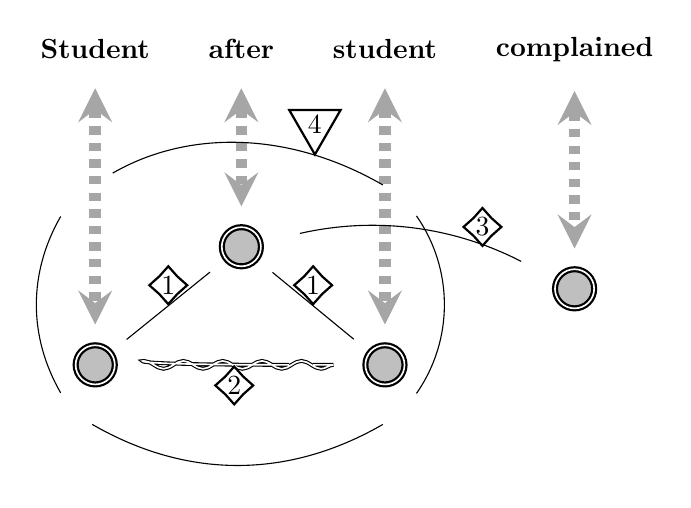
\begin{tikzpicture}

%\tikzset{snake it/.style={decorate, decoration=snake, segment length=5mm, amplitude=15mm}}

%\draw

%\node [s1] at (0,0) {Student};

\node (s1) at (1,1) {\textbf{Student}};
\node (after) [right=5mm of s1] {\textbf{after}};
\node (s2) [right=5mm of after] {\textbf{student}};
\node (complained) [right=5mm of s2] {\textbf{complained}};

\node (s1Rep) [double,draw=black,shape=circle,thick,fill=gray!50,inner sep=.5em,below=3.5cm of s1] {};
\node (afterRep) [double,draw=black,shape=circle,thick,fill=gray!50,inner sep=.5em,below=2cm of after] {};
\node (s2Rep) [double,draw=black,shape=circle,thick,fill=gray!50,inner sep=.5em,below=3.5cm of s2] {};
\node (complainedRep) [double,draw=black,shape=circle,thick,fill=gray!50,inner sep=.5em,below=2.5cm of complained] {};

\draw [ |-,-|, <->, line width = .8mm, draw=gray!70, 
 dashed, double equal sign distance, >= stealth, shorten <= .25cm, shorten >= .25cm ]
 (s1) to (s1Rep);

\draw [ |-,-|, <->, line width = .8mm, draw=gray!70, 
 dashed, double equal sign distance, >= stealth, shorten <= .25cm, shorten >= .25cm ]
(after) to (afterRep);
 
\draw [ |-,-|, <->, line width = .8mm, draw=gray!70,  
 dashed, double equal sign distance, >= stealth, shorten <= .25cm, shorten >= .25cm ]
(s2) to (s2Rep);

\draw [ |-,-|, <->, line width = .8mm, draw=gray!70, 
 dashed, double equal sign distance, >= stealth, shorten <= .25cm, shorten >= .25cm ]
(complained) to (complainedRep);
 
\draw [shorten <= .25cm, shorten >= .25cm ] 
(afterRep) to node [draw=black,shape = star,star points=4,thick,inner sep = 0mm, above] {1} (s1Rep);

\draw [shorten <= .25cm, shorten >= .25cm ] 
(afterRep) to node [draw=black,shape = star,star points=4,thick,inner sep = 0mm,above] {1} (s2Rep);

\node (s1E) [left=-2mm of s1Rep.east]{};
\node (s2E) [left=1mm of s2Rep.west]{};

\draw [shorten <= 2cm, shorten >= .3cm, double, % bend left = 5, 
decorate, decoration={snake, segment length=5mm, amplitude=.5mm}] %, amplitude=15mm]  
(s1E) to node [draw=black,shape = star,star points=4,thick,inner sep = 0mm, below] {2} (s2E);

\draw [shorten <= .5cm, shorten >= .5cm ] 
(afterRep) edge [bend left=20,looseness=1] node [draw=black,shape = star,star points=4,thick,inner sep = 0mm, 
 above, near end ] {3} (complainedRep);

\node (frameTopLeft) [below left = 1.5cm and -.65 cm of s1] {};
\node (frameBottomLeft) [below = 2.5cm of frameTopLeft] {};
\node (frameBottomRight) [right = 3.95cm of frameBottomLeft] {};
\node (frameTopRight) [above = 2.5cm of frameBottomRight] {};

\draw [shorten <= 0.15cm, shorten >= 0.15cm ] 
(frameTopLeft) edge [bend right=30,looseness=1] (frameBottomLeft);

\draw [shorten <= 0.15cm, shorten >= 0.15cm ] 
(frameBottomLeft) edge [bend right=30,looseness=1] (frameBottomRight);

\draw [shorten <= 0.15cm, shorten >= 0.15cm ] 
(frameBottomRight) edge [bend right=35,looseness=1] (frameTopRight);

\draw [shorten <= 0.15cm, shorten >= 0.45cm ] 
(frameTopRight) edge [bend right=30,looseness=1]
node [draw=black,shape = regular polygon,regular polygon sides=3,thick,inner sep = .2mm, 
above, near start, shape border rotate = 180] {4} (frameTopLeft);

%node [draw=black,shape = star,star points=4,thick,inner sep = 0mm, above, 
%bend left=100,looseness=3] {3}

%;


\end{tikzpicture}
\end{minipage}

\hspace{0.1\textwidth}
\begin{minipage}{0.8\textwidth}
			\renewcommand{\labelitemi}{$\blacklozenge$}
	
\begin{itemize}\setlength\itemsep{-.3em}
\item 1 \hspace{12pt}  Head/dependent relation
\item 2 \hspace{12pt}  Argument repetition ({}\BlankAfterBlank{} idiom)
\item 3 \hspace{12pt}  Propositional completion ({}\VisNtoS{})	
			\renewcommand{\labelitemi}{$\blacktriangledown$}
\item 4 \hspace{12pt}  Phrase (modeled as applicative structure), typed as {}\NPl{} 
\end{itemize}
\end{minipage}
\end{figure}
As this shows, the \q{Student after Student} idiom can be notated as, say,
\AfterNSingAndNSingToNPl{} (using \NSing{} and \NPl{} to mean singular
and count-plural nouns, respectively), but with the special case that the \q{argument} to
\i{after} is repeated in both positions, suggesting an unusual degree of repetition,
something frustratingly recurrent: \i{He went on and on}; \i{Car after car passed
us by}; \i{Time after time I got turned down}.
Although I have no problem
treating these constructions as idiomatic plurals, I also contend (on the
premise of phrase-overlap) that the dependent constituents in the \BlankAfterBlank{}
construction can be hooked to other phrases as well (which is why
\q{and [their/his/her] parents} can also be singular, in this case).  I dwell on
this example because it shows how type/functional accounts of phrase structure
can be useful even if we treat phrases more as frames which overlay linguistic
structure, not as rigid compositional isolates.  Each \q{students} variation uses
morphology to nudge cognitive attention in one direction or another, toward events or the
degree to which events are representative of some global property (here of
a student body), or both.  The \NSingToNPl{} transformation is not \i{the}
morphosyntactic meaning, but instead the skeleton on which the full meaning
(via cognitive schema) is designed, its hints solicited.
}
\p{If this analysis has merit, it suggests that a \CAG{}
approach to phrases like \i{many students} or \i{student after student}
(singular-to-plural or plural-to-plural mappings) should be understood not just
as functions among Part of Speech (\POS{}) types but as adding cognitive shading, foregrounding
or backgrounding cognitive elements like events or typicality in some context.
In other words, \i{many students} is type-theoretically \NtoN{} or \NpltoNpl{};
but, in more detail, it adds a kind of cognitive rider attached to the mapping which focuses
cognition in the subsequent discourse onto events (their recurrence and temporal distribution);
similarly \q{student after student} has a \q{rider} suggesting more of a temporal
unfolding.  The second form implies not only that many students complained, but that
the events of these complainings were spread out over some stretch of time.
Each such functional application (mappings between \POS{} understood as linguistic types)
produces not only a resulting \POS{} \q{type}, but also a reconfiguration of cognitive
attitudes toward the relevant situation and context.
Language users have many ways to craft a sentence with similar meanings, and arguably one
task for linguistic analysis is to model the space of choices which are available in a
given situation and represent what specific ideas and effects are invoked by one
choice over others.  It would be an argument in favor of Dependency Grammar if
Dependency-oriented representational models, like Link Grammar, prove to be
especially adept in this modeling.
}
\p{In this analysis, I am already switching to functional and type notions that will be
discussed in greater detail below; my current emphasis is on link grammar as a syntactic
conception, although I have also tried to argue that separating syntax from semantics
can be at most provisional.  Inter-word \q{link pairs} are vehicles for expressing
syntactic rules (like singular/plural agreement) but are also a ground level for
semantic analysis, since we can explain how semantic nuances are carried, in
specific sentences, by the actual link-pairs in evidence (violations to
agreement norms, for example).  These semantic nuances in turn can be given
cognitive interpretations, revealing the syntax-semantics-cognition pattern
which I am sketching here through specific perspectives like Link Grammar and
Type Theory.  Returning to the initial grammatic stage of analysis, however,
my tactics for contrasting overall Dependency and Phrase-Structure paradigms
rest on an implicit picture of how theories should be evaluated.
While such a picture is probably fairly consistent across perspectives, it is still worth
making a little more explicit.
}
\subsection{Explanation and Formality}
\p{Both Dependency and Phrase Structure grammars
presuppose that the fundamental exposition and achievement of their theory involves
formal transformation of linguistic givens, resulting in a more complex data structure
which, to the extent that the theory is correct and useful, models something
of the inner structure of language (\i{qua} abstract formal system and/or cognitive phenomenon).
The \q{data structure} might be a phrase-structure \q{tree} or a graph-like dependency
\q{linkage}, but while these representations have different form they share certain
criteria: they are formally describable systems which allow some structures but reject others;
they are rigorous enough to be given a mathematical (e.g., algebraic) definition;
and they can be expressed in computer code which builds these structures out of
Natural Language artifacts, can verify that an instance of the relevant data structures
satisfies the system rules, and can execute operations which modify the structures.
The phrase trees or word-link graphs are \q{formal substrata} which encapsulate Natural Language
patterns but also are rigidly mathematical and computational.  How thoroughly these substrata
capture linguistic meaning, is therefore directly relevant to questions of whether and
in what degree natural language itself, as social and cognitive, is also formal and computational.
}
\p{Translating NL content into (say) a linked-grammar graph does not make software capable
of \q{understanding} language.  If Dependency Grammar is a reasonable foundation
for linguistics in general, then properly parsing sentences into their
auxiliary graphs is, at most, a step in the direction toward \q{understanding}.
Even this may beg the question of what constitutes a \q{correct} parse: when writing
real-world code, language engineers appear to rely principally on their own intuitions, based
on their familiarity with the underlying theory, the idea they have of what a
\i{correct} \q{re-presentation} looks like (for link grammar, of the correct collection of
link types between the various words).  They then add code to ensure that this representation
is indeed identified by the software in specific examples, and try to do so in such a way
as to generalize to other examples.  This methodology can be gleaned from observing internet chat
sites and other informal research venues; one can witness developers painstakingly constructing
systems which \q{work right} in the sense of producing the interpretation for each sentence
which corresponds with what the human linguists perceive, even for sentences which the
software has never encountered before.  The code is considered reliable the more that
new sentences are \q{correctly} parsed.  Again, \q{correctly} here means, conformant to
linguists' own interpretations; insofar as these are subjective, such conformance is not
conclusive evidence that the transformational algorithms are \q{correct}.
}
\p{In order to assess linguistic \q{competence} (or whatever computational ability may simulate it),
it is needed to check specific \q{behavior} and compare it to some expectation.  The gold standard
for linguistic behavior is just participating in a linguistic community, judged by the community
at large as fully competent and included.  Unfortunately, however \mdash{} at least for those who
want to profit from Artificial Intelligence \mdash{} achieving true \q{language-like behavior} may be
impossible.  Scholarship therefore has to turn toward more limited notions of
competence, such as representational transformation of sentences \mdash{} but since
each theory has its own picture of what sentences should be transformed \i{into},
the justification of competence measures can be circular.  It is the theory which
dictates how the software should act, and the software is deemed \q{intelligent} if it
acts accordingly.  We can be skeptical of such non-theory-neutral conceptions of
\q{intelligence}.  Nonetheless it does count
in theories' favor if they both propose accounts of language structure which
are independently defensible and also can produce computing systems that
reliably and without external direction map language onto those structures.
Language-like behavior then involves producing a transformed representation of
language embodying a particular theoretical conception of
linguistic \q{deep structure}.
}
\p{It would serve Computational-Linguistic theories still further to create systems
that demonstrate behavior which is \q{language-like} on terms less wedded to their
own hypotheses.  More satisfying definitions of linguistic behavior would involve intuitions
of language users in general, not just language experts.  For example, document classifiers
\mdash{} which typically use statistical analysis to predict which topic will be deemed most
relevant for documents like news stories and technical articles \mdash{} again illustate a kind
of transformational representation, converting Natural Language to a formal data structure
(in this case a relatively simple one, naming one or multiple topics from a predefined list).
In this case however a broad user public can provide feedback on how well the system performs.
For another example, artificial translators map language onto formal structures but then
attempt an opposite map, translating the formalized representation into natural-seeming
expressions in a different language.  This case is different in that formal representation is
an intermediary rather than end point of the transformation, but like document classifiers it
is a kind of behavior whose effectiveness can be judged by a large community of speakers.
People who interact with text \q{chat} bots, or talking robots, and feel that the experience
is similar to talking with another person, are also providing evidence of more complete and
larger-scale language-like behavior.  Again, though, it is not now and may never be possible
to engineer intelligent behavior to this level of perfection.  Existing language \AI{} platforms
are flawed but useful, which suggests both that formal re-presentation is an important
step toward language understanding but also that attempts to use these formalisms as a springboard
to more holistic behavior \mdash{} like automated translation, but also extracting practical
information, or gleaning emotion and sentiment \mdash{} are missing something essential.
Doing useful things with or gleaning useful insight from the re-presentational target structures
appears to be a separate problem from that of generating them \mdash{} which calls into question the
degree to which the target structures sufficiently encapsulate linguistic meaning,
even if they reveal structures which are essential to linguistic meaning.
}
\p{This does not have to mean that Natural Language Processing is basically impossible, only
that more modest criteria of \q{correct} \NLP{} systems need to be adopted.  This is complicated
by the fact that artifical language behavior can be flawed but meaningful: \q{Urine shift one
step forward} is an awkward English sentence but its meaning seems clear enough
(this real example comes from a shopping center in New York's Flushing, Queens Chinatown).
We have an intuition that some expressions are \q{incorrect} but not so completely
off-base that they fail to signify anything at all \mdash{} but in this case we need
criteria for how a linguistic performance can be both incorrect \i{and} nonetheless coherent.
}
\p{These issues influence any theory which approaches linguistic competence from the
viewpoint of formal re-presentations, and therefore effectively all branches of
Computational Linguistics.  The reigning assumption appears to be that transformational
representation which converts language to theory-regulated data structures, for which
in many cases the transformation achieved by mechanical algorithms matches that
intuited as most accurate by human experts, serves as \i{prima facie} evidence of
something like computationally-engineered  \q{intelligent (language) behavior}.
This leaves room for language-like behavior to productively replicate dimensions
of language understanding while also being very incomplete: language-like relative
to experts' opinions on deep linguistic structure, not real-world communication.
Structures like link grammar graphs can be essential formal substrata that linguistic expression
relies on to achieve communication, without being the sole medium of this expression.
}
\p{My arguments so far have used Link Grammar as a representative example
of \q{transformational representation} where a computational system
can be judged to reveal some level of language competence, some
kind of \q{language like behavior}, insofar as it translates natural
language expressions to data structures conformant to Dependency
Grammar (and particularly Link Grammar) theory.
As I also just argued, performance \visavis{} structural transformation
may be only tangential to human language, so whatever theory is
built up needs a separate, more philosophical or metatheoretical analysis
to consider how the theory is purported to engage with its phenomena.
But I now take this as a starting point for pivoting the discussion from
grammar to semantics; and will defer until after that speculating
on philosophical implications of the theory thus extended.
}

\section{Cognitive Grammar and Type Theoretic Semantics}
\p{The emergence of Dependency Grammar as a \i{computational} approach has some broad
implications.  The historical preference for phrase-structure foundations  \mdash{} among
those who actually build Natural Language Processing code libraries, in disciplines
related to Artifical Intelligence \mdash{} arguably reflects how phrase structure more
cleanly models a theory of linguistic meaning and signification based on
\q{symbolic logic} \mdash{} a theory that the \i{meaning} of a complete and self-contained
linguistic expression is the logical state of affairs which it asserts or in other
ways connotes.  Correlated with this assumption is the idea that phrase structure
logically transforms its constituent parts; so from the word \q{students} we
can form the phrase \q{many students} to designate a kind of plurality \mdash{} a plural
set but also, more specifically, a set which is reasonably large relative to some context.
In the hierarchical model presented by these norms, phrases subsume the roles of
individual words and represent discrete semantic units with respect to still larger phrases.
}
\p{It is certainly true that one role for phrases is to satisfy a semantic niche \mdash{} often
a place occupied in other (or even the same) language with single words, or vice-versa.
The French \q{laisse tomber} translates the English \q{drop}, for example; and
\q{parliamentarian} is a more exotic version of \q{Member of Parliament}.  There is no
evident pattern for when a single concept is conveyed, in one language or another,
by a single word or a multi-word phrase.  Moreover, the meanings of phrases are influenced
by semantic conventions no less than are individual words, and they are not solely a product
of phrase constituents.  Semantics is guided by what people need to talk and write about often; when
events in a linguistic community call for some fairly rigid and repeatable designation for
an important concept, the resources of language adjust to provide that role, either through a
complete neologism, or a lexical variant \mdash{} a new usage; or the entrenchment of a phrase.
In current events, the expression \q{Syrian Refugees} recurs when discussing people
displaced by the Syrian civil war, and potentially other interrelated conflicts also;
convention seems to allow that nominal \q{Syrian} Refugees don't have to be Syrian nationals.
The meaning of the phrase is fixed by its niche in familiar discourse more than
by its literal form.  Phrases
exhibit conventionalization and usage pressures analogous to single words; which lends
credance to the notion that phrases subsume the role of single words, and that the semantic
contribution of words to sentences is determined through the phrases where they occur.
}
\p{On the other hand, it is well established that words' contributions are not \i{wholly}
subsumed by their surrounding phrase-structure.  The famous joke about the Holy Roman
Empire \mdash{} or its reprise in the current line that the Islamic State is neither Islamic
nor a State \mdash{} point to evidence that as language-users we still hear the individual
words outside their phrase context.  To subsume a word into a phrase is also to suggest a
particular semantic (and pragmatic, real world) interpretation, one which conversants
may challenge.\footnote{How literally to take phrases is a notorious source of political controversy:
recall debates about the relevance of Afghanistan for Iraq, in US policy, and
Rudy Giuliani saying \q{There \i{is} Al Qaeda in Iraq \mdash{} it's called, \sq{Al Qaeda in Iraq}}.
}
}
\p{Arguably, joking or titular cases like \q{Holy Roman Empire} can be
relegated to thematic margins, especially if we accept formal-logical construals of
what semantics is all about, with an \i{a priori} contrast between Semantics and
Pragmatics, the former rooted in \i{states of affairs} and only the latter addressing
rhetoric and usage.
Counter to this counter-argument, however, we can observe that different phrases imply
different degrees of \q{autonomy} to their constituents, and different degrees of
coherence or unification into a single idea.  Some phrases act as direct substitutes
for single concepts (like \q{Member of Parliament}) where it seems mostly historical
accident that a phrase rather than a word emerged as the most popular; but many other
phrases have more complex usage scanarios, including everyday expressions that don't have
special rhetorical or sociolinguistic conventions that would make them tangential to
semantic or syntactic analysis proper.  Moreover, many of these examples are similar to
those used by Cognitive Grammar to challenge the syntax/semantic distinction and argue for
\q{morphosyntactic} models as reciprocating cognitive formations, not abstract language-rules.
}
\p{For example, in Ronald Langacker's \i{Foundations of Cognitive Grammar}, the sentence
\begin{sentenceList}\sentenceItem{} Three times, students asked an interesting question
\end{sentenceList}
is used to demonstrate how
grammatical principles follow from cognitive \q{construals} of the relevant situations,
those which language seeks to describe or takes as presupposed context.\footnote{For example, \cite[pp. 119 and 128]{LangackerFoundations},
discussed by \cite[p. 189]{LineBrandt}, and \cite[p. 9]{EstherPascual}.
}
In particular, Langacker argues that \q{students} and \q{question} can both be either singular or
plural: syntax is open-ended here, with neither form more evidently correct.  Langacker uses this
example to make the Cognitive-Linguistic point that
we assess syntactic propriety relative to cognitive frames and conversational context.  In this
specific case, we are actually working with two different cognitive frames which are interlinked
\mdash{} on the one hand, we recognize distinct events consisting of a student asking a question, but
the speaker calls attention, too, to their recurrence, so the events can also be understood
as part of a single, larger pattern.  There are therefore two different cognitive foci, at two
different scales of time and attention, a \q{split focus} which makes both singular and plural
invocations of \q{student} and \q{question} acceptable.
}
\p{Supplementing this analysis, however, we can additionally focus attention directly on
grammatical relations.  The words \q{student} and \q{question} are clearly linked as the subject and
object of the verb \q{asked}; yet, contrary to any simple presentation of rules,
no agreement of singular or plural is required between them (they can be singular and/or plural in
any combination),  Moreover, this anomaly is only in force due to the context established
by an initial phrase like \q{Three times}; absent some such framing, the singular/plural
relation would be more rigid.  For example, \q{A student asked interesting questions} would
(in isolation) strongly imply \i{one} student asking \i{several} questions.  So the initial
\q{Three times} phrase alters how the subsequent phrase-structure is understood while remaining
structurally isolated from the rest of the sentence.  Semantically, it suggests a
\q{space builder} in the manner of Gilles Fauconnier or Per Aage Brandt
\cite{Fauconnier}; \cite{PerAageBrandt}, but we
need to append Mental Space analysis with theory of how these spaces
influence syntactic acceptability, which would seem to be logically prior to the stage where Mental Spaces
would come in play.  This complex interplay of phrase-structures
is hard to accommodate from the grammar-hierarchy perspective.  There seems to be
no way to break down this example sentence into a tree-like phrase hierarchy wherein each
phrase, considering the semantic concept which it is apparently tasked to put into words,
can be seen to function in isolation.  The mapping of the sentence to a logical
substratum would be more transparent with a sentence like \q{Three students asked
interesting questions}; that sentence is a more direct translation of the facts
which the original sentence conveys.  But this \q{more logical} sentence has different
connotations than the sentence Langacker cites; the original sentence places the emphasis
elsewhere, calling attention more to the idea of something temporally drawn-out,
of a recurrence of events and a sense of time-scale.  The \q{more logical} sentence
lacks this direct invocation of time scale and temporal progression.
}
\p{We can say that the \q{Three students} version is a more direct statement of fact, whereas
Langacker's version is more speaker-relative, in the sense that it elaborates more
on the speaker's own acknowledgment of belief.  The speaker retraces the steps of her
coming to appreciate the fact \mdash{} of coming to realize that the \q{interesting questions}
were a recurrent phenomenon and therefore worthy of mention.  By situating expression
relative to cognitive process rather than to the facts themselves, the sentence
takes on a structure which models the cognition rather than the states of affairs.
But this shift of semantic grounding from the factual to the cognitive also apparently
breaks down the logical orderliness of the phrase structure.  \q{Three times}, compared
to \q{three students}, leads to a morphosyntactic choice-space which is
\q{underdetermined} and leaves room for speakers' shades of emphasis.
}
\p{This is not an isolated example.  Many sentences can be provided with similar
phrase-structure complications, particularly with respect to singular/plural agreement.
\begin{sentenceList}\sentenceItem{} Time after time, tourists (a tourist) walk(s) by this building
with no idea of its history.
\sentenceItem{} The streets around here are confusing; often people (someone)
will ask me for directions.
\sentenceItem{} Student after student came with their (his/her)
paper to compain about my grade(s).
\sentenceItem{} Student after student \mdash{} and their (his/her) parents
\mdash{} complained about the tuition increase.
\end{sentenceList}
On a straightforward phrase-structure reading, \q{Student after student} reduces to an
elegant equivalent of \q{Many students}, with the rhetorical flourish abstracted away
to a logical form.  But our willingness to accept both singular and plural agreements
(his/her/their parents, grades, papers) shows that clearly we don't simply substitute
\q{Many students}; we recognize the plural as a logical gloss on the situation but
engage the sentence in a more cogntively complex way, recognizing connotions of temporal
unfolding and juxtapositions of cognitive frames.  The singular/plural underdeterminism
is actually a signification in its own right, a signal to the listener that the
sentence in question demands a layered cognitive attitude.  Here again, syntactic
structure (morphosyntactic, in that syntactic allowances are linked with
variations in the morphology of individual words, such as singular or plural form)
serves to corroborate conversants' cognitive frames rather than to model logical
form.
}
\p{This is not to say that phrase-structure paradigms are refuted by these examples.  Cases
like these can be accommodated by layering new structural rules, such as
allowing exceptions for singular/plural agreement in the presence of certain
\q{lead-in} phrases like \q{Three times}.  It is not even accepted that these
examples clearly favor inter-word relations (as language formalization, in preference over
phrase-structure trees) \mdash{} cases like \q{Student after student} have
also been used \i{against} Dependency Grammar on the argument
that there is not a clear \q{single} word, in that phrase,
which should be seen as linking with words elsewhere in the sentence
\cite[pp. 400-401]{MullerBook}, \cite[p. 2]{MullerPDF}.  It
seems arbitrary to select either \q{student}, or \q{after}, as \q{the}
representative of the phrase to link with \mdash{} for example \mdash{} the verb
\q{complained}; on that argument, the least arbitrary analysis is to
treat the phrase as a whole as a single unit for purposes of grammatic
linkage.  In short, both paradigms have potential problems with these example.
Considering \q{Student after student} as an encapsulated phrase leaves
the singular/plural flexibility in the continuation of the sentence unexplained
(\q{Many students compained about \qmarkdubious{}his grade} is clearly dubious, so
\q{Many students} is not a direct substitution). But bracketing the phrase
when decribing the sentences' \q{linkage} leads
to an apparently arbitrary choice when it comes time to notate the subject/verb
linkage for \q{complained}.  I will address this particular ambiguity later;
but for now I'll just point out that a simplistic reading of
both Dependency and Phrase-Structure ideas seems to run aground.
}
\subsection{Comparing paradigms}
\p{Since Computational-Linguistic paradigms find practical expression in code
libraries, there are some options to assess competing theories empirically
\mdash{} comparing libraries' speed, accuracy, ease of use, and how readily can they be
modified in light of new research.  Arguably, however, the
quality of a code library does not automatically reflect the accuracy of
its underlying linguistic paradigms (as opposed to the skill, foresight, and
resources of its programmers); not to mention that more complex analyses of
human language may be both more correct and also harder to express in code.
There is, in any case, no apparent consensus amongst linguists and programmers that one
or another language theory has proven computationally preferable.  Another approach to
theory-comparison involves considering the range of linguistic phenomena which different methods can explain, without resorting to ad-hoc compilations of exceptions and
special cases.  Arguably, here, Dependency Grammar provides more
straghtforward explanations.  For example, the internal structure of phrases seems to
lend specificity and nuance to their meaning in ways that get lost when
trying to replace phrases with logico-semantic equivalents.
\q{Student after student} is not losslessly substitutable with \q{Many students},
and the former phrase has a temporal and multi-tier cognitive implication which
the latter discards.  The second phrase is compatible with \q{Many students}
complaining \i{at one time}, as well as drawn out over time; the former phrase
appears to clarify that the second kind of situation is the intended meaning,
Of course, in context, the two phrases may be understood to have similar meanings;
but this is a product of how the linguistic structure relates to its presumptive
conversational context, not to an intrinsic semantic equivalence.  I will
now consider these and other examples to discuss the dependency/phrase-structure
contrast in a little more detail.
}
\p{The contrast between the phrases \q{Student after student} and \q{Many students}
cannot be based on \q{abstract} semantics alone \mdash{} how the evident temporal implications of the
first form, for example, are concretely understood, depends on conversants' mutual recognition
of a relevant time frame.  The dialog may concern a single day, a school year, many
years.  We assume that the speakers share a similar choice of time \q{scale}
(or can converge on one through subsequent conversation).  \i{Some} time-frame
is therefore presupposed in the discursive context, and the first phrase invokes
this presumed but unstated framing.  The semantics of the phrase are therefore somewhat open-ended:
the phrase \q{hooks into} shared understanding of a temporal cognitive framing without referring
to it directly.  By contrast, the second phrase is less open-ended: it is consistent with both
a more and less temporally protracted understanding of \q{many}, but leaves such details (whatever
they may be) unsignified.  The factual circumstance is designated with a level of abstraction that sets
temporal considerations outside the focus of concern.  The second phrase is therefore both
less open-ended and also less expressive: it carries less detail but accordingly also relies
less on speaker's contextual understanding to fill in detail.
}
\p{Clearly the two phrases are therefore semantically different; but notice also that the
semantic properties of the first phrase are due explicitly to its internal structure.
The temporality implicatures could be expressed in a more \q{purely} semantic
fasion with a choice of wording, like \q{a procession of students complained}.  This
would rely on the conventional meaning of \q{procession} (or \q{stream}, \q{sequence},
etc.) to provide the expressive \q{time} dimension.  But the \q{Student after student}
phraseology achieves this effect more economically and with more \q{oomph} because the
internal repetition in the phrase itself effectively models the recurrence it
seeks to feature semantically.  Here linguistic form actually does reproduce
factual structure, like a syntactic version of onomatopoeia.  This fact of internal structure
clearly can only be fully modeled by taking seriously the exact composition of the phrase, not
treating the phrase-structure as a convention fully subsumed by a semantic role.
}
\p{In addition, aside from the expressive detail which depends on the actual phrase
structure (which therefore cannot be summarized away), this inner structure also
governs morphosyntactic possibilities over all.  \q{A procession of students}
captures a similar temporal progression but also fully absorbs \q{student} in a plural
guise, and \q{A procession of students complained about \qmarkdubious{}his grade} is straightforwardly
ungrammatical.  In Langacker's \q{Three times} example, the inter-word
\q{linkage} captures the aforementioned complexities in a reasonably non-arbitrary
way, I believe.  \q{Student} is linked as subject-to-verb with \q{asked}, and as
subject-to-object with \q{question}.  It is true that these link-pairs seem to
violate agreement norms, but there is nothing in the Link Grammar paradigm \mdash{} which
practices Dependency Grammar with a rather detailed and intricate
inventory of inter-word relations, or \q{links} \mdash{} mandating that
\i{all} link-pairs exhibit forced agreement (like singular/plural).  Agreement, when it
applies, is a property \i{of} link pairs.  There is also an implicit
(cross-phrasal) link between \q{student} and \q{Three} \mdash{} clarifying that, considered
in its entirely, the sentence is about three students precisely \mdash{} and the presence of
this kind of link alters how the other links connecting to the word \q{student} are
assessed.  In particular, this latter link stipulates that the word \q{student} is being
simultaneously understood in both a plural and a singular sense, so it permits
singular \i{and} plural link forms which, more commonly, could only be
singular \i{or} plural.  So link grammar can offer an elegant analysis of
singular/plural \q{underdeterminism}, expressed in the
same underlying graph-context terminology as most other link-grammar theorizing.
It would be unfair to use this as a case against Phrase Structure grammars without a
detailed presentation of how these grammars would handle such a case in turn, but
I'd argue that link grammar accommodates this complex example with relatively little
departure from its underlying theoretical and notational or presentational commitments.
}
\p{While my previous examples contrasted Phrase Structure and Dependency
Grammars in terms of their resources for explaining sentences with
unusual semantic patterns but relatively clear meanings (in context),
another form of comparison can address actual ambiguity.  Consider
\begin{sentenceList}\sentenceItem{} The Maple Leafs failed to win in overtime for the
first time this year.
\sentenceItem{} The Maple Leafs failed for the first time this year
to win in overtime.
\end{sentenceList}
The first can mean either that the Leafs had won \i{all} or \i{none}
of their prior overtime games.  From a phrase-structure perspective,
we have to image that \q{to win in overtime} can \q{migrate} so we
hear it as in the second version of the sentence.  For more inter-word
grammars, the alternation is simpler: \q{for}, initiating the phrase
\q{for the first time}, can be linked with either \i{failed} or
\i{win} \mdash{} notationally, it amounts to the presence or absence of one
graph-edge, when the syntax is represented as a graph with
inter-word labels for link kinds.  This could be a distinction without
a real difference, since choosing which inter-word link to recognize
triggers linking in the rest of the phrase along with it.
But perhaps reflecting on how we process the ambiguity \mdash{} realizing
that there are two competing parses and deciding which is the one
intended \mdash{} we picture the alternatives more as \q{horizontal}
options for connecting threads across the sentence,
more so than a \q{vertical} organization where
we hear \q{for the first time} as \q{contained} in a larger phrase.
My own feeling is of exploring competing relational patterns more than
exploring different ways that the phrases can be nested inside each
other.
}
\p{That being said, how much of our sense of ambiguity (or clarity, for
that matter) is driven by meaning, not form?  The \q{double parse}
just examined does not always generalize to similar cases:
\begin{sentenceList}\sentenceItem{} The Maple Leafs failed to win two consecutive games
for the first time this year.
\end{sentenceList}
The reading as in \q{this is the first time they failed to win two
consecutive games} makes no sense \mdash{} unless you've won every game,
but perhaps the first, you've at some point lost after a win.  Is this
case anomalous, where a syntactic ambiguity idiosyncratically fails to
yield logically plausible readings?
The ambiguity is found in \i{failed to make the playoffs
for the first time since 2013}, and many \i{for the first time this
season} cases, like \i{beat the Habs}, \i{sell out the arena},
\i{score a goal in the first period}.  But \q{failed to score a goal}
is almost surely read that they \i{did} score in every prior game.
Do we hear the construction as intrinsically ambiguous, and reject one
reading only when it is clearly flawed pragmatically?
}
\p{If we believe that language understanding unfolds in a predictable
operational sequence, then we should assume that both parses are
deemed plausible, and semantic considerations only retroactively
eschew one reading (if they do so at all).  This would explain why in
many cases the ambiguity persists enough to cast the practically
intended meaning in doubt.  But that account does not consider the
temporality of language itself; the hearer does not know in advance
that a trailing phrase like \q{for the first time this season} is coming,
and starts to make sense of the sentence up to there; once then hearing or
reading the addendum, the audience instinctively has to interpret the
final phrase as deliberately inserted to modify an already-complete
idea.  On this analysis, the addendum is initially approached as a
performative detail, something said for a reason to be determined \mdash{}
it is not structurally necessary to make the sentence well-formed.
Perhaps we then try to fit the last phrase into the sentence both
syntactically and semantically, together, triggered by a pragmatic
phenomenon (the speaker's choice to add on to a seemingly complete
thought) which then becomes logically prior to both syntax and
semantics.  If this is plausible, it supports an inter-word relational
model because we are forming a picture of language structure
relationally, assimilating new words and phrases to those already
heard by linkings referring back in time, rather than waiting until we
are sure we have a complete sentence and then treating it as a static
structure to vertically reconstruct.
}
\p{The examples I have used so far may also imply that a choice of phrase structure is
always driven by semantic connotations of one structure or another;
but seemingly the reverse can happen as
well \mdash{} speakers choose a semantic variant because its grammatic realization lends a useful
organization to the larger expression.  There are many ways to say \q{many},
for example: \i{a lot of},
\i{quite a few}, not to mention \q{time after time} style constructions.  Whatever their
subtle semantic variations, these phrases also have different syntactic properties:
\i{Quite a few} is legitimate as standalone (like an answer to a question);
\i{A lot of} is not, and \i{A lot} on its own is awkward.  On the other hand the \q{of} in
\i{A lot of} can \q{float} to be replicated further on: \q{A lot of students, of citizens,
believe education must be our top priority} sounds more decorous than the equivalent sentence with the
second \q{of} replaced by \q{and}.  If the cadence of that sentence appeals to the speaker, then
such stylistic preference will influence taking \q{A lot of} as the \q{many} variant of choice.
So speakers have leeway in choosing grammatic forms that highlight one or another aspect of
situations; but they also have leeway in choosing rhetorical and stylistic pitch.  Both cognitive
framings and stylistic performance can be factored when reconstructing what compels the
choice of one sentence over alternatives.
}
\p{One consequence of these analyses, should they be accepted, is that grammar
needs to be approached holistically: the grammatic structure of phrases cannot,
except when deliberate oversimplification is warranted, be isolated from
surrounded sentences and still larger discourse units.  Semantic roles
of phrases have some effect on their syntax, but phrases are nonetheless chosen
from sets of options, whose variations reflect subtle semantic and syntactic
maneuvers manifest at super-phrasal scales.  The constituent words of phrases retain some
autonomy, and can enter into inter-word and phrasal structures with other words outside their
immediate phrase-context.  We can still apply formal models to phrase
structure \mdash{} for example, Cognitive and Applicative Grammar (\CAG{}) considers phrases
as \q{applications} of (something like) linguistic or cognitive \q{functions},
in the sense that (say) an adjective is like a \i{function} applied to a noun,
to yield a different noun (viz., something playing a noun's conceptual role)
\cite{Descles2010}.
I will consider related \q{functional} and (by extension) Type-Theoretic
approaches in the next section.  But we should not read these transformations
\mdash{} like \i{Syrian refugee} from \i{refugee} \mdash{}
too hastily as a purely semantic correlation within a space of denotable concepts
\mdash{} \i{such that} the new concept wholly replaces the
contained parts, which then cease to have further linguistic role and effect.
Instead, applicative structures represent shifts or evolutions in
mental construal, which proceed in stages as conversants form
cognitive models of each others' discourse.  Even if phrase structure
sets landmarks in this unfolding, phrases do not wholly subsume their
constituents; the parts within phrases do not \q{vanish} on the higher scale,
but remain latent and may be \q{hooked} by other, overlapping phrases.
This argument rests on a vantage point from semantics as well as syntax;
therefore, I will discuss it briefly at present (I return to
this analysis at greater length in the next section).
}
\p{Consider the effect of \q{Many students complained}.  Propositionally, this appears
to say essentially that \i{students} complained; but, on hermeneutic charity, the
speaker had \i{some} reason to say \q{many}.  The familiar analysis is that
\q{many} suggests relative size; but this
is only half the story.  If the speaker chose merely \i{students complained}, we would hear an assertion
that more than one student did, but we would also understand that there were several
occasions when complaints happened.  Adding \q{many} does not just
imply \q{more} students, but suggests a mental shift away from the particular episodes.
In the other direction, saying \i{a student complained} is not just
asserting how at least one student did so, but
apparently reports one specific occasion (which perhaps the speaker wishes to
elaborate on).  In other words, we cannot really capture the singular/plural semantics,
or different varieties of plural, just by looking at the relative size of implied
sets; we need to track how representations of singleness or multitude imply
temporal and event-situational details.  So \i{a student complained} focuses not
on the numeric count of one, but on a singular event (unlike
\q{\i{only one} student complained}); \i{students complained} focuses not on the
plural measure of students involved, but on the fact that a certain type
of event happened several times.  \i{Many students complained}
focuses not on sheer number (unlike \i{a large number of students complained}),
but rather on the implication that complaints were widespread enough to represent
a significant sample, perhaps a majority sentiment, among the student body.
The semantics of the former two forms seems to focus attention
on the \i{events} of complaining, while the \i{many students} construction seems
to focus more on their suggesting a prevailing attitude.  \q{Students complained}
seems to single out each event as distinct, even though there are several of
them; whereas \i{Many students complained} seems to construe the
events as each resembling the other, to the point where they partly
lose their individuality.  \q{Isolated events},
in the English idiom, are those which are atypical; as we cognitively
shift from the events as discrete to recurring patterns, they become
suggestive of a larger state of affairs.  By implication, if many students
complained, many other students may be unhappy; the extent of students'
unrest is no longer measurable by the multiplicity of the complaining-events.
}
\p{Against this backdrop, \i{Student after student complained} captures both dimensions,
implying both a widespread unrest among the student body and also
temporal recurrence of complainings.
Formal models of syntax and semantics often borrow notation from formal
language theory; for example, notations for Parts of Speech lifted
from functional programming languages.\footnote{A note on notation: I adopt the Haskell convention (referring to the Haskell
programming language and other functional languages) of using arrows both between
parameters and before output notation, but for visual cue I add one dot above the
arrow in the former case, and two dots in the latter: \argsToReturn{}.
I use \N{} for the broadest designation of nouns (the broadest
noun type, assuming we are using type-theoretic principles),
with extra markings for more specific types (in principle
similar notation could be adopted for verbs, propositions, and so on).
}
This notation can help us picture the \q{flow} of ideas building up
to a complete sentence, formally represented via type theory
(where sentences reveal a type hierarchy culminating in a self-contained idea,
that is, a proposition); more informally we can picture a similar
\q{conceptual} flow tracing how listeners come to make sense of the
language they encounter enunciated by speakers.  By way
of illustration, Figure ~\ref{fig:ESA} shows a
Depency-style descructuring, with implicit type annotations.  \begin{figure}
\caption{Dependency-style graph with argument repetition}	
\label{fig:ESA}
\vspace{1em}
\hspace{0.15\textwidth}	
\begin{minipage}{0.7\textwidth}
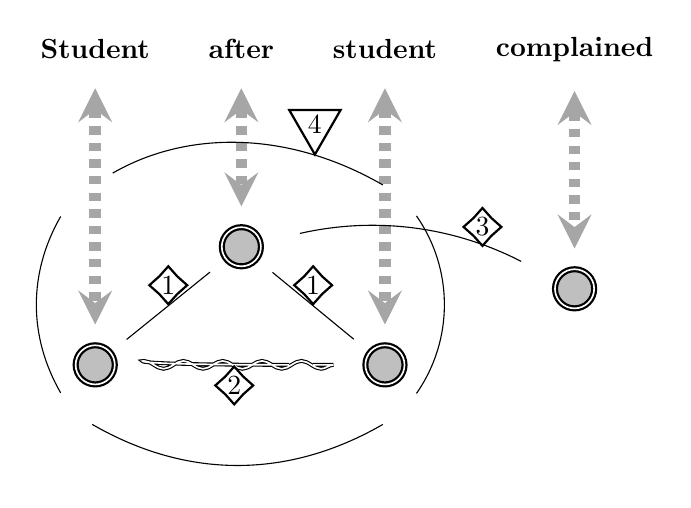
\begin{tikzpicture}

%\tikzset{snake it/.style={decorate, decoration=snake, segment length=5mm, amplitude=15mm}}

%\draw

%\node [s1] at (0,0) {Student};

\node (s1) at (1,1) {\textbf{Student}};
\node (after) [right=5mm of s1] {\textbf{after}};
\node (s2) [right=5mm of after] {\textbf{student}};
\node (complained) [right=5mm of s2] {\textbf{complained}};

\node (s1Rep) [double,draw=black,shape=circle,thick,fill=gray!50,inner sep=.5em,below=3.5cm of s1] {};
\node (afterRep) [double,draw=black,shape=circle,thick,fill=gray!50,inner sep=.5em,below=2cm of after] {};
\node (s2Rep) [double,draw=black,shape=circle,thick,fill=gray!50,inner sep=.5em,below=3.5cm of s2] {};
\node (complainedRep) [double,draw=black,shape=circle,thick,fill=gray!50,inner sep=.5em,below=2.5cm of complained] {};

\draw [ |-,-|, <->, line width = .8mm, draw=gray!70, 
 dashed, double equal sign distance, >= stealth, shorten <= .25cm, shorten >= .25cm ]
 (s1) to (s1Rep);

\draw [ |-,-|, <->, line width = .8mm, draw=gray!70, 
 dashed, double equal sign distance, >= stealth, shorten <= .25cm, shorten >= .25cm ]
(after) to (afterRep);
 
\draw [ |-,-|, <->, line width = .8mm, draw=gray!70,  
 dashed, double equal sign distance, >= stealth, shorten <= .25cm, shorten >= .25cm ]
(s2) to (s2Rep);

\draw [ |-,-|, <->, line width = .8mm, draw=gray!70, 
 dashed, double equal sign distance, >= stealth, shorten <= .25cm, shorten >= .25cm ]
(complained) to (complainedRep);
 
\draw [shorten <= .25cm, shorten >= .25cm ] 
(afterRep) to node [draw=black,shape = star,star points=4,thick,inner sep = 0mm, above] {1} (s1Rep);

\draw [shorten <= .25cm, shorten >= .25cm ] 
(afterRep) to node [draw=black,shape = star,star points=4,thick,inner sep = 0mm,above] {1} (s2Rep);

\node (s1E) [left=-2mm of s1Rep.east]{};
\node (s2E) [left=1mm of s2Rep.west]{};

\draw [shorten <= 2cm, shorten >= .3cm, double, % bend left = 5, 
decorate, decoration={snake, segment length=5mm, amplitude=.5mm}] %, amplitude=15mm]  
(s1E) to node [draw=black,shape = star,star points=4,thick,inner sep = 0mm, below] {2} (s2E);

\draw [shorten <= .5cm, shorten >= .5cm ] 
(afterRep) edge [bend left=20,looseness=1] node [draw=black,shape = star,star points=4,thick,inner sep = 0mm, 
 above, near end ] {3} (complainedRep);

\node (frameTopLeft) [below left = 1.5cm and -.65 cm of s1] {};
\node (frameBottomLeft) [below = 2.5cm of frameTopLeft] {};
\node (frameBottomRight) [right = 3.95cm of frameBottomLeft] {};
\node (frameTopRight) [above = 2.5cm of frameBottomRight] {};

\draw [shorten <= 0.15cm, shorten >= 0.15cm ] 
(frameTopLeft) edge [bend right=30,looseness=1] (frameBottomLeft);

\draw [shorten <= 0.15cm, shorten >= 0.15cm ] 
(frameBottomLeft) edge [bend right=30,looseness=1] (frameBottomRight);

\draw [shorten <= 0.15cm, shorten >= 0.15cm ] 
(frameBottomRight) edge [bend right=35,looseness=1] (frameTopRight);

\draw [shorten <= 0.15cm, shorten >= 0.45cm ] 
(frameTopRight) edge [bend right=30,looseness=1]
node [draw=black,shape = regular polygon,regular polygon sides=3,thick,inner sep = .2mm, 
above, near start, shape border rotate = 180] {4} (frameTopLeft);

%node [draw=black,shape = star,star points=4,thick,inner sep = 0mm, above, 
%bend left=100,looseness=3] {3}

%;


\end{tikzpicture}
\end{minipage}

\hspace{0.1\textwidth}
\begin{minipage}{0.8\textwidth}
			\renewcommand{\labelitemi}{$\blacklozenge$}
	
\begin{itemize}\setlength\itemsep{-.3em}
\item 1 \hspace{12pt}  Head/dependent relation
\item 2 \hspace{12pt}  Argument repetition ({}\BlankAfterBlank{} idiom)
\item 3 \hspace{12pt}  Propositional completion ({}\VisNtoS{})	
			\renewcommand{\labelitemi}{$\blacktriangledown$}
\item 4 \hspace{12pt}  Phrase (modeled as applicative structure), typed as {}\NPl{} 
\end{itemize}
\end{minipage}
\end{figure}
As this shows, the \q{Student after Student} idiom can be notated as, say,
\AfterNSingAndNSingToNPl{} (using \NSing{} and \NPl{} to mean singular
and count-plural nouns, respectively), but with the special case that the \q{argument} to
\i{after} is repeated in both positions, suggesting an unusual degree of repetition,
something frustratingly recurrent: \i{He went on and on}; \i{Car after car passed
us by}; \i{Time after time I got turned down}.
Although I have no problem
treating these constructions as idiomatic plurals, I also contend (on the
premise of phrase-overlap) that the dependent constituents in the \BlankAfterBlank{}
construction can be hooked to other phrases as well (which is why
\q{and [their/his/her] parents} can also be singular, in this case).  I dwell on
this example because it shows how type/functional accounts of phrase structure
can be useful even if we treat phrases more as frames which overlay linguistic
structure, not as rigid compositional isolates.  Each \q{students} variation uses
morphology to nudge cognitive attention in one direction or another, toward events or the
degree to which events are representative of some global property (here of
a student body), or both.  The \NSingToNPl{} transformation is not \i{the}
morphosyntactic meaning, but instead the skeleton on which the full meaning
(via cognitive schema) is designed, its hints solicited.
}
\p{If this analysis has merit, it suggests that a \CAG{}
approach to phrases like \i{many students} or \i{student after student}
(singular-to-plural or plural-to-plural mappings) should be understood not just
as functions among Part of Speech (\POS{}) types but as adding cognitive shading, foregrounding
or backgrounding cognitive elements like events or typicality in some context.
In other words, \i{many students} is type-theoretically \NtoN{} or \NpltoNpl{};
but, in more detail, it adds a kind of cognitive rider attached to the mapping which focuses
cognition in the subsequent discourse onto events (their recurrence and temporal distribution);
similarly \q{student after student} has a \q{rider} suggesting more of a temporal
unfolding.  The second form implies not only that many students complained, but that
the events of these complainings were spread out over some stretch of time.
Each such functional application (mappings between \POS{} understood as linguistic types)
produces not only a resulting \POS{} \q{type}, but also a reconfiguration of cognitive
attitudes toward the relevant situation and context.
Language users have many ways to craft a sentence with similar meanings, and arguably one
task for linguistic analysis is to model the space of choices which are available in a
given situation and represent what specific ideas and effects are invoked by one
choice over others.  It would be an argument in favor of Dependency Grammar if
Dependency-oriented representational models, like Link Grammar, prove to be
especially adept in this modeling.
}
\p{In this analysis, I am already switching to functional and type notions that will be
discussed in greater detail below; my current emphasis is on link grammar as a syntactic
conception, although I have also tried to argue that separating syntax from semantics
can be at most provisional.  Inter-word \q{link pairs} are vehicles for expressing
syntactic rules (like singular/plural agreement) but are also a ground level for
semantic analysis, since we can explain how semantic nuances are carried, in
specific sentences, by the actual link-pairs in evidence (violations to
agreement norms, for example).  These semantic nuances in turn can be given
cognitive interpretations, revealing the syntax-semantics-cognition pattern
which I am sketching here through specific perspectives like Link Grammar and
Type Theory.  Returning to the initial grammatic stage of analysis, however,
my tactics for contrasting overall Dependency and Phrase-Structure paradigms
rest on an implicit picture of how theories should be evaluated.
While such a picture is probably fairly consistent across perspectives, it is still worth
making a little more explicit.
}
\subsection{Explanation and Formality}
\p{Both Dependency and Phrase Structure grammars
presuppose that the fundamental exposition and achievement of their theory involves
formal transformation of linguistic givens, resulting in a more complex data structure
which, to the extent that the theory is correct and useful, models something
of the inner structure of language (\i{qua} abstract formal system and/or cognitive phenomenon).
The \q{data structure} might be a phrase-structure \q{tree} or a graph-like dependency
\q{linkage}, but while these representations have different form they share certain
criteria: they are formally describable systems which allow some structures but reject others;
they are rigorous enough to be given a mathematical (e.g., algebraic) definition;
and they can be expressed in computer code which builds these structures out of
Natural Language artifacts, can verify that an instance of the relevant data structures
satisfies the system rules, and can execute operations which modify the structures.
The phrase trees or word-link graphs are \q{formal substrata} which encapsulate Natural Language
patterns but also are rigidly mathematical and computational.  How thoroughly these substrata
capture linguistic meaning, is therefore directly relevant to questions of whether and
in what degree natural language itself, as social and cognitive, is also formal and computational.
}
\p{Translating NL content into (say) a linked-grammar graph does not make software capable
of \q{understanding} language.  If Dependency Grammar is a reasonable foundation
for linguistics in general, then properly parsing sentences into their
auxiliary graphs is, at most, a step in the direction toward \q{understanding}.
Even this may beg the question of what constitutes a \q{correct} parse: when writing
real-world code, language engineers appear to rely principally on their own intuitions, based
on their familiarity with the underlying theory, the idea they have of what a
\i{correct} \q{re-presentation} looks like (for link grammar, of the correct collection of
link types between the various words).  They then add code to ensure that this representation
is indeed identified by the software in specific examples, and try to do so in such a way
as to generalize to other examples.  This methodology can be gleaned from observing internet chat
sites and other informal research venues; one can witness developers painstakingly constructing
systems which \q{work right} in the sense of producing the interpretation for each sentence
which corresponds with what the human linguists perceive, even for sentences which the
software has never encountered before.  The code is considered reliable the more that
new sentences are \q{correctly} parsed.  Again, \q{correctly} here means, conformant to
linguists' own interpretations; insofar as these are subjective, such conformance is not
conclusive evidence that the transformational algorithms are \q{correct}.
}
\p{In order to assess linguistic \q{competence} (or whatever computational ability may simulate it),
it is needed to check specific \q{behavior} and compare it to some expectation.  The gold standard
for linguistic behavior is just participating in a linguistic community, judged by the community
at large as fully competent and included.  Unfortunately, however \mdash{} at least for those who
want to profit from Artificial Intelligence \mdash{} achieving true \q{language-like behavior} may be
impossible.  Scholarship therefore has to turn toward more limited notions of
competence, such as representational transformation of sentences \mdash{} but since
each theory has its own picture of what sentences should be transformed \i{into},
the justification of competence measures can be circular.  It is the theory which
dictates how the software should act, and the software is deemed \q{intelligent} if it
acts accordingly.  We can be skeptical of such non-theory-neutral conceptions of
\q{intelligence}.  Nonetheless it does count
in theories' favor if they both propose accounts of language structure which
are independently defensible and also can produce computing systems that
reliably and without external direction map language onto those structures.
Language-like behavior then involves producing a transformed representation of
language embodying a particular theoretical conception of
linguistic \q{deep structure}.
}
\p{It would serve Computational-Linguistic theories still further to create systems
that demonstrate behavior which is \q{language-like} on terms less wedded to their
own hypotheses.  More satisfying definitions of linguistic behavior would involve intuitions
of language users in general, not just language experts.  For example, document classifiers
\mdash{} which typically use statistical analysis to predict which topic will be deemed most
relevant for documents like news stories and technical articles \mdash{} again illustate a kind
of transformational representation, converting Natural Language to a formal data structure
(in this case a relatively simple one, naming one or multiple topics from a predefined list).
In this case however a broad user public can provide feedback on how well the system performs.
For another example, artificial translators map language onto formal structures but then
attempt an opposite map, translating the formalized representation into natural-seeming
expressions in a different language.  This case is different in that formal representation is
an intermediary rather than end point of the transformation, but like document classifiers it
is a kind of behavior whose effectiveness can be judged by a large community of speakers.
People who interact with text \q{chat} bots, or talking robots, and feel that the experience
is similar to talking with another person, are also providing evidence of more complete and
larger-scale language-like behavior.  Again, though, it is not now and may never be possible
to engineer intelligent behavior to this level of perfection.  Existing language \AI{} platforms
are flawed but useful, which suggests both that formal re-presentation is an important
step toward language understanding but also that attempts to use these formalisms as a springboard
to more holistic behavior \mdash{} like automated translation, but also extracting practical
information, or gleaning emotion and sentiment \mdash{} are missing something essential.
Doing useful things with or gleaning useful insight from the re-presentational target structures
appears to be a separate problem from that of generating them \mdash{} which calls into question the
degree to which the target structures sufficiently encapsulate linguistic meaning,
even if they reveal structures which are essential to linguistic meaning.
}
\p{This does not have to mean that Natural Language Processing is basically impossible, only
that more modest criteria of \q{correct} \NLP{} systems need to be adopted.  This is complicated
by the fact that artifical language behavior can be flawed but meaningful: \q{Urine shift one
step forward} is an awkward English sentence but its meaning seems clear enough
(this real example comes from a shopping center in New York's Flushing, Queens Chinatown).
We have an intuition that some expressions are \q{incorrect} but not so completely
off-base that they fail to signify anything at all \mdash{} but in this case we need
criteria for how a linguistic performance can be both incorrect \i{and} nonetheless coherent.
}
\p{These issues influence any theory which approaches linguistic competence from the
viewpoint of formal re-presentations, and therefore effectively all branches of
Computational Linguistics.  The reigning assumption appears to be that transformational
representation which converts language to theory-regulated data structures, for which
in many cases the transformation achieved by mechanical algorithms matches that
intuited as most accurate by human experts, serves as \i{prima facie} evidence of
something like computationally-engineered  \q{intelligent (language) behavior}.
This leaves room for language-like behavior to productively replicate dimensions
of language understanding while also being very incomplete: language-like relative
to experts' opinions on deep linguistic structure, not real-world communication.
Structures like link grammar graphs can be essential formal substrata that linguistic expression
relies on to achieve communication, without being the sole medium of this expression.
}
\p{My arguments so far have used Link Grammar as a representative example
of \q{transformational representation} where a computational system
can be judged to reveal some level of language competence, some
kind of \q{language like behavior}, insofar as it translates natural
language expressions to data structures conformant to Dependency
Grammar (and particularly Link Grammar) theory.
As I also just argued, performance \visavis{} structural transformation
may be only tangential to human language, so whatever theory is
built up needs a separate, more philosophical or metatheoretical analysis
to consider how the theory is purported to engage with its phenomena.
But I now take this as a starting point for pivoting the discussion from
grammar to semantics; and will defer until after that speculating
on philosophical implications of the theory thus extended.
}

\section{Cognitive Grammar and Type Theoretic Semantics}
\p{The emergence of Dependency Grammar as a \i{computational} approach has some broad
implications.  The historical preference for phrase-structure foundations  \mdash{} among
those who actually build Natural Language Processing code libraries, in disciplines
related to Artifical Intelligence \mdash{} arguably reflects how phrase structure more
cleanly models a theory of linguistic meaning and signification based on
\q{symbolic logic} \mdash{} a theory that the \i{meaning} of a complete and self-contained
linguistic expression is the logical state of affairs which it asserts or in other
ways connotes.  Correlated with this assumption is the idea that phrase structure
logically transforms its constituent parts; so from the word \q{students} we
can form the phrase \q{many students} to designate a kind of plurality \mdash{} a plural
set but also, more specifically, a set which is reasonably large relative to some context.
In the hierarchical model presented by these norms, phrases subsume the roles of
individual words and represent discrete semantic units with respect to still larger phrases.
}
\p{It is certainly true that one role for phrases is to satisfy a semantic niche \mdash{} often
a place occupied in other (or even the same) language with single words, or vice-versa.
The French \q{laisse tomber} translates the English \q{drop}, for example; and
\q{parliamentarian} is a more exotic version of \q{Member of Parliament}.  There is no
evident pattern for when a single concept is conveyed, in one language or another,
by a single word or a multi-word phrase.  Moreover, the meanings of phrases are influenced
by semantic conventions no less than are individual words, and they are not solely a product
of phrase constituents.  Semantics is guided by what people need to talk and write about often; when
events in a linguistic community call for some fairly rigid and repeatable designation for
an important concept, the resources of language adjust to provide that role, either through a
complete neologism, or a lexical variant \mdash{} a new usage; or the entrenchment of a phrase.
In current events, the expression \q{Syrian Refugees} recurs when discussing people
displaced by the Syrian civil war, and potentially other interrelated conflicts also;
convention seems to allow that nominal \q{Syrian} Refugees don't have to be Syrian nationals.
The meaning of the phrase is fixed by its niche in familiar discourse more than
by its literal form.  Phrases
exhibit conventionalization and usage pressures analogous to single words; which lends
credance to the notion that phrases subsume the role of single words, and that the semantic
contribution of words to sentences is determined through the phrases where they occur.
}
\p{On the other hand, it is well established that words' contributions are not \i{wholly}
subsumed by their surrounding phrase-structure.  The famous joke about the Holy Roman
Empire \mdash{} or its reprise in the current line that the Islamic State is neither Islamic
nor a State \mdash{} point to evidence that as language-users we still hear the individual
words outside their phrase context.  To subsume a word into a phrase is also to suggest a
particular semantic (and pragmatic, real world) interpretation, one which conversants
may challenge.\footnote{How literally to take phrases is a notorious source of political controversy:
recall debates about the relevance of Afghanistan for Iraq, in US policy, and
Rudy Giuliani saying \q{There \i{is} Al Qaeda in Iraq \mdash{} it's called, \sq{Al Qaeda in Iraq}}.
}
}
\p{Arguably, joking or titular cases like \q{Holy Roman Empire} can be
relegated to thematic margins, especially if we accept formal-logical construals of
what semantics is all about, with an \i{a priori} contrast between Semantics and
Pragmatics, the former rooted in \i{states of affairs} and only the latter addressing
rhetoric and usage.
Counter to this counter-argument, however, we can observe that different phrases imply
different degrees of \q{autonomy} to their constituents, and different degrees of
coherence or unification into a single idea.  Some phrases act as direct substitutes
for single concepts (like \q{Member of Parliament}) where it seems mostly historical
accident that a phrase rather than a word emerged as the most popular; but many other
phrases have more complex usage scanarios, including everyday expressions that don't have
special rhetorical or sociolinguistic conventions that would make them tangential to
semantic or syntactic analysis proper.  Moreover, many of these examples are similar to
those used by Cognitive Grammar to challenge the syntax/semantic distinction and argue for
\q{morphosyntactic} models as reciprocating cognitive formations, not abstract language-rules.
}
\p{For example, in Ronald Langacker's \i{Foundations of Cognitive Grammar}, the sentence
\begin{sentenceList}\sentenceItem{} Three times, students asked an interesting question
\end{sentenceList}
is used to demonstrate how
grammatical principles follow from cognitive \q{construals} of the relevant situations,
those which language seeks to describe or takes as presupposed context.\footnote{For example, \cite[pp. 119 and 128]{LangackerFoundations},
discussed by \cite[p. 189]{LineBrandt}, and \cite[p. 9]{EstherPascual}.
}
In particular, Langacker argues that \q{students} and \q{question} can both be either singular or
plural: syntax is open-ended here, with neither form more evidently correct.  Langacker uses this
example to make the Cognitive-Linguistic point that
we assess syntactic propriety relative to cognitive frames and conversational context.  In this
specific case, we are actually working with two different cognitive frames which are interlinked
\mdash{} on the one hand, we recognize distinct events consisting of a student asking a question, but
the speaker calls attention, too, to their recurrence, so the events can also be understood
as part of a single, larger pattern.  There are therefore two different cognitive foci, at two
different scales of time and attention, a \q{split focus} which makes both singular and plural
invocations of \q{student} and \q{question} acceptable.
}
\p{Supplementing this analysis, however, we can additionally focus attention directly on
grammatical relations.  The words \q{student} and \q{question} are clearly linked as the subject and
object of the verb \q{asked}; yet, contrary to any simple presentation of rules,
no agreement of singular or plural is required between them (they can be singular and/or plural in
any combination),  Moreover, this anomaly is only in force due to the context established
by an initial phrase like \q{Three times}; absent some such framing, the singular/plural
relation would be more rigid.  For example, \q{A student asked interesting questions} would
(in isolation) strongly imply \i{one} student asking \i{several} questions.  So the initial
\q{Three times} phrase alters how the subsequent phrase-structure is understood while remaining
structurally isolated from the rest of the sentence.  Semantically, it suggests a
\q{space builder} in the manner of Gilles Fauconnier or Per Aage Brandt
\cite{Fauconnier}; \cite{PerAageBrandt}, but we
need to append Mental Space analysis with theory of how these spaces
influence syntactic acceptability, which would seem to be logically prior to the stage where Mental Spaces
would come in play.  This complex interplay of phrase-structures
is hard to accommodate from the grammar-hierarchy perspective.  There seems to be
no way to break down this example sentence into a tree-like phrase hierarchy wherein each
phrase, considering the semantic concept which it is apparently tasked to put into words,
can be seen to function in isolation.  The mapping of the sentence to a logical
substratum would be more transparent with a sentence like \q{Three students asked
interesting questions}; that sentence is a more direct translation of the facts
which the original sentence conveys.  But this \q{more logical} sentence has different
connotations than the sentence Langacker cites; the original sentence places the emphasis
elsewhere, calling attention more to the idea of something temporally drawn-out,
of a recurrence of events and a sense of time-scale.  The \q{more logical} sentence
lacks this direct invocation of time scale and temporal progression.
}
\p{We can say that the \q{Three students} version is a more direct statement of fact, whereas
Langacker's version is more speaker-relative, in the sense that it elaborates more
on the speaker's own acknowledgment of belief.  The speaker retraces the steps of her
coming to appreciate the fact \mdash{} of coming to realize that the \q{interesting questions}
were a recurrent phenomenon and therefore worthy of mention.  By situating expression
relative to cognitive process rather than to the facts themselves, the sentence
takes on a structure which models the cognition rather than the states of affairs.
But this shift of semantic grounding from the factual to the cognitive also apparently
breaks down the logical orderliness of the phrase structure.  \q{Three times}, compared
to \q{three students}, leads to a morphosyntactic choice-space which is
\q{underdetermined} and leaves room for speakers' shades of emphasis.
}
\p{This is not an isolated example.  Many sentences can be provided with similar
phrase-structure complications, particularly with respect to singular/plural agreement.
\begin{sentenceList}\sentenceItem{} Time after time, tourists (a tourist) walk(s) by this building
with no idea of its history.
\sentenceItem{} The streets around here are confusing; often people (someone)
will ask me for directions.
\sentenceItem{} Student after student came with their (his/her)
paper to compain about my grade(s).
\sentenceItem{} Student after student \mdash{} and their (his/her) parents
\mdash{} complained about the tuition increase.
\end{sentenceList}
On a straightforward phrase-structure reading, \q{Student after student} reduces to an
elegant equivalent of \q{Many students}, with the rhetorical flourish abstracted away
to a logical form.  But our willingness to accept both singular and plural agreements
(his/her/their parents, grades, papers) shows that clearly we don't simply substitute
\q{Many students}; we recognize the plural as a logical gloss on the situation but
engage the sentence in a more cogntively complex way, recognizing connotions of temporal
unfolding and juxtapositions of cognitive frames.  The singular/plural underdeterminism
is actually a signification in its own right, a signal to the listener that the
sentence in question demands a layered cognitive attitude.  Here again, syntactic
structure (morphosyntactic, in that syntactic allowances are linked with
variations in the morphology of individual words, such as singular or plural form)
serves to corroborate conversants' cognitive frames rather than to model logical
form.
}
\p{This is not to say that phrase-structure paradigms are refuted by these examples.  Cases
like these can be accommodated by layering new structural rules, such as
allowing exceptions for singular/plural agreement in the presence of certain
\q{lead-in} phrases like \q{Three times}.  It is not even accepted that these
examples clearly favor inter-word relations (as language formalization, in preference over
phrase-structure trees) \mdash{} cases like \q{Student after student} have
also been used \i{against} Dependency Grammar on the argument
that there is not a clear \q{single} word, in that phrase,
which should be seen as linking with words elsewhere in the sentence
\cite[pp. 400-401]{MullerBook}, \cite[p. 2]{MullerPDF}.  It
seems arbitrary to select either \q{student}, or \q{after}, as \q{the}
representative of the phrase to link with \mdash{} for example \mdash{} the verb
\q{complained}; on that argument, the least arbitrary analysis is to
treat the phrase as a whole as a single unit for purposes of grammatic
linkage.  In short, both paradigms have potential problems with these example.
Considering \q{Student after student} as an encapsulated phrase leaves
the singular/plural flexibility in the continuation of the sentence unexplained
(\q{Many students compained about \qmarkdubious{}his grade} is clearly dubious, so
\q{Many students} is not a direct substitution). But bracketing the phrase
when decribing the sentences' \q{linkage} leads
to an apparently arbitrary choice when it comes time to notate the subject/verb
linkage for \q{complained}.  I will address this particular ambiguity later;
but for now I'll just point out that a simplistic reading of
both Dependency and Phrase-Structure ideas seems to run aground.
}
\subsection{Comparing paradigms}
\p{Since Computational-Linguistic paradigms find practical expression in code
libraries, there are some options to assess competing theories empirically
\mdash{} comparing libraries' speed, accuracy, ease of use, and how readily can they be
modified in light of new research.  Arguably, however, the
quality of a code library does not automatically reflect the accuracy of
its underlying linguistic paradigms (as opposed to the skill, foresight, and
resources of its programmers); not to mention that more complex analyses of
human language may be both more correct and also harder to express in code.
There is, in any case, no apparent consensus amongst linguists and programmers that one
or another language theory has proven computationally preferable.  Another approach to
theory-comparison involves considering the range of linguistic phenomena which different methods can explain, without resorting to ad-hoc compilations of exceptions and
special cases.  Arguably, here, Dependency Grammar provides more
straghtforward explanations.  For example, the internal structure of phrases seems to
lend specificity and nuance to their meaning in ways that get lost when
trying to replace phrases with logico-semantic equivalents.
\q{Student after student} is not losslessly substitutable with \q{Many students},
and the former phrase has a temporal and multi-tier cognitive implication which
the latter discards.  The second phrase is compatible with \q{Many students}
complaining \i{at one time}, as well as drawn out over time; the former phrase
appears to clarify that the second kind of situation is the intended meaning,
Of course, in context, the two phrases may be understood to have similar meanings;
but this is a product of how the linguistic structure relates to its presumptive
conversational context, not to an intrinsic semantic equivalence.  I will
now consider these and other examples to discuss the dependency/phrase-structure
contrast in a little more detail.
}
\p{The contrast between the phrases \q{Student after student} and \q{Many students}
cannot be based on \q{abstract} semantics alone \mdash{} how the evident temporal implications of the
first form, for example, are concretely understood, depends on conversants' mutual recognition
of a relevant time frame.  The dialog may concern a single day, a school year, many
years.  We assume that the speakers share a similar choice of time \q{scale}
(or can converge on one through subsequent conversation).  \i{Some} time-frame
is therefore presupposed in the discursive context, and the first phrase invokes
this presumed but unstated framing.  The semantics of the phrase are therefore somewhat open-ended:
the phrase \q{hooks into} shared understanding of a temporal cognitive framing without referring
to it directly.  By contrast, the second phrase is less open-ended: it is consistent with both
a more and less temporally protracted understanding of \q{many}, but leaves such details (whatever
they may be) unsignified.  The factual circumstance is designated with a level of abstraction that sets
temporal considerations outside the focus of concern.  The second phrase is therefore both
less open-ended and also less expressive: it carries less detail but accordingly also relies
less on speaker's contextual understanding to fill in detail.
}
\p{Clearly the two phrases are therefore semantically different; but notice also that the
semantic properties of the first phrase are due explicitly to its internal structure.
The temporality implicatures could be expressed in a more \q{purely} semantic
fasion with a choice of wording, like \q{a procession of students complained}.  This
would rely on the conventional meaning of \q{procession} (or \q{stream}, \q{sequence},
etc.) to provide the expressive \q{time} dimension.  But the \q{Student after student}
phraseology achieves this effect more economically and with more \q{oomph} because the
internal repetition in the phrase itself effectively models the recurrence it
seeks to feature semantically.  Here linguistic form actually does reproduce
factual structure, like a syntactic version of onomatopoeia.  This fact of internal structure
clearly can only be fully modeled by taking seriously the exact composition of the phrase, not
treating the phrase-structure as a convention fully subsumed by a semantic role.
}
\p{In addition, aside from the expressive detail which depends on the actual phrase
structure (which therefore cannot be summarized away), this inner structure also
governs morphosyntactic possibilities over all.  \q{A procession of students}
captures a similar temporal progression but also fully absorbs \q{student} in a plural
guise, and \q{A procession of students complained about \qmarkdubious{}his grade} is straightforwardly
ungrammatical.  In Langacker's \q{Three times} example, the inter-word
\q{linkage} captures the aforementioned complexities in a reasonably non-arbitrary
way, I believe.  \q{Student} is linked as subject-to-verb with \q{asked}, and as
subject-to-object with \q{question}.  It is true that these link-pairs seem to
violate agreement norms, but there is nothing in the Link Grammar paradigm \mdash{} which
practices Dependency Grammar with a rather detailed and intricate
inventory of inter-word relations, or \q{links} \mdash{} mandating that
\i{all} link-pairs exhibit forced agreement (like singular/plural).  Agreement, when it
applies, is a property \i{of} link pairs.  There is also an implicit
(cross-phrasal) link between \q{student} and \q{Three} \mdash{} clarifying that, considered
in its entirely, the sentence is about three students precisely \mdash{} and the presence of
this kind of link alters how the other links connecting to the word \q{student} are
assessed.  In particular, this latter link stipulates that the word \q{student} is being
simultaneously understood in both a plural and a singular sense, so it permits
singular \i{and} plural link forms which, more commonly, could only be
singular \i{or} plural.  So link grammar can offer an elegant analysis of
singular/plural \q{underdeterminism}, expressed in the
same underlying graph-context terminology as most other link-grammar theorizing.
It would be unfair to use this as a case against Phrase Structure grammars without a
detailed presentation of how these grammars would handle such a case in turn, but
I'd argue that link grammar accommodates this complex example with relatively little
departure from its underlying theoretical and notational or presentational commitments.
}
\p{While my previous examples contrasted Phrase Structure and Dependency
Grammars in terms of their resources for explaining sentences with
unusual semantic patterns but relatively clear meanings (in context),
another form of comparison can address actual ambiguity.  Consider
\begin{sentenceList}\sentenceItem{} The Maple Leafs failed to win in overtime for the
first time this year.
\sentenceItem{} The Maple Leafs failed for the first time this year
to win in overtime.
\end{sentenceList}
The first can mean either that the Leafs had won \i{all} or \i{none}
of their prior overtime games.  From a phrase-structure perspective,
we have to image that \q{to win in overtime} can \q{migrate} so we
hear it as in the second version of the sentence.  For more inter-word
grammars, the alternation is simpler: \q{for}, initiating the phrase
\q{for the first time}, can be linked with either \i{failed} or
\i{win} \mdash{} notationally, it amounts to the presence or absence of one
graph-edge, when the syntax is represented as a graph with
inter-word labels for link kinds.  This could be a distinction without
a real difference, since choosing which inter-word link to recognize
triggers linking in the rest of the phrase along with it.
But perhaps reflecting on how we process the ambiguity \mdash{} realizing
that there are two competing parses and deciding which is the one
intended \mdash{} we picture the alternatives more as \q{horizontal}
options for connecting threads across the sentence,
more so than a \q{vertical} organization where
we hear \q{for the first time} as \q{contained} in a larger phrase.
My own feeling is of exploring competing relational patterns more than
exploring different ways that the phrases can be nested inside each
other.
}
\p{That being said, how much of our sense of ambiguity (or clarity, for
that matter) is driven by meaning, not form?  The \q{double parse}
just examined does not always generalize to similar cases:
\begin{sentenceList}\sentenceItem{} The Maple Leafs failed to win two consecutive games
for the first time this year.
\end{sentenceList}
The reading as in \q{this is the first time they failed to win two
consecutive games} makes no sense \mdash{} unless you've won every game,
but perhaps the first, you've at some point lost after a win.  Is this
case anomalous, where a syntactic ambiguity idiosyncratically fails to
yield logically plausible readings?
The ambiguity is found in \i{failed to make the playoffs
for the first time since 2013}, and many \i{for the first time this
season} cases, like \i{beat the Habs}, \i{sell out the arena},
\i{score a goal in the first period}.  But \q{failed to score a goal}
is almost surely read that they \i{did} score in every prior game.
Do we hear the construction as intrinsically ambiguous, and reject one
reading only when it is clearly flawed pragmatically?
}
\p{If we believe that language understanding unfolds in a predictable
operational sequence, then we should assume that both parses are
deemed plausible, and semantic considerations only retroactively
eschew one reading (if they do so at all).  This would explain why in
many cases the ambiguity persists enough to cast the practically
intended meaning in doubt.  But that account does not consider the
temporality of language itself; the hearer does not know in advance
that a trailing phrase like \q{for the first time this season} is coming,
and starts to make sense of the sentence up to there; once then hearing or
reading the addendum, the audience instinctively has to interpret the
final phrase as deliberately inserted to modify an already-complete
idea.  On this analysis, the addendum is initially approached as a
performative detail, something said for a reason to be determined \mdash{}
it is not structurally necessary to make the sentence well-formed.
Perhaps we then try to fit the last phrase into the sentence both
syntactically and semantically, together, triggered by a pragmatic
phenomenon (the speaker's choice to add on to a seemingly complete
thought) which then becomes logically prior to both syntax and
semantics.  If this is plausible, it supports an inter-word relational
model because we are forming a picture of language structure
relationally, assimilating new words and phrases to those already
heard by linkings referring back in time, rather than waiting until we
are sure we have a complete sentence and then treating it as a static
structure to vertically reconstruct.
}
\p{The examples I have used so far may also imply that a choice of phrase structure is
always driven by semantic connotations of one structure or another;
but seemingly the reverse can happen as
well \mdash{} speakers choose a semantic variant because its grammatic realization lends a useful
organization to the larger expression.  There are many ways to say \q{many},
for example: \i{a lot of},
\i{quite a few}, not to mention \q{time after time} style constructions.  Whatever their
subtle semantic variations, these phrases also have different syntactic properties:
\i{Quite a few} is legitimate as standalone (like an answer to a question);
\i{A lot of} is not, and \i{A lot} on its own is awkward.  On the other hand the \q{of} in
\i{A lot of} can \q{float} to be replicated further on: \q{A lot of students, of citizens,
believe education must be our top priority} sounds more decorous than the equivalent sentence with the
second \q{of} replaced by \q{and}.  If the cadence of that sentence appeals to the speaker, then
such stylistic preference will influence taking \q{A lot of} as the \q{many} variant of choice.
So speakers have leeway in choosing grammatic forms that highlight one or another aspect of
situations; but they also have leeway in choosing rhetorical and stylistic pitch.  Both cognitive
framings and stylistic performance can be factored when reconstructing what compels the
choice of one sentence over alternatives.
}
\p{One consequence of these analyses, should they be accepted, is that grammar
needs to be approached holistically: the grammatic structure of phrases cannot,
except when deliberate oversimplification is warranted, be isolated from
surrounded sentences and still larger discourse units.  Semantic roles
of phrases have some effect on their syntax, but phrases are nonetheless chosen
from sets of options, whose variations reflect subtle semantic and syntactic
maneuvers manifest at super-phrasal scales.  The constituent words of phrases retain some
autonomy, and can enter into inter-word and phrasal structures with other words outside their
immediate phrase-context.  We can still apply formal models to phrase
structure \mdash{} for example, Cognitive and Applicative Grammar (\CAG{}) considers phrases
as \q{applications} of (something like) linguistic or cognitive \q{functions},
in the sense that (say) an adjective is like a \i{function} applied to a noun,
to yield a different noun (viz., something playing a noun's conceptual role)
\cite{Descles2010}.
I will consider related \q{functional} and (by extension) Type-Theoretic
approaches in the next section.  But we should not read these transformations
\mdash{} like \i{Syrian refugee} from \i{refugee} \mdash{}
too hastily as a purely semantic correlation within a space of denotable concepts
\mdash{} \i{such that} the new concept wholly replaces the
contained parts, which then cease to have further linguistic role and effect.
Instead, applicative structures represent shifts or evolutions in
mental construal, which proceed in stages as conversants form
cognitive models of each others' discourse.  Even if phrase structure
sets landmarks in this unfolding, phrases do not wholly subsume their
constituents; the parts within phrases do not \q{vanish} on the higher scale,
but remain latent and may be \q{hooked} by other, overlapping phrases.
This argument rests on a vantage point from semantics as well as syntax;
therefore, I will discuss it briefly at present (I return to
this analysis at greater length in the next section).
}
\p{Consider the effect of \q{Many students complained}.  Propositionally, this appears
to say essentially that \i{students} complained; but, on hermeneutic charity, the
speaker had \i{some} reason to say \q{many}.  The familiar analysis is that
\q{many} suggests relative size; but this
is only half the story.  If the speaker chose merely \i{students complained}, we would hear an assertion
that more than one student did, but we would also understand that there were several
occasions when complaints happened.  Adding \q{many} does not just
imply \q{more} students, but suggests a mental shift away from the particular episodes.
In the other direction, saying \i{a student complained} is not just
asserting how at least one student did so, but
apparently reports one specific occasion (which perhaps the speaker wishes to
elaborate on).  In other words, we cannot really capture the singular/plural semantics,
or different varieties of plural, just by looking at the relative size of implied
sets; we need to track how representations of singleness or multitude imply
temporal and event-situational details.  So \i{a student complained} focuses not
on the numeric count of one, but on a singular event (unlike
\q{\i{only one} student complained}); \i{students complained} focuses not on the
plural measure of students involved, but on the fact that a certain type
of event happened several times.  \i{Many students complained}
focuses not on sheer number (unlike \i{a large number of students complained}),
but rather on the implication that complaints were widespread enough to represent
a significant sample, perhaps a majority sentiment, among the student body.
The semantics of the former two forms seems to focus attention
on the \i{events} of complaining, while the \i{many students} construction seems
to focus more on their suggesting a prevailing attitude.  \q{Students complained}
seems to single out each event as distinct, even though there are several of
them; whereas \i{Many students complained} seems to construe the
events as each resembling the other, to the point where they partly
lose their individuality.  \q{Isolated events},
in the English idiom, are those which are atypical; as we cognitively
shift from the events as discrete to recurring patterns, they become
suggestive of a larger state of affairs.  By implication, if many students
complained, many other students may be unhappy; the extent of students'
unrest is no longer measurable by the multiplicity of the complaining-events.
}
\p{Against this backdrop, \i{Student after student complained} captures both dimensions,
implying both a widespread unrest among the student body and also
temporal recurrence of complainings.
Formal models of syntax and semantics often borrow notation from formal
language theory; for example, notations for Parts of Speech lifted
from functional programming languages.\footnote{A note on notation: I adopt the Haskell convention (referring to the Haskell
programming language and other functional languages) of using arrows both between
parameters and before output notation, but for visual cue I add one dot above the
arrow in the former case, and two dots in the latter: \argsToReturn{}.
I use \N{} for the broadest designation of nouns (the broadest
noun type, assuming we are using type-theoretic principles),
with extra markings for more specific types (in principle
similar notation could be adopted for verbs, propositions, and so on).
}
This notation can help us picture the \q{flow} of ideas building up
to a complete sentence, formally represented via type theory
(where sentences reveal a type hierarchy culminating in a self-contained idea,
that is, a proposition); more informally we can picture a similar
\q{conceptual} flow tracing how listeners come to make sense of the
language they encounter enunciated by speakers.  By way
of illustration, Figure ~\ref{fig:ESA} shows a
Depency-style descructuring, with implicit type annotations.  \begin{figure}
\caption{Dependency-style graph with argument repetition}	
\label{fig:ESA}
\vspace{1em}
\hspace{0.15\textwidth}	
\begin{minipage}{0.7\textwidth}
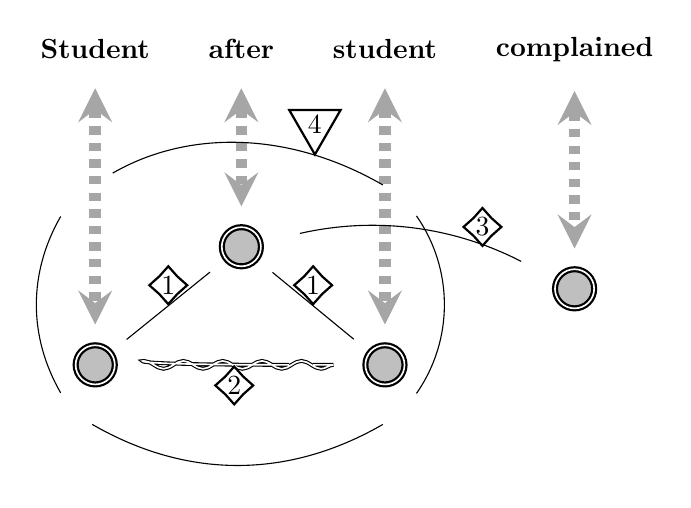
\begin{tikzpicture}

%\tikzset{snake it/.style={decorate, decoration=snake, segment length=5mm, amplitude=15mm}}

%\draw

%\node [s1] at (0,0) {Student};

\node (s1) at (1,1) {\textbf{Student}};
\node (after) [right=5mm of s1] {\textbf{after}};
\node (s2) [right=5mm of after] {\textbf{student}};
\node (complained) [right=5mm of s2] {\textbf{complained}};

\node (s1Rep) [double,draw=black,shape=circle,thick,fill=gray!50,inner sep=.5em,below=3.5cm of s1] {};
\node (afterRep) [double,draw=black,shape=circle,thick,fill=gray!50,inner sep=.5em,below=2cm of after] {};
\node (s2Rep) [double,draw=black,shape=circle,thick,fill=gray!50,inner sep=.5em,below=3.5cm of s2] {};
\node (complainedRep) [double,draw=black,shape=circle,thick,fill=gray!50,inner sep=.5em,below=2.5cm of complained] {};

\draw [ |-,-|, <->, line width = .8mm, draw=gray!70, 
 dashed, double equal sign distance, >= stealth, shorten <= .25cm, shorten >= .25cm ]
 (s1) to (s1Rep);

\draw [ |-,-|, <->, line width = .8mm, draw=gray!70, 
 dashed, double equal sign distance, >= stealth, shorten <= .25cm, shorten >= .25cm ]
(after) to (afterRep);
 
\draw [ |-,-|, <->, line width = .8mm, draw=gray!70,  
 dashed, double equal sign distance, >= stealth, shorten <= .25cm, shorten >= .25cm ]
(s2) to (s2Rep);

\draw [ |-,-|, <->, line width = .8mm, draw=gray!70, 
 dashed, double equal sign distance, >= stealth, shorten <= .25cm, shorten >= .25cm ]
(complained) to (complainedRep);
 
\draw [shorten <= .25cm, shorten >= .25cm ] 
(afterRep) to node [draw=black,shape = star,star points=4,thick,inner sep = 0mm, above] {1} (s1Rep);

\draw [shorten <= .25cm, shorten >= .25cm ] 
(afterRep) to node [draw=black,shape = star,star points=4,thick,inner sep = 0mm,above] {1} (s2Rep);

\node (s1E) [left=-2mm of s1Rep.east]{};
\node (s2E) [left=1mm of s2Rep.west]{};

\draw [shorten <= 2cm, shorten >= .3cm, double, % bend left = 5, 
decorate, decoration={snake, segment length=5mm, amplitude=.5mm}] %, amplitude=15mm]  
(s1E) to node [draw=black,shape = star,star points=4,thick,inner sep = 0mm, below] {2} (s2E);

\draw [shorten <= .5cm, shorten >= .5cm ] 
(afterRep) edge [bend left=20,looseness=1] node [draw=black,shape = star,star points=4,thick,inner sep = 0mm, 
 above, near end ] {3} (complainedRep);

\node (frameTopLeft) [below left = 1.5cm and -.65 cm of s1] {};
\node (frameBottomLeft) [below = 2.5cm of frameTopLeft] {};
\node (frameBottomRight) [right = 3.95cm of frameBottomLeft] {};
\node (frameTopRight) [above = 2.5cm of frameBottomRight] {};

\draw [shorten <= 0.15cm, shorten >= 0.15cm ] 
(frameTopLeft) edge [bend right=30,looseness=1] (frameBottomLeft);

\draw [shorten <= 0.15cm, shorten >= 0.15cm ] 
(frameBottomLeft) edge [bend right=30,looseness=1] (frameBottomRight);

\draw [shorten <= 0.15cm, shorten >= 0.15cm ] 
(frameBottomRight) edge [bend right=35,looseness=1] (frameTopRight);

\draw [shorten <= 0.15cm, shorten >= 0.45cm ] 
(frameTopRight) edge [bend right=30,looseness=1]
node [draw=black,shape = regular polygon,regular polygon sides=3,thick,inner sep = .2mm, 
above, near start, shape border rotate = 180] {4} (frameTopLeft);

%node [draw=black,shape = star,star points=4,thick,inner sep = 0mm, above, 
%bend left=100,looseness=3] {3}

%;


\end{tikzpicture}
\end{minipage}

\hspace{0.1\textwidth}
\begin{minipage}{0.8\textwidth}
			\renewcommand{\labelitemi}{$\blacklozenge$}
	
\begin{itemize}\setlength\itemsep{-.3em}
\item 1 \hspace{12pt}  Head/dependent relation
\item 2 \hspace{12pt}  Argument repetition ({}\BlankAfterBlank{} idiom)
\item 3 \hspace{12pt}  Propositional completion ({}\VisNtoS{})	
			\renewcommand{\labelitemi}{$\blacktriangledown$}
\item 4 \hspace{12pt}  Phrase (modeled as applicative structure), typed as {}\NPl{} 
\end{itemize}
\end{minipage}
\end{figure}
As this shows, the \q{Student after Student} idiom can be notated as, say,
\AfterNSingAndNSingToNPl{} (using \NSing{} and \NPl{} to mean singular
and count-plural nouns, respectively), but with the special case that the \q{argument} to
\i{after} is repeated in both positions, suggesting an unusual degree of repetition,
something frustratingly recurrent: \i{He went on and on}; \i{Car after car passed
us by}; \i{Time after time I got turned down}.
Although I have no problem
treating these constructions as idiomatic plurals, I also contend (on the
premise of phrase-overlap) that the dependent constituents in the \BlankAfterBlank{}
construction can be hooked to other phrases as well (which is why
\q{and [their/his/her] parents} can also be singular, in this case).  I dwell on
this example because it shows how type/functional accounts of phrase structure
can be useful even if we treat phrases more as frames which overlay linguistic
structure, not as rigid compositional isolates.  Each \q{students} variation uses
morphology to nudge cognitive attention in one direction or another, toward events or the
degree to which events are representative of some global property (here of
a student body), or both.  The \NSingToNPl{} transformation is not \i{the}
morphosyntactic meaning, but instead the skeleton on which the full meaning
(via cognitive schema) is designed, its hints solicited.
}
\p{If this analysis has merit, it suggests that a \CAG{}
approach to phrases like \i{many students} or \i{student after student}
(singular-to-plural or plural-to-plural mappings) should be understood not just
as functions among Part of Speech (\POS{}) types but as adding cognitive shading, foregrounding
or backgrounding cognitive elements like events or typicality in some context.
In other words, \i{many students} is type-theoretically \NtoN{} or \NpltoNpl{};
but, in more detail, it adds a kind of cognitive rider attached to the mapping which focuses
cognition in the subsequent discourse onto events (their recurrence and temporal distribution);
similarly \q{student after student} has a \q{rider} suggesting more of a temporal
unfolding.  The second form implies not only that many students complained, but that
the events of these complainings were spread out over some stretch of time.
Each such functional application (mappings between \POS{} understood as linguistic types)
produces not only a resulting \POS{} \q{type}, but also a reconfiguration of cognitive
attitudes toward the relevant situation and context.
Language users have many ways to craft a sentence with similar meanings, and arguably one
task for linguistic analysis is to model the space of choices which are available in a
given situation and represent what specific ideas and effects are invoked by one
choice over others.  It would be an argument in favor of Dependency Grammar if
Dependency-oriented representational models, like Link Grammar, prove to be
especially adept in this modeling.
}
\p{In this analysis, I am already switching to functional and type notions that will be
discussed in greater detail below; my current emphasis is on link grammar as a syntactic
conception, although I have also tried to argue that separating syntax from semantics
can be at most provisional.  Inter-word \q{link pairs} are vehicles for expressing
syntactic rules (like singular/plural agreement) but are also a ground level for
semantic analysis, since we can explain how semantic nuances are carried, in
specific sentences, by the actual link-pairs in evidence (violations to
agreement norms, for example).  These semantic nuances in turn can be given
cognitive interpretations, revealing the syntax-semantics-cognition pattern
which I am sketching here through specific perspectives like Link Grammar and
Type Theory.  Returning to the initial grammatic stage of analysis, however,
my tactics for contrasting overall Dependency and Phrase-Structure paradigms
rest on an implicit picture of how theories should be evaluated.
While such a picture is probably fairly consistent across perspectives, it is still worth
making a little more explicit.
}
\subsection{Explanation and Formality}
\p{Both Dependency and Phrase Structure grammars
presuppose that the fundamental exposition and achievement of their theory involves
formal transformation of linguistic givens, resulting in a more complex data structure
which, to the extent that the theory is correct and useful, models something
of the inner structure of language (\i{qua} abstract formal system and/or cognitive phenomenon).
The \q{data structure} might be a phrase-structure \q{tree} or a graph-like dependency
\q{linkage}, but while these representations have different form they share certain
criteria: they are formally describable systems which allow some structures but reject others;
they are rigorous enough to be given a mathematical (e.g., algebraic) definition;
and they can be expressed in computer code which builds these structures out of
Natural Language artifacts, can verify that an instance of the relevant data structures
satisfies the system rules, and can execute operations which modify the structures.
The phrase trees or word-link graphs are \q{formal substrata} which encapsulate Natural Language
patterns but also are rigidly mathematical and computational.  How thoroughly these substrata
capture linguistic meaning, is therefore directly relevant to questions of whether and
in what degree natural language itself, as social and cognitive, is also formal and computational.
}
\p{Translating NL content into (say) a linked-grammar graph does not make software capable
of \q{understanding} language.  If Dependency Grammar is a reasonable foundation
for linguistics in general, then properly parsing sentences into their
auxiliary graphs is, at most, a step in the direction toward \q{understanding}.
Even this may beg the question of what constitutes a \q{correct} parse: when writing
real-world code, language engineers appear to rely principally on their own intuitions, based
on their familiarity with the underlying theory, the idea they have of what a
\i{correct} \q{re-presentation} looks like (for link grammar, of the correct collection of
link types between the various words).  They then add code to ensure that this representation
is indeed identified by the software in specific examples, and try to do so in such a way
as to generalize to other examples.  This methodology can be gleaned from observing internet chat
sites and other informal research venues; one can witness developers painstakingly constructing
systems which \q{work right} in the sense of producing the interpretation for each sentence
which corresponds with what the human linguists perceive, even for sentences which the
software has never encountered before.  The code is considered reliable the more that
new sentences are \q{correctly} parsed.  Again, \q{correctly} here means, conformant to
linguists' own interpretations; insofar as these are subjective, such conformance is not
conclusive evidence that the transformational algorithms are \q{correct}.
}
\p{In order to assess linguistic \q{competence} (or whatever computational ability may simulate it),
it is needed to check specific \q{behavior} and compare it to some expectation.  The gold standard
for linguistic behavior is just participating in a linguistic community, judged by the community
at large as fully competent and included.  Unfortunately, however \mdash{} at least for those who
want to profit from Artificial Intelligence \mdash{} achieving true \q{language-like behavior} may be
impossible.  Scholarship therefore has to turn toward more limited notions of
competence, such as representational transformation of sentences \mdash{} but since
each theory has its own picture of what sentences should be transformed \i{into},
the justification of competence measures can be circular.  It is the theory which
dictates how the software should act, and the software is deemed \q{intelligent} if it
acts accordingly.  We can be skeptical of such non-theory-neutral conceptions of
\q{intelligence}.  Nonetheless it does count
in theories' favor if they both propose accounts of language structure which
are independently defensible and also can produce computing systems that
reliably and without external direction map language onto those structures.
Language-like behavior then involves producing a transformed representation of
language embodying a particular theoretical conception of
linguistic \q{deep structure}.
}
\p{It would serve Computational-Linguistic theories still further to create systems
that demonstrate behavior which is \q{language-like} on terms less wedded to their
own hypotheses.  More satisfying definitions of linguistic behavior would involve intuitions
of language users in general, not just language experts.  For example, document classifiers
\mdash{} which typically use statistical analysis to predict which topic will be deemed most
relevant for documents like news stories and technical articles \mdash{} again illustate a kind
of transformational representation, converting Natural Language to a formal data structure
(in this case a relatively simple one, naming one or multiple topics from a predefined list).
In this case however a broad user public can provide feedback on how well the system performs.
For another example, artificial translators map language onto formal structures but then
attempt an opposite map, translating the formalized representation into natural-seeming
expressions in a different language.  This case is different in that formal representation is
an intermediary rather than end point of the transformation, but like document classifiers it
is a kind of behavior whose effectiveness can be judged by a large community of speakers.
People who interact with text \q{chat} bots, or talking robots, and feel that the experience
is similar to talking with another person, are also providing evidence of more complete and
larger-scale language-like behavior.  Again, though, it is not now and may never be possible
to engineer intelligent behavior to this level of perfection.  Existing language \AI{} platforms
are flawed but useful, which suggests both that formal re-presentation is an important
step toward language understanding but also that attempts to use these formalisms as a springboard
to more holistic behavior \mdash{} like automated translation, but also extracting practical
information, or gleaning emotion and sentiment \mdash{} are missing something essential.
Doing useful things with or gleaning useful insight from the re-presentational target structures
appears to be a separate problem from that of generating them \mdash{} which calls into question the
degree to which the target structures sufficiently encapsulate linguistic meaning,
even if they reveal structures which are essential to linguistic meaning.
}
\p{This does not have to mean that Natural Language Processing is basically impossible, only
that more modest criteria of \q{correct} \NLP{} systems need to be adopted.  This is complicated
by the fact that artifical language behavior can be flawed but meaningful: \q{Urine shift one
step forward} is an awkward English sentence but its meaning seems clear enough
(this real example comes from a shopping center in New York's Flushing, Queens Chinatown).
We have an intuition that some expressions are \q{incorrect} but not so completely
off-base that they fail to signify anything at all \mdash{} but in this case we need
criteria for how a linguistic performance can be both incorrect \i{and} nonetheless coherent.
}
\p{These issues influence any theory which approaches linguistic competence from the
viewpoint of formal re-presentations, and therefore effectively all branches of
Computational Linguistics.  The reigning assumption appears to be that transformational
representation which converts language to theory-regulated data structures, for which
in many cases the transformation achieved by mechanical algorithms matches that
intuited as most accurate by human experts, serves as \i{prima facie} evidence of
something like computationally-engineered  \q{intelligent (language) behavior}.
This leaves room for language-like behavior to productively replicate dimensions
of language understanding while also being very incomplete: language-like relative
to experts' opinions on deep linguistic structure, not real-world communication.
Structures like link grammar graphs can be essential formal substrata that linguistic expression
relies on to achieve communication, without being the sole medium of this expression.
}
\p{My arguments so far have used Link Grammar as a representative example
of \q{transformational representation} where a computational system
can be judged to reveal some level of language competence, some
kind of \q{language like behavior}, insofar as it translates natural
language expressions to data structures conformant to Dependency
Grammar (and particularly Link Grammar) theory.
As I also just argued, performance \visavis{} structural transformation
may be only tangential to human language, so whatever theory is
built up needs a separate, more philosophical or metatheoretical analysis
to consider how the theory is purported to engage with its phenomena.
But I now take this as a starting point for pivoting the discussion from
grammar to semantics; and will defer until after that speculating
on philosophical implications of the theory thus extended.
}

\subsection{Three tiers of linguistic type theory}
\p{By three \q{tiers} of linguistic organization, I am thinking of
different levels of granularity, distinguished by relative scales of
resolution, amongst the semantic implications of
putative type representations for linguistic phenomena.
Type-related observations can be grouped (not necessarily
exclusively or exhaustively) into those I will call
\i{functional} \mdash{} relating mostly to Parts of Speech and the functional treatment
of phrases as applicative structures; \i{Ontological} \mdash{} engaged with
existential/experiential qualities like sentient/nonsentient, rigid/nonrigid, and
others I have discussed; and \i{Lexical} \mdash{} related to lexemes and word-senses.
The lexical level can include  \q{microclassification}, or
gathering nouns and verbs by the auxiliary prepositions they allow and
constructions they participate in (such as, different cases), and
especially how through this they compel various spatial and
force-dynamic readings; their morphosyntactic resources for describing states
of affairs; and, within semantics, when we look toward even more fine-grained classifications
of particular word-senses, to reason through contrasts in usage.\footnote{So, conceiving microclasses similar in spirit to Steven Pinker in
Chapter 2 of \cite{Pinker}, though I'm not committing to using the
term only in the way Pinker uses it.  Cf. also \cite{AnneVilnat}, which
combines a microclass theory I find reminiscent of \i{The Stuff of Thought} with
formal strategies like Unification Grammar.
}  Microclasses can point out similarities
in mental \q{pictures} that explain words' similar behaviors, or
study why different senses of one word succeed or fail to be acceptable in particular phrases.
There are \i{stains all over the tablecloth} and \i{paint splattered all over the tablecloth},
but not (or not as readily) \i{dishes all over the tablecloth}.  While \q{stains} is count-plural and
\q{paint} is mass-aggregate, they work in similar phrase-structures because both
imply extended but not rigid spatial presence; whereas \q{dishes} can work for
this schema only by mentally adjusting to that perspective, spatial construal shifting
from visual/perceptual to practical/operational (we might think of dishes \q{all over} the
tablecloth if we have the chore of clearing them).  Such observations support
microclassification of nouns (and verbs, etc.) via Ontological and
spatial/dynamic/configuration criteria.
}
\p{Type-theoretic semantics can also apply Ontological tropes to unpack the overlapping mesh of word-senses,
like \i{material object} or \i{place} or \i{institution}.
This mode of analysis is especially well illustrated when competing senses
collide in the same sentence.  Slightly modifying two examples:\footnote{\cite[p. 40]{ChatzikyriakidisLuo} (former) and
\cite[p. 4]{MeryMootRetore} (latter).
}
\begin{sentenceList}\sentenceItem{} The newspaper you are reading is being sued.
\sentenceItem{} Liverpool, an important harbor, built new docks.
\end{sentenceList}
Both have a mid-sentence shift between senses, which is analyzed
in terms of \q{type coercions}.  The interesting detail of this treatment
is how it correctly predicts that such coercions are not guaranteed to
be accepted \mdash{} \i{the newspaper fired the reporter and fell off
the table}; \i{Liverpool beat Chelesea and built new docks}
(again, slightly modifying the counter-examples).  Type coercions are
\i{possible} but not \i{inevitable}.  Certain senses \q{block} certain coercions
\mdash{} that is, certain sense combinations, or juxtapositions, are disallowed.
These preliminary, motivating analyses carry to more
complex and higher-scale types, like plurals (the plural of a type-coercion
works as a type-coercion of the plural, so to speak).
As it becomes structurally established that type rules at the
simpler levels have correspondents at more complex levels, the use of
type notions \i{per se} (rather than just \q{word senses} or other
classifications) becomes more well-motivated.
}
\p{Clearly, for example,
only certain kinds of agents may have beliefs or desires, so
attributing mental states forces us to conceive of their referents
in those terms (\i{Liverpool wants to sign a talented young striker}).
This \i{can} be analyzed as \q{type coercions}; but the type-theoretic machinery should contribute
more than just obliquely stating linguistic wisdom, such as
maintaining consistent conceptual frames or joining only suitably
related word senses.  The sense of \i{sign} as in \q{employ to play on
a sports team} can only be linked to a sense of Liverpool as the
Football Club; or \i{fire} as in
\q{relieve from duty} is only compatible with newspapers as
institutions.  These dicta can be expressed in multiple ways.
But the propagation of classifications
(like \q{inanimate objects} compared to
\q{mental agents}) through complex type structures lends credence to the
notion that type-theoretic perspectives are more than just an expository tool;
they provide an analytic framework which integrates grammar and semantics, and
various scales of linguistic structuration.
For instance, we are prepared to accept some examples of dual-framing
or frame-switching, like thinking of a newspaper as a physical object and a city government
(but we reject other cases, like \q{Liverpool voted in a new city government and signed a
new striker} \mdash{} purporting to switch from the city to the Football Club).  The rules for
such juxtapositions appear to reveal a system of types with some parallels to
those in formal settings, like computer languages.
}
\p{In short, \q{Ontological} types like \i{institution} or \i{place} serve in some
examples to partition senses of one multi-faceted word.  Here they reveal
similar cognitive dynamics to reframing-examples like \i{to the press}, where
Ontological criteria (like reading something as a place) are triggered by
phrase-scale structure.  But there are also interesting contrasts:
the \i{newspaper} and \i{Liverpool} examples
imply that some words have multiple framings which are well-conventionalized;
newspaper-as-institution feels less idiomatic and metaphorical than
press-as-place.  So these examples suggest two \q{axes} of variation.
First, whether the proper Ontological framing follows from other word-choices
(like \q{fire} in \i{the newspaper fired the reporter}, which has
its own semantic needs), or from morphosyntax
(like the locative in \i{to the press}); and, second, whether triggered framings work
by selecting from established word senses or by something more metaphorical.
Metaphors like \i{to the press} do have an element of standardization;
but apparently not so much so to be distinct senses: note how \i{the press} as metaphorical place
does not work in general: \qmarkdubious{}\i{at the press}, \qmarkdubious{}\i{near the press}
(but \i{at the newspaper}, \i{near the newspaper}
\mdash{} imagine two journalists meeeting outside the paper's offices \mdash{} sound quite reasonable).
}
\p{The \q{type coercion} analysis works for mid-sentence frame-shifts; but other
examples suggest a more gradual conceptual \q{blending}.  For example, the
place/institution dynamic is particularly significant for \i{restaurant}
(whose spatial location is, more so, an intrinsic part of its
identity).  Being a \i{place} implies both location and extension; most places are not single
points but have an inside where particular kinds of things happen.  I am not convinced
that restaurant as place and as institution are separate word senses; perhaps, instead,
conversations can emphasize one aspect or another, non-exclusively.  As I have argued,
we need not incorporate all framing effects via \q{subtypes} (restaurant as either
subtype of hypothetical \q{types of all} places or institutions, respectively).  But
\q{placehood}, the Ontological quality of being a place \mdash{} or analogously being
a social institution \mdash{} identify associations that factor into cognitive frames; types
can then be augmented with criteria of tolerating or requiring one association or another.
So if \q{restaurant} is a type, one of its properties is an institutionality that \i{may}
be associated with its instances.  In conversation,
a restaurant may be talked about as a business or community, foregrounding this
dimension.  Or (like in asking for directions) its spatial dimension may be foregrounded.
The availability of these foregroundings is a feature of a hypothetical restaurant type,
whether or not these phenomena are modeled by subtyping or something more sophisticated.
The \q{newspaper} examples suggest how Ontological considerations
clearly partition distinct senses marked by properties like objecthood or
institutionality (respectively).  For \q{newspaper} the dimensions are less available for
foregrounding from a blended construal, than \q{unblended} by conventional usage; that
is why reframings evince a type \i{coercion} and not a gentler shift of emphasis.
The example of \i{restaurant}, in contrast, shows that competing routes for
cognitive framing need not solidify into competing senses, though they trace
various paths which dialogs may follow.
But both kinds of examples put into evidence an underlying
cognitive-Ontological dynamic which has potential type-oriented models.
}
\p{At the most general level \mdash{} what I called \i{functional} type modeling \mdash{} a type
system recognizes initially only the grammatical backbone of expressions, and
then further type nuances can be seen as shadings and interpretations which add substance
to the syntactic form.  So in type-theoretical analysis at this more grammatic level,
to which I now turn, we can still keep the more fine-grained theory in mind:
the relation of syntax to semantics is like the relation of a spine to its flesh,
which is a somewhat different paradigm than treating syntax as a logical or temporal
stage of processing.  Instead of a step-by-step algorithm where grammatical parsing
is followed by semantic interpretation, the syntax/semantics interface can be seen
as more analogous to stimulus-and-response: observation that a certain grammatic
configuration appears to hold, in the present langauge artifact, triggers a marshaling
of conceptual and cognitive resources so that the syntactic backbone can be filled in.
Perhaps a useful metaphor is grammar as gravitation, or the structure of a gravitational
field, and semantics is like the accretion of matter through the interplay of multiple
gravitational centers and orbits.  For this analogy, imagine typed lambda
reductions like \PropToNYieldsN{} taking the place of gravitational equations;
and sentences' grammatic spine taking the place of curvature pulling mass into a planetary center.
}
\p{Parts of speech have \q{type signatures}
notionally similar to the signatures of function types in programming languages: a verb
needing a direct object, for example, \q{transforms} two nouns (Subject and Object)
to a proposition, which I have been notatating with something like \NNtoS{}.
At the most basic level, the relation of Parts of Speech to \q{type signatures}
seems little more than notational variants of conventional linguistic
wisdom like a sentence requiring a noun and a verb (\SeqNPplVP{}).
Even at this level, however, type-theoretic intuitions
offer techniques for making sense of more complex, layered sentences,
where integrating link and phrase structures can be complex.
Even the most broadly scoped analysis of type signatures, dealing only with
generic Parts of Speech like nouns and verbs, can lead to surprising
complications.  One example I have alluded to several times, and will return to shortly:
the problem of applying Dependency Grammar where phrases do not seem
to have an obviously \q{most significant} word for linkage with other phrases.
}
\p{A tendency in both dependency and phrase-oriented perspectives is to define
structures around the most \q{semantically significant} words \mdash{} so that a phrase
like \q{many students} becomes in some sense collapsible to its semantic
core, \q{students}.  Some of my earlier examples, however, argued that
phrases cannot just be studied as replacements for semantic units.  Incorporating
type theory, we can instead model phrases through the perspective of
type signatures: given Part of Speech annotations for phrasal units and then for
some of their parts, the signatures of other parts, like verbs or adjectives
linked to nouns, or adverbs linked to verbs, tend to follow automatically.
A successful analysis yields a formal tree, where if (in an act of semantic
abstraction) words are replaced by their types, the \q{root} type is something like
\Prop{} and the rest of a tree is formally a reducible structure in
Typed Lambda Calculus: \NNtoProp{} \q{collapses} to \Prop{}, \ProptoN{} collapses
to \N{}, and so forth, with the tree \q{folding inward} like a
fan until only the root remains \mdash{} though a more subtle analysis would
replace the single \Prop{} type with variants that recognize different
forms of speech acts, like questions and commands.  In Figure ~\ref{fig:Iknow},
this can be seen via the type annotations: from right to left \NtoN{} yields the
\N{} as second argument for \i{is}, which in turn yields a \Prop{} that is mapped
(by \i{that}) to \N{}, finally becoming the second argument to \i{know}.  This calculation
only considers the most coarse-grained classification (noun, verb, proposition) \mdash{} as I
have emphasized, a purely formal reduction can introduce finer-grained grammatical or
lexico-semantic classes (like \i{at} needing an \q{argument} which is somehow an expression
of place \mdash{} or time, as in \i{at noon}).  Just as useful, however, may be analyses
which leave the formal type scaffolding at a very basic level and introduce
finer type or type-instance qualifications at a separate stage.
}
\p{In either case, Parts of Speech are modeled as (somehow analogous to) functions, but the important
analogy is that they have \i{type signatures} which formally resemble functions'.
Phrases are modeled via a \q{function-like} Part of Speech along with one or more
additional words whose own types match its signature; the type calculations
\q{collapsing} these phrases can mimic semantic simplifications
like \q{many students} to \q{students}, but here the theory is explicit
that the simplification is grammatic and not semantic: the collapse
is acknowledged at the level of \i{types}, not \i{meanings}.  In addition,
tree structures can be modeled purely in terms of inter-word relations
(this is an example of embedding lambda calculii in process algebras),
so a type-summary of a sentence's phrase structure can be notated and
analyzed without leaving the Link Grammar paradigm.
}
\p{As a concrete example, in the case of \q{many students},
both \q{students} and the semantic role of
the phrase are nouns (count-plural nouns, for where that's relevant).  Accordingly,
\q{many} has a signature \NtoN{} (or \NpltoNpl{}, dependending on how
narrowly we want to notate the types in context).
Once we assign types and signatures to all words in a sentence, we can also see a
natural hierarchy resembling an expression in typed lambda calculus, where some words
appear as \q{functions} and others as \q{arguments}.  Often the less
semantically significant words appear as \q{higher} in the structure,
because they serve to modify and lend detail to more significant words.
The kind of structure or \q{Charpente} which falls out of a sentence \mdash{}
adopting a term from \Tesniere{} (cf. \cite[p. 181]{ElkeTeich}) \mdash{} is typically different from a link-grammar
\q{linkage}, although the two structures can be usefully combined.
}
\p{To return to the example of \q{Student after student}, where designating
one word to \q{represent} the phrase seemed arbitrary, we can analyze the
situation via type-signatures.  I have teased a proposed solution repeatedly;
here's what I had in mind.  Insofar as \i{after} is the only non-noun,
the natural conclusion is that \q{after} should be typed \NNtoN{}
(which implies that \q{after} is analogous to the \q{functional} position, and
in a lambda-calculus style reconstruction would be considered the \q{head}
\mdash{} Figure ~\ref{fig:ESA} is an example of how
the sentence could be annotated, for sake of discussion).
This particular idiom depends however
on the two constituent nouns being the same word (a pattern I've also alluded to with
idioms like \i{time after time}), which can be accommodated by invoking the (computationally rather complex
and topical) concept of \i{dependent types} \cite{BernardyEtAl}, \cite{TanakaEtAl}
\mdash{} in other words the parameters
for \i{after} are a dependent type pair satisfied by an identity comparison between
the two nouns.  The signature for \q{after} has this added complication, but
the nuances of this example can still be accommodated within the overall
architecture of type theory.  I would pair this argument with my earlier
analysis of \q{many} variations which suggested how apparent complications
can be accommodated largely within the extant theoretical resources of
Link Grammar, and in combination suggest that the union of Link Grammar
with Type-Theoretic Semantics seems poised to accommodate many
complex real-world linguistic cases with a coherent abstract perspective.
}
\p{Consider alternatives for \q{many students}.  The phrase as
written suggests a type signature (with \q{many} as the \q{function-like} or
derivative type) \NpltoNpl{}, yielding a syntactic interpretation of the phrase; this
interpretation also suggests a semantic progression, an accretion of intended detail.
From \i{students} to \i{many students} is a conversion between two plural nouns
(at the level of concepts and semantic roles); but it also implies relative size,
so it implies some \i{other} plural, some still larger group of students from which
\q{many} are selected.  While rather abstract and formal, the \NpltoNpl{} representation
points toward a more cognitive grounding which considers this \q{function} as a form
of thought-operation; a refinement of a situational model, descriptive resolution,
and so forth.  If we are prepared to accept a cognitive underpinning to semantic
classification, we can make the intuition of part of speech signatures as \q{functions}
more concrete: in response to what \q{many} (for example) is a function \i{of},
we can say a function of propositional attitude, cognitive schema, or attentional
focus.  The schema which usefully captures the sense and picture of \q{students} is
distinct (but arguably a variation on) that for \q{many students}, and there is a
\q{mental operation} triggered by the \q{many students} construction which
\q{maps} the first to the second.  Similarly, \q{student after student} triggers a
\q{scheme evolution} which involves a more explicit temporal unfolding
(in contrast to how \q{many students} instead involves a more explicit
quantitative \i{many/all} relation).  What these examples show is that
associating parts of speech with type signatures is not just a formal
fiat, which \q{works} representationally but does not necessarily capture
deeper patterns of meaning.  Instead, I would argue, type signatures
and their resonance into linkage acceptability structures
(like singular/plural and mass/count agreement) \i{point toward} the
effects of cognitive schema on what we consider meaningful.
}
\p{In \i{Student after student came out against the proposal},
to \i{come out}, for/against, lies in the semantic frame of attitude and expression
(it requires a mental agent, for example), but its reception
carries a trace of spatial form: to come out \i{to} a public place, to
go on record with an opinion (a similar dynamic applies to the idiomatic
\q{come out} to mean, for someone gay or lesbian, \q{come out of the closet}
\mdash{} in that idiom the spatial figure is explicit but metaphorical).  Usually
\q{come out [for/against]}, in the context of a policy or idea, is similarly
metaphorical.  But the concrete spatial interpretation remains latent, as a kind
of residue on even this abstract rendition, and there sustains a chance that this
undercurrent will actually figure in conversants' mutual understanding \mdash{} if
there were not just columns being written and opinions voiced but demonstrations
on the quad.  The spatial undercurrent is poised to emerge
as more literal, should the context warrant.  However literally or metaphorically
the \q{space} of the cognitive \q{coming out} is
understood, however explicit or latent its cogitative figuration,
is not something internal to the language; it is a potentiality which
will present in different ways in different circumstances.  This is not to say that
it is something apart from linguistic meaning, but it shows how linguistic meaning
lies neither in abstract structure alone, nor contextual pragmatics, but in their cross-reference.
}
\subsection{Levels of formalization}
\p{Of the three type levels I have proposed, the \q{functional} level is the most
quasi-mathematical; for other levels, formal type theory may provide interpretive
tools and methodological guides, but formally representable framings and
transformations may be only approximations of how people actually think, while
they are understanding language.  From this perspective, we are left with the
metatheoretical question of clarifying how different kinds of analyses, which
put different degrees of weight on formal or on interpretive argumentational,
are to be joined in overarching theories.  In particular, are the
linguistic phenomena which seem to demand more \q{interpretive} treatment actually
beyond formalization, or is it just impractical (but possible in theory) to provide
formal analysis of each individual case-study, each real-world language formation?
Is Natural Language actually no less formal than (for example) computer programming
languages, except that the former have a much larger set of semantic and syntactic
rules such that any analysis can uncover them only partially?  Or is any rule-based
model of language, no matter how complete, necessarily partial relative to real language?
}
\p{Computer languages are a good case-study in what I might call \q{semiotic computability}.
This designates the question of whether the
operations of sign-systems \mdash{} how sign-users express intentions by forming or modifying
structured networks of signs that explicitly exhibit or are understood to have been
formed according to collectively recognized signifying rules \mdash{} can be modeled,
at least to some substantial degree, by computable algorithms.  Our
notion of computation can be based on modern computer code, not just academic
topics like pure functions: the behavior of computing systems
where many functions run concurrently, with possible side-effects, is often
non-computable via static analysis; such systems can only be understood by
actually running them.  Nevertheless the capabilities of software programmed
in modern languages certainly deserve to be characterized as \q{computable}
behaviors.  A single function, which embodies a computable
calculation, may be part of a process space whose evolution through
time is nondeterministic, and computing environments which employ
functional side-effects are difficult or impossible to evaluate in the abstract.
I use \q{computability} therefore in this wider sense: operationally implementable
according to theories underlying mainstream programming languages, which is
conceptually (if perhaps not mathematically) distinct from \q{computability} in
subjects like algorithm analysis.
}
\p{Natural Langauge Processing, working with human languages from a computing platform,
is then a step further, continuing beyond logico-mathematic abstractions and toward
empirical language-use.  We can consider at what point formal and computational methods reach a limit,
beyond which they fail to capture
the richess and expressiveness of Natural Language, or whether this limit itself
is an illusion \mdash{} whether even fully human
language competence is (perhaps in principle if not in practice) no less reducible
to formalizable patterns.  Using the wording I just proposed, we can speculate on
whether all language is \q{semiotically computable} or whether language merely
depends on faculties which in some neurological and/or presentational sense are
\q{computable} in those terms \mdash{} faculties that, measured against linguistic fluency,
are necessary but not sufficient.
Whatever one's beliefs on this last question,
a progression of subdisciplines \mdash{} from formal-logical semantics through programming
langauges and computational Natural Langauge Processing \mdash{} is a reasonable
scaffolding for a universe of formal methods that can build up, by progressive theoretical
sophistication or assembly of distinct analyses which piece together jigsaw-like, to model
real-world language understanding.  Perhaps real language is an \q{emergent property} of
many distinct algorithms that run and combine in the mind; or perhaps the relevant
algorithms are a precondition, presenting cognition with essential signifying givens
but fleshed out in other, more holistic ways, as we become conscious of language not
just as a formal system but an interactive social reality.
}
\p{I have sketched a similar theoretical progression, starting with a theory of
grammar (Link Grammar), transitioning to a form of semantics (a type-theoretic semantics
defining type hierarchies and signatures over linkage graphs), and finally proposing a
cognitive interpretation of the resulting semantics.  I will refer to this
\i{interpretation} as  \q{Cognitive State Semantics}, meaning that such a theory
adopts its \i{formal} structures from Link Grammar and type-theory but also attempts
to \i{motivate} these structures by appeal to cognitive considerations.  Both Link Grammar
(through its specific Category of labeled graphs modeling sentence linkage-structures) and
Type-Theoretic Semantics work with rigorous, algebraically formal models satisfying criteria
I referenced at the end of the last section: translation of language content into these
formats and subsequent review or transformation of the target structures can be programmed
as a purely mechnical space of operations.
}
\p{By itself, the superposition of
type-theoretic semantics on link-grammar graphs does not cross a hypothetical \q{barrier} between
the formal and the cognitive.  But I intend here to suggest a cognitive \i{interpretation}
for the formal structures; that they represent an outline of cognitive schema, or progressions,
or represent linguistic \q{triggers} that a cognitive language ability (taking language
as part of an environing world and produced by others, in rule-bound social situations,
to communicate ideas and sentiments) responds to.  This range of interpretations is
deliberately open-ended: we can say that a formal infrastructure grounds the cognitive
reception of language givens, without arguing specifically that formal structures identified
in language therefore model cognitive operations directly, or that these are instead
patterns identified in language that trigger a cognitive response, or any other
paradigm for mapping cognition as process and activity to language structure as model and
prototype.  Leaving these options open, however, I will focus in the remainder of this
paper on one interpretation, considering formal structures as \q{triggers} which
get absorbed into language understanding via observatory propensities: as language
users (on this proposal) we are disposed to identify certain formal structurations
operating in language as we encounter it, and respond to these observations by building
or refining mental models of the situations and signifying intentions we believe have been
implied by the discourse, in evolving and intersubjective dialogic settings that involve
joint practical activity as well as communication.
}
\p{In this sense, I believe natural language reveals mutually-modifying juxtapositions
of concepts whose full semantic effects
are probably non-computable: I would work on the assumption that language
\i{as a whole} and as human social phenomena is not \q{computable} in a
semiotic sense, or any related practical sense (although
I make no metaphysical claims about the \q{abstract} computability of mental
processes merely by virtue of their neurophysical materiality).
The aforementioned \q{linguistic side effects} can be \i{modeled} by tracing our reception
of linguistic meaning through syntactic and semantic formations, like Link Grammar
and Type Theory, but I argue for such models not as models \i{of} cognitive processes,
but rather models of \i{observations} which trigger cognitive follow-up.  Even if we
believe in and practice a rigorous formalization of morphosyntactic structure,
where the \i{pattern} of conceptual \q{side-effects} can be seen as
unfolding in algorithmic ways, the cognitive \i{details} of these
effects are too situational, and phenomenologically rich, for
computability as ordinarily understood.  But the formal structure is
not wholly irrelevant: to call up nuanced cognitive schema
\mdash{} or so I submit for consideration \mdash{} may not be possible without
algorithmically reproducible lexicosemantic and morphosyntactic triggers,
at least modulo some approximation.  A (perhaps non-computable) space
of cognitive schema may be projected onto a (perhaps computable)
set of affiliated morphological patterns, using notations like
link-grammar pairs and type signatures to catalog them.  For example, there may be a non-computable
expanse of possible construals of pluralization; but any such construal,
in context, is called into focus in conversants' minds by morphosyntactic
invitations, by speakers' choices of, say, \mbox{\NSingToNPl{}}-pattern
phrases.  The important balance is to take formalization as far as is reasonable
without being seduced into logico-symbolic reductionism \mdash{} a
methodological pas de deux I will explore further in the next, concluding section.
}
\p{Any word or usage invites various facets to either
emphasize or deemphasize, and these subsumed concepts or foci are
latent in potential meanings, brought into linguistic space
by the play of differentiation \footnote{Alluding, in part, to Sausurrean \q{system of differences}
\cite[p. 15]{EfePeker} \mdash{} to choose a reference which introduces
Sausurre in a rather unexpected context.
}
: \i{baked}, not \i{made}; \i{flew}, not \i{traveled};
\i{spill}, not \i{pour}.
These under-currents of subsidiary concepts and foci are selectively hooked onto by
morphosyntactic selection, so in analyzing phrase
structure we also have to consider how using syntax
which constructs a given structure also brings to the forefront certain
nested concepts and construals, which are latent in word-sense options;
in the topos of lexicosemantic possibilia.
}
\p{So, any talk about \q{side effects} of morphosyntactic functions
\mdash{} mapping verb-space to adjective-space, noun-space to
proposition-space, singularity to plurality, and so forth \mdash{} should consider
a type-theoretic gloss like \NtoN{} as sketching just the motivating
scaffold around an act of cognitive refocusing.  The interesting semantics
lies with \i{how} a sense crosses over, in conversants' minds,
to some other sense or concept, wherein other aspects are foregrounded
\mdash{} for example, within temporal event plurality: multiplicity as
frequency, or episodic distribution relative to some time span;
or suggesting something that is typical
or predominant; or relative count against some other
totality \mdash{} each such refocusing triggered by a phrasal construction
of the form \NtoNpl{} or \mbox{\NpltoNpl{}}.
Or we can map singulars, or count plurals, to mass nouns, and vice-versa (\i{shrubs} become \i{foliage};
\i{water} becomes \i{a glass of water}).
The plural and the singular are a coarse-grained semantic that has not yet arrived as \i{meaning}.
Conceptual spaces guide attention to classes and properties, defining a path of ascending
precision as speakers add descriptive detail;
cognitive construals negotiate relations between different kinds
of aggregates/individuals; individuality, aggregation and multiplicity as phenomena and
disposition.  These construals are practical and embodied, \i{and}
phenomenological \mdash{} they direct attention (\i{qua} transcendental universal of
mentality, if we like), to and fro, but in the course of intersubjective and
goal-driven practical action (and in that sense particular, world-bound, historicized).
}
\p{Given these considerations, I propose a \q{Cognitive State Semantics}
\mdash{} understanding phrase structure in terms of (or analogous to) functional effects
(like \cite{ShanThesis}), but cognitive: word and syntax choice effectually
steering cognitive appraisals of jointly experienced situations
in specific directions.  Cognitive State Semantics also has formal implications:
the inner structuration of data \q{spaces},
including unknown and undefined values, and including (side-effects-bearing) function types,
can be understood as dynamic \i{states of knowledge} and their changes, grounding datatype semantics in human
use/interactions.  Linguistically, the \q{effects} of language \q{functions} are
mutations/modifications in cognitive state, respondant to concrete
or abstract scenarios which are topics of dialog.  Sometimes, effects may
tolerate mathematical analysis; but such analytical thematics tend to peter out into the
ambient, chaotic worldliness of human consciousness.
}

\section{Conclusion}
\p{Without reducing linguistic \i{performance} to language qua
field of propositional expression, and without collapsing linguistic meaning
to a computable/propositional fragment, we can still allow
interpretive-phenomenological and formal/mathematical perspectives to co-exist.
In the theory I have sketched, Cognitive Schema summarize lived, situated
judgments and intentions that (in concrete form) are not \q{computable}
(again with the caveat that our mostly science-driven worldview may imply
that all reality is \q{computable} in some infinitely-powerful computation;
I understand \q{computability} to terminologically exclude
such a purely speculative level of capacity).
However, our propensity to call up certain construals rather than others is triggered by
linguistic formations, and in broad outline the catalog of these triggers,
and their compositional structure, can be formalized (and even
used to improve formal systems, like programming languages).  The
challenge is to advocate for this co-existence without implying
that formal systems, and mathematically provable system-properties,
are the only kind of research tools which have scientific merit.
}
\p{Subjective assessments are intrinsic to most linguists' argumentation \mdash{} warranting
claims not with empirical data or logico-mathematical proof but by appealing to
speakers' intuitions, so that reading linguistic texts is also collaborating
on an ongoing research project (partly because language evolves, so
word-meanings change, and formations which are ungrammatical for one generation
may be experienced differently by others).  Nevertheless, linguistics, like
economics, seems broadly accepted as a human \i{science}, not just an
interpretive discipline.
The claim that an economist's equation or a linguist's meta-grammar
are accurate explanations, useful explanatory frameworks, seems generally
evaluated in terms of whether their framework captures emergent higher-order
structure, and offers an explanatory potential that does not merely reiterate lower-scale
paradigms.  A theory expressed in the language of linguistics (not, say,
neural networks), if it meets general criteria of testability and refutability
(not necessarily empiricist/quantitative),
arguably carries even more weight than lower-level neurophysical
explanation \mdash{} precisely because the higher-scale \q{theory language} carries the burden of
explaining emergent properties, which as \i{emergent} bear some
descriptive/behavioral (if not causal) autonomy.  Likewise, a subjectively plausible
and theoretically motivated equation which fits economic data
probably carries more weight than a mere statistical analysis.  An explanatory focus
on the higher-scale in terms of its own distinct (emergent) structures and theorized
entities (like words and morphemes, in the case of linguistics, or markets and commodities,
in the case of economics), reflects the linguist's or economist's charge to connect
human phenomena with mental (and therefore, ultimately physical) law.  Nonetheless,
even with liberal use of subjective judgments, economics and linguistics (and some
other human sciences as well, potentially) are attached to the overall sphere of
natural science, by virtue of causal links in principle even if not in practice.
Scientific rigor in this humanistic setting is neither reducible to the techniques
of natural science, nor dualistically separate from them.  Natural
science and humanities are certainly not mutually irrelevant, but nor is
the proper vehicle for scientific literacy to find a forum in the humanities
merely to emulate numeric methods, as with statistics in sociology, or
a retreat to narrow and behavioristic reductionism, in
place of localized interpretation and situational particularism.
}
\p{Subjective impressions (conscious experiences, emotions, intuitions, qualia, qualitative universals and
particulars \mdash{} the qualitative characteristic in itself, and the hyletic-spatial trace,
the site in experiential space as the quale becomes a moment of consciousness) \mdash{} these are not scientifically
tractable and do not have obvious physical location or measurability, which makes them controversial as
objects of scientific method.  Yet, even so, we do have conscious experiences, we
do subconsciously (and when needed consciously, or with deliberate conscious attention)
make judgments about classifications, or how parts aggregate into wholes, or are individuated
apart from a larger whole in context; we can reflect on patterns in these judgments,
not \i{introspectively} examining thoughts as they occur, but marshalling an overall
familiarity with mental processes.  Consciousness is not only a kind of mentality,
shared by humans and some animals; it is also a metacognitive tool, something we
deploy to focus attention on a certain object or topic.  We \q{practice} how to \i{be}
conscious, how best to distribute attention, in each setting
(like an athlete maintaining a meditative state of ambient awareness,
poised to latch conscious attention onto playing technique which is optimally instinctive,
but \q{feels} different when degraded by fatigue or distraction).
Our faculty for these modulations, switching among sub- and passive consciousness,
attentive consciousness, \q{ambient} awareness, and back again,
reveals that consciousness is not only an aspect of mind
but a tool; it has a meta-cognitive and epistemic dimension,
an awareness of what is known or not-yet-known and a technique of directing attention to the
latter.
}
\p{A case-study: in a motel I unexpectedly find a newspaper outside the
door.  Next morning I look outside curious whether a paper is there; after several days
I come to expect the paper.  So I open the door not preoccupied with confirming this, but
with (maybe rather distractedly) fetching it.  Initially I do not expect the paper, but, generally poised
to notice both expected and unexpected circumstances, I make a mental adjustment and
interpret the situation quickly; by the third day the paper has become expected,
like other things I anticipate finding in a motel hallway, and the thrust of my attention,
during the brief episode of my picking it up, is kinaesthetic and motor-intentional
more than visual and inquisitive.
Only on the second morning is the question of a paper's presence intended
in an epistemic mode; but, while it is so thematized, I direct attention
to optimize my ability to resolve the question.  How we engage attention is a
deliberate choice, reflecting and responding to our metacognitive attitudes,
what we think we know and do not know.
}
\p{Because consciousness is in some ways a mental tool, we have an intimate familiarity with it, a
familiarity which extends beyond our own minds: we can make reasonable guesses about what
others do or do not know and perceive.  Our ability to anticipate others' epistemic states
is an intrinsic feature of social interaction, of intersubjectivity;
we therefore understand consciousness not only via our
own use and possession/experience of it, but as a general feature of the human mind.
We can accordingly make structured claims about conscious processes, not
in the sense of introspective reports but of retrospective suggestions \mdash{} by analogy, a
pianist on reflection may have alot to say about playing technique, but she does not
acquire this wisdom from introspective study of her own playing while it happens;
rather with accrued wisdom and reflection.  In terms of phenomenological method, our study of thought
and consciousness is analogous: it is reflective examination of what it means to be
consciously intelligent beings, not introspective psychology, or meditative meta-experience.
}
\p{The methodological implications of this retrospection
(as opposed to \i{intro}spection), how phenomenological writing seeks
reflective consensus on claims about consciousness \mdash{}
this fashion of constructing a research community, a discursive-methodological
field, does not conform to empirical scientific method, but is arguably a quite
valid and defensible means of meeting the criteriological goals \mdash{} the discourse
ethics, the democratization of scientific participation \mdash{} which
physical science achieves via empiricist Ontology.
For all its limitations, Positivism
has the one virtue of disputational inclusiveness, demanding potential
observability (not some special revelation or insight)
for theoretic ur-entities.  The civic norms of phenomenology are more complex, because both
\q{transcendental} analysis of consciousness \mdash{} as a kind of philosophical ground zero, a neo-Cartesian
fortress against skepticism and empiricism \mdash{} and also a more pluralistic, enculturated,
embodied, social phenomenology, are well-represented (and interpenetrate in complex ways)
in the continuing post-Husserl tradition.  That being said, even in its most neo-Idealist, reifying consciousness
as a primordial frame on any cognitive-scientific reasoning, as human sciences' condition of
possibility, phenomenology cannot help but textually acknowledge pluralism, and philosophical
collaboration \mdash{} precisely because its claims are not descriptive of empirically locatable/observable objects.
}
\p{Interestingly, the phenomenological tradition reveals substantial interest in both
the socio-political and the formal-mathematical: this is not so noteworthy
in itself, because Analytic philosophy also connects (say) language with
(say) logic, but phenomenology is distinct in that
it joins the humanistic and the formal/mathematical without the same
tendency to hone in on a overlapping, logico-semantic core.  In writings where
Analytic philosophers appear to address both social and mathematical concerns, usually their
underlying motivation, or so it seems to me, is to find some logical
underpinnings to linguistic or cognitive structure (say, \i{implicatures}) \mdash{} logic, subject
to formal treatment, also manifesting itself in the organization of thoughts and
expressions.  Amongst phenomenologists, however, for example Husserl,
Merleau-Ponty (in his science-oriented writings; \cite{DavidMorris}), and Anglo-American
writers in the \q{Naturalizing Phenomenology} tradition,
there is evident interest in mathematics \i{apart from} logic: topology,
differential geometry, mereotopology, multi-granularity.\footnote{Not that logic is wholly unrelated to these subjects: consider
topological and type/Category-theoretic embeddings of logical systems
within certain categories, or technical domains, like toposes, sheaves, granules;
but logic in this sense, mathematically founded within spaces otherwise discussed
at least as metaphoric guides within phenomenology, does not
appear to be the dominant understanding of logic in the Analytic
philosophical tradition.  To be fair, style may dictate that
argumentation should be trimmed to its essential elements, and
mathematical deductions are rarely if ever essential for
defending phenomenological claims.  In Jean Petitot, for example,
mathematics is sometimes intrinsic to empirical backing for
phenomenological ideas, but other times (say, sheaf mereology),
the formal theories, while useful analogies, do not clearly pair up with
logico-deductive justifications.  But, I would reply, there
is so much unexplained about consciousness, and cognition
as it occurs in conscious minds --- the controversial \q{Explanatory Gap}
between mind and matter --- that much of the important
argumentation does not yet have deductive signposts; we need an
effective methodology which is not so linear.
As we approach beyond a simplifying, logico-functionalist vantage,
which we eventually must transcend, both functionalization and empiricism
fall by the wayside as reasonable methods for \q{Naturalizing} consciousness.
We have to accept when the formal/mathematical stands as more intuitive
than rhetorical, on pain of \q{Naturalization} being quarantined
from a humanistic core entirely.
}
Phenomenology therefore uncovers
an arguably deeper and truer bridge between human and \q{eidetic} sciences,
in Petitot's phrase, one which is not pre-loaded with logico-reductive presuppositions.
If this is accurate, phenomenology can provide a deeper methodology
for the humanities in their interactions with natural science.
Even insofar as we stay committed to the idea
that social/cultural/mental phenomena emerge from (neuro-)physical ones, we
need to curate methods for these \q{emergent} sciences which have the requisite
theoretical autonomy to actually extend the explanatory reach of the natural
sciences on which they causally rest.  Cognitive Linguistics, I would argue,
is a good example of this notion of autonomy, and its methodology, I would
also argue, bears an important resemblance to phenomenological research.
}
\p{Another brief case-study (revisiting footnote \ref{footnoteVision}):
our environing world mostly discloses itself through objects' visible exterior:
as much as we have on occasion a palpable sense of volume as well (as when looking through a fog)
\mdash{} and as much as what we see is inextricable from our embodied interactions with objects,
adding tactile and kinaesthetic dimensions, a canonical sense of perception
is still the vision of distant objects, usually through their
surface geometry.  A canonical example of perceptual
cognition is therefore reconstructing geometry from visual appearances,
especially color gradations \mdash{} mathematically, converting \q{color} vector
fields to curvature vector fields (it's worth noting that color is an
almost primordial example of a Conceptual Space Theory as developed
by \Gardenfors{} and others \cite{Strle}).  This kind of transformation,
described (say) via differential geometry, is \i{qua} theoretical device
an example of semiotic morphism, a mapping between
representation disciplines \cite{GoguenSemioticMorphism}, \cite{GoguenWhatIs}.
The point is not, however, that there are precise correlates in the brain which
\q{implement} this procedure; that the semiotic morphism takes
a domain and codomain that quantify over empirically locatable,
neurophysical entities.  We can study how software reconstructs
geometry from color data as an approximation to a \i{process},
a model-building whose semiotics of approximation is coarse-grained and
holisitc.\footnote{The experiential verisimilitude of computer graphics is a
phenomenological data point, but so is their obvious unreality \mdash{}
the mathematics reveals something about, but is not an all-encompassing
model for, shape and color \i{qua} material phenomenon, still less
the neuroscience of color experience.  Morphism between structures
may model \i{processes} more correctly than the structures themselves approximate their substrata
\mdash{} but this is no longer a semiotics of causal/physical reductionism,
a use of mathematics (like differential geometry) to iconify empirical givens, the way
that (say) the Navier-Stokes equations are understood to refer explicitly to (even while idealizing
and abstracting from) fluid-mechanical dynamics.
Our theory-semiotics has to locate the site of designation
at a more oblique scale, a different Ontological register, of processes and
transformations \mdash{} seeing in phenomena the image of a theoretical
model because of its global structure, as a sign in its own right,
rather than a collage of symbols and numbers to which are
reduced spatializations and trajectories of causation and physical influence.
}  Formal
devices like vectors or vector fields need not mold symbolic systems
by mapping individual symbols to spacetime objects, or processes, but rather
afford representation-mappings that capture cognition indirectly and patternwise.
}
\p{I make this point using visual consciousness as an example, but it applies
also to cognitive grammar, where the color -to- curvature-vector
morphism has an analogue in the mapping of word-sequences to tree- or graph-algebras.
I do not intend to claim that there are specific, individuated neurophysical
analogues to theoretical posits in the symbolic regime I sketched earlier,
in terms of \POS{} and lexical annotations, inter-word and inter-phrase connections,
applicative structures, and the rest.  There are not, necessarily, for example,
little brain regions whose role is to represent different types of
phrase structures (e.g., different flavors of pluralization).
Our explanatory ambitions, instead, should be cognitive-linguistic models of a
global process-structure, agnostic about one-to-one correspondence between the posits of the theory and the
empirical stuff whose behaviors it wants to explain.  Cognitive triggers bridge formal/empirical sciences with
the phenomenological/humanistic: their causal engenderings are physical and structural phenomena, but their
manifestation in the world is not fully tractable without an interpersonal deliberation accounting for both the
privateness of consciousness and the sociality of mind, and, so, something akin to phenomenology.
}
\p{It may appear that I am describing a weak-functional theory (or metatheory)
which uses functional description in lieu of precise micro-physical
explanation \mdash{} in other words, that in lieu of explaining precisely how
the brain achieves vision or language, we describe functional capabilities
that are prerequisite for these competences, and refactor the goal
of scientific explanation as to describe the system of intermediate functionality
as correctly as possible, rather than describe how this functionality
is physically realized.  In a strong form, this re-orientation yields
functionalism in theories/philosophies of Mind, that try to refrain from
Ontological commitments to mental states or properties \i{apart from} descriptions of
their functional roles.  In other words, according to the
parameters of the field of study and its institutions, even if not deep
metaphysical beliefs, mental states are reducible to functional states, and cognitive
systems are scientifically equivalent if they reveal similar functional organization, whether
they belong to human or animal minds or computers or extra-terrestrials.  A
more modest functionalism would reject the implied reductionistic
(maybe eliminative) Ontological
stance, and maintain that mental things are not wholly, metaphysically subsumed
by their functional organization, while still practicing a kind of
theory whereby this functional organization is the proper object of
study; the specific aspect of the mental realm
which is scientifically tractable.
}
\p{I do not believe I am making even such weak-functionalist claims:
either branch of functionalism can misattribute the methodological
association between theoretical structures and explanatory goals.
We may be led toward the stronger or weaker functionalist viewpoints
if we understand that a cognitive theory should task itself with making
symbolic icons for scientifically grounded referents, grounded in an abstract
space of functional organization if not in empirical space-time.
Of course, most scientific explanation does construct a specialized,
technical semiotics whose signs refer into either formal spaces or
accounts of empirical space-bound things, however abstracted or idealized.
But, conversely, insofar as I propose to focus on functional structures, and particularly
cross-representation-framework transformations, my intent is to
\q{functionalize} the discursive norms of the theory, not the
phenomena it investigates.  In order to negotiate between the competing
demands of scientific rigor and formalization \mdash{} on the one hand \mdash{}
with the immediacy and etheriality and subjectivity of consciousness, on the other,
we need to \q{attach} theoretical structures to mental phenomena without
getting bogged down in questions of the scientific or Ontological
status of mental things, how they are \q{scientific} individually and collectively
(collectively as in the Ontology of \q{Mind} overall).
}
\p{This suggests adopting functional attitudes not
in the theory but the metatheory: to use functionalism as an organizing
principle on the theoretical \i{discourse}, on the attitudes of the
scientists and scholars who want to straddle the divide between natural
and mathematical sciences and humanism and consciousness.  The
\q{semiotic morphism} of color-to-curvature vector fields, or word-sequences
to typed semantic graphs, are recommendations for guidelines on how
researchers should write and communicate about cognitive processes in their
global structure.  I have tried to outline a metadiscourse more than
a metalanguage \mdash{} not a template for building theory-languages whose
signs refer into a realm of posited empirical or abstract entities, but a
template for using certain formal-mathematical constructions (in
domains like typed lambda calculus, type theory, or differential geometry) as a
textual prelude, a way to position the norms of writing to be receptive
to both scientific-mathematical and phenomenological concerns.  If
semiotic morphisms like color-to-curvature or word-sequence-to-semantic-graph
have explanatory merit as ways to picture cognitive processes, this
merit is intended to be judged according to how it affects
discursive norms on this scientific borderlands between mathematics
and humanities, rather than how it reduces empirical phenomena
to mathematizable abstractions.  If there is \i{something} in cognition
analogous to these morphisms, even if \q{analogous} means merely that
holding the morphisms as formally defined in our minds while
thinking about cognition can show us philosophical ways forward,
then we should be interested in refining these
formalizations as part of the overall Cognitive-Phenomenological project.
}
\decoline{}
\p{The Cognitive-phenomenological project is very different, I believe,
than the AI or Atificial General Intelligence
projects.  Nevertheless, as I noted to conclude
Section 5, AI \mdash{} for all its reductive ideology \mdash{}
does show the benefits of an intellectual framework
where researchers can experiment, try things out, and
write code.  We should not underestimate the power
of technology and experimentation to ground and engage
the scholarly process: it allows the scholar to
program her own research environment, autonomous
as necessary from academic and institutional paradigms
\mdash{} which, notwithstanding a general acaemic
commitment to innovation, can get
mired in inertia: particularly when it
comes to interdisciplinary methodology
and particularly when it comes
to reengineering the publishing
process and the dissemination of scholarship.
There is a lot of technical and technological
potential which in the acaemic and publishing
communities is not being realized.
}
\p{This is not just a procedural claim
tangential to actual scholarly argumentation:
we need new generations of publishing
tools to properly syntheize computational
technology with nonreductive,
humanities-based philosophies of mind
and consciousness.  We need to properly
implement the technological tools
that empowe individual scholars,
without buying uncritically
into academic and corporate appropriations
of technology for regressive ends.
}
\p{At the risk of
seming to conclude with an infomercial, I'll
cite as an example the Conceptual Space Type Theory
and Type Expression Language (CSTX), which is
currently used in the context of scientific data publication
(see my forthcoming chapter in \cite{NathanielChristenCyberphysical}).
CSTX presents a flexible type theory that can model
both natural-langauge phenomena (such as
Link Grammar, the internal parsing formalism in
OpenCog, and the type-theoretic semantics favored by
linguists such as Zhaohuu Luo or
James Pustejovsky) as well as formal-language
specifications for Software Language
Engineering and Requirements Engineering.
CSTX allows linguists to consider a type-theoretic
representation of linguistic data, or language-as-interface
\q{intermediate structures}, \i{without} presuming
that automated (AI/machine-learning) systems
could necessarily generate Intermeiate Representations
without human intervention.  It is not
a \q{practical} software system in the AI sense of
enabling useful human-like behavior.
}
\p{On the other hand, since CSTX \i{also} provides concrete
software-development tools, it does have practical uses
outside the AI paradigm.  In this sense it
perhaps serves as a case-study in
concrete software whose practical
dimension spurs hands-on experimentation and decentralized,
extra-institutional open-source collaboration, but whose
theoretical commitments gravitate to
cognitive linguistics and phenomenology
\mdash{} while bypassing an AI paradigm
that underestimates the cognitive
importance but complexity of social-situational
awareness and of sensate consciousness.
AI is not a canonical arbiter of software
practicality (our contemporary
instinct toward measuring all software
around AI-driven analytics and \q{Big Data}
reflects a clever marketing
campaign by companies with financial incentives to
prioritize AI research over other disciplines).
Nor is AI a value-neutral or politically progressive
vision of what human mind and society are like.
}
\p{Perhaps this is part of what it means to be a phenomenologist
in the 21st century: not to
reject technology or computational models or to believe
in a mode of phenomenological research carried by
pure thought, but to embrace \mdash{} as part of
the research infrastructure, of our own
respective academic identities \mdash{}  practical software that
suggests interesting cognitive-humanistic paradigms without
endorsing reductive AI hypotheses.  Insofar as
scholarship is a social phenomenon, the metaphilosophy
of \q{pure thought} is an illusion anyhow: theory
is inevitably mediated by the disciplinary
expectations of its audience.  Given this reality,
software offers a renewed agency and autonomy to
the researcher: computer code does not
intrinsically know from disciplinary norms, and
the code-writer is programming a medium
where disciplinary boundaries can fade out \mdash{}
if the program compiles.  The programmer does not
\i{argue} for interdisciplinarity; she
\i{implements} it.
}
\p{Technology, in conclusion, can liberate scholarship
from disciplinary inertia in the same gesture as
open-source software liberates technology itself
from commercial oligarchizing.
Good open-source software programs monetary
inequalities out of existence; as humanities
scholars we have an analogous duty to
program disparaties in intellectual capital
and influence out of existence.  Open-source software
is the fiat currency of the digital commons;
by analogy, phenomenology is
the liberation theology of
the intellectual commons.  We don't
argue for a just and existential
foundation of the humanities
and the natural/social science interface: we implement it.
}
\p{Sophisticated but philosophically and
morally responsible cognitive-computational
paradigms are probably more likely to
arise from adding formal methodology and
open-sourc experimentalism to a
fundamentally humanities foundation, rather
than bringing sensitivity to human
nuance to a natural-science
academic tradition.  The reasons for
this are institutional as well as
intellectual: insofar as formal-computational
models are still rather unfamiliar in
humanities contexts, practitioners in a
hybrid cognitive-computational-humanities
orientation can have a level of autonomy
that helps us distinguish sophisticated computational
models from simplistic philosophical
(and commercial) paradigms.
And the affordances of open-source code
and digital publishing supports a
robust but low-cost technological environment,
tangential to academic laboratories and
hierarchies.
}
\p{Perhaps this open-source
ecosystem is a worthy 21st-century field
wherein to continue 20th-century phenomenology.  Let's
not forget that phenomenology began as a philosophy
of mathematics but evolved into a
moral, political, and Existential system.
Honoring the subtelty of human consciousness is a way
to respect the technical priorities of
phenomenological philosophy but also
the political activism that \mdash{} certainly
often rendered into praxis by the
intersectionality of lived experience with
race, class, and gender \mdash{} follows
from phenomenological ethics.
}
\p{Kant's critical philosophy did not only inspire
generations of abstract Idealism; it spurred the
cosmopolitan ideal of a Community of Nations
and the municipalist axiology of,
in particular, Kant's 19th century French translator,
Jules Barni.  Our communal existence
is not intrinsically, cognitively, tribal
or chauvinistic: the basic adaptation
of human minds to ecologies transcends race, class,
and culture.  Cultural differences are real, but
extrnal: enculturation is minds being
shaped by the natural and civil infrastructure
around us.  While preserving nation and comunity
as a practical medium, Kantianism unmasks
nationalism as a metaphysical gambit.  This is
perhaps how, for Barni, Critical Philosophy
flows organically into municipalist activism:
to understand the mind we have to
embed ourselves into the cognitive patterning
of mind, which means the environs where
cognition is honed, which means our urban
and neighborhood ecologies.  The
architecture of cognition lies not
only in the cultures we receive via transmission
\mdash{} religion, education, inter-generational
ideologies \mdash{} but in the grid of the streets
outside our front door.
}
\p{The axis from Kant to Barni has 21st century analogs:
Husserl as our Kant, and progressive ethical frameworks
like Murray Bookshin's libertarian municipalism
taking the mantle from Barni's post-1848
variety.  But one key difference is that communities
are now partly (though of course not
entirely) digital, virtual, and technological.
So, I believe, part of being a phenomenologist in the 21st
century is to \mdash{} as much as we can, and virtually if need be
\mdash{} implement a municipalism
in our time that metastatizes Husserl in a
recapitulation of how, for example, Barni
metastatized Kant.  This is not just
an abstract exercise, because intellectuals
are performing their commitment to humanities
scholarship, to the progressive and
cosmopolitan spirit of humanitis discourse, in
environments far mor challenging than
we associated with Western academia \mdash{} Budapest;
Rojava.  This is part of what I had in mind
referring to \q{phenomenological ethics}.
}
\p{Wes Enzinna, a New York Times reporter who taught a journalism
class at the Mesopotamian Social Sciences Academy in Qamishli,
told a story (in the Times Sunday Magazine, November 29 2015)
about his reconciliation with students after a
brief culture-shock-like falling out:
\begin{quote}\q{We reject the master-and-slave relationship as a model
for the teacher-and-student relationship,} Ali said.
\q{But we've decided that you're welcome to continue teaching us.}
Ramah, the atheist, stood up and said,
\q{I'm so happy you're here.}
They all approached my desk and turned in their assignments.
\end{quote}
Sherhad Naaima, another Kurdish activist a few months earlier,
put it this way (in an interview with Eleanor Finley from
the Institute for Social Ecology in Vermont):
\begin{quote}History is a river, it cannot be cut. We have no West or East, but rather one
history which is moving and retaining all human culture ...
[T]he Left needs to dive deeper into hidden history and revive
their own traditions of freedom and the idea of a utopia of freedom.
They then must build a holistic theory provided by the unity of
natural sciences and social sciences.
That new theory can be called \q{the epistemology of freedom}.
\end{quote}
These testimonies are what \q{to the things themselves} means today.
}

\begin{thebibliography}{99}

\bibitem{JubienPossibility}
Michael Jubien, \i{Possibility}.

\bibitem{JubienOntology}
Michael Jubien, \i{Ontology, Modality, and the
Fallacy of Reference}.  Cambridge University Press, 1993.

\bibitem{WiegandGestalts}
Olav K. Wiegand, \i{On Referring to Gestalts}.

\bibitem{WiegandSemantics}
Olav K. Wiegand, \i{The Phenomenological Semantics 
ofvNatural Language}.


\end{thebibliography}
\end{document}
